    \documentclass[12pt,a4paper]{article}

    \usepackage[T1]{fontenc}
    \usepackage[utf8]{inputenc}
    \usepackage[french]{babel}
    \usepackage{geometry}
    \usepackage{enumitem}
    \usepackage{microtype}
    \usepackage{graphicx}
    \usepackage{svg}
\usepackage{float}
    \usepackage{fancyhdr}
    \usepackage[tableposition=above]{caption}
\usepackage{url}
    \usepackage{tocloft}
    \usepackage{longtable}
\usepackage{arabtex}
\usepackage{utf8}
\usepackage[colorlinks=true,linkcolor=blue,citecolor=blue,urlcolor=blue]{hyperref}

    \geometry{margin=2.5cm}

    \setlength{\cftsecnumwidth}{3.5em}
    \setlength{\parindent}{0pt}
    \setlength{\parskip}{0.6em}
    \setcounter{secnumdepth}{3}
    \renewcommand{\thesection}{1.\arabic{section}}
    \renewcommand{\thesubsection}{\thesection.\arabic{subsection}}
    \renewcommand{\thesubsubsection}{\thesubsection.\arabic{subsubsection}}
    
    \pagestyle{fancy}
    \fancyhf{}
    \fancyfoot[C]{\small\thepage}
    \renewcommand{\headrulewidth}{0.4pt}
    
    \begin{document}



\thispagestyle{empty}
\vspace*{0.5cm}
\setcode{utf8}
\begin{center}
{\Large \RL{شكر وتقدير}}
\end{center}
\vspace{0.5cm}

\begin{RLtext}
أغتنم هذه الصفحة كعلامة على عميق امتناني لكل من ساعدني من قريب أو بعيد في إنجاز هذا العمل.

أولا، أشكر الله سبحانه وتعالى الذي منحني العزيمة والشجاعة اللازمتين لإتمام هذا العمل.

أتوجه بخالص الشكر والتقدير إلى مشرفي المحترم. أقدر توفره الدائم، لطفه، مساعدته وتشجيعاته. بفضله تمكنت من إنجاز هذا العمل.

كما أتوجه بخالص الشكر إلى مسؤول شعبتي الدراسية ، على تفانيه ودعمه طوال مسيرتي الأكاديمية.

أشكر أيضا جميع أساتذتي بالمدرسة الوطنية للعلوم التطبيقية بوجدة على دعمهم واستقبالهم الودي.

أخيرا، أتوجه بخالص الشكر لكل من شارك في إنجاز هذا المشروع، قريبا كان أم بعيدا. دعمهم، سواء كان ماديا أو معنويا أو فكريا، كان لا يقدر بثمن.
\end{RLtext}

\newpage



\thispagestyle{empty}
\vspace*{0.5cm}
\setcode{utf8}
\begin{center}
{\Large \RL{إهداء}}
\end{center}
\vspace{0.5cm}

\begin{RLtext}
إلى والدي العزيزين،

على كل الحب غير المشروط الذي قدمتموه لي، على دعمكم المتواصل وتشجيعاتكم التي لا تتزعزع. لقد كنتم مصدر قوتي وإلهامي طوال هذا المسار الأكاديمي.

أبي وأمي العزيزين،

هذه المذكرة هي نتيجة جهودكم والتزامكم. لقد دعمتموني دائما، حتى في الفترات التي كنت أفتقر فيها إلى الثقة بنفسي. علمتموني قيمة العمل الجاد والمثابرة والنزاهة.

مساعدتكم الثمينة وتشجيعاتكم كانت أساسية لنجاحي. لقد رافقتموني ودعمتموني في كل مرحلة من مسيرتي. بفضل حبكم ولطفكم، تمكنت من تجاوز العقبات والحفاظ على المسار نحو أهدافي.

لن أستطيع أبدا أن أشكركم بما فيه الكفاية على كل الليالي البيضاء وكلمات التشجيع والدعوات الصامتة التي قدمتموها من أجل نجاحي. لقد كنتم مرشدي الأوائل، أكثر الداعمين لي، والمثال الذي أقتدي به.

أهدي هذه المذكرة إليكم، كشهادة امتنان على كل ما قدمتموه من أجلي. أتمنى أن يوضح هذا العمل القيم والتعاليم التي شاركتموني إياها.

مع كل امتناني وحبي،

ابنكم.
\end{RLtext}

\newpage

\thispagestyle{empty}
\vspace*{0.5cm}
\begin{center}
{\Large \textbf{-- R\'esum\'e --}}
\end{center}
\vspace{0.3cm}

Dans le cadre de mon projet de fin d\'études \`a l'\'Ecole Nationale des Sciences Appliqu\'ees d'Oujda, fili\`ere Ing\'enierie des Technologies de l'Information et R\'eseaux de Communication, j'ai con\c cu une application mobile destin\'ee \`a la gestion des op\'erations logistiques de l'entreprise SDK WOOD. Sp\'ecialis\'ee dans le secteur du bois, SDK WOOD assure la livraison de produits via des chauffeurs et agents de livraison sur de multiples d\'ep\^ots et chantiers.

Mon application, d\'evelopp\'ee avec React Native et TypeScript pour le frontend et PHP pour le backend, offre six modules m\'etier : Voyages (gestion des tourn\'ees de livraison avec cl\^oture de bons de livraison par photographie), Retours chauffeur (soumission et validation de retours de marchandise), Rapports qualit\'e (consignation de rapports avec pi\`eces jointes), Rotation (suivi de la disponibilit\'e des v\'ehicules), Lieux de projets (g\'eolocalisation des chantiers et d\'ep\^ots) et Demande de transfert (transfert de produits entre d\'ep\^ots avec gestion des lots). L'objectif de ce projet est de fournir aux chauffeurs et agents un outil mobile fiable et efficace pour digitaliser l'ensemble du flux logistique de SDK WOOD.

\vspace{1cm}

\begin{center}
{\Large \textbf{-- Abstract --}}
\end{center}
\vspace{0.3cm}

As part of my end-of-year project at the National School of Applied Sciences in Oujda, specializing in Information Technology and Communication Networks Engineering, I designed a mobile application for managing the logistics operations of SDK WOOD. Specialized in the wood sector, SDK WOOD ensures product delivery through drivers and delivery agents across multiple depots and construction sites.

My application, developed with React Native and TypeScript for the frontend and PHP for the backend, provides six business modules: Voyages (delivery tour management with delivery note closure via photography), Driver Returns (submission and validation of merchandise returns), Quality Reports (quality report logging with attachments), Rotation (vehicle availability tracking), Project Locations (geolocation of sites and depots), and Transfer Requests (product transfers between depots with lot management). The objective of this project is to provide drivers and agents with a reliable and efficient mobile tool to digitize SDK WOOD's entire logistics workflow.

\newpage

    \renewcommand{\contentsname}{Table des matières}
    \renewcommand{\listfigurename}{Liste des figures}
    \setcounter{tocdepth}{1}
    \tableofcontents
\newpage
    \listoffigures
    \section*{Liste des abréviations}
    \addcontentsline{toc}{section}{Liste des abréviations}
    \begin{longtable}{p{2.5cm} p{12cm}}
    \textbf{API} & Application Programming Interface (interface de programmation d'application) \\
    \textbf{APK} & Android Package Kit (fichier d'installation Android) \\
    \textbf{BL} & Bon de Livraison \\
    \textbf{CRUD} & Create, Read, Update, Delete (opérations de base sur les données) \\
    \textbf{DT} & Demande de Transfert \\
    \textbf{DUM} & Déclaration Unique de Marchandise (document douanier) \\
    \textbf{EAS} & Expo Application Services (service de build cloud d'Expo) \\
    \textbf{ENSAO} & École Nationale des Sciences Appliquées d'Oujda \\
    \textbf{FDX} & Fardeaux (nombre de colis par produit) \\
    \textbf{GPS} & Global Positioning System (système de géolocalisation) \\
    \textbf{HT} & Hors Taxes \\
    \textbf{HTTP} & HyperText Transfer Protocol (protocole de communication web) \\
    \textbf{IDE} & Integrated Development Environment (environnement de développement intégré) \\
    \textbf{JSON} & JavaScript Object Notation (format d'échange de données) \\
    \textbf{KDH} & Kilo Dirhams (milliers de dirhams marocains) \\
    \textbf{MDH} & Million de Dirhams \\
    \textbf{MSE} & Marchandise \\
    \textbf{ORM} & Object-Relational Mapping (mapping objet-relationnel) \\
    \textbf{PFA} & Projet de Fin d'Année \\
    \textbf{REST} & Representational State Transfer (style architectural d'API) \\
    \textbf{RQ} & Rapport Qualité \\
    \textbf{SGBD} & Système de Gestion de Base de Données \\
    \textbf{SQL} & Structured Query Language (langage de requête structuré) \\
    \textbf{UML} & Unified Modeling Language (langage de modélisation unifié) \\
    \textbf{URL} & Uniform Resource Locator (adresse web) \\
    \textbf{VS Code} & Visual Studio Code (éditeur de code) \\
    \end{longtable}
   
    \newpage

\addcontentsline{toc}{section}{{\bfseries Introduction générale}}

    \section*{Introduction générale}

    Dans un contexte économique où la digitalisation des processus métiers est devenue un facteur clé de compétitivité, les entreprises du secteur logistique font face à des défis croissants en matière de traçabilité, d'efficacité opérationnelle et de qualité de service. La gestion manuelle des opérations de livraison, de retours marchandise et de suivi de flotte engendre des retards d'information, des erreurs de saisie et une visibilité limitée sur l'état réel des opérations sur le terrain.

    Le présent rapport décrit la conception et le développement d'une application mobile destinée à l'entreprise SDK WOOD, spécialisée dans la distribution de produits de construction et de bois. L'application vise à digitaliser l'ensemble du flux logistique des chauffeurs et agents sur le terrain, depuis la gestion des tournées de livraison avec clôture de bons de livraison par photographie, jusqu'aux demandes de transfert inter-dépôts en passant par les retours marchandise, les rapports qualité, la rotation des véhicules et la géolocalisation des lieux de projets.

    Le projet a été réalisé au sein d'une équipe adoptant une méthodologie agile Scrum, structurée en cinq sprints de trois semaines. Le frontend a été développé en TypeScript avec React Native et Expo, tandis que le backend repose sur PHP et MySQL, s'intégrant naturellement dans l'infrastructure existante de l'entreprise.

    Ce rapport s'articule autour de trois chapitres. Le premier chapitre présente le cadre et le contexte général du projet : l'entreprise SDK WOOD, la problématique métier, la solution proposée et la méthodologie Scrum adoptée. Le deuxième chapitre trait de l'analyse des besoins, incluant l'étude de l'existant, l'analyse fonctionnelle et la modélisation UML de la solution. Le troisième chapitre détaille la mise en œuvre technique de la solution : les outils et technologies utilisés, l'architecture logicielle, la réalisation des sprints et les tests de validation.

    \newpage

    \thispagestyle{empty}
    \vspace*{\fill}
    \begin{center}
    {\Huge \textbf{CHAPITRE 1}}\\[0.8em]
    {\LARGE \linespread{0.9}\selectfont \textbf{CADRE ET CONTEXTE GÉNÉRAL}\\[0.4em]\textbf{DU PROJET}}
    \end{center}
    \vspace*{\fill}
    \newpage

\addcontentsline{toc}{section}{{\bfseries Chapitre 1 : Cadre et contexte général du projet}}

    \section{Introduction}
    Ce premier chapitre pose le cadre général du projet. Il présente tout d'abord l'entreprise SDK WOOD — son profil, sa mission, son positionnement sur le marché et sa trajectoire de croissance — puis expose la problématique métier qui a motivé le projet : le suivi manuel des opérations logistiques et ses limites. La solution proposée, une application mobile de digitalisation des processus, est ensuite décrite. Enfin, la méthodologie de gestion de projet Scrum adoptée pour le développement est détaillée, incluant les rôles, les rituels agiles et le déroulement des sprints.

    \section{Présentation de l'entreprise SDK WOOD}
    \subsection{Profil, mission et positionnement}

     \begin{figure}[h]
    \centering
    \IfFileExists{assets/sdk-wood-logo.jpg}{
    
\includegraphics[width=0.35\textwidth]{assets/sdk-wood-logo.jpg}
    }{
    \textit{Logo SDK WOOD : fichier assets/sdk-wood-logo.jpg non trouvé.}
    }
    \caption{Logo SDK WOOD}
    \label{fig:sdkwood-logo}
    \end{figure}
    La société \textbf{SDK WOOD} a été fondée en 2012 par \textbf{Lhaj El AROUI Ahmed} et \textbf{M. El AROUI Aboubakr Siddik}. Elle évolue aujourd'hui parmi les dix principaux importateurs et distributeurs de bois massif et de panneaux au Maroc.

    L'entreprise s'inscrit dans la continuité d'une tradition familiale active dans le négoce du bois depuis les années 1950. Cette continuité lui permet de combiner expérience du marché, réseau commercial et vision de modernisation.

    SDK WOOD sert principalement les \textbf{grossistes, distributeurs, transformateurs} et \textbf{promoteurs immobiliers}. Sa mission est d'assurer une disponibilité régulière des produits bois, une logistique réactive et un service fiable, de l'approvisionnement jusqu'à la livraison.

    \subsection{Moyens, atouts et orientations stratégiques}
    \begin{figure}[h]
    \centering
    \begin{minipage}[b]{0.48\textwidth}
    \IfFileExists{assets/import-distribue-1.jpg}{
    
\includegraphics[width=\textwidth]{assets/import-distribue-1.jpg}
    }{
    \centering\textit{Image 1 non trouvée.}
    }
    \end{minipage}\hfill
    \begin{minipage}[b]{0.48\textwidth}
    \IfFileExists{assets/import-distribue-2.jpg}{
    
\includegraphics[width=\textwidth]{assets/import-distribue-2.jpg}
    }{
    \centering\textit{Image 2 non trouvée.}
    }
    \end{minipage}
    \caption{Importation et distribution — vues représentatives}
    \label{fig:import-distribue}
    \end{figure}
    SDK WOOD dispose d'une plateforme logistique principale située au 9,5 km Boulevard Mohammed VI, sur une superficie globale d'environ 3 ha, dont 1,4 ha de stockage et 1 ha couvert. Une nouvelle succursale à Bouskoura (7\,500 m\textsuperscript{2}), active depuis 09/2024, renforce la proximité commerciale et la capacité opérationnelle.

    L'effectif global est de \textbf{102 collaborateurs}, avec un taux d'encadrement de \textbf{20\%} : \textbf{11} profils commerciaux, \textbf{66} profils logistiques et \textbf{25} fonctions support (finance, trésorerie, comptabilité, RH, marketing).

    Les principaux leviers de performance et de développement sont les suivants :
    \begin{itemize}[leftmargin=1.2em]
    \item \textbf{Économies de gamme} : offre large (bois massif, panneaux et déclinaisons) permettant une logique de \textit{one-stop shop}.
    \item \textbf{Portefeuille clients dense et diversifié} : profondeur commerciale et meilleure résilience.
    \item \textbf{Flotte logistique significative} : amélioration de la réactivité et optimisation des coûts de transport.
    \item \textbf{Restructuration du capital humain} : montée en compétences, recrutements ciblés et adaptation de l'organisation.
    \item \textbf{Système d'information et Supply Chain Management} : digitalisation des processus, pilotage des délais/coûts et renforcement durable de l'avantage concurrentiel.
    \end{itemize}

    Cette dynamique est portée par une gouvernance combinant héritage métier et management moderne. M. Aboubakr Siddik EL AROUI, représentant de la troisième génération familiale, apporte à la société une double contribution : une culture historique du secteur et une formation avancée en systèmes d'information et en \textit{Supply Chain Management}.

    \section{Problématique}

    \subsection{Contexte}
    SDK WOOD distribue des matériaux en bois et des produits associés vers des chantiers, des clients et des partenaires. Chaque jour, des chauffeurs chargent des commandes au dépôt, réalisent des livraisons, et reviennent avec des informations de terrain (retours, anomalies, pièces manquantes, refus, dommages, etc.).

    L'activité logistique de SDK sdWOOD couvre six processus centraux :
    \begin{itemize}[leftmargin=1.2em]
    \item \textbf{Voyages} : création et suivi des tournées de livraison (chauffeur, véhicule, dépôt de départ, ville de destination, bons de livraison associés).
    \item \textbf{Retours chauffeur} : enregistrement des informations de fin de tournée (bon cacheté, règlement, retour marchandise, réclamation, photos).
    \item \textbf{Rapports qualité} : signalement et suivi des anomalies liées à une déclaration douanière (DUM) ou à un dossier, avec preuves photographiques.
    \item \textbf{Rotation chauffeur} : consultation de la disponibilité et des trajets des chauffeurs et véhicules (kilométrage, dates, villes de destination).
    \item \textbf{Demandes de transfert} : demande formelle de transfert de stock entre dépôts, avec gestion des produits, des lots, des statuts de préparation et de validation.
    \item \textbf{Lieux de projets} : géolocalisation des chantiers et dépôts clients, avec coordonnées GPS, contacts et photos.
    \end{itemize}

    Ces processus sont interdépendants : un voyage génère un retour chauffeur, qui peut déclencher un rapport qualité ; une demande de transfert mobilise des produits et des lots entre dépôts ; les lieux de projets guident les tournées. Dans ce type d'activité, la qualité du suivi est un point clé. Il faut savoir, rapidement et de façon fiable, ce qui a été chargé, ce qui a été livré, ce qui a été refusé, et ce qui doit être traité ensuite au bureau.

    \subsection{Situation actuelle : suivi manuel}
    Aujourd'hui, une grande partie de ces opérations est faite avec du papier (carnets, fiches, formulaires, bons de livraison). Les informations sont notées à la main pendant le chargement, la livraison, et le retour.

    Ce fonctionnement présente un schéma courant :
    \begin{itemize}[leftmargin=1.2em]
    \item Le chauffeur part avec des documents papier et complète les informations pendant la tournée.
    \item En fin de journée (ou plus tard), ces informations sont ramenées au bureau.
    \item Une personne de l'ADV (Administration des ventes) ressaisit les données dans des fichiers ou outils internes, ou bien classe les documents.
    \end{itemize}

    \subsection{Problèmes rencontrés}
    Le suivi manuel peut fonctionner sur de petits volumes, mais il montre vite ses limites dès que l'activité augmente ou que les équipes doivent réagir vite.

    Les principaux problèmes observés sont les suivants :
    \begin{itemize}[leftmargin=1.2em]
    \item \textbf{Perte et dégradation d'information} : un document peut être perdu, abîmé, illisible, ou incomplet.
    \item \textbf{Erreurs de saisie} : la ressaisie au bureau augmente le risque d'erreurs et crée des écarts entre le terrain et l'administratif.
    \item \textbf{Retards de mise à jour} : l'information n'est disponible qu'après le retour du chauffeur et après traitement, donc trop tard pour décider.
    \item \textbf{Manque de visibilité} : il est difficile de répondre vite à des questions simples (``où en est ce bon de livraison ?'', ``ce retour a-t-il été déclaré ?'').
    \item \textbf{Gestion difficile des retours et des anomalies} : sans preuve claire et sans statut, un retour peut rester en attente, être oublié, ou être traité plusieurs fois.
    \item \textbf{Litiges plus longs} : en cas de contestation (quantité, état, livraison partielle), il manque souvent des éléments fiables et datés.
    \item \textbf{Charge de travail au bureau} : la saisie manuelle prend du temps, surtout quand les documents arrivent en lot.
    \end{itemize}

    Ces difficultés ont un impact direct : ralentissement du service, stress opérationnel, manque de fiabilité des informations, et difficulté à piloter l'activité.

    \subsection{Besoin : supprimer la double saisie et fiabiliser le suivi}
    Le besoin principal est de capter l'information une seule fois, au bon moment, au plus proche de l'action. En pratique, cela veut dire :
    \begin{itemize}[leftmargin=1.2em]
    \item enregistrer les \textbf{voyages}, les bons de livraison et les \textbf{retours chauffeur} sans passer par un papier intermédiaire ;
    \item permettre la création et le suivi des \textbf{demandes de transfert} entre dépôts, avec gestion des produits, des lots et des statuts de validation ;
    \item signaler les anomalies qualité via les \textbf{rapports qualité} avec des preuves photographiques ;
    \item consulter les \textbf{rotations chauffeur} pour connaître la disponibilité et les trajets en temps réel ;
    \item géolocaliser les \textbf{lieux de projets} (chantiers et dépôts) avec coordonnées et contacts ;
    \item structurer les informations (statuts, commentaires, pièces justificatives) pour qu'elles soient comparables et exploitables ;
    \item rendre l'information disponible rapidement pour les équipes au dépôt et au bureau.
    \end{itemize}

    \subsection{Étude de l'existant}
    Il existe des solutions du marché qui répondent au besoin de suivi des livraisons et des opérations terrain. Deux exemples connus sont \textbf{Onfleet} et \textbf{Samsara}.

    \subsubsection{Onfleet}
    Onfleet est une solution de gestion de livraisons : elle aide à organiser les tournées, suivre l'avancement, et collecter une preuve de livraison. Elle est surtout adaptée aux processus de livraison standard.

    \begin{figure}[h]
    \centering
    \IfFileExists{assets/onfleet-logo.png}{
    
\includegraphics[width=0.35\textwidth]{assets/onfleet-logo.png}
    }{
    \textit{Logo Onfleet : fichier assets/onfleet-logo.png non trouvé.}
    }
    \caption{Logo Onfleet}
    \label{fig:onfleet-logo}
    \end{figure}

    \subsubsection{Ce qu'Onfleet apporte}
    Onfleet est adapté lorsque l'objectif principal est d'organiser des livraisons, de suivre l'avancement d'une tournée, et d'obtenir une preuve de livraison.

    Principaux bénéfices :
    \begin{itemize}[leftmargin=1.2em]
    \item \textbf{Mise en place rapide} : une solution prête à l'emploi, sans développement spécifique.
    \item \textbf{Suivi des livraisons} : meilleure visibilité sur l'état des livraisons et sur l'avancement des chauffeurs.
    \item \textbf{Preuve de livraison} : collecte d'éléments de confirmation (signature, photo, horodatage selon configuration).
    \item \textbf{Fonctions standard} : notifications et suivi client possibles selon les usages.
    \end{itemize}

    \subsubsection{Limites dans le contexte de l'entreprise}
    Dans une entreprise de distribution de matériaux en bois, le besoin ne se limite pas à ``livrer une commande''. Il faut aussi gérer des documents internes (bons de livraison), des retours chauffeurs, et des étapes de traitement au bureau.

    Principales limites possibles dans ce contexte :
    \begin{itemize}[leftmargin=1.2em]
    \item \textbf{Couverture métier partielle} : les processus spécifiques (retours chauffeurs, validation ADV, statuts internes) peuvent ne pas correspondre exactement au standard.
    \item \textbf{Adaptation limitée} : certaines règles internes, champs et statuts peuvent être difficiles à aligner sans compromis.
    \item \textbf{Dépendance à un éditeur} : évolution du produit, coûts d'abonnement, et choix d'hébergement des données sont imposés par la solution.
    \item \textbf{Intégration} : le lien avec les outils internes (stocks, facturation, référentiels) peut demander un effort et rester contraint.
    \end{itemize}

    \subsubsection{Samsara}
    Samsara est une solution de gestion d'opérations terrain orientée flotte : elle aide à suivre l'activité des véhicules et à structurer des processus terrain. Elle est surtout utilisée quand le suivi de la flotte, la sécurité et le pilotage opérationnel sont prioritaires.

    \begin{figure}[h]
    \centering
    \IfFileExists{assets/samsara-logo.png}{
    
\includegraphics[width=0.35\textwidth]{assets/samsara-logo.png}
    }{
    \textit{Logo Samsara : fichier assets/samsara-logo.png non trouvé.}
    }
    \caption{Logo Samsara}
    \label{fig:samsara-logo}
    \end{figure}
    \subsubsection{Ce que Samsara apporte}
    Samsara répond à plusieurs objectifs similaires à Onfleet (visibilité, traçabilité, suivi d'exécution), mais avec un positionnement davantage orienté flotte et pilotage.

    Principaux apports dans ce cadre :
    \begin{itemize}[leftmargin=1.2em]
    \item \textbf{Suivi flotte et activité} : meilleure vision des déplacements et de l'activité, utile pour planifier et réagir.
    \item \textbf{Standardisation terrain} : aide à structurer certaines étapes (départ, arrivée, incidents) via des contrôles simples.
    \item \textbf{Pilotage} : indicateurs pour mieux comprendre les volumes, les retards et les situations récurrentes.
    \end{itemize}

    \subsubsection{Limites dans le contexte de l'entreprise}
    Dans une entreprise de distribution de matériaux en bois, le besoin clé inclut aussi la gestion fine des bons de livraison et des retours, avec des statuts et des circuits de traitement adaptés. Comme pour Onfleet, une partie des limites dépend de l'adéquation entre le standard de l'outil et les règles internes.

    Principales limites possibles dans ce contexte :
    \begin{itemize}[leftmargin=1.2em]
    \item \textbf{Focalisation flotte} : la solution est souvent centrée sur le suivi des véhicules et peut couvrir moins finement le cycle documentaire (BL, retours) selon l'organisation.
    \item \textbf{Paramétrage et intégration} : l'alignement avec des règles et statuts internes peut demander des choix et du temps.
    \item \textbf{Coûts et dépendance} : l'abonnement, les options et les contraintes contractuelles restent des facteurs à considérer, comme pour une solution SaaS.
    \end{itemize}

    \subsubsection{Tableau de synthèse}

    Le Tableau~\ref{tab:synthese-existant} synthétise la comparaison entre les solutions existantes et la solution développée.

    \begin{table}[ht]
    \centering
    \renewcommand{\arraystretch}{1.4}
    \caption{Synthèse de l'étude de l'existant}
    \label{tab:synthese-existant}
    \begin{tabular}{|p{3cm}|p{4.5cm}|p{4.5cm}|p{4.5cm}|}
    \hline
    \textbf{Critère} & \textbf{Onfleet} & \textbf{Samsara} & \textbf{Solution développée} \\
    \hline
    Gestion des tournées & Oui, standard & Indirect (suivi flotte) & Oui, avec BL, statuts et photos \\
    \hline
    Bons de livraison (BL) & Non & Non & Oui, clôture avec photo obligatoire \\
    \hline
    Retours chauffeur & Non & Non & Oui, validation avec commentaire \\
    \hline
    Rapports qualité & Non & Non & Oui, avec fichiers joints \\
    \hline
    Rotation / suivi flotte & Basique & Avancé & Oui, filtrage par disponibilité \\
    \hline
    Transferts inter-dépôts & Non & Non & Oui, gestion des lots \\
    \hline
    Lieux de projets & Non & Non & Oui, géolocalisation GPS \\
    \hline
    Personnalisation & Limitée (paramétrage) & Limitée (paramétrage) & Totale (code source maîtrisé) \\
    \hline
    Intégration SI existant & Contrainte & Contrainte & Native (PHP/MySQL existants) \\
    \hline
    Coût & Abonnement SaaS & Abonnement SaaS & Développement initial uniquement \\
    \hline
    \end{tabular}
    \end{table}

    \subsection{Synthèse de la problématique}
    La problématique est celle d'une activité logistique qui dépend de preuves et d'informations terrain, mais dont le suivi est encore largement manuel. Le papier crée des délais, des erreurs, et une faible visibilité.

    Cette situation met en évidence un besoin de fiabiliser la capture d'information sur le terrain, de réduire la double saisie, et de rendre les statuts plus visibles pour accélérer la décision et le traitement au bureau.

    \subsection{Objectifs de l'application}

    L'application vise à digitaliser l'ensemble des processus terrain et administratifs liés à la distribution du bois. Les objectifs, regroupés par modèle, sont les suivants :

    \subsubsection{Voyages}
    Remplacer la création manuelle des fiches de tournée par une saisie structurée : affectation d'un chauffeur et d'un véhicule, choix du dépôt de départ et de la ville de destination, association de bons de livraison, et clôture du voyage avec relevé kilométrique de retour. L'objectif est de rendre le cycle voyage lisible de bout en bout, de la préparation à la livraison.

    \subsubsection{Retours chauffeur}
    Éliminer la fiche papier de fin de tournée. Le chauffeur déclare directement sur mobile : bon cacheté, règlement collecté, retour de marchandise, type de réclamation, et preuves photographiques. L'ADV valide ou refuse depuis le bureau, sans ressaisie.

    \subsubsection{Rapports qualité}
    Permettre le signalement immédiat d'anomalies liées à une déclaration douanière (DUM) ou à un dossier, avec photos et commentaires. L'objectif est de remplacer le signalement oral ou papier par un enregistrement daté, traçable et illustré.

    \subsubsection{Rotation chauffeur}
    Offrir une vue consolidée des trajets et de la disponibilité des chauffeurs et véhicules : kilométrage, dates de départ et de retour, ville de destination. L'objectif est d'améliorer la planification des tournées et la réactivité opérationnelle.

    \subsubsection{Demandes de transfert}
    Digitaliser la demande de transfert de stock entre dépôts : création de la demande, ajout de produits et lots, changement de statut (brouillon, en cours, envoyé, reçu), préparation par produit ou par lot, et modification des informations de transport. L'objectif est de supprimer le circuit papier de transfert interne et de rendre le processus traçable et validable.

    \subsubsection{Lieux de projets}
    Recenser et géolocaliser les chantiers et dépôts clients avec coordonnées GPS, contacts, commentaires et photos. L'objectif est de remplacer les adresses approximatives par des points précis, consultables et partageables entre équipes.

    \subsection{Solution proposée : une application mobile pour digitaliser les opérations}
    L'objectif est de remplacer l'enregistrement papier et la ressaisie par un enregistrement direct, simple et structuré, au moment où l'action se produit. L'application accompagne le chauffeur et les équipes internes sur les tâches du quotidien : préparation et suivi des voyages, gestion des bons de livraison, enregistrement des retours, et consultation des détails.

    L'enjeu n'est pas de complexifier le travail terrain. Au contraire, la solution doit rendre la saisie plus rapide et plus fiable, tout en réduisant la charge de traitement au bureau.

    \subsubsection{Pourquoi une application mobile plutôt qu'une application web}
    Une application web est adaptée à un poste de travail fixe. Dans ce contexte, une partie importante des opérations se fait en déplacement : chargement au dépôt, livraisons sur chantier, retours en fin de tournée.

    Le chauffeur n'a pas forcément un ordinateur portable, et il n'est pas réaliste de lui demander d'en transporter un. Le téléphone, au contraire, est déjà présent, tient dans la poche, et peut être utilisé en quelques secondes.

    Le choix du mobile répond donc à des contraintes simples :
    \begin{itemize}[leftmargin=1.2em]
    \item \textbf{Mobilité} : saisie possible sur site, au moment où l'événement se produit.
    \item \textbf{Vitesse d'usage} : une action courte sur téléphone est plus simple qu'une saisie sur un navigateur.
    \item \textbf{Fonctions utiles sur le terrain} : photo, localisation, et horodatage sont naturels sur mobile.
    \item \textbf{Confort opérationnel} : pas de matériel en plus à transporter, pas de poste à installer.
    \end{itemize}

    \subsubsection{Bénéfices d'une solution digitale}
    Passer d'un suivi papier à une solution digitale apporte des gains concrets :
    \begin{itemize}[leftmargin=1.2em]
    \item \textbf{Fiabilité} : des champs structurés réduisent les oublis et les ambiguïtés.
    \item \textbf{Traçabilité} : chaque action peut être datée et associée à un voyage, un bon de livraison, un chauffeur.
    \item \textbf{Réactivité} : les équipes peuvent consulter plus vite l'état des livraisons et des retours.
    \item \textbf{Réduction des délais} : moins d'attente entre le terrain et le traitement administratif.
    \item \textbf{Réduction des coûts indirects} : moins de papier, moins de classement, moins de ressaisie.
    \item \textbf{Meilleure qualité de service} : les réponses aux clients sont plus rapides et basées sur des informations claires.
    \end{itemize}

    Au-delà du suivi quotidien, la donnée digitale permet aussi d'améliorer le pilotage : identifier les points qui reviennent souvent (retours fréquents, types d'anomalies), suivre les volumes, et ajuster les processus.

    \section{Méthodologie de gestion de projet : Scrum}
    {\footnotesize
    Dans un contexte marqué par l'évolution rapide des exigences et la nécessité de garantir la qualité à chaque livraison, notre équipe a adopté la méthodologie Scrum, un cadre agile reconnu pour sa capacité à piloter efficacement les projets logiciels complexes.

    Scrum structure le travail en \textit{Sprints}, généralement de 1 à 3 semaines dans notre projet, durant lesquels l'équipe conçoit, développe et livre un incrément fonctionnel du produit. Cette approche itérative permet une adaptation continue des priorités, une intégration rapide des retours et une amélioration progressive de la qualité.

    \begin{figure}[h]
    \centering
    \IfFileExists{assets/scrum.jpg}{
    
\includegraphics[width=0.78\textwidth]{assets/scrum.jpg}
    }{
    \textit{Figure Scrum : fichier assets/scrum.jpg non trouvé.}
    }
    \caption{Cycle de vie de la méthodologie Scrum}
    \label{fig:scrum-cycle}
    \end{figure}

    \subsection{Rôles au sein de l'équipe}
    Trois rôles clés structurent cette démarche collaborative :
    \begin{itemize}[leftmargin=1.2em]
    \item \textbf{Le Product Owner} incarne la vision du produit. Il définit et priorise les besoins métier à travers le Product Backlog, veillant à ce que l'équipe se concentre sur les fonctionnalités à plus forte valeur ajoutée.
    \item \textbf{L'équipe de développement}, composée de développeurs, s'auto-organise pour transformer les exigences fonctionnelles en solutions opérationnelles.
    \item \textbf{Le Scrum Master} veille à la bonne application du cadre Scrum, facilite les échanges au sein de l'équipe, supprime les obstacles et soutient la dynamique d'amélioration continue.
    \end{itemize}

    \subsection{Rituels agiles et interactions}
    Chaque journée débute par un \textit{Daily Scrum}, une réunion courte permettant à chaque membre de l'équipe de partager ses avancements, ses éventuels blocages ainsi que ses objectifs journaliers. Ce rituel favorise la planification des validations, l'identification des fonctionnalités prêtes à être testées, et renforce la collaboration entre les différents intervenants, notamment entre les développeurs et l'analyste test.

    À la fin de chaque Sprint, une \textit{Sprint Review} permet de présenter les livrables aux parties prenantes et de recueillir leurs retours. Une \textit{Sprint Retrospective} est ensuite organisée afin d'analyser le déroulement du Sprint, d'identifier les axes d'amélioration et de renforcer la collaboration.

    \subsection{Suivi et traçabilité}
    Le suivi des tâches, des tests, des anomalies et des priorités est réalisé à l'aide d'un tableau Trello, permettant une gestion visuelle du Product Backlog, des user stories, des cas de test et des tickets QA. Cette organisation favorise la transparence, la réactivité et une coordination fluide entre tous les acteurs du projet.

    \subsection{Déroulement du projet}
    Pour garantir une avancée méthodique et progressive de notre projet, nous avons adopté une approche itérative basée sur des sprints. Chaque sprint représente une période définie, de trois semaines, pendant laquelle une série d'activités spécifiques est menée à bien. Le Tableau~\ref{tab:sprint-planning} présente la planification par sprint.

    \begin{table}[h]
    \centering
    \renewcommand{\arraystretch}{1.4}
    \caption{Planification par sprint}
    \label{tab:sprint-planning}
    \begin{tabular}{|c|p{13cm}|}
    \hline
    \textbf{Sprint} & \textbf{Actions réalisées} \\
    \hline
    Sprint 1 &
    \begin{itemize}[leftmargin=1.2em]
    \item Découverte de l'environnement de travail et obtention des accès nécessaires aux systèmes et outils.
    \item Formation sur le métier et les outils internes.
    \item Collaboration initiale avec l'équipe de projet.
    \item Autoformation sur le code existant et les technologies à utiliser.
    \item Initialisation du boilerplate de l'application.
    \item Mise en place du design system pour le frontend et de l'architecture/code pattern pour le backend et le frontend.
    \end{itemize}
    \\
    \hline
    Sprint 2 &
    \begin{itemize}[leftmargin=1.2em]
    \item Implémentation de l'authentification et de l'autorisation.
    \item Implémentation du premier module « Voyages ».
    \end{itemize}
    \\
    \hline
    Sprint 3 &
    \begin{itemize}[leftmargin=1.2em]
    \item Implémentation du deuxième module « Retours chauffeur ».
    \item Implémentation du troisième module « Rapports qualité ».
    \end{itemize}
    \\
    \hline
    Sprint 4 &
    \begin{itemize}[leftmargin=1.2em]
    \item Implémentation du quatrième module « Rotation chauffeur ».
    \item Implémentation du module « Lieux de projets ».
    \end{itemize}
    \\
    \hline
    Sprint 5 &
    \begin{itemize}[leftmargin=1.2em]
    \item Implémentation du cinquième module « Demande de transfert ».
    \item Tests et validation de l'ensemble des fonctionnalités développées.
    \item Génération de l'APK de production.
    \item Rédaction du rapport et préparation de la présentation (PPT).
    \end{itemize}
    \\
    \hline
    \end{tabular}
    \end{table}

    \clearpage

    \begin{figure}[H]
    \centering
    \IfFileExists{assets/gantt.png}{
    
\includegraphics[width=\textwidth]{assets/gantt.png}
    }{
    \centering\textit{Diagramme de Gantt : fichier assets/gantt.svg non trouvé.}
    }
    \caption{Diagramme de Gantt de la planification du projet}
    \label{fig:gantt}
    \end{figure}
    }

\subsection{Conclusion du chapitre}
Ce chapitre a présenté le cadre général du projet et la méthodologie de gestion adoptée : après avoir décrit l'entreprise SDK WOOD, sa problématique et la solution proposée, la méthodologie Scrum a été exposée, structurée en cinq sprints de trois semaines. Chaque sprint répond à un objectif précis, de la mise en place des fondations techniques jusqu'à la livraison finale de l'application. Les rôles (Product Owner, équipe de développement, Scrum Master), les rituels (Daily Scrum, Sprint Review, Sprint Retrospective) et l'outil de suivi Trello garantissent une coordination efficace, une visibilité continue et une capacité d'adaptation aux besoins métier tout au long du cycle de développement.

    \newpage
    \thispagestyle{empty}
    \vspace*{\fill}
    \begin{center}
    {\Huge \textbf{CHAPITRE 2}}\\[0.8em]
    {\LARGE \textbf{ANALYSE DES BESOINS,\\[0.4em]CONCEPTION ET ARCHITECTURE}}
    \end{center}
    \vspace*{\fill}

    \newpage

    \renewcommand{\thesection}{2.\arabic{section}}
    \setcounter{section}{0}

\addcontentsline{toc}{section}{{\bfseries Chapitre 2 : Analyse des besoins, conception et architecture}}

\section{Introduction}
Le chapitre précédent a défini le cadre général du projet et la méthodologie de gestion adoptée. Le présent chapitre aborde l'analyse des besoins, la conception et l'architecture de la solution.

L'application vise six processus métier distincts, chacun porté par un module fonctionnel : la gestion des voyages, les retours chauffeur, les rapports qualité, la rotation chauffeur, les demandes de transfert inter-dépôts et les lieux de projets. L'analyse présentée dans la section~\ref{sec:besoins-fonctionnels} identifie les besoins fonctionnels et non fonctionnels qui découlent de ces processus et des contraintes opérationnelles identifiées au chapitre 1.

L'application intègre un rôle \textbf{admin global}, attribué au Directeur Général (DG) et au Directeur Général Adjoint (DGA). Ce rôle dispose de l'ensemble des permissions sur tous les modules, sans restriction aucune. Il ne figure pas dans la liste des rôles métier car il transcende les périmètres fonctionnels individuels et constitue un accès total à l'application.

Afin de ne pas alourdir ce document, seules deux à trois actions représentatives sont détaillées pour chaque module.

    \section{Analyse des besoins}

    \subsection{Besoins fonctionnels}
    \label{sec:besoins-fonctionnels}
    Les besoins fonctionnels sont regroupés par module. Chaque module correspond à un processus métier identifié dans l'étude du contexte.

    \subsubsection{Module Voyages}
    Le module Voyages permet la création et le suivi des tournées de livraison.

    Un \textbf{bon de livraison (BL)} est un document commercial qui accompagne chaque livraison. Il récapitule les essences de bois livrées, leurs quantités, les prix unitaires, la date de livraison, le client destinataire et le dépôt de provenance. Le BL sert de preuve de livraison et constitue le support de la facturation.

    Les besoins identifiés sont les suivants :
    \begin{itemize}[leftmargin=1.2em]
    \item Créer un voyage en renseignant le chauffeur, le véhicule, le dépôt de départ, la ville de destination et le kilométrage de départ.
    \item Associer un ou plusieurs BL à un voyage lors de sa création ou de sa modification.
    \item Consulter la liste des voyages avec filtrage par chauffeur, véhicule, dépôt, ville ou client.
    \item Modifier les informations d'un voyage (chauffeur, véhicule, dépôt, ville) ainsi que la liste des BL associés.
    \item Clôturer un voyage en enregistrant le kilométrage de retour et la date de retour.
    \item Supprimer un voyage.
    \item Visualiser le détail d'un voyage avec la liste de ses BL et leurs statuts (en cours / livré).
    \item Clôturer un BL : le chauffeur prend une photo en direct depuis l'appareil photo du terminal mobile comme preuve de livraison. Les coordonnées GPS du lieu de livraison sont automatiquement capturées par le terminal et jointes à la preuve. Le BL passe alors du statut « En cours » à « Livré ».
    \end{itemize}

    \subsubsection{Module Retours chauffeur}
    Le module Retours chauffeur permet l'enregistrement des informations de fin de tournée par le chauffeur, puis leur validation par l'ADV. Les besoins identifiés sont les suivants :
    \begin{itemize}[leftmargin=1.2em]
    \item Créer un retour en renseignant : bon cacheté (oui/non), règlement collecté (oui/non), retour marchandise (oui/non), type de réclamation, commentaires, et photos preuves.
    \item Consulter la liste des retours avec filtrage par chauffeur et client.
    \item Visualiser le détail d'un retour avec les images associées.
    \item Valider ou refuser un retour (changement de statut par l'ADV).
    \item Supprimer un retour.
    \end{itemize}

    \subsubsection{Module Rapports qualité}
    Le module Rapports qualité permet le signalement d'anomalies liées à une déclaration douanière (DUM) ou à un dossier. Les besoins identifiés sont les suivants :
    \begin{itemize}[leftmargin=1.2em]
    \item Créer un rapport qualité en renseignant le numéro DUM ou le dossier, un commentaire, et des photos justificatives.
    \item Consulter la liste des rapports avec recherche par mot-clé.
    \item Visualiser le détail d'un rapport avec les images associées.
    \item Supprimer un rapport qualité.
    \end{itemize}

    \subsubsection{Module Rotation chauffeur}
    Le module Rotation chauffeur offre une vue consolidée des trajets et de la disponibilité des chauffeurs et véhicules. Les besoins identifiés sont les suivants :
    \begin{itemize}[leftmargin=1.2em]
    \item Consulter la liste des rotations avec filtrage par période (date début, date fin), chauffeur, véhicule et disponibilité.
    \item Visualiser pour chaque rotation : le chauffeur, le véhicule, les kilomètres parcourus, les dates de départ et de retour, et la ville de destination.
    \end{itemize}
    Ce module est en lecture seule. Il ne comporte pas d'opérations de création, modification ou suppression.

    \subsubsection{Module Demande de transfert}
    Le module Demande de transfert permet la gestion des transferts de stock entre dépôts.

    Dans ce module, un \textbf{produit} correspond à une essence de bois (par exemple, le bois rouge) et se décompose en plusieurs \textbf{lots}. Un lot représente une variante spécifique du même produit, caractérisée par ses dimensions. À titre d'exemple, un produit « bois rouge » peut comporter le lot « 19$\times$100 vi stora » et le lot « 15$\times$90 ». Chaque lot possède sa propre quantité et peut être préparé indépendamment des autres lots du même produit.

    Les besoins identifiés sont les suivants :
    \begin{itemize}[leftmargin=1.2em]
    \item Créer une demande de transfert en renseignant le dépôt source, le dépôt destination, le DUM, le transporteur, le matricule et l'observation.
    \item Consulter la liste des demandes avec recherche par mot-clé.
    \item Visualiser le détail d'une demande : informations générales, statut, produits et lots associés.
    \item Modifier les informations de transport (transporteur, matricule, observation).
    \item Changer le statut d'une demande (Brouillon, Encours, Envoyé, Reçu).
    \item Ajouter un produit à une demande (quantité, nombre de FDX, unité).
    \item Supprimer un produit d'une demande.
    \item Gérer les lots d'un produit : ajouter de nouveaux lots, mettre à jour des lots existants, supprimer des lots. Les lots déjà préparés ne peuvent ni être désélectionnés ni supprimés.
    \item Marquer un produit ou un lot comme préparé.
    \item Supprimer une demande de transfert.
    \end{itemize}

    \subsubsection{Module Lieux de projets}
    Le module Lieux de projets permet le recensement et la géolocalisation des chantiers et dépôts clients. Les besoins identifiés sont les suivants :
    \begin{itemize}[leftmargin=1.2em]
    \item Créer un lieu en renseignant le type (chantier ou dépôt), les coordonnées GPS, le nom du contact, le téléphone, un commentaire et des photos.
    \item Consulter la liste des lieux avec filtrage par créateur.
    \item Visualiser le détail d'un lieu avec ses images.
    \item Modifier un lieu.
    \item Supprimer un lieu.
    \end{itemize}

    \subsubsection{Besoins transversaux}
    Au-delà des modules, des besoins fonctionnels transversaux s'appliquent à l'ensemble de l'application :
    \begin{itemize}[leftmargin=1.2em]
    \item \textbf{Authentification} : connexion sécurisée par identifiant et mot de passe avec émission d'un jeton d'authentification.
    \item \textbf{Autorisations} : contrôle d'accès par module et par action (créer, modifier, lister, supprimer). Chaque module dispose de ses propres permissions, et chaque rôle utilisateur détermine les écrans accessibles.
    \item \textbf{Navigation} : menu latéral (drawer) donnant accès aux modules autorisés, avec navigation par onglets pour les fonctions principales de chaque module.
    \item \textbf{Recherche} : recherche côté serveur avec paramètre de requête pour les listes (voyages, retours, rapports qualité, demandes de transfert).
    \item \textbf{Pagination} : chargement progressif des listes par pages, avec déclenchement automatique au défilement.
    \item \textbf{Sélecteurs} : sélection de dépôts, chauffeurs, véhicules, villes, clients et produits via des feuilles de sélection (bottom sheets) avec recherche intégrée.
    \end{itemize}

    \subsection{Besoins non fonctionnels}
    Les besoins non fonctionnels concernent les qualités attendues de la solution en termes de performance, sécurité, ergonomie et maintenabilité.

    \vspace{0.8em}\textbf{Performance}\vspace{0.2em}
    \begin{itemize}[leftmargin=1.2em,topsep=0pt]
    \item Les listes sont chargées progressivement, par blocs, pour garantir une navigation fluide quel que soit le volume de données.
    \item La recherche textuelle dans les listes est traitée côté serveur afin de ne pas ralentir l'application.
    \item Les données fréquemment consultées (dépôts, produits, clients, véhicules, villes, chauffeurs) sont conservées temporairement sur l'appareil pour éviter des chargements répétés.
    \end{itemize}

    \vspace{0.8em}\textbf{Sécurité}\vspace{0.2em}
    \begin{itemize}[leftmargin=1.2em]
    \item L'authentification repose sur un identifiant sécurisé stocké sur l'appareil et vérifié à chaque action.
    \item L'accès à chaque module est conditionné par les permissions de l'utilisateur. Les fonctions non autorisées (création, modification, suppression, consultation) sont masquées dans l'interface.
    \item Les opérations sensibles (suppression d'un produit, suppression d'une demande, changement de statut) nécessitent une confirmation explicite avant exécution.
    \end{itemize}

    \vspace{0.8em}\textbf{Ergonomie et utilisabilité}\vspace{0.2em}
    \begin{itemize}[leftmargin=1.2em,topsep=0pt]
    \item L'application est conçue pour un usage mobile prioritaire. Les écrans, boutons et champs de saisie sont dimensionnés pour le tactile.
    \item Les retours visuels sont systématiques : indicateur de chargement, notifications de succès ou d'erreur après chaque action, et badges de statut colorés (vert pour validé, orange pour en cours, rouge pour refusé).
    \item Les formulaires vérifient les champs obligatoires avant soumission et signalent les erreurs de manière explicite.
    \end{itemize}

    \vspace{0.8em}\textbf{Maintenabilité et évolutivité}\vspace{0.2em}
    \begin{itemize}[leftmargin=1.2em,topsep=0pt]
    \item L'architecture est modulaire : chaque module (voyages, retours, rapports qualité, rotation, demande de transfert, lieux de projets) est indépendant. L'ajout d'un nouveau module n'impacte pas les modules existants.
    \item Les données de chaque module sont organisées de manière autonome, ce qui facilite la modification d'un écran sans affecter le reste de l'application.
    \item La navigation entre écrans suit une structure de fichiers claire et prévisible, permettant d'ajouter de nouvelles pages sans configuration complexe.
    \item La communication avec le serveur est centralisée dans une couche unique, simplifiant les évolutions futures.
    \end{itemize}

    \vspace{0.8em}\textbf{Disponibilité et résilience}\vspace{0.2em}
    \begin{itemize}[leftmargin=1.2em,topsep=0pt]
    \item L'application nécessite une connexion internet pour fonctionner. En cas de perte de connexion, l'utilisateur est informé par un message clair.
    \item L'envoi de photos (retours, rapports qualité, lieux de projets) est accompagné d'un indicateur visuel de progression afin que l'utilisateur sache que le transfert est en cours.
\end{itemize}

    \section{Modélisation des Processus via UML}

    \subsection{Module Voyages}
    Le module Voyages fait intervenir deux acteurs principaux : l'agent de livraison, responsable de la création, modification, suppression et achèvement des voyages ainsi que de leur consultation, et le chauffeur, qui peut consulter les voyages qui lui sont assignés et clôturer les bons de livraison (BL).

    Le diagramme de la Figure~\ref{fig:voyages-use-case} présente l'ensemble des cas d'utilisation du module ainsi que les interactions entre ces acteurs.

    \begin{figure}[H]
    \centering
    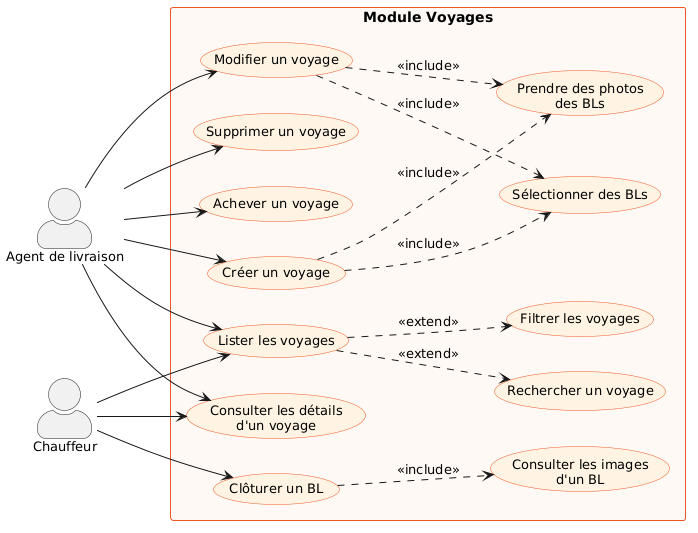
\includegraphics[width=0.85\textwidth]{assets/voyages-use-case.png}
    \caption{Diagramme de cas d'utilisation — Module Voyages}
    \label{fig:voyages-use-case}
    \end{figure}

    Les deux actions détaillées dans la suite illustrent le flux essentiel du module, depuis l'enregistrement d'un départ jusqu'à la preuve de livraison.

    \subsubsection{Créer un voyage}
    Le processus de création d'un voyage est initié par l'agent de livraison. L'utilisateur saisit les informations du voyage — dépôt de départ, chauffeur, véhicule et destination — puis sélectionne les BLs qui seront transportés. Chaque BL sélectionné est photographié afin de conserver une trace visuelle de l'état des documents au moment du chargement. Ces deux étapes — sélection des BLs et prise de photos — sont obligatoires et font partie intégrante du processus de création. Une fois les informations renseignées et les BLs associés au voyage, la création est validée et le voyage est enregistré.

    \begin{figure}[H]
    \centering
    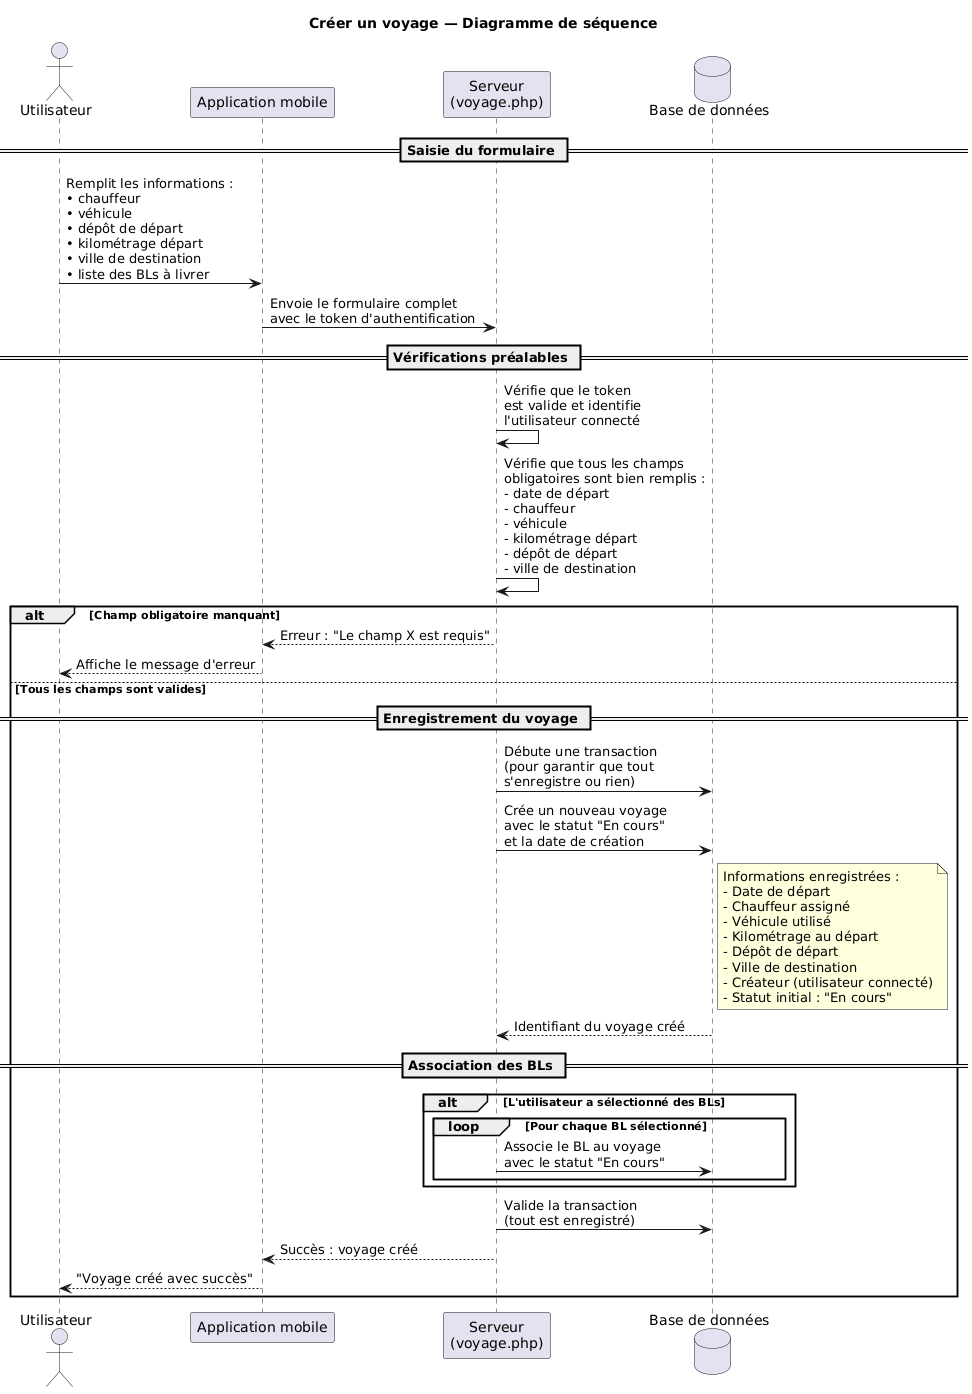
\includegraphics[width=0.85\textwidth]{assets/voyages-create-voyage.png}
    \caption{Cas d'utilisation — Créer un voyage}
    \label{fig:voyages-create-voyage}
    \end{figure}

    \subsubsection{Clôturer un BL}
    La clôture d'un BL est accessible au chauffeur. Cette action intervient lorsque le chauffeur arrive à destination et livre les marchandises. Avant de clôturer le BL, l'utilisateur consulte les images du BL pour vérifier les informations et s'assurer de la conformité de la livraison. La clôture est ensuite confirmée, ce qui marque le BL comme livré.

    \begin{figure}[H]
    \centering
    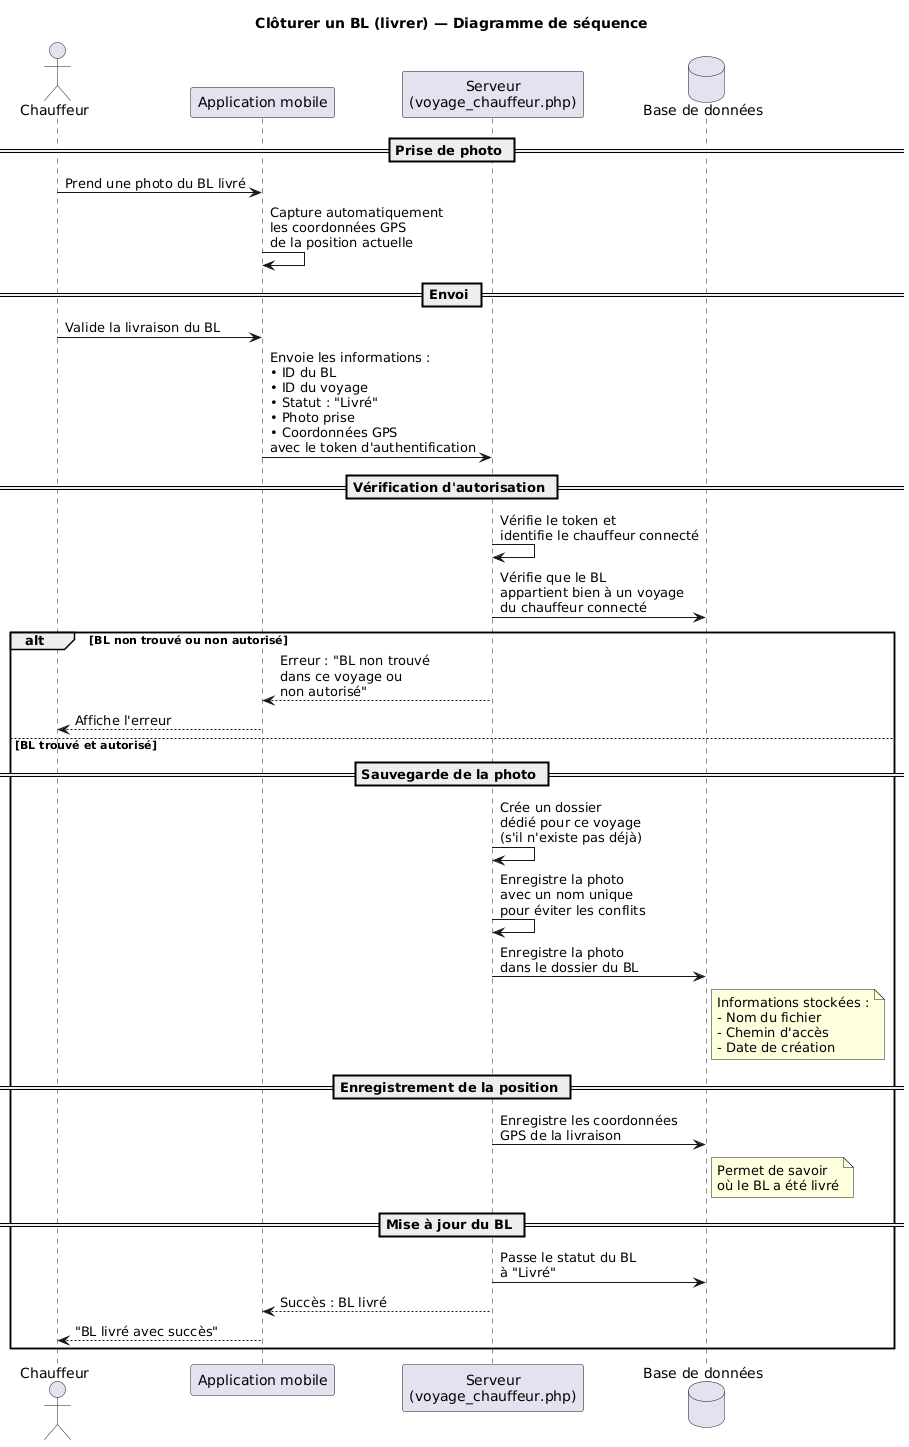
\includegraphics[width=0.85\textwidth]{assets/voyages-cloturer-bl.png}
    \caption{Cas d'utilisation — Clôturer un BL}
    \label{fig:voyages-cloturer-bl}
    \end{figure}

    \subsection{Module Retours}
    Le module Retours fait intervenir deux acteurs : le chauffeur, qui crée, modifie et supprime les retours, et l'agent de caisse, chargé de valider ou refuser les retours. La consultation de la liste est accessible aux deux profils.

    Le diagramme de la Figure~\ref{fig:retours-use-case} présente l'ensemble des cas d'utilisation du module ainsi que les interactions entre ces acteurs.

    \begin{figure}[H]
    \centering
    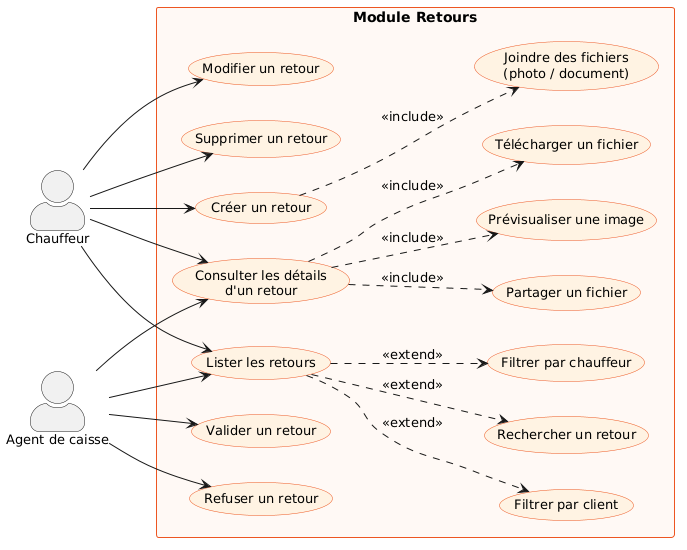
\includegraphics[width=0.85\textwidth]{assets/retours-use-case.png}
    \caption{Diagramme de cas d'utilisation — Module Retours}
    \label{fig:retours-use-case}
    \end{figure}

    Les deux actions détaillées dans la suite illustrent le cycle de vie d'un retour, de sa création par le chauffeur à sa validation par l'agent de caisse.

    \subsubsection{Créer un retour}
    Le processus de création d'un retour est initié par le chauffeur. Ce dernier renseigne les informations du retour — client, dépôt, motif du retour — et joint des documents justificatifs tels que des photos des marchandises retournées. Ces pièces jointes sont obligatoires et font partie intégrante du processus de création. Une fois les informations saisies et les fichiers joints, la création est validée et le retour est enregistré avec le statut \og{}En attente de validation\fg{}.

    \begin{figure}[H]
    \centering
    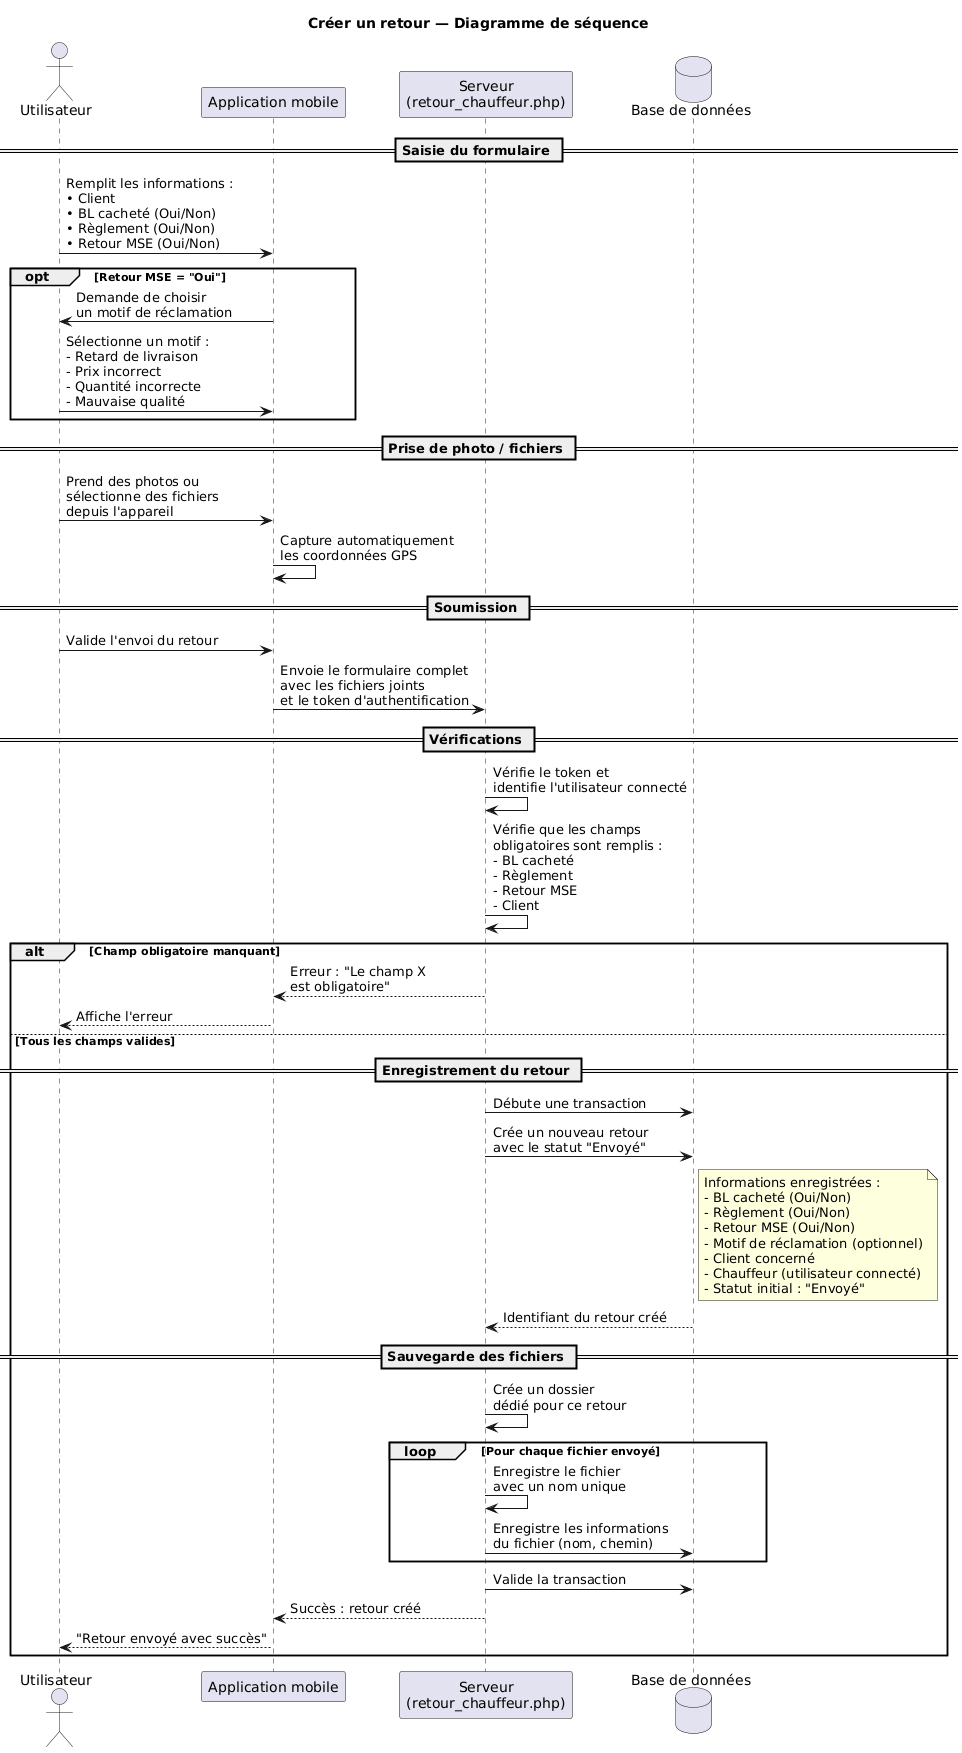
\includegraphics[width=0.85\textwidth]{assets/creer-retour.png}
    \caption{Cas d'utilisation — Créer un retour}
    \label{fig:creer-retour}
    \end{figure}

    \subsubsection{Valider un retour}
    La validation d'un retour est effectuée par l'agent de caisse. Après avoir consulté les détails du retour et examiné les pièces jointes fournies par le chauffeur, l'agent de caisse décide d'accepter ou de refuser le retour. En cas d'acceptation, le statut du retour passe à \og{}Terminé\fg{} ; en cas de refus, il passe à \og{}Refusé\fg{}. Cette étape constitue le point de contrôle final du processus de retour.

    \begin{figure}[H]
    \centering
    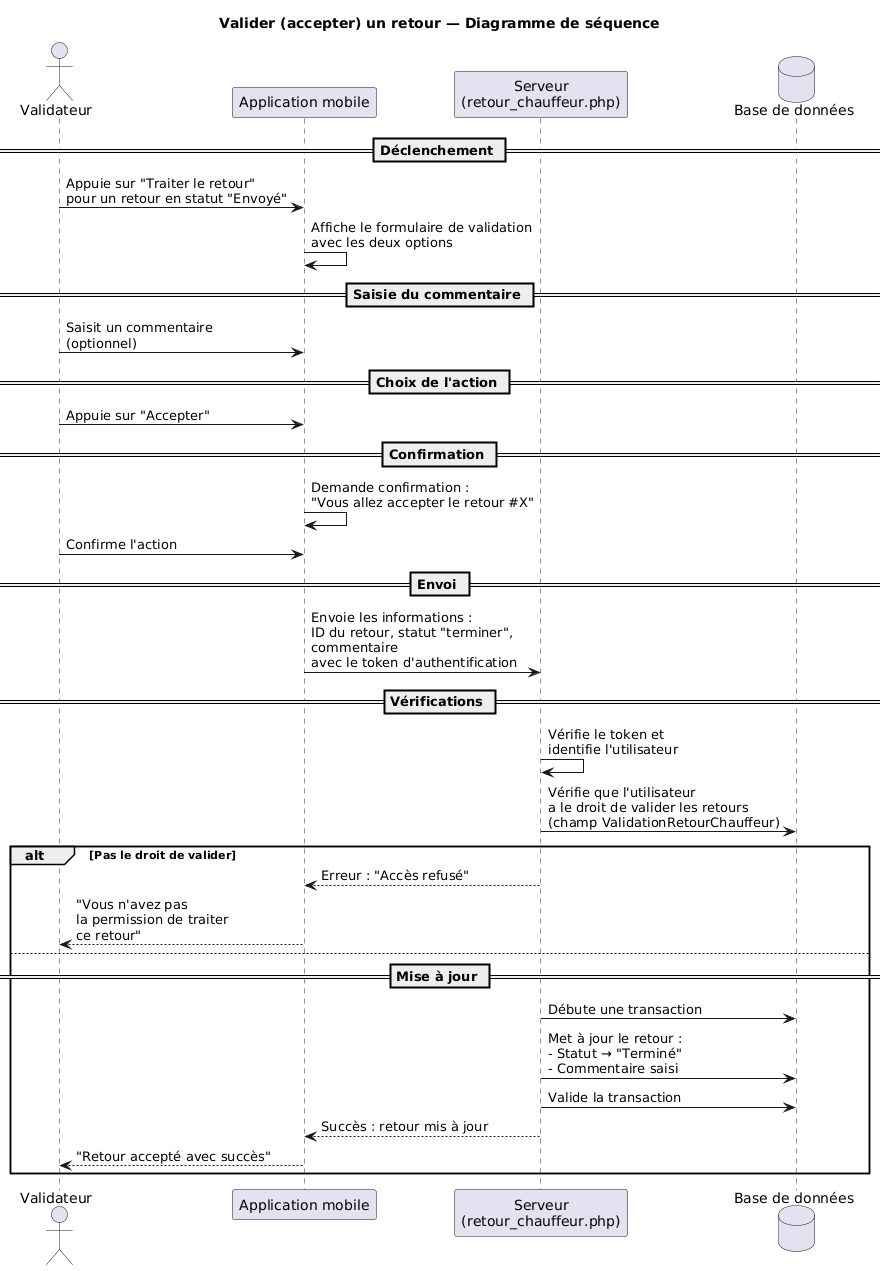
\includegraphics[width=0.85\textwidth]{assets/valider-retour.png}
    \caption{Cas d'utilisation — Valider un retour}
    \label{fig:valider-retour}
    \end{figure}

    \subsection{Module Rapports qualité}
    Le module Rapports qualité fait intervenir deux acteurs : le service import, chargé de créer les rapports qualité, et le contrôle de gestion, qui consulte les rapports. La consultation et le listage sont accessibles aux deux profils.

    Le diagramme de la Figure~\ref{fig:rapports-qualite-use-case} présente l'ensemble des cas d'utilisation du module ainsi que les interactions entre ces acteurs.

    \begin{figure}[H]
    \centering
    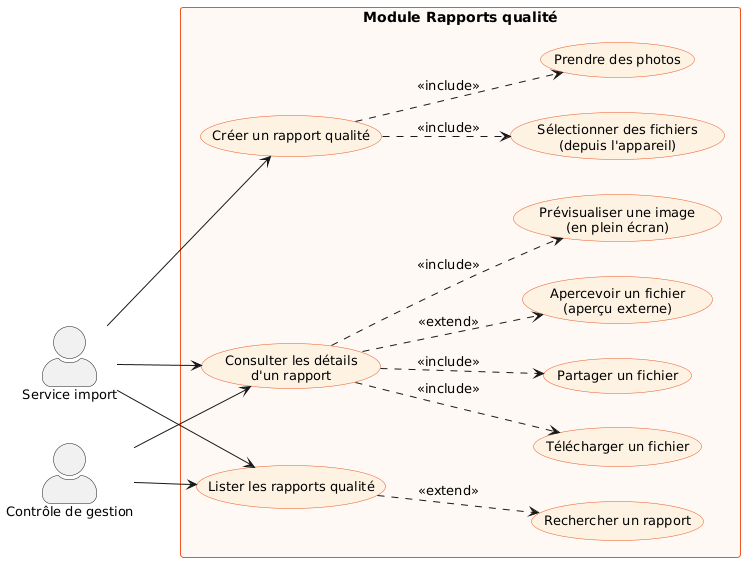
\includegraphics[width=0.85\textwidth]{assets/rapports-qualite-use-case.png}
    \caption{Diagramme de cas d'utilisation — Module Rapports qualité}
    \label{fig:rapports-qualite-use-case}
    \end{figure}

    Les deux actions détaillées dans la suite illustrent le flux du module, depuis la création d'un rapport par le service import jusqu'à sa consultation par le contrôle de gestion.

    \subsubsection{Créer un rapport qualité}
    Le processus de création d'un rapport qualité est initié par le service import. L'utilisateur renseigne les informations du rapport — référence, observations, conformité — et y joint des photos des marchandises ou des documents scannés. Ces pièces jointes permettent de documenter visuellement l'état des produits et constituent un élément essentiel du rapport. Une fois les informations saisies, la création est validée et le rapport est enregistré.

    \begin{figure}[H]
    \centering
    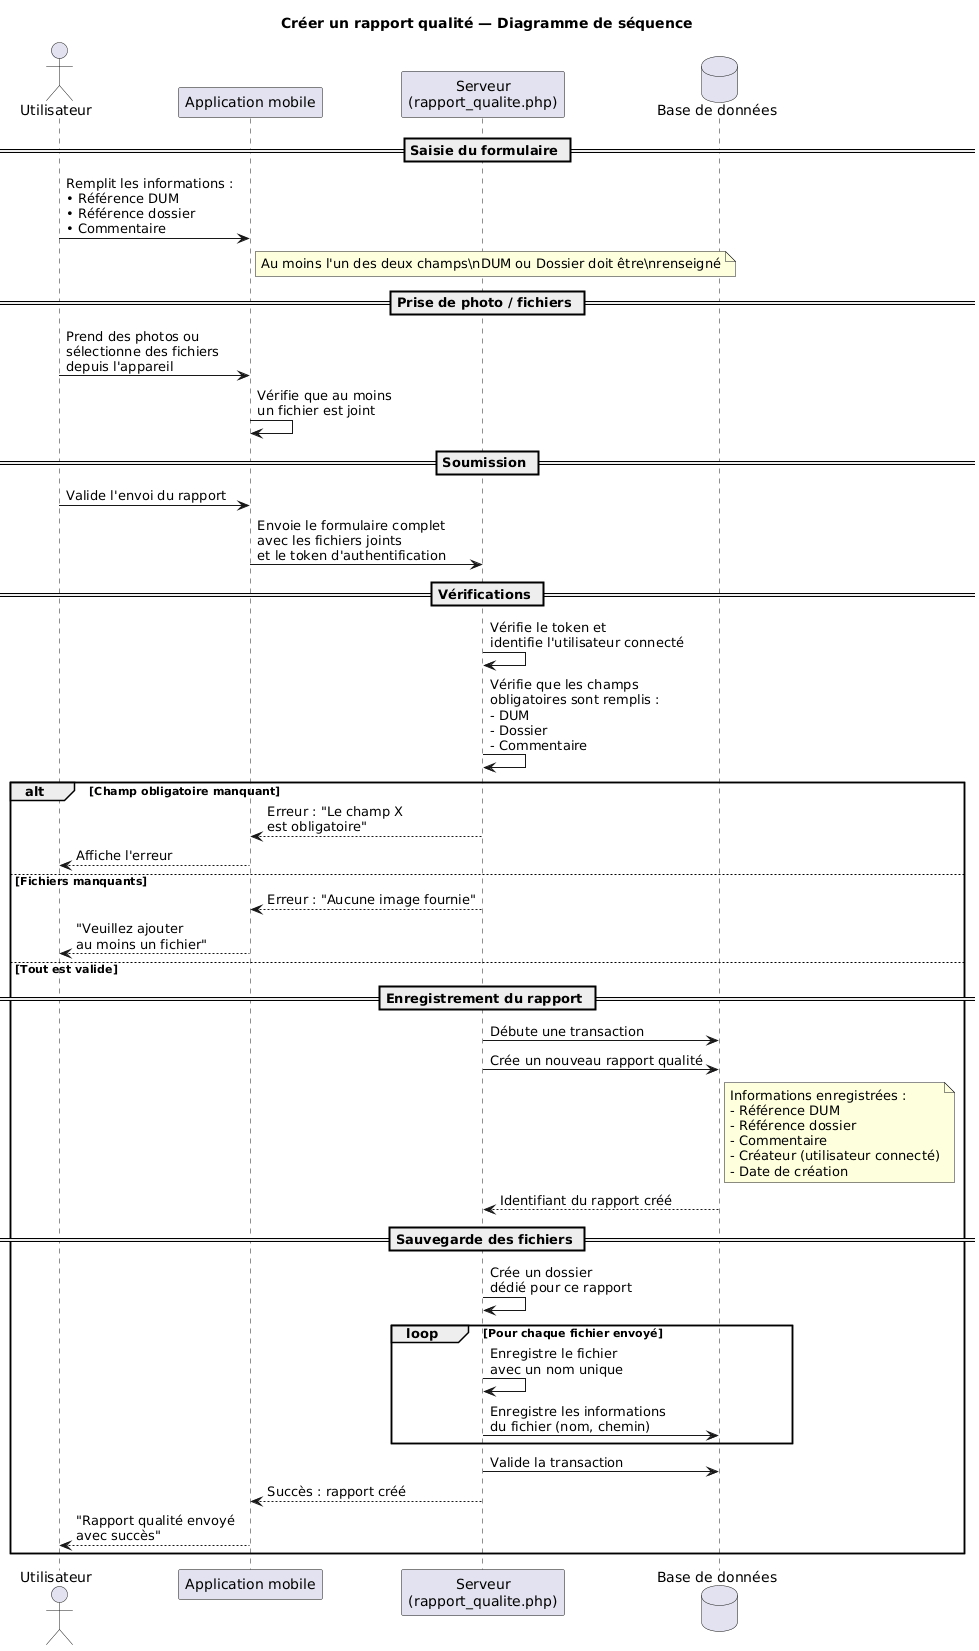
\includegraphics[width=0.85\textwidth]{assets/creer-rapport-qualite.png}
    \caption{Cas d'utilisation — Créer un rapport qualité}
    \label{fig:creer-rapport-qualite}
    \end{figure}

    \subsubsection{Lister les rapports qualité}
    La consultation de la liste des rapports qualité est accessible au service import et au contrôle de gestion. L'utilisateur peut parcourir l'ensemble des rapports enregistrés et utiliser la recherche textuelle pour retrouver un rapport spécifique. Cette fonction permet au contrôle de gestion de suivre l'état qualitatif des marchandises réceptionnées sans intervenir dans le processus de création.

    \begin{figure}[H]
    \centering
    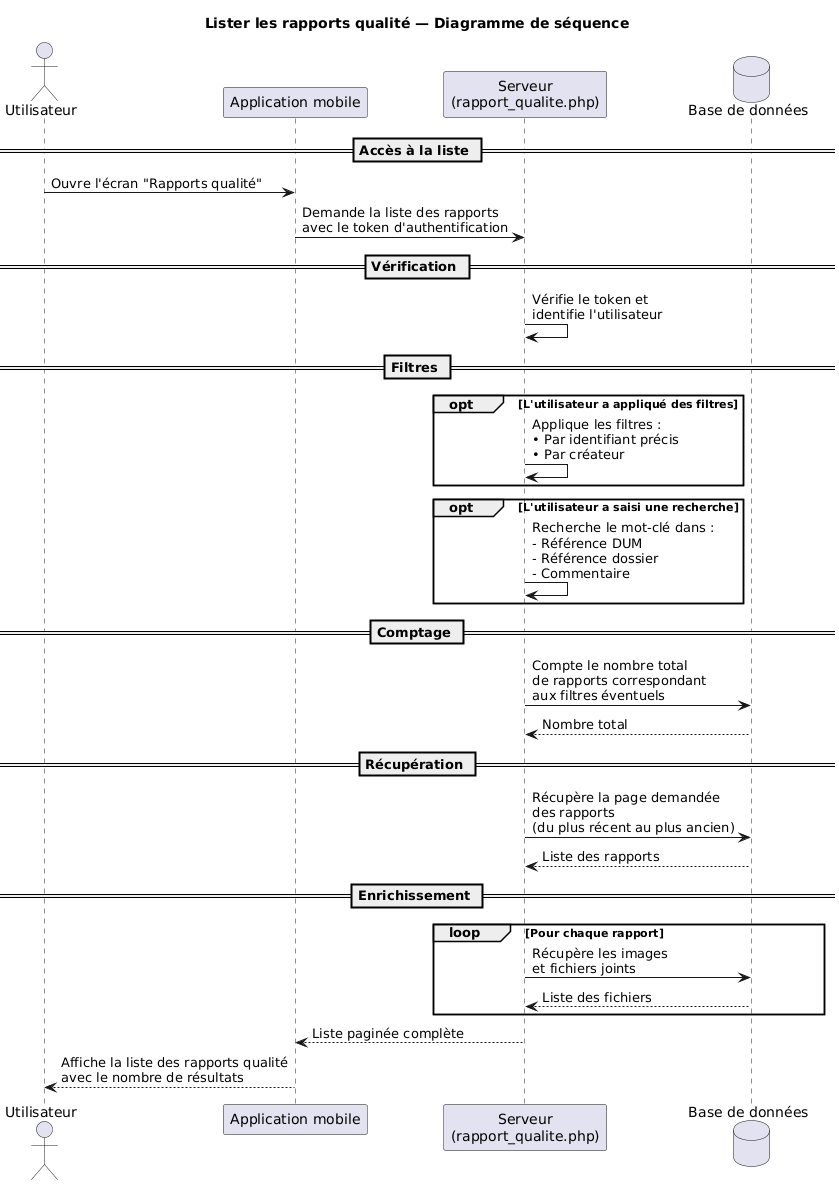
\includegraphics[width=0.85\textwidth]{assets/lister-rapports-qualite.png}
    \caption{Cas d'utilisation — Lister les rapports qualité}
    \label{fig:lister-rapports-qualite}
    \end{figure}

    \subsection{Module Rotation chauffeur}
    Le module Rotation chauffeur fait intervenir un acteur unique : le responsable de flotte. Ce dernier consulte la liste des rotations pour connaître la disponibilité des chauffeurs et des véhicules.

    Le diagramme de la Figure~\ref{fig:rotation-chauffeur-use-case} présente l'ensemble des cas d'utilisation du module.

    \begin{figure}[H]
    \centering
    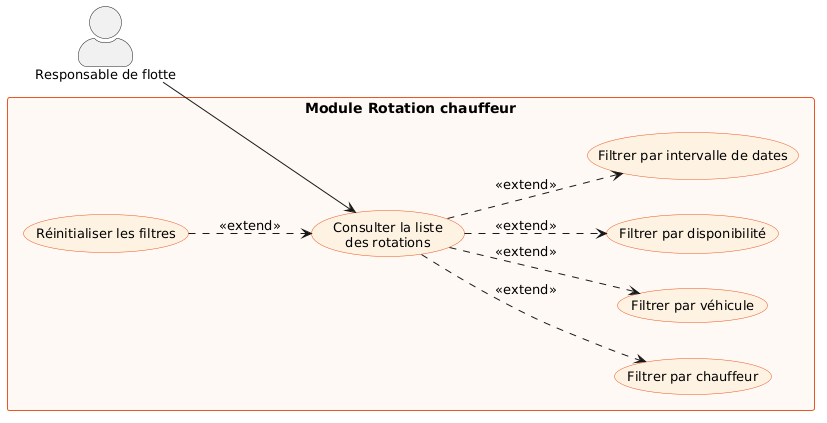
\includegraphics[width=0.85\textwidth]{assets/rotation-chauffeur-use-case.png}
    \caption{Diagramme de cas d'utilisation — Module Rotation chauffeur}
    \label{fig:rotation-chauffeur-use-case}
    \end{figure}

    Une seule action est détaillée pour ce module, la consultation des rotations étant sa fonction principale.

    \subsubsection{Lister les rotations}
    La consultation de la liste des rotations est accessible au responsable de flotte. L'utilisateur peut parcourir l'ensemble des rotations enregistrées et filtrer les résultats par chauffeur, véhicule, disponibilité ou intervalle de dates. Ces filtres permettent d'identifier rapidement quels chauffeurs et véhicules sont disponibles pour une période donnée.

    \begin{figure}[H]
    \centering
    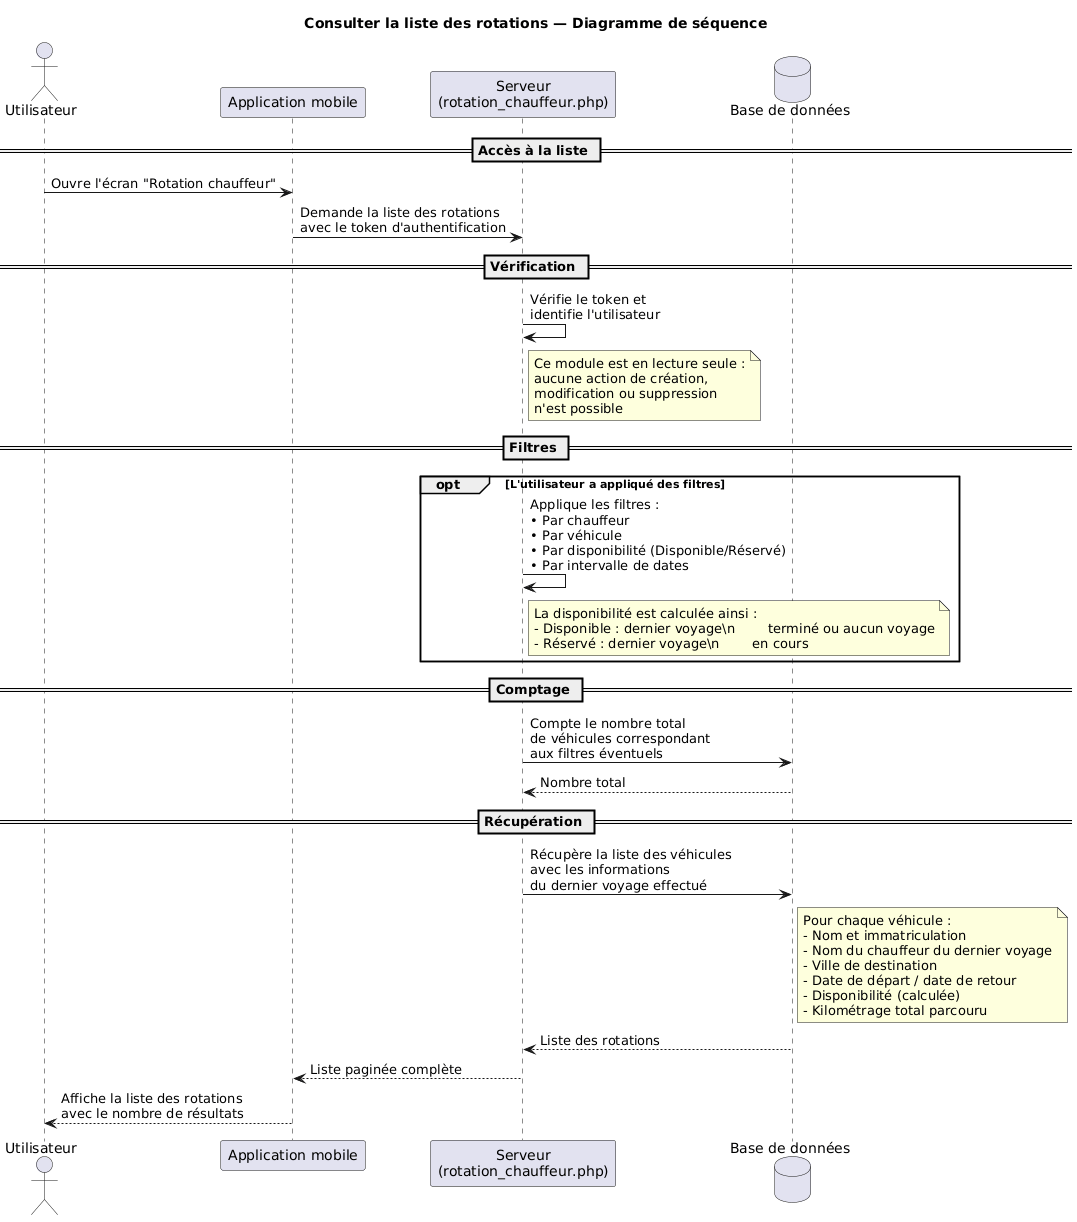
\includegraphics[width=0.85\textwidth]{assets/lister-rotations.png}
    \caption{Cas d'utilisation — Lister les rotations}
    \label{fig:lister-rotations}
    \end{figure}

    \subsection{Module Lieux de projets}
    Le module Lieux de projets fait intervenir plusieurs profils. La création d'un lieu est ouverte à tous les utilisateurs. La consultation et le listage sont réservés au directeur général, au directeur commercial et au directeur adjoint. La modification et la suppression sont réservées au créateur du lieu et au responsable de flotte.

    Le diagramme de la Figure~\ref{fig:lieux-projets-use-case} présente l'ensemble des cas d'utilisation du module ainsi que les interactions entre ces acteurs.

    \begin{figure}[H]
    \centering
    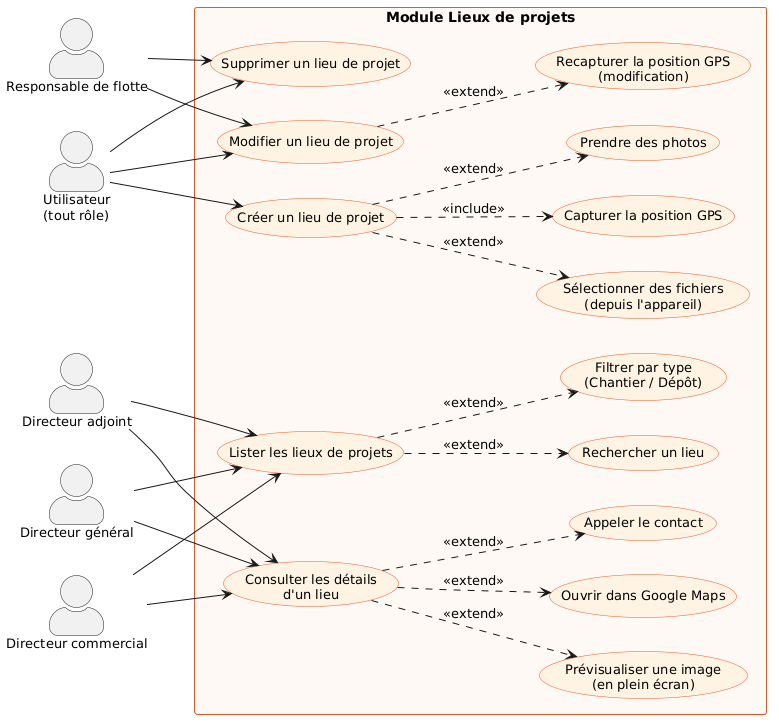
\includegraphics[width=0.85\textwidth]{assets/lieux-projets-use-case.png}
    \caption{Diagramme de cas d'utilisation — Module Lieux de projets}
    \label{fig:lieux-projets-use-case}
    \end{figure}

    Les deux actions détaillées dans la suite illustrent le flux du module, de la création d'un lieu par un utilisateur à sa consultation par les directeurs.

    \subsubsection{Créer un lieu de projet}
    Le processus de création d'un lieu de projet est accessible à tous les utilisateurs. Ces derniers renseignent le nom, le type (chantier ou dépôt), l'adresse, le contact et capturent automatiquement les coordonnées GPS. Des photos du lieu peuvent être jointes afin de documenter visuellement le projet. Une fois les informations saisies, la création est validée et le lieu est enregistré.

    \begin{figure}[H]
    \centering
    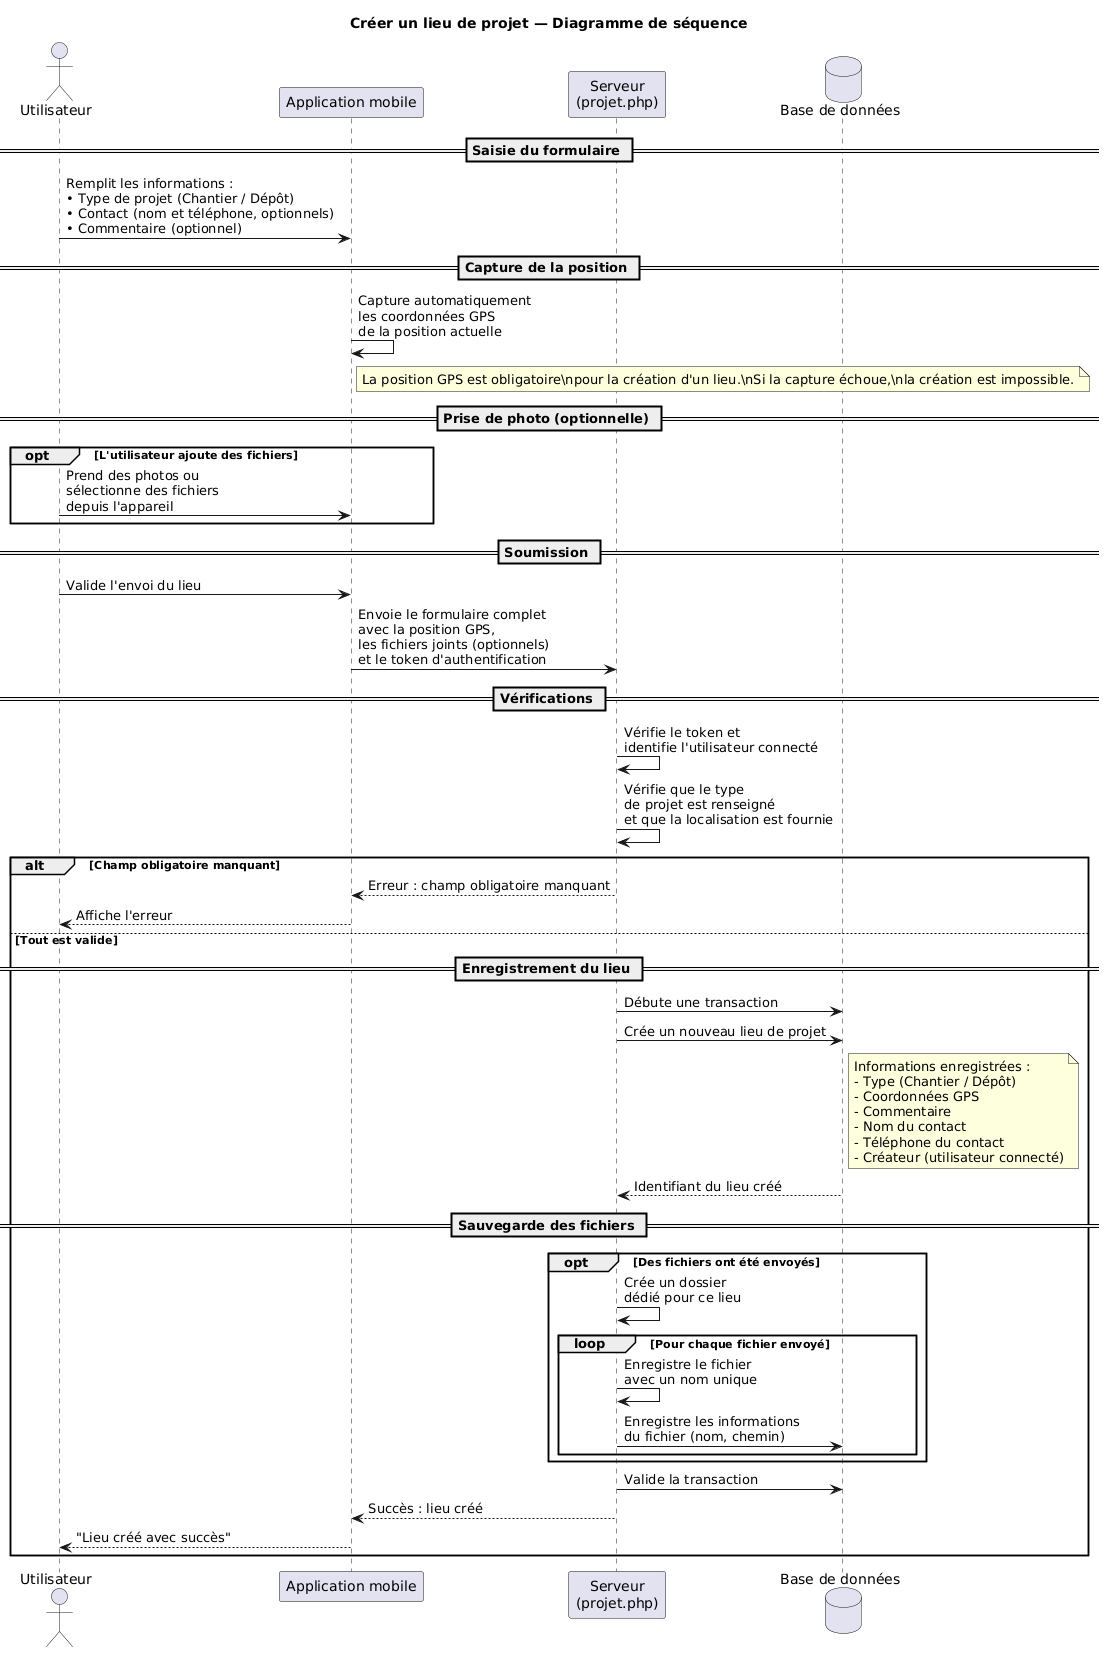
\includegraphics[width=0.85\textwidth]{assets/creer-lieu-projet.png}
    \caption{Cas d'utilisation — Créer un lieu de projet}
    \label{fig:creer-lieu-projet}
    \end{figure}

    \subsubsection{Lister les lieux de projets}
    La consultation de la liste des lieux de projets est accessible au directeur général, au directeur commercial et au directeur adjoint. L'utilisateur peut parcourir l'ensemble des lieux enregistrés, filtrer par type (chantier ou dépôt) et utiliser la recherche textuelle pour retrouver un lieu spécifique.

    \begin{figure}[H]
    \centering
    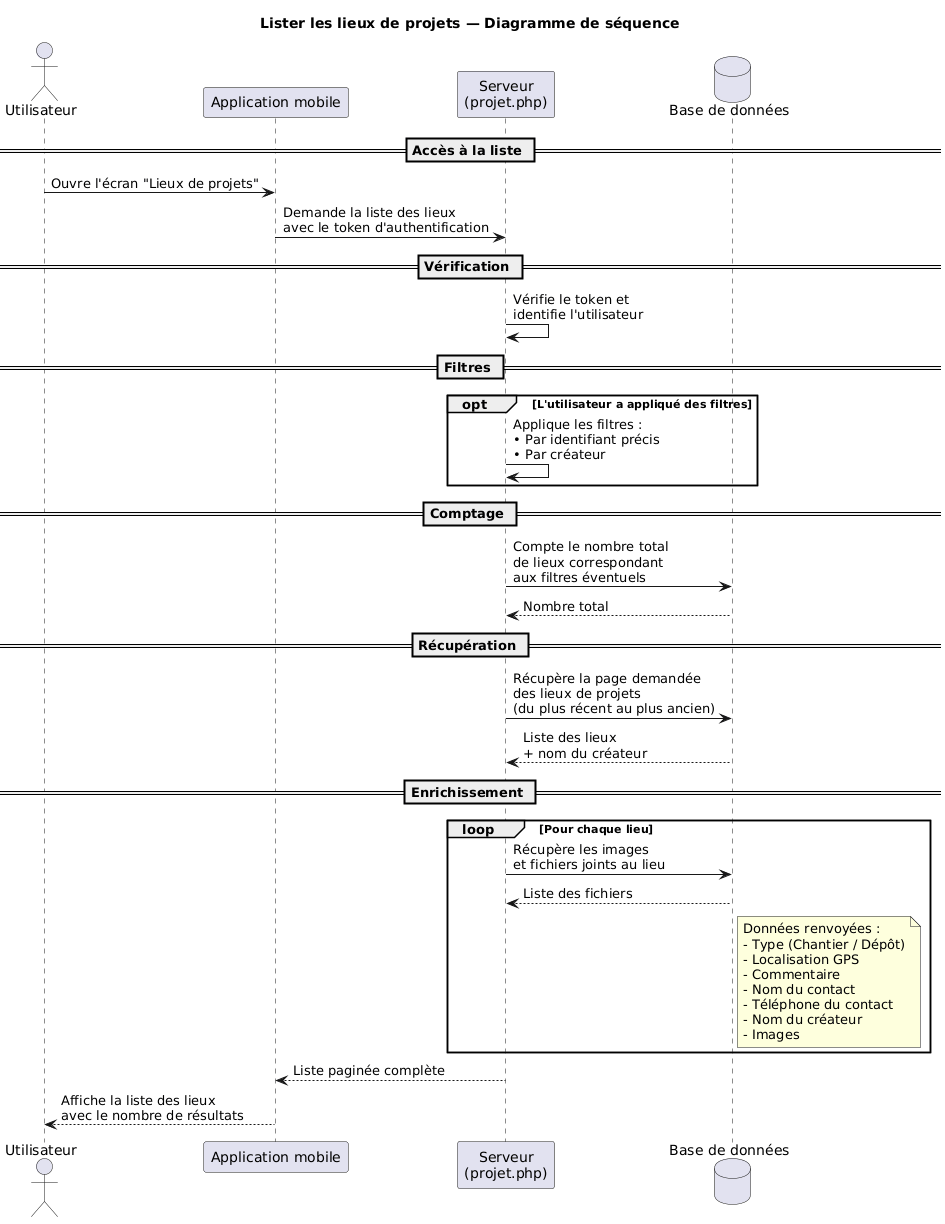
\includegraphics[width=0.85\textwidth]{assets/lister-lieux-projets.png}
    \caption{Cas d'utilisation — Lister les lieux de projets}
    \label{fig:lister-lieux-projets}
    \end{figure}

    \subsection{Module Demande de transfert}
    Le module Demande de transfert fait intervenir trois acteurs : l'ADV (agent des ventes) et le responsable de stock, qui créent les demandes, ajoutent et suppriment les produits et gèrent leurs lots, et le magasinier, chargé de la préparation des produits et des lots. La consultation de la liste est accessible aux créateurs de demandes et aux magasiniers.

    Le diagramme de la Figure~\ref{fig:demande-transfert-use-case} présente l'ensemble des cas d'utilisation du module ainsi que les interactions entre ces acteurs.

    \begin{figure}[H]
    \centering
    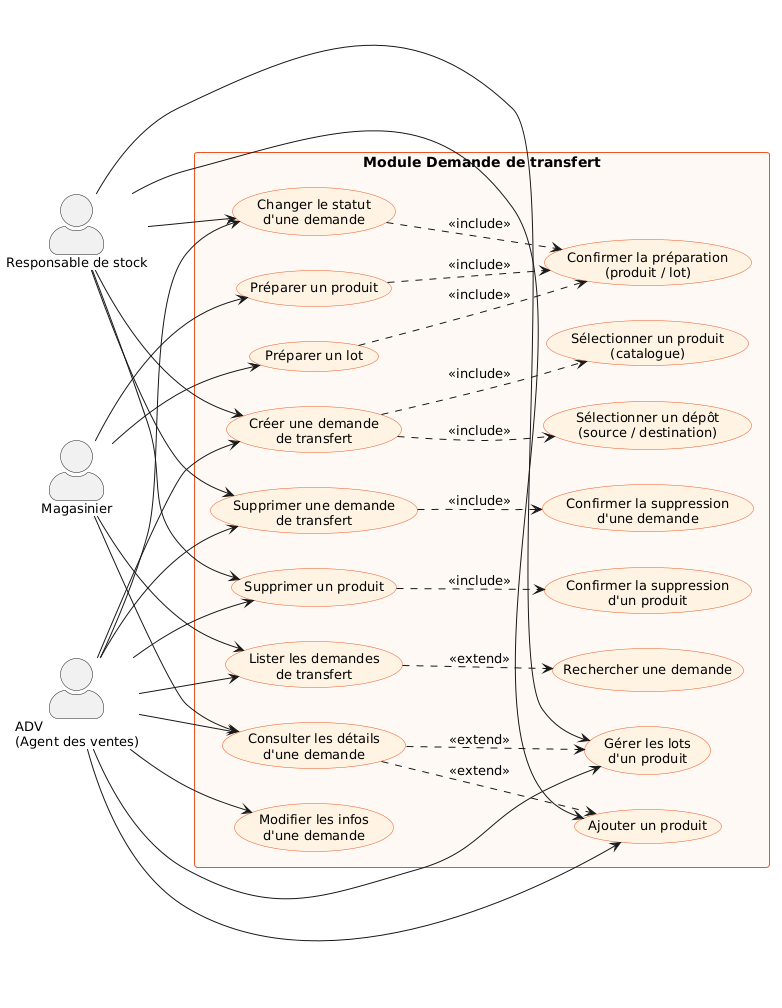
\includegraphics[width=0.85\textwidth]{assets/demande-transfert-use-case.png}
    \caption{Diagramme de cas d'utilisation — Module Demande de transfert}
    \label{fig:demande-transfert-use-case}
    \end{figure}

    Les trois actions détaillées dans la suite illustrent le flux du module, de la création d'une demande jusqu'à la préparation des produits par le magasinier.

    \subsubsection{Créer une demande de transfert}
    Le processus de création d'une demande de transfert est initié par l'ADV ou le responsable de stock. L'utilisateur sélectionne un dépôt source et un dépôt de destination, puis ajoute les produits concernés depuis le catalogue. Pour chaque produit, il renseigne la quantité souhaitée puis sélectionne les lots à transférer. Une fois tous les produits ajoutés, la création est validée et la demande est enregistrée avec le statut \og{}Brouillon\fg{}.

    \begin{figure}[H]
    \centering
    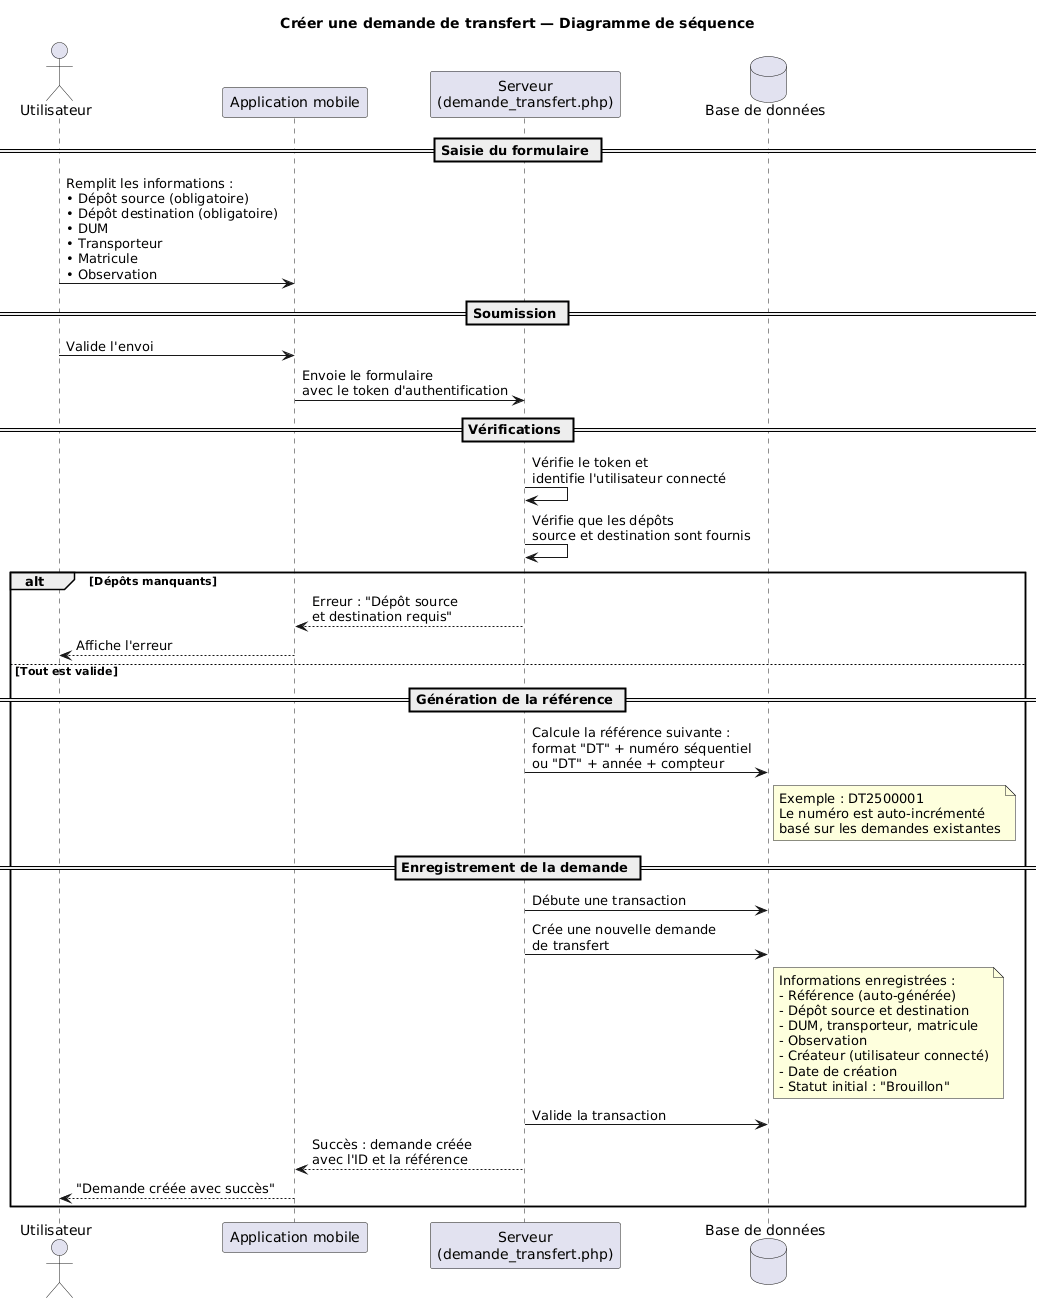
\includegraphics[width=0.85\textwidth]{assets/creer-demande-transfert.png}
    \caption{Cas d'utilisation — Créer une demande de transfert}
    \label{fig:creer-demande-transfert}
    \end{figure}

    \subsubsection{Gérer les lots d'un produit}
    La gestion des lots d'un produit est effectuée par l'ADV ou le responsable de stock après l'ajout d'un produit à la demande. L'utilisateur accède à la liste des lots disponibles pour le produit sélectionné et choisit les lots à inclure dans le transfert. Il peut ajouter de nouveaux lots ou retirer des lots déjà sélectionnés, à l'exception des lots déjà préparés qui ne peuvent plus être modifiés.

    \begin{figure}[H]
    \centering
    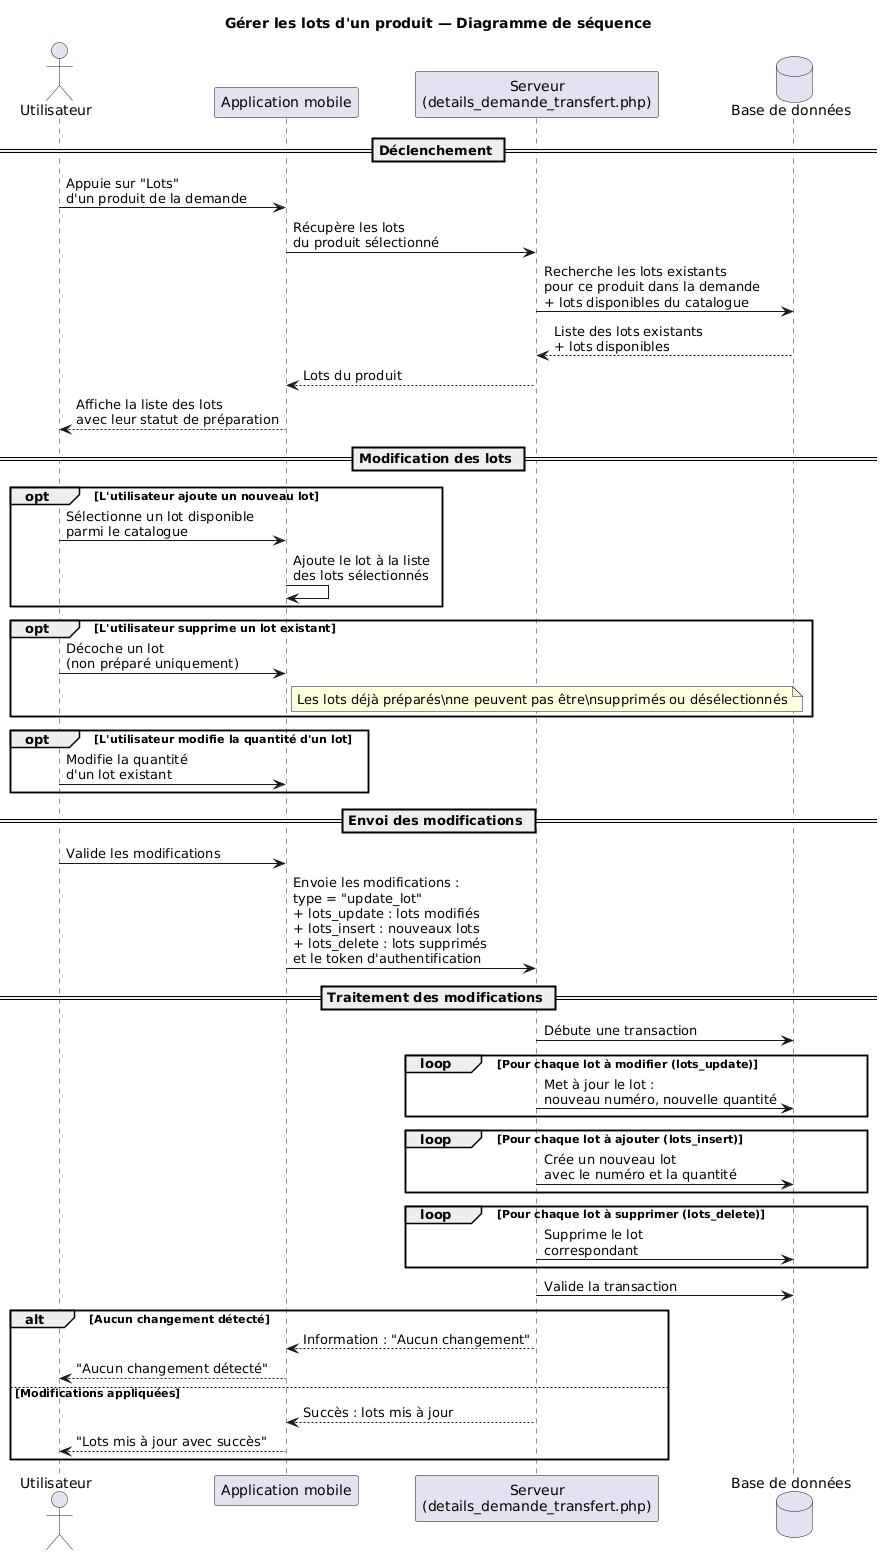
\includegraphics[width=0.85\textwidth]{assets/gerer-lots-demande-transfert.png}
    \caption{Cas d'utilisation — Gérer les lots d'un produit}
    \label{fig:gerer-lots-demande-transfert}
    \end{figure}

    \subsubsection{Préparer un produit ou un lot}
    La préparation des produits et des lots est la tâche exclusive du magasinier. Ce dernier consulte la liste des demandes de transfert et, pour chaque demande, prépare physiquement les produits demandés. Il peut marquer un produit entier comme préparé ou préparer des lots individuellement. Une fois un produit ou un lot marqué comme préparé, il ne peut plus être modifié ou retiré de la demande.

    \begin{figure}[H]
    \centering
    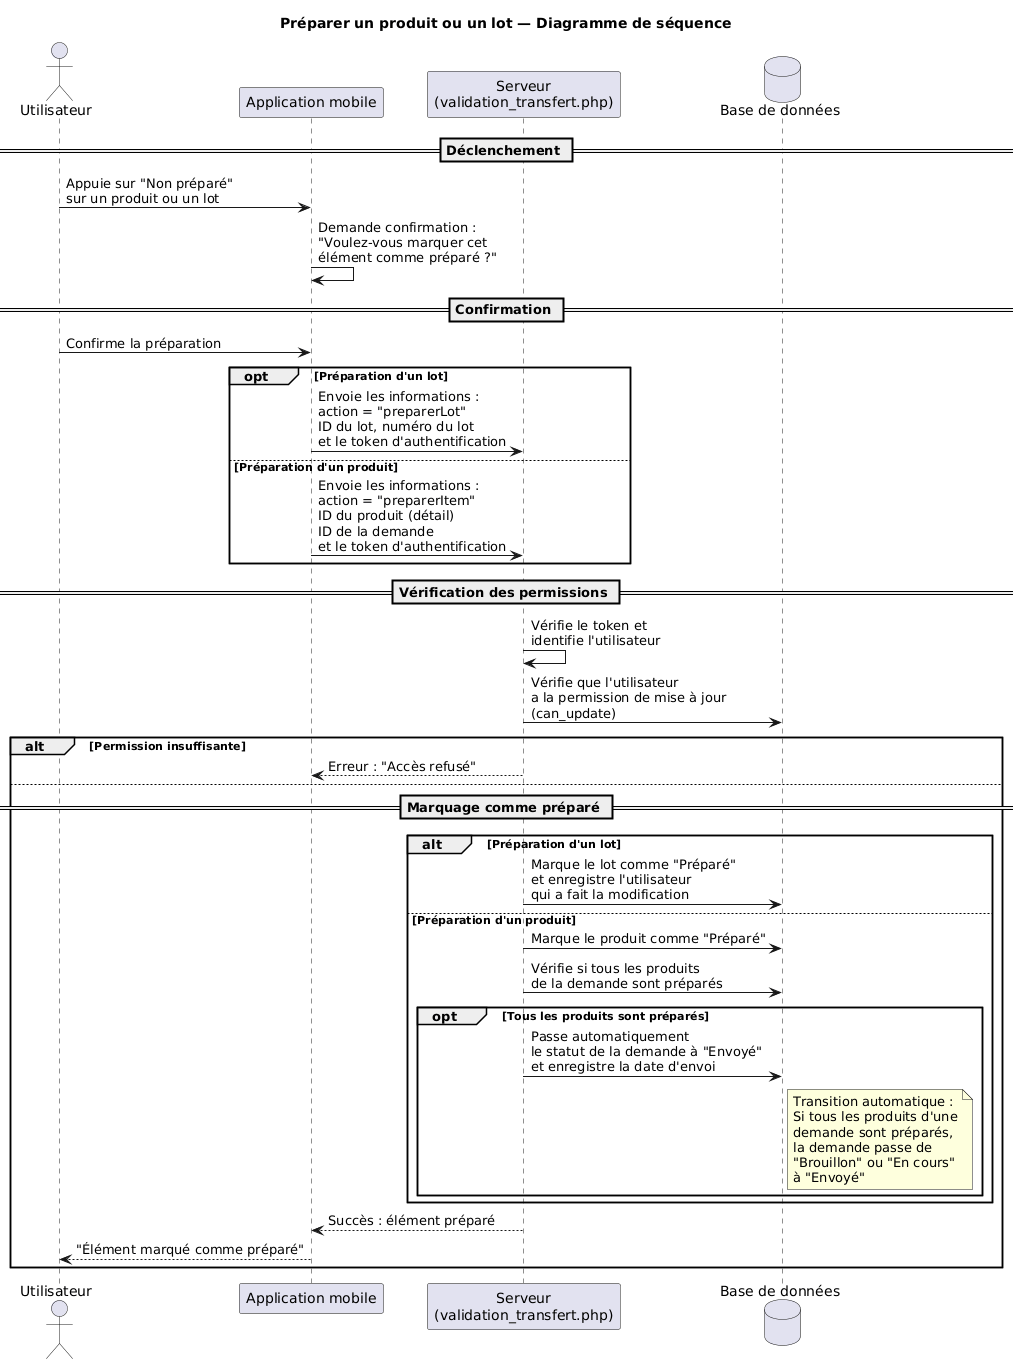
\includegraphics[width=0.85\textwidth]{assets/preparer-produit-lot-demande-transfert.png}
    \caption{Cas d'utilisation — Préparer un produit ou un lot}
    \label{fig:preparer-produit-lot-demande-transfert}
    \end{figure}

\subsection{Conclusion du chapitre}
Ce chapitre a présenté l'analyse des besoins et la modélisation de la solution. L'analyse fonctionnelle a permis d'identifier les besoins de chaque module métier — voyages, retours chauffeur, rapports qualité, rotation chauffeur, lieux de projets et demandes de transfert — ainsi que les besoins non fonctionnels en matière de performance, sécurité, ergonomie, maintenabilité et disponibilité. La modélisation UML a ensuite traduit ces besoins en cas d'utilisation concrets, en identifiant les acteurs impliqués et leurs interactions avec le système.

La répartition des responsabilités entre les différents rôles métier a été mise en évidence : agent de livraison et chauffeur pour les voyages, chauffeur et agent de caisse pour les retours, service import et contrôle de gestion pour les rapports qualité, responsable de flotte pour la rotation, ADV/responsable de stock et magasinier pour les demandes de transfert, et l'ensemble des profils pour les lieux de projets. Le rôle admin global, attribué au Directeur Général et au Directeur Général Adjoint, garantit un accès transversal à toutes les fonctionnalités de l'application.

Les actions détaillées pour chaque module illustrent les flux essentiels : de la création à la validation, de la préparation à la livraison. Ces spécifications et cette modélisation constituent le socle à partir duquel l'architecture technique et l'implémentation ont été réalisées.

    \newpage
    \thispagestyle{empty}
    \vspace*{\fill}
    \begin{center}
    {\Huge \textbf{CHAPITRE 3}}\\[0.8em]
    {\LARGE \textbf{MISE EN ŒUVRE DE LA\\[0.4em]SOLUTION}}
    \end{center}
    \vspace*{\fill}

    \newpage
    \renewcommand{\thesection}{3.\arabic{section}}
    \setcounter{section}{0}

\addcontentsline{toc}{section}{{\bfseries Chapitre 3 : Mise en œuvre de la solution}}

    \section{Introduction}
    Ce troisième chapitre présente les différentes technologies et outils adoptés pour le développement de la solution proposée. En outre, il représente la modélisation du processus final et détaille les différentes étapes de la réalisation de ce projet, en se servant de captures illustratives.

    \section{Outils utilisés}

    \subsection{Environnements de développement}

    \begin{minipage}[t]{0.16\textwidth}
    \centering
    \IfFileExists{assets/vscode-logo.png}{
\includegraphics[width=\linewidth]{assets/vscode-logo.png}}{\textit{VS Code}}
    \end{minipage}\hfill
    \begin{minipage}[t]{0.80\textwidth}
    \textbf{Visual Studio Code (VS Code)} : éditeur de code libre et multiplateforme développé par Microsoft. Léger, extensible et doté d'un écosystème riche d'extensions, il a été utilisé pour l'édition du code frontend et backend, le débogage et la gestion de terminal intégré. \textit{Justification :} VS Code a été choisi pour sa légèreté, son support natif de TypeScript et PHP, et ses extensions intégrées pour Git, React Native et le débogage mobile.
    \end{minipage}\\[0.8em]

    \begin{minipage}[t]{0.16\textwidth}
    \centering
    \IfFileExists{assets/git-logo.png}{
\includegraphics[width=\linewidth]{assets/git-logo.png}}{\textit{Git}}
    \end{minipage}\hfill
    \begin{minipage}[t]{0.80\textwidth}
    \textbf{Git} : système de gestion de versions distribué qui permet de suivre chaque modification du code source, de créer des branches de développement et de fusionner les contributions. Il garantit la traçabilité des évolutions et facilite le travail collaboratif. \textit{Justification :} Git est le standard industriel pour le contrôle de version ; il permet de revenir à tout état antérieur du code, de travailler en parallèle sur plusieurs fonctionnalités et de conserver un historique complet des modifications.
    \end{minipage}\\[0.8em]

    \begin{minipage}[t]{0.16\textwidth}
    \centering
    \IfFileExists{assets/github-logo.png}{
\includegraphics[width=\linewidth]{assets/github-logo.png}}{\textit{GitHub}}
    \end{minipage}\hfill
    \begin{minipage}[t]{0.80\textwidth}
    \textbf{GitHub} : plateforme d'hébergement de dépôts Git qui offre un espace centralisé pour le stockage du code, la revue de contributions via les pull requests et le suivi des tickets. Elle sécurise le code distant et permet un accès partagé à l'équipe. \textit{Justification :} GitHub fournit un dépôt distant fiable, accessible de n'importe où, et facilite le suivi des problèmes et la collaboration entre développeurs via les pull requests.
    \end{minipage}\\[0.8em]

    \begin{minipage}[t]{0.16\textwidth}
    \centering
    \IfFileExists{assets/postman-logo.png}{
\includegraphics[width=\linewidth]{assets/postman-logo.png}}{\textit{Postman}}
    \end{minipage}\hfill
    \begin{minipage}[t]{0.80\textwidth}
    \textbf{Postman} : outil de test et de documentation d'API REST. Il permet de construire, envoyer et inspecter des requêtes HTTP vers les endpoints du backend, de vérifier les réponses et d'organiser les tests en collections réutilisables. \textit{Justification :} Postman a été indispensable pour valider chaque endpoint de l'API PHP au fur et à mesure du développement, vérifier les réponses et les codes d'erreur, et documenter les requêtes pour le frontend.
    \end{minipage}\\[0.8em]

    \begin{minipage}[t]{0.16\textwidth}
    \centering
    \IfFileExists{assets/phpmyadmin-logo.png}{
\includegraphics[width=\linewidth]{assets/phpmyadmin-logo.png}}{\textit{phpMyAdmin}}
    \end{minipage}\hfill
    \begin{minipage}[t]{0.80\textwidth}
    \textbf{phpMyAdmin} : interface web d'administration de bases de données MySQL. Elle permet de gérer les bases, les tables, les utilisateurs et les permissions, d'exécuter des requêtes SQL et d'importer ou exporter des données, le tout sans recourir à la ligne de commande. \textit{Justification :} phpMyAdmin offre un accès visuel rapide à la base de données pour créer les tables, vérifier les données et déboguer les requêtes, sans installer d'outil supplémentaire sur le serveur.
    \end{minipage}

    \subsection{Base de données}

    \begin{minipage}[t]{0.16\textwidth}
    \centering
    \IfFileExists{assets/mysql-logo.png}{
\includegraphics[width=\linewidth]{assets/mysql-logo.png}}{\textit{MySQL}}
    \end{minipage}\hfill
    \begin{minipage}[t]{0.80\textwidth}
    \textbf{MySQL} : système de gestion de bases de données relationnelles (SGBD) open source, fondé sur le langage SQL (Structured Query Language). SQL permet de définir la structure des données (création de tables, contraintes d'intégrité, clés étrangères), de les manipuler (insertion, mise à jour, suppression) et de les interroger de manière déclarative.
    \end{minipage}

    Le choix de MySQL repose sur plusieurs critères : sa maturité et sa fiabilité éprouvées dans les environnements de production, ses performances élevées en lecture et en écriture pour des volumes de données conséquents, sa conformité aux standards SQL qui garantit la portabilité des requêtes, et son intégration native avec PHP via l'extension MySQLi. L'ensemble des données métier — voyages, retours, rapports qualité, demandes de transfert, lieux de projets, utilisateurs et permissions — est stocké dans une base MySQL hébergée sur le serveur de l'entreprise. \textit{Justification :} MySQL a été choisi pour sa compatibilité directe avec PHP, sa robustesse en production et sa disponibilité sur l'infrastructure existante de SDK WOOD.

    \subsection{Langage de programmation backend}

    \begin{minipage}[t]{0.16\textwidth}
    \centering
    \IfFileExists{assets/php-logo.png}{
\includegraphics[width=\linewidth]{assets/php-logo.png}}{\textit{PHP}}
    \end{minipage}\hfill
    \begin{minipage}[t]{0.80\textwidth}
    \textbf{PHP} : langage de script côté serveur conçu pour le développement web. Dans ce projet, PHP a été utilisé en tant que langage pur, sans recours à un framework. L'objectif de ce choix est double : d'une part, conserver une totale maîtrise de la logique métier et de la structure du code, sans les abstractions et les conventions imposées par un framework ; d'autre part, s'adapter à l'environnement de travail existant au sein de SDK WOOD, où PHP est la technologie backend en place. Ce choix permet ainsi à l'équipe interne de modifier, étendre et maintenir le code source du backend sans courbe d'apprentissage liée à un framework supplémentaire.
    \end{minipage}

    Parmi les avantages de PHP sans framework : une exécution directe sur le serveur web Apache, une configuration minimale, un cycle requête-réponse simple et un déploiement immédiat par simple transfert de fichiers. Chaque endpoint de l'API correspond à un fichier PHP dédié, ce qui favorise la lisibilité, la traçabilité et la maintenabilité. \textit{Justification :} PHP a été adopté pour s'insérer naturellement dans l'environnement technique existant de SDK WOOD, permettant à l'équipe interne de reprendre et faire évoluer le code sans dépendance à un framework.

    \subsection{Langage de programmation frontend}

    \begin{minipage}[t]{0.16\textwidth}
    \centering
    \IfFileExists{assets/typescript-logo.png}{
\includegraphics[width=\linewidth]{assets/typescript-logo.png}}{\textit{TypeScript}}
    \end{minipage}\hfill
    \begin{minipage}[t]{0.80\textwidth}
    \textbf{TypeScript} : sur-ensemble de JavaScript développé par Microsoft, ajoutant un typage statique optionnel au langage. Par rapport à JavaScript, TypeScript détecte les erreurs de type à la compilation plutôt qu'à l'exécution, améliore l'autocomplétion et la navigation dans l'éditeur de code, et facilite la refactorisation grâce à une meilleure analyse statique. Le typage explicite des props, des états et des réponses API réduit les erreurs de régression et documente le contrat entre le frontend et le backend, ce qui est particulièrement précieux dans un projet mobile où les champs et les formats de données sont nombreux. \textit{Justification :} TypeScript a été choisi pour réduire les erreurs à l'exécution grâce au typage statique, améliorer la productivité via l'autocomplétion, et faciliter la maintenance du code dans un projet comptant de nombreux types de données échangés avec l'API.
    \end{minipage}\\[0.8em]

    \begin{minipage}[t]{0.16\textwidth}
    \centering
    \IfFileExists{assets/react-native-logo.png}{
\includegraphics[width=\linewidth]{assets/react-native-logo.png}}{\textit{React Native}}
    \end{minipage}\hfill
    \begin{minipage}[t]{0.80\textwidth}
    \textbf{React Native} : framework développé par Meta permettant de construire des applications mobiles natives pour iOS et Android à partir d'une base de code unique en JavaScript/TypeScript. Contrairement à une approche hybride basée sur un navigateur embarqué, React Native génère de véritables composants natifs : les éléments d'interface déclarés en React sont traduits en vues UIKit sur iOS et en vues Android sur Android, via un pont (Bridge) qui assure la communication entre le thread JavaScript et le thread natif. Ce mécanisme permet de bénéficier des performances et du rendu natifs tout en conservant un cycle de développement rapide — rechargement instantané, métrologie en temps réel et partage de logique métier entre les deux plateformes.
    \end{minipage}

    Par rapport au développement natif en Java (Android) ou Objective-C/Swift (iOS), React Native offre un gain de productivité substantiel : une seule base de code pour deux plateformes, un écosystème de bibliothèques riche via npm, et une communauté active. Le choix de React Native pour ce projet se justifie par la nécessité de livrer une application mobile robuste et performante dans un délai contraint, tout en ciblant simultanément les environnements Android et iOS. \textit{Justification :} React Native a été retenu pour sa capacité à produire une application native pour iOS et Android à partir d'un code unique, réduisant les coûts de développement et les délais tout en offrant des performances proches du natif.

    \begin{minipage}[t]{0.16\textwidth}
    \centering
    \IfFileExists{assets/expo-logo.png}{
\includegraphics[width=\linewidth]{assets/expo-logo.png}}{\textit{Expo}}
    \end{minipage}\hfill
    \begin{minipage}[t]{0.80\textwidth}
    \textbf{Expo} : plateforme de développement et de déploiement construite au-dessus de React Native. Elle fournit un ensemble d'outils et de services — SDK, serveur de développement, builds cloud et application de prévisualisation — qui simplifient le cycle de développement mobile. Expo élimine la nécessité de configurer nativement Android Studio et Xcode : un simple \texttt{expo start} lance un serveur de développement avec rechargement en temps réel, l'application Expo Go permet de tester directement sur un appareil physique sans compilation, et les builds gérés (EAS Build) produisent les APK et IPA prêts pour la distribution. \textit{Justification :} Expo a été adopté pour accélérer le développement en supprimant la configuration native, permettre des itérations rapides via le rechargement instantané sur appareil, et simplifier la génération de l'APK de production sans environnement Android Studio.
    \end{minipage}\\[0.8em]

    \begin{minipage}[t]{0.16\textwidth}
    \centering
    \IfFileExists{assets/android-studio-logo.png}{
\includegraphics[width=\linewidth]{assets/android-studio-logo.png}}{\textit{Android Studio}}
    \end{minipage}\hfill
    \begin{minipage}[t]{0.80\textwidth}
    \textbf{Android Studio} : environnement de développement intégré (IDE) officiel pour le développement Android, développé par Google. Bien que le framework Expo simplifie considérablement la configuration native, Android Studio reste indispensable au projet pour deux raisons : la génération du fichier APK de production via un build de développement (\textit{development build}) et le lancement d'émulateurs Android pour tester l'application sur différentes versions et tailles d'écran sans nécessiter de périphérique physique. \textit{Justification :} Android Studio a été utilisé comme outil complémentaire à Expo pour la compilation native et l'émulation, assurant la compatibilité de l'application avec l'écosystème Android.
    \end{minipage}

    \section{Bibliothèques et packages TypeScript}

    Le frontend de l'application repose sur un ensemble de bibliothèques TypeScript sélectionnées pour couvrir la navigation, la gestion d'état, les appels réseau, les interactions utilisateur et l'accès aux fonctionnalités natives. Le Tableau~\ref{tab:packages-ts} présente les packages principaux et leur usage dans le projet.

    \begin{table}[H]
    \centering
    \renewcommand{\arraystretch}{1.3}
    \caption{Packages TypeScript principaux du frontend}
    \label{tab:packages-ts}
    \begin{tabular}{|p{4.5cm}|p{10cm}|}
    \hline
    \textbf{Package} & \textbf{Usage dans le projet} \\
    \hline
    expo-router & Navigation basée sur les fichiers (file-based routing) avec gestion des onglets, du drawer et des écrans de détail. \\
    \hline
    @react-navigation/drawer & Menu latéral (drawer) donnant accès aux modules autorisés selon le rôle utilisateur. \\
    \hline
    @react-navigation/bottom-tabs & Barre de navigation inférieure pour les fonctions principales de chaque module. \\
    \hline
    @tanstack/react-query & Gestion des appels API avec mise en cache, invalidation automatique et états de chargement/erreur. \\
    \hline
    zustand & Gestion de l'état global de l'application (authentification, sélection de dépôt, filtres). \\
    \hline
    expo-camera & Accès à l'appareil photo pour les prises de vue (BL, retours, lieux de projets). \\
    \hline
    expo-image-picker & Sélection d'images depuis la galerie du téléphone. \\
    \hline
    expo-location & Récupération des coordonnées GPS pour la géolocalisation des lieux de projets. \\
    \hline
    expo-secure-store & Stockage sécurisé du jeton d'authentification sur l'appareil. \\
    \hline
    @gorhom/bottom-sheet & Feuilles de sélection modales (dépôts, chauffeurs, véhicules, produits) avec recherche intégrée. \\
    \hline
    @react-native-community/netinfo & Détection de la connexion réseau pour informer l'utilisateur en cas de perte de connexion. \\
    \hline
    @react-native-community/datetimepicker & Sélecteur de date pour le filtrage des listes (rotations, voyages). \\
    \hline
    date-fns & Formatage et manipulation des dates dans l'interface (affichage, filtrage, calculs). \\
    \hline
    react-native-toast-message & Notifications de succès, erreur et information après chaque action utilisateur. \\
    \hline
    lottie-react-native & Animations Lottie pour les écrans de chargement et les retours visuels. \\
    \hline
    expo-file-system & Gestion des fichiers locaux (photos compressées, exports). \\
    \hline
    expo-haptics & Retours haptiques (vibrations) lors des interactions tactiles sensibles. \\
    \hline
    \end{tabular}
    \end{table}

    \section{Documentation d'API et serveur web}

    \subsection{API REST}

    L'architecture de communication entre le frontend mobile et le backend suit le modèle REST (Representational State Transfer). Une API REST expose des endpoints accessibles via le protocole HTTP, chacun correspondant à une ressource métier (voyages, retours, rapports qualité, demandes de transfert, lieux de projets, etc.). Les opérations CRUD (Créer, Lire, Mettre à jour, Supprimer) sont mappées aux méthodes HTTP : \texttt{POST} pour la création, \texttt{GET} pour la lecture, \texttt{PUT} pour la mise à jour et \texttt{DELETE} pour la suppression. Chaque requête est authentifiée via un jeton transmis dans l'en-tête \texttt{auth\_token}, et les réponses sont retournées au format JSON.

    Ce modèle offre plusieurs avantages : une séparation nette entre le client et le serveur, une évolutivité indépendante du frontend et du backend, et la possibilité de consommer l'API depuis tout client HTTP. Dans ce projet, chaque module métier dispose de son propre ensemble d'endpoints PHP dédiés, ce qui assure la cohérence, la traçabilité et la maintenabilité de l'API.

    \subsection{Serveur web Apache}

    \begin{figure}[h]
    \centering
    \IfFileExists{assets/apache-logo.png}{
    
\includegraphics[width=0.2\textwidth]{assets/apache-logo.png}
    }{
    \textit{Logo Apache : fichier assets/apache-logo.png non trouvé.}
    }
    \caption{Serveur web Apache}
    \label{fig:apache-logo}
    \end{figure}

    Le backend PHP est hébergé sur un serveur web Apache, qui assure la réception des requêtes HTTP entrantes, leur routage vers les fichiers PHP correspondants et la transmission des réponses au client mobile. Apache est configuré pour servir les endpoints de l'API REST dans le répertoire \texttt{/sdkboard/api/}, avec le module de réécriture d'URL activé pour prendre en charge les méthodes HTTP étendues (PUT, DELETE) nécessaires aux opérations CRUD.

    Le choix d'Apache repose sur sa maturité, sa stabilité en production et son intégration native avec PHP via le module \texttt{mod\_php}. Sa configuration simplifiée permet un déploiement direct des fichiers PHP sans couche intermédiaire, en cohérence avec l'approche sans framework adoptée pour le backend.

    \section{Modèle d'Architecture Logicielle}

    \subsection{Architecture du backend : Transaction Script}

    L'architecture du backend adopte le pattern \textbf{Transaction Script}, tel que défini par Martin Fowler. Dans ce pattern, chaque opération métier est encapsulée dans une procédure dédiée — ici, un fichier PHP — qui prend en charge l'intégralité du traitement : réception de la requête HTTP, détermination de l'action à effectuer, exécution des requêtes SQL directement via \texttt{mysqli}, et renvoi de la réponse au format JSON. Il n'y a pas de couche ORM, de repository ou de modèle de domaine : le script accède directement à la base de données et applique la logique métier de manière procédurale.

    Ce pattern présente plusieurs avantages dans le contexte de ce projet :
    \begin{itemize}[leftmargin=1.2em]
    \item \textbf{Simplicité} : chaque endpoint correspond à un fichier unique, ce qui rend le code facile à localiser, lire et modifier.
    \item \textbf{Traçabilité} : le chemin entre la requête HTTP et la réponse est linéaire et explicite, sans abstraction intermédiaire.
    \item \textbf{Maintenabilité pour l'équipe interne} : l'absence de framework et d'ORM permet à tout développeur PHP de comprendre et modifier un endpoint sans connaissance d'une architecture spécifique.
    \item \textbf{Déploiement immédiat} : un simple transfert de fichier sur le serveur suffit pour mettre à jour un endpoint, sans compilation ni cache à invalider.
    \end{itemize}

    La Figure~\ref{fig:backend-tree} présente l'arborescence des fichiers du backend, où chaque fichier PHP correspond à un domaine métier distinct.

    \begin{figure}[H]
    \centering
    \IfFileExists{assets/backend-tree.jpg}{
    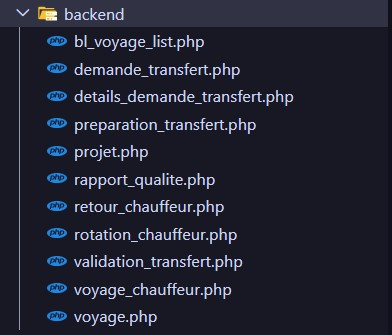
\includegraphics[width=0.75\textwidth]{assets/backend-tree.jpg}
    }{
    \textit{Arborescence du backend : fichier assets/backend-tree.jpg non trouvé.}
    }
    \caption{Arborescence des fichiers du backend}
    \label{fig:backend-tree}
    \end{figure}

    Chaque fichier du backend suit un schéma cohérent : il identifie la méthode HTTP (GET, POST, PUT, DELETE), extrait les paramètres de la requête, exécute les requêtes SQL nécessaires via \texttt{mysqli}, et retourne une réponse JSON structurée avec un champ \texttt{status} (booléen), un champ \texttt{message} et un champ \texttt{data}. Les opérations sensibles utilisent une transaction MySQL (\texttt{begin\_transaction}, \texttt{commit}, \texttt{rollback}) pour garantir l'intégrité des données.

    \subsection{Architecture du frontend : séparation par couches et par domaine}

    Le frontend adopte une \textbf{architecture en couches} avec une séparation claire des responsabilités, complétée par un alignement sur les domaines métier au sein de chaque couche. Cette organisation permet de développer, tester et maintenir chaque module de manière autonome tout en conservant une structure cohérente à l'échelle de l'application.

    Les couches sont les suivantes :
    \begin{itemize}[leftmargin=1.2em]
    \item \textbf{app/} (navigation) : routage basé sur les fichiers via Expo Router. Chaque route est un composant minimal qui délègue l'affichage à un écran dédié.
    \item \textbf{screens/} (présentation) : composants de page complets, contenant la logique d'affichage, les appels API via React Query et la gestion des interactions utilisateur.
    \item \textbf{components/} (composants réutilisables) : cartes de liste, feuilles de sélection (bottom sheets), boutons et indicateurs partagés entre les écrans.
    \item \textbf{api/} (accès aux données) : un fichier par domaine métier (voyage, retour, rapport qualité, etc.), exportant des fonctions typées qui appellent le client HTTP centralisé.
    \item \textbf{stores/} (état client) : états Zustand pour les formulaires multi-étapes, les bottom sheets et les sélections temporaires.
    \item \textbf{constants/} (infrastructure) : client HTTP centralisé, configuration React Query, thème et fonctions de permissions.
    \item \textbf{types/} (types partagés) : définitions TypeScript pour les entités communes (utilisateur, BL, dépôt, etc.).
    \end{itemize}

    Au sein de chaque couche, les fichiers sont nommés par domaine métier — par exemple \texttt{voyage.api.ts}, \texttt{VoyagesScreen.tsx}, \texttt{voyage.store.ts} — ce qui facilite la navigation et la maintenance. La gestion d'état suit une stratégie duale : React Query pour l'état serveur (données issues de l'API, avec cache et invalidation automatique) et Zustand pour l'état client (sélections, formulaires, modales).

    La Figure~\ref{fig:frontend-tree} présente l'arborescence des dossiers du frontend, illustrant la séparation par couches et par domaine.

    \begin{figure}[H]
    \centering
    \IfFileExists{assets/frontend-tree.jpg}{
    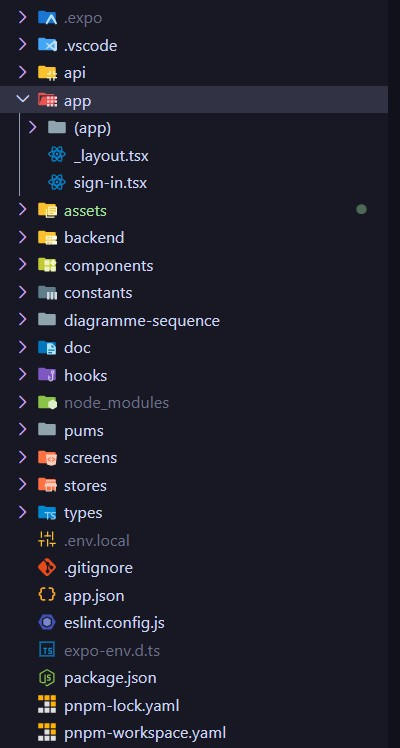
\includegraphics[width=0.75\textwidth]{assets/frontend-tree.jpg}
    }{
    \textit{Arborescence du frontend : fichier assets/frontend-tree.jpg non trouvé.}
    }
    \caption{Arborescence des dossiers du frontend}
    \label{fig:frontend-tree}
    \end{figure}

    \section{GitHub : Versionnement du code source}

    Tout le code source de l'application — frontend (React Native/Expo/TypeScript) et backend (PHP) — est hébergé dans un dépôt unique sur GitHub. Cette organisation monorepo facilite la cohérence entre le client et le serveur, le suivi des modifications et la collaboration. Chaque jour de développement, les modifications réalisées sont poussées via des commits réguliers intégrant les nouvelles fonctionnalités, les corrections de bugs et les améliorations progressives.

    La Figure~\ref{fig:github-repo} présente une capture d'écran du dépôt GitHub illustrant l'arborescence du projet et l'historique des commits.

    \begin{figure}[ht]
    \centering
    \IfFileExists{assets/github-repo.png}{
    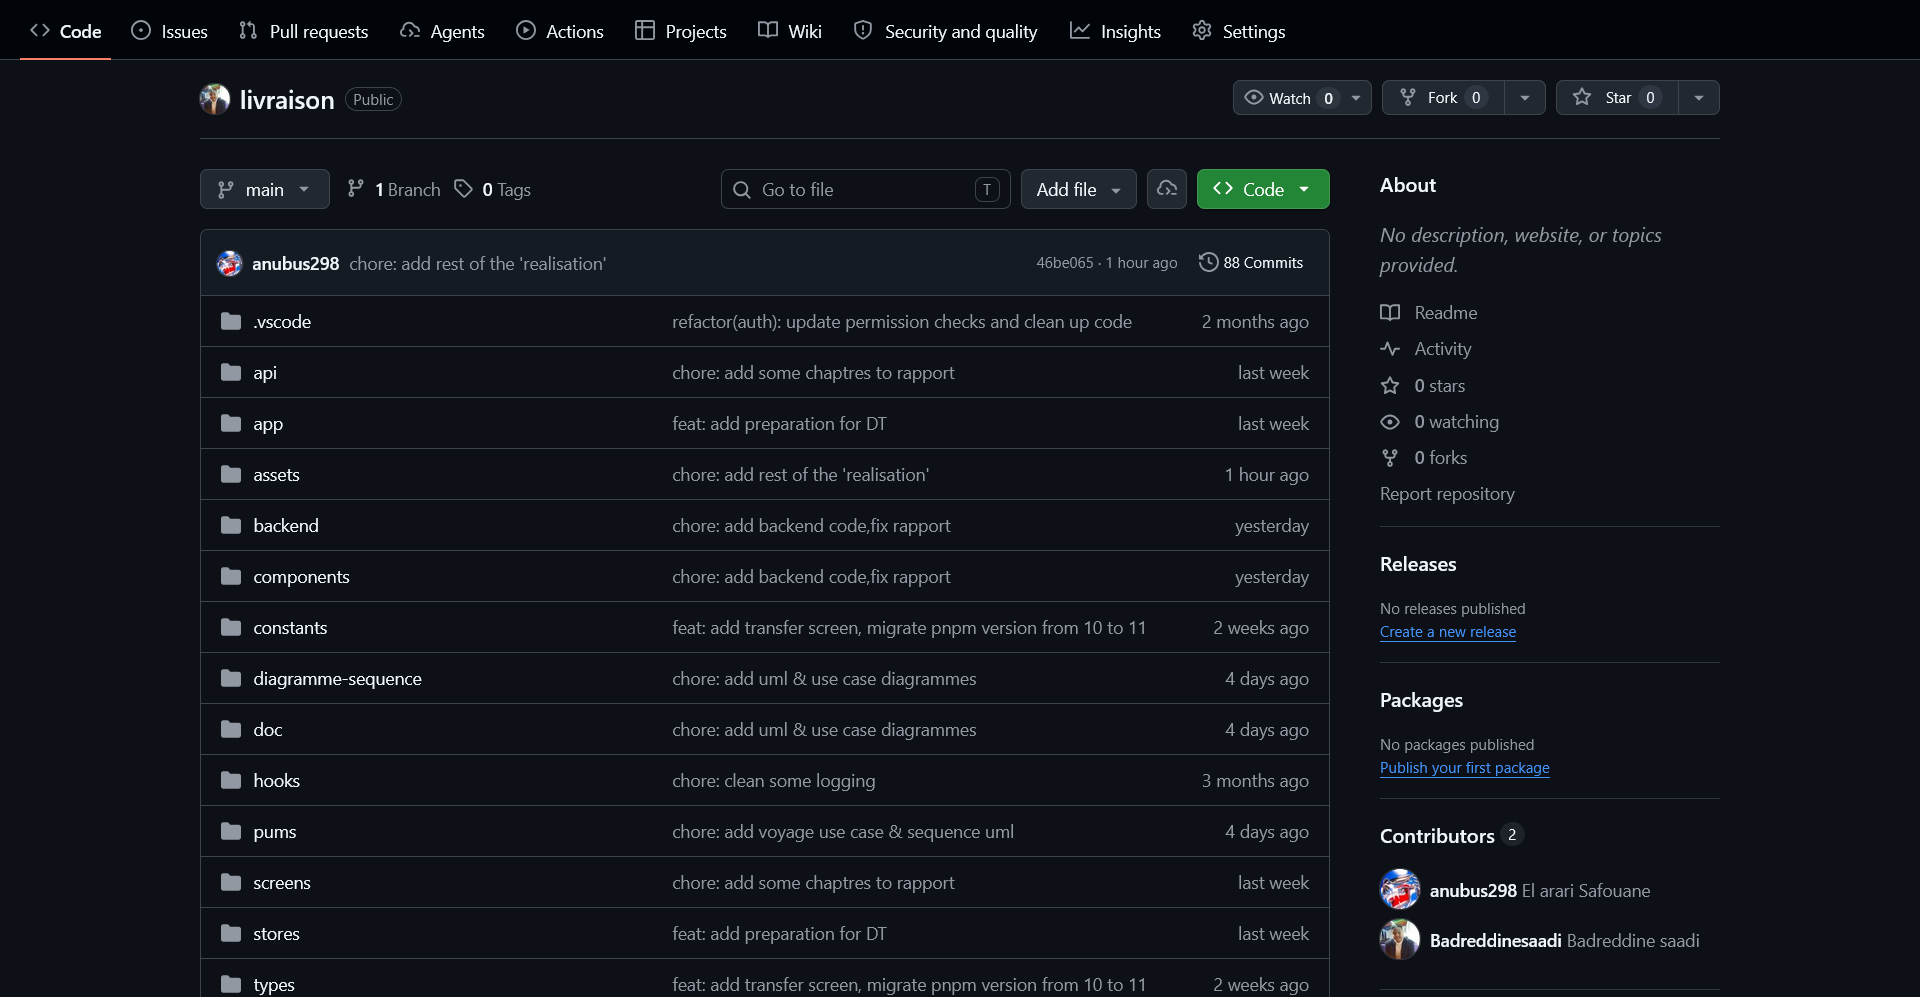
\includegraphics[width=0.75\textwidth]{assets/github-repo.png}
    }{
    \textit{Dépôt GitHub : fichier assets/github-repo.png non trouvé.}
    }
    \caption{Dépôt GitHub — arborescence du projet frontend et backend}
    \label{fig:github-repo}
    \end{figure}

    \section{Réalisation des sprints de l'application}

    Cette section décrit la réalisation concrète de l'application, sprint par sprint. Le Sprint 1 ayant été consacré à l'initialisation du boilerplate, à la mise en place du design system et à l'autoformation sur les technologies, le démarrage effectif du développement intervient au Sprint 2, qui constitue le point d'entrée de la réalisation.

    \subsection{Sprint 2 : Authentification et module Voyages}

    \subsubsection{Authentification}

    L'authentification repose sur un mécanisme de jetons (\textit{token-based authentication}) de type stateful : à la connexion, le backend vérifie les identifiants de l'utilisateur dans la base de données, génère un jeton unique associé à la session, et le renvoie au client. Ce jeton est stocké de manière sécurisée sur le terminal mobile via \texttt{expo-secure-store} et transmis dans l'en-tête \texttt{auth\_token} de chaque requête API ultérieure. Le backend valide systématiquement le jeton avant d'exécuter toute opération, garantissant ainsi que seuls les utilisateurs authentifiés accèdent aux endpoints protégés.

    La Figure~\ref{fig:auth-flow-uml} présente le diagramme de séquence du flux d'authentification, détaillant les échanges entre le client mobile, le backend et la base de données.

    \begin{figure}[H]
    \centering
    \IfFileExists{assets/auth-flow-uml.png}{
    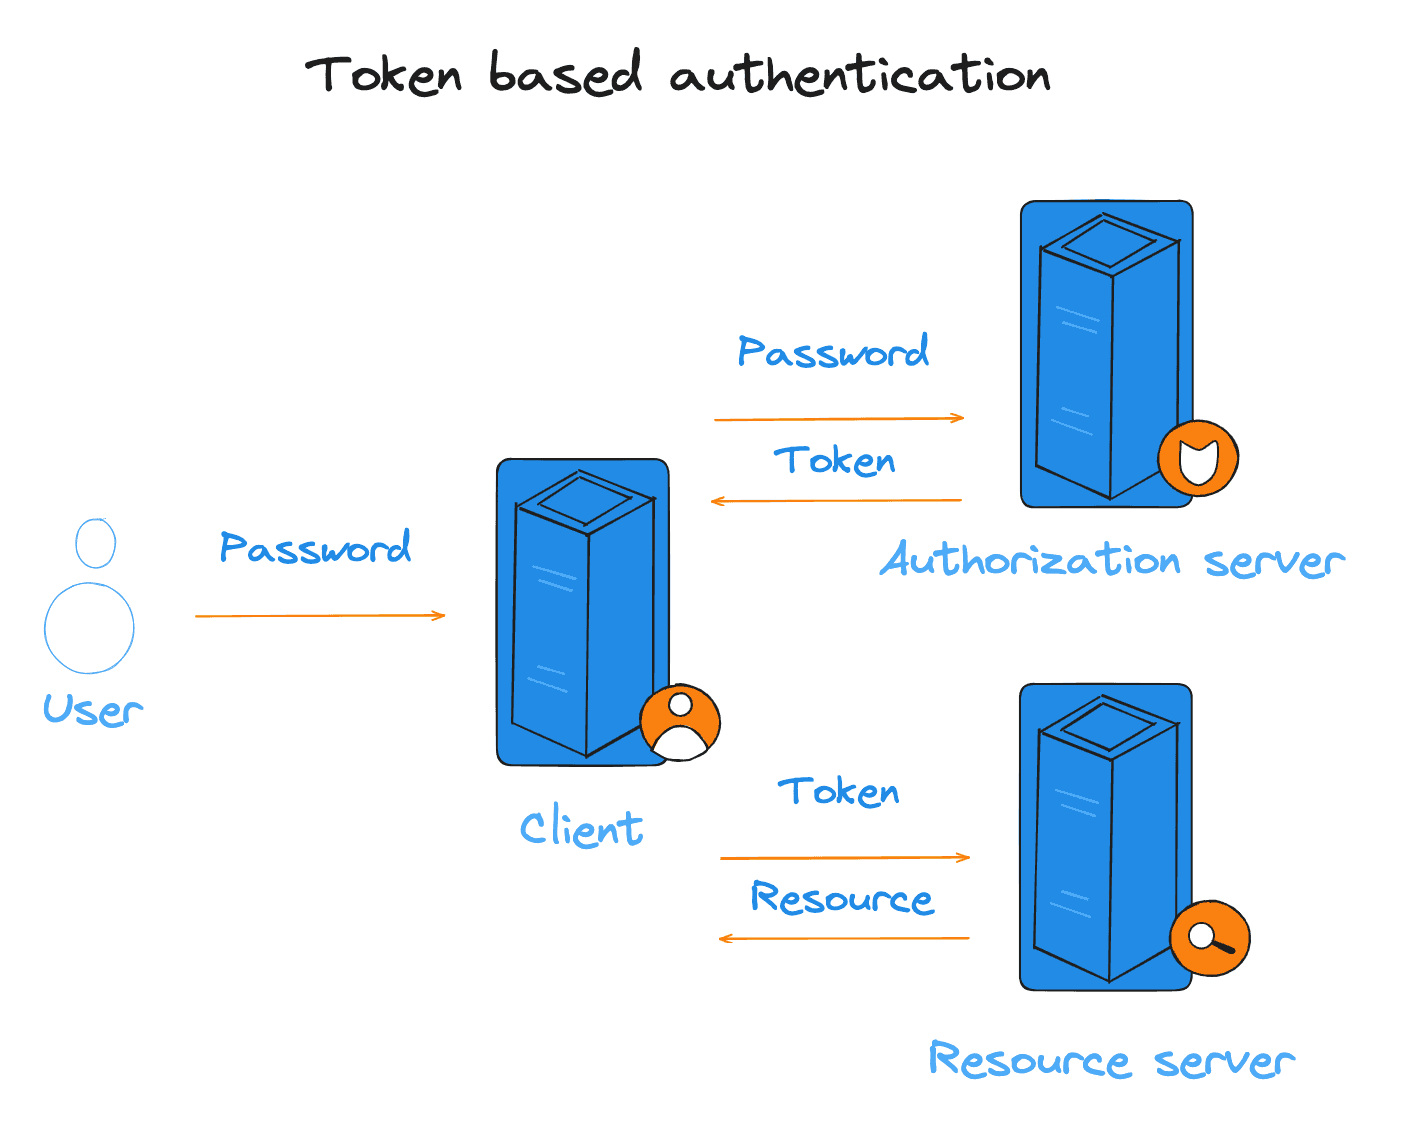
\includegraphics[width=0.8\textwidth]{assets/auth-flow-uml.png}
    }{
    \textit{Diagramme du flux d'authentification : fichier assets/auth-flow-uml.png non trouvé.}
    }
    \caption{Diagramme de séquence — Flux d'authentification}
    \label{fig:auth-flow-uml}
    \end{figure}

    La Figure~\ref{fig:login-screen} présente l'interface de connexion et la Figure~\ref{fig:login-fail} illustre l'échec d'authentification.

    \begin{figure}[ht]
    \centering
    \begin{minipage}[b]{0.4\textwidth}
    \centering
    \IfFileExists{assets/login-screen.jpeg}{
    
\includegraphics[width=0.8\textwidth]{assets/login-screen.jpeg}
    }{
    \textit{Écran de connexion : fichier assets/login-screen.jpeg non trouvé.}
    }
    \caption{Interface de connexion}
    \label{fig:login-screen}
    \end{minipage}\hfill
    \begin{minipage}[b]{0.4\textwidth}
    \centering
    \IfFileExists{assets/login-fail.jpg}{
    
\includegraphics[width=0.8\textwidth]{assets/login-fail.jpg}
    }{
    \textit{Échec de connexion : fichier assets/login-fail.jpg non trouvé.}
    }
    \caption{Échec d'authentification}
    \label{fig:login-fail}
    \end{minipage}
    \end{figure}

    \subsubsection{Écran d'accueil}

    Après une authentification réussie, l'utilisateur accède à l'écran d'accueil. Celui-ci affiche une grille de modules disponibles — Voyages, Retours chauffeur, Rapports qualité, Rotation chauffeur, Lieux de projets et Demandes de transfert — sous forme de cartes cliquables. Chaque carte n'est visible que si l'utilisateur dispose de la permission correspondante. Cette logique est pilotée par les fonctions de permission définies dans \texttt{constants/permissions.ts} : avant le rendu de chaque carte, une vérification du type \texttt{canAccessVoyageModule(user)} détermine son affichage.

    Dans la barre d'en-tête, une icône utilisateur est placée en haut à gauche. Lorsqu'elle est pressée, un menu latéral (drawer) se déploie depuis le bord gauche de l'écran. Ce drawer liste les modules autorisés pour l'utilisateur connecté, reprenant la même logique de permission que l'écran d'accueil, et propose en bas du menu un bouton de déconnexion. La déconnexion supprime le jeton d'authentification du stockage sécurisé et redirige l'utilisateur vers l'écran de connexion.

    La Figure~\ref{fig:home-screen} présente l'écran d'accueil avec les modules disponibles pour un utilisateur donné, et la Figure~\ref{fig:drawer-menu} illustre le drawer déployé.

    \begin{figure}[ht]
    \centering
    \begin{minipage}[b]{0.4\textwidth}
    \centering
    \IfFileExists{assets/home-screen.jpg}{
    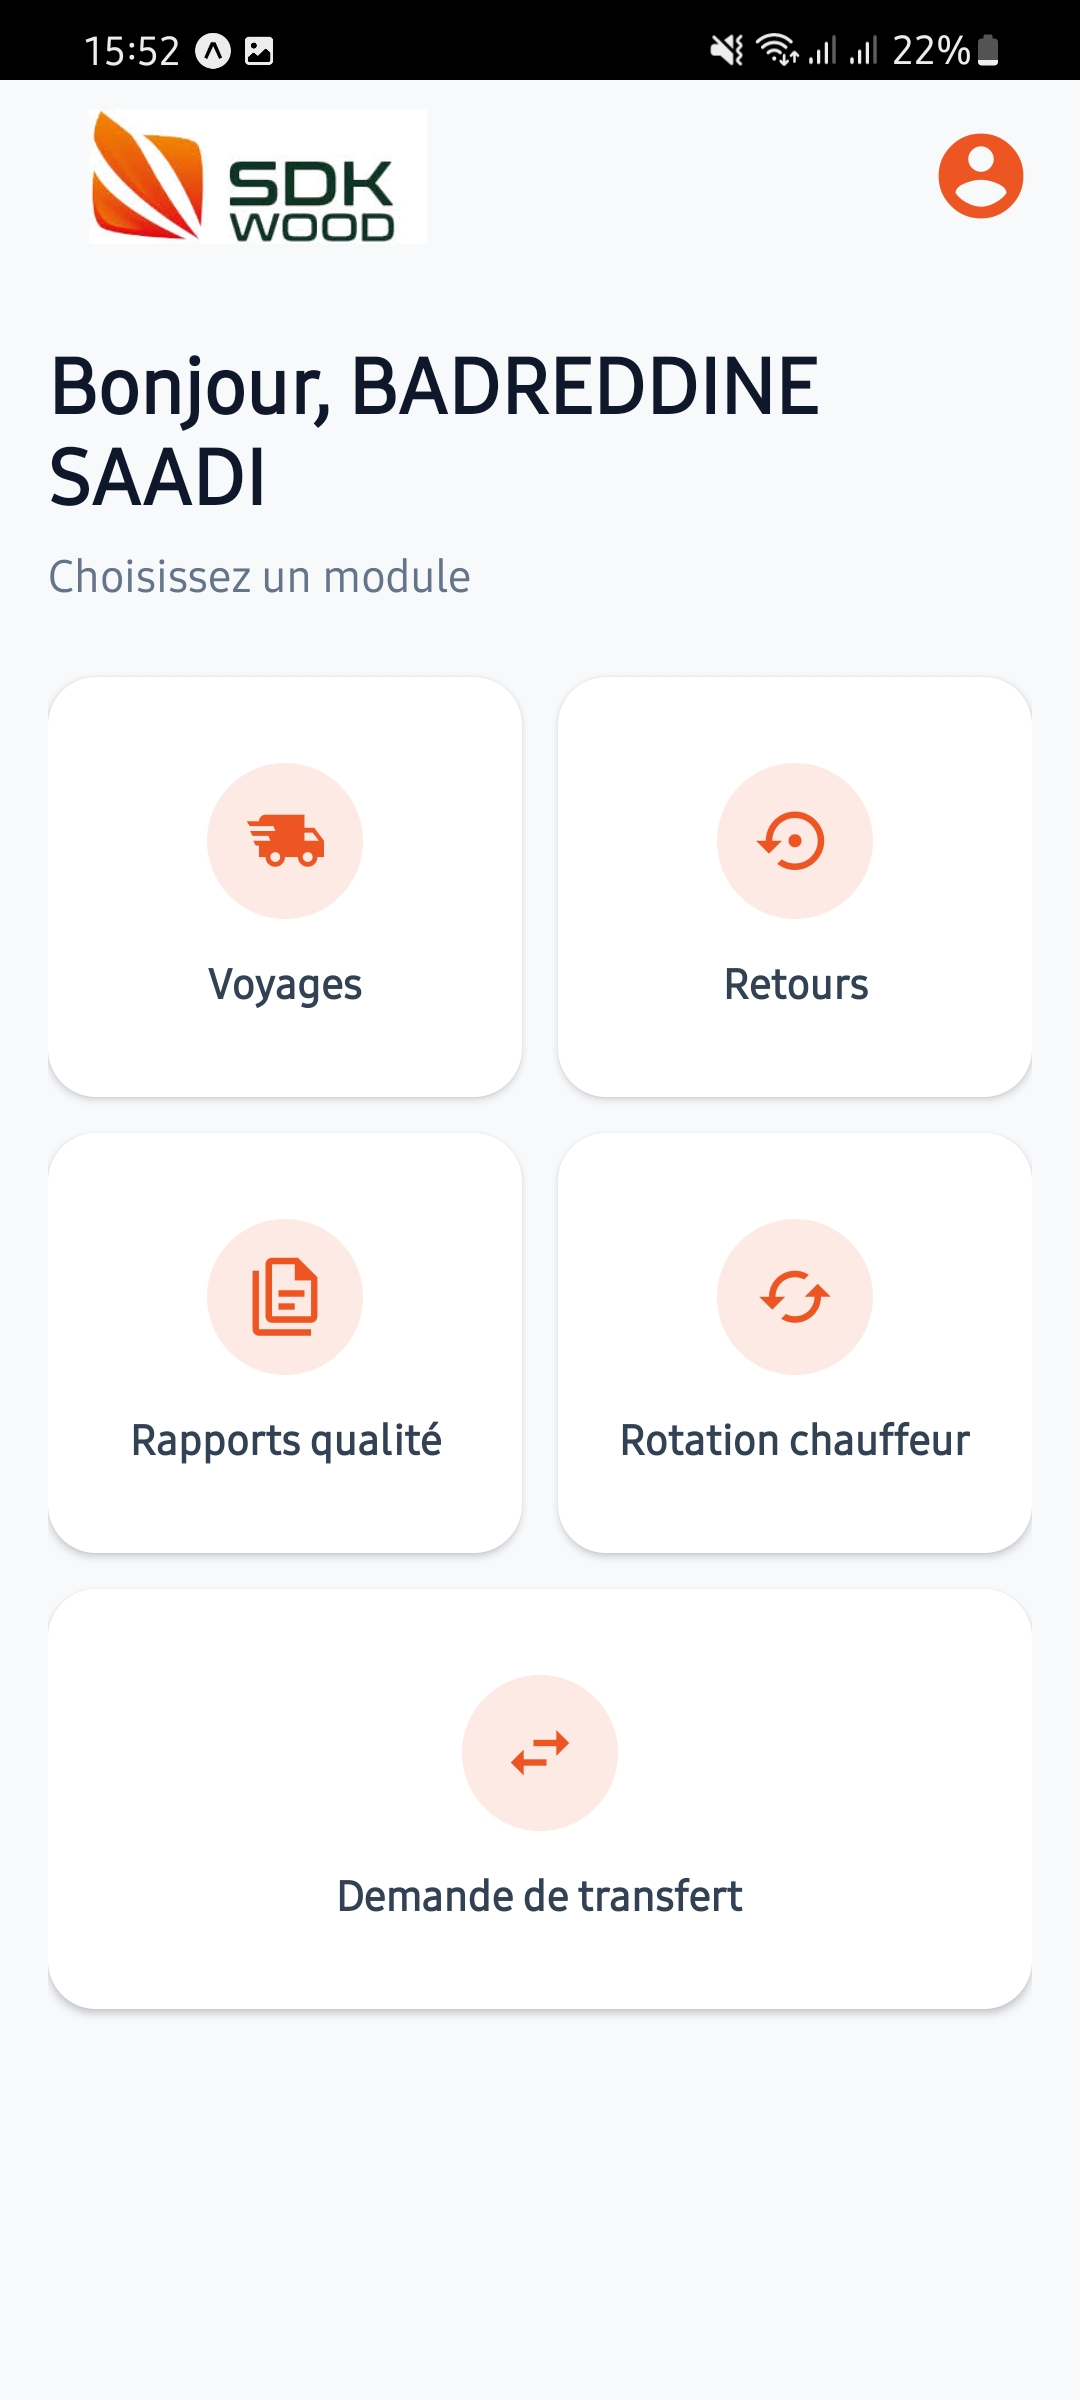
\includegraphics[width=0.8\textwidth]{assets/home-screen.jpg}
    }{
    \textit{Écran d'accueil : fichier assets/home-screen.jpg non trouvé.}
    }
    \caption{Écran d'accueil avec les modules}
    \label{fig:home-screen}
    \end{minipage}\hfill
    \begin{minipage}[b]{0.4\textwidth}
    \centering
    \IfFileExists{assets/drawer-menu.jpg}{
    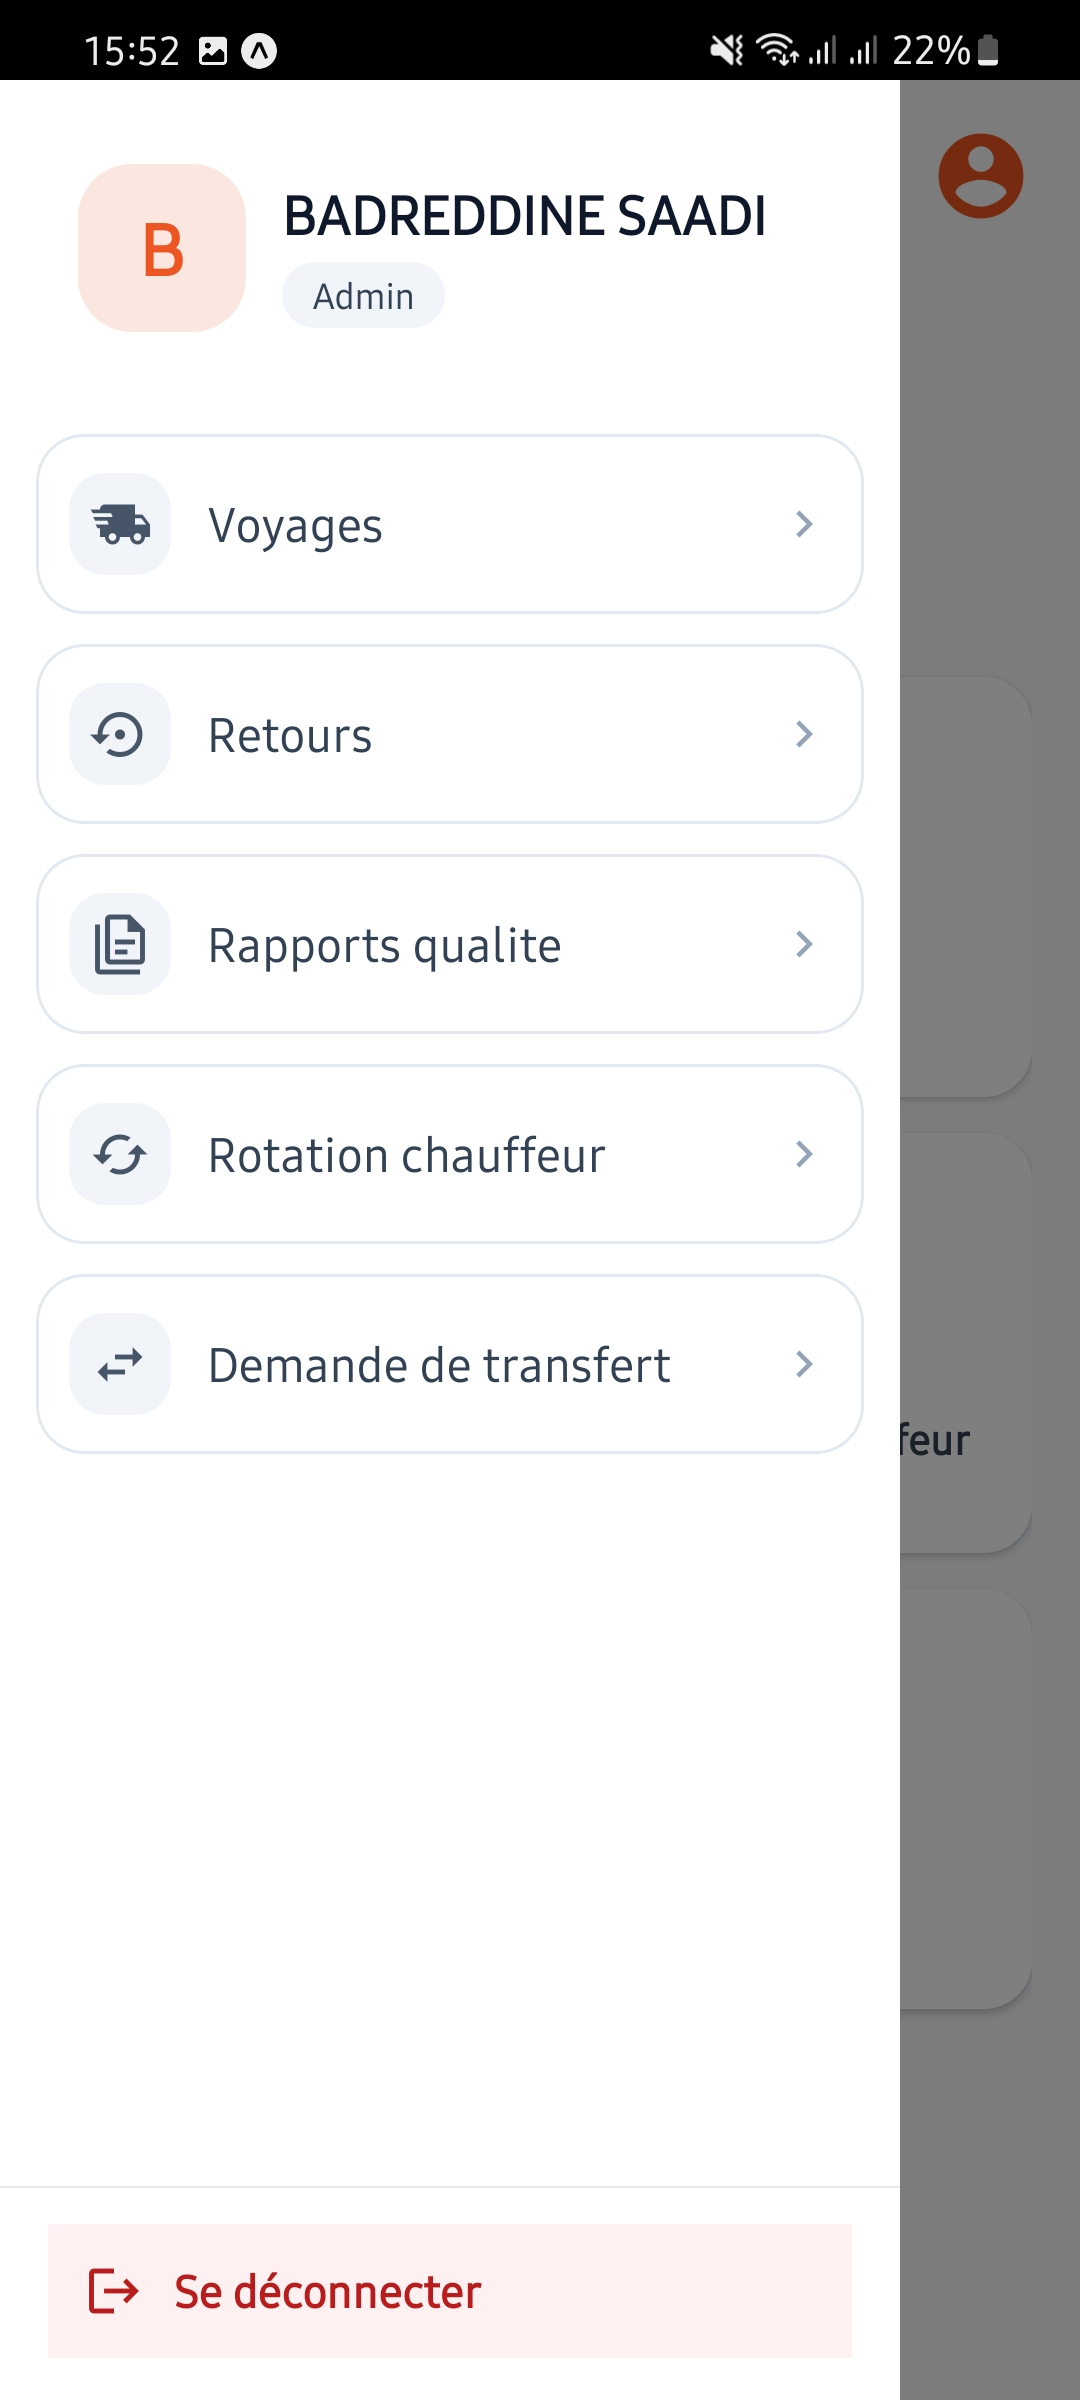
\includegraphics[width=0.8\textwidth]{assets/drawer-menu.jpg}
    }{
    \textit{Drawer : fichier assets/drawer-menu.jpg non trouvé.}
    }
    \caption{Drawer latéral avec les modules et la déconnexion}
    \label{fig:drawer-menu}
    \end{minipage}
    \end{figure}

    \subsubsection{Module Voyages}

    L'écran principal affiche la liste paginée des voyages sous forme de cartes, avec l'identifiant, le chauffeur, les bons de livraison (BL) et un badge de statut coloré. Un bouton de création placé en haut à droite permet d'initier un voyage en trois étapes : informations du voyage, sélection des BL avec photo obligatoire, et récapitulatif avant confirmation. La carte est expansible et dévoile des informations supplémentaires ainsi que, selon le rôle, jusqu'à cinq actions :

    \begin{itemize}[leftmargin=1.2em]
    \item \textbf{Modifier} : réservé à l'agent de livraison. Ouvre une feuille modale permettant de changer le chauffeur, le véhicule, le dépôt, la ville ou la liste des BL associés.
    \item \textbf{Clôturer BL} : réservé au chauffeur. Ouvre une feuille modale listant les BL non encore clôturés du voyage. L'utilisateur sélectionne un BL, ce qui le redirige vers un écran de prise de photo en direct depuis l'appareil photo du terminal mobile. La photo capture les produits physiques livrés comme preuve ; une fois la photo prise, la clôture est confirmée et le BL passe au statut \og Livré \fg.
    \item \textbf{Achever} : réservé à l'agent de livraison. Ouvre une feuille de confirmation avec trois champs obligatoires : le kilométrage réel du véhicule au retour, la date de retour et l'heure de retour. La validation de cette feuille marque le voyage comme achevé.
    \item \textbf{Voir les détails} : ouvre l'écran de détail du voyage, qui affiche les informations complètes du voyage, la liste des BL avec leur statut et les clichés photographiques pris lors de la clôture de chaque BL.
    \item \textbf{Supprimer} : réservé à l'agent de livraison. Ouvre une feuille de confirmation demandant de valider la suppression définitive du voyage.
    \end{itemize}

    La barre de recherche en haut de l'écran permet de filtrer les voyages par identifiant, par nom de chauffeur ou par client associé aux BL.

    La Figure~\ref{fig:voyage-list} montre la liste des voyages avec le bouton de création en haut à droite, et les Figures~\ref{fig:voyage-expanded} et~\ref{fig:voyage-sheet} illustrent respectivement l'expansion d'une carte et la feuille d'actions.

    La Figure~\ref{fig:voyage-create-step1}, la Figure~\ref{fig:voyage-create-step2} et la Figure~\ref{fig:voyage-create-step3} illustrent les trois étapes de la création d'un voyage : saisie des informations, sélection des BL, et récapitulatif avant confirmation. Les Figures~\ref{fig:voyage-cloturer-sheet} et~\ref{fig:voyage-cloturer-photo} détaillent le flux de clôture d'un BL.

    \begin{figure}[H]
    \centering
    \IfFileExists{assets/voyage-list.jpg}{
    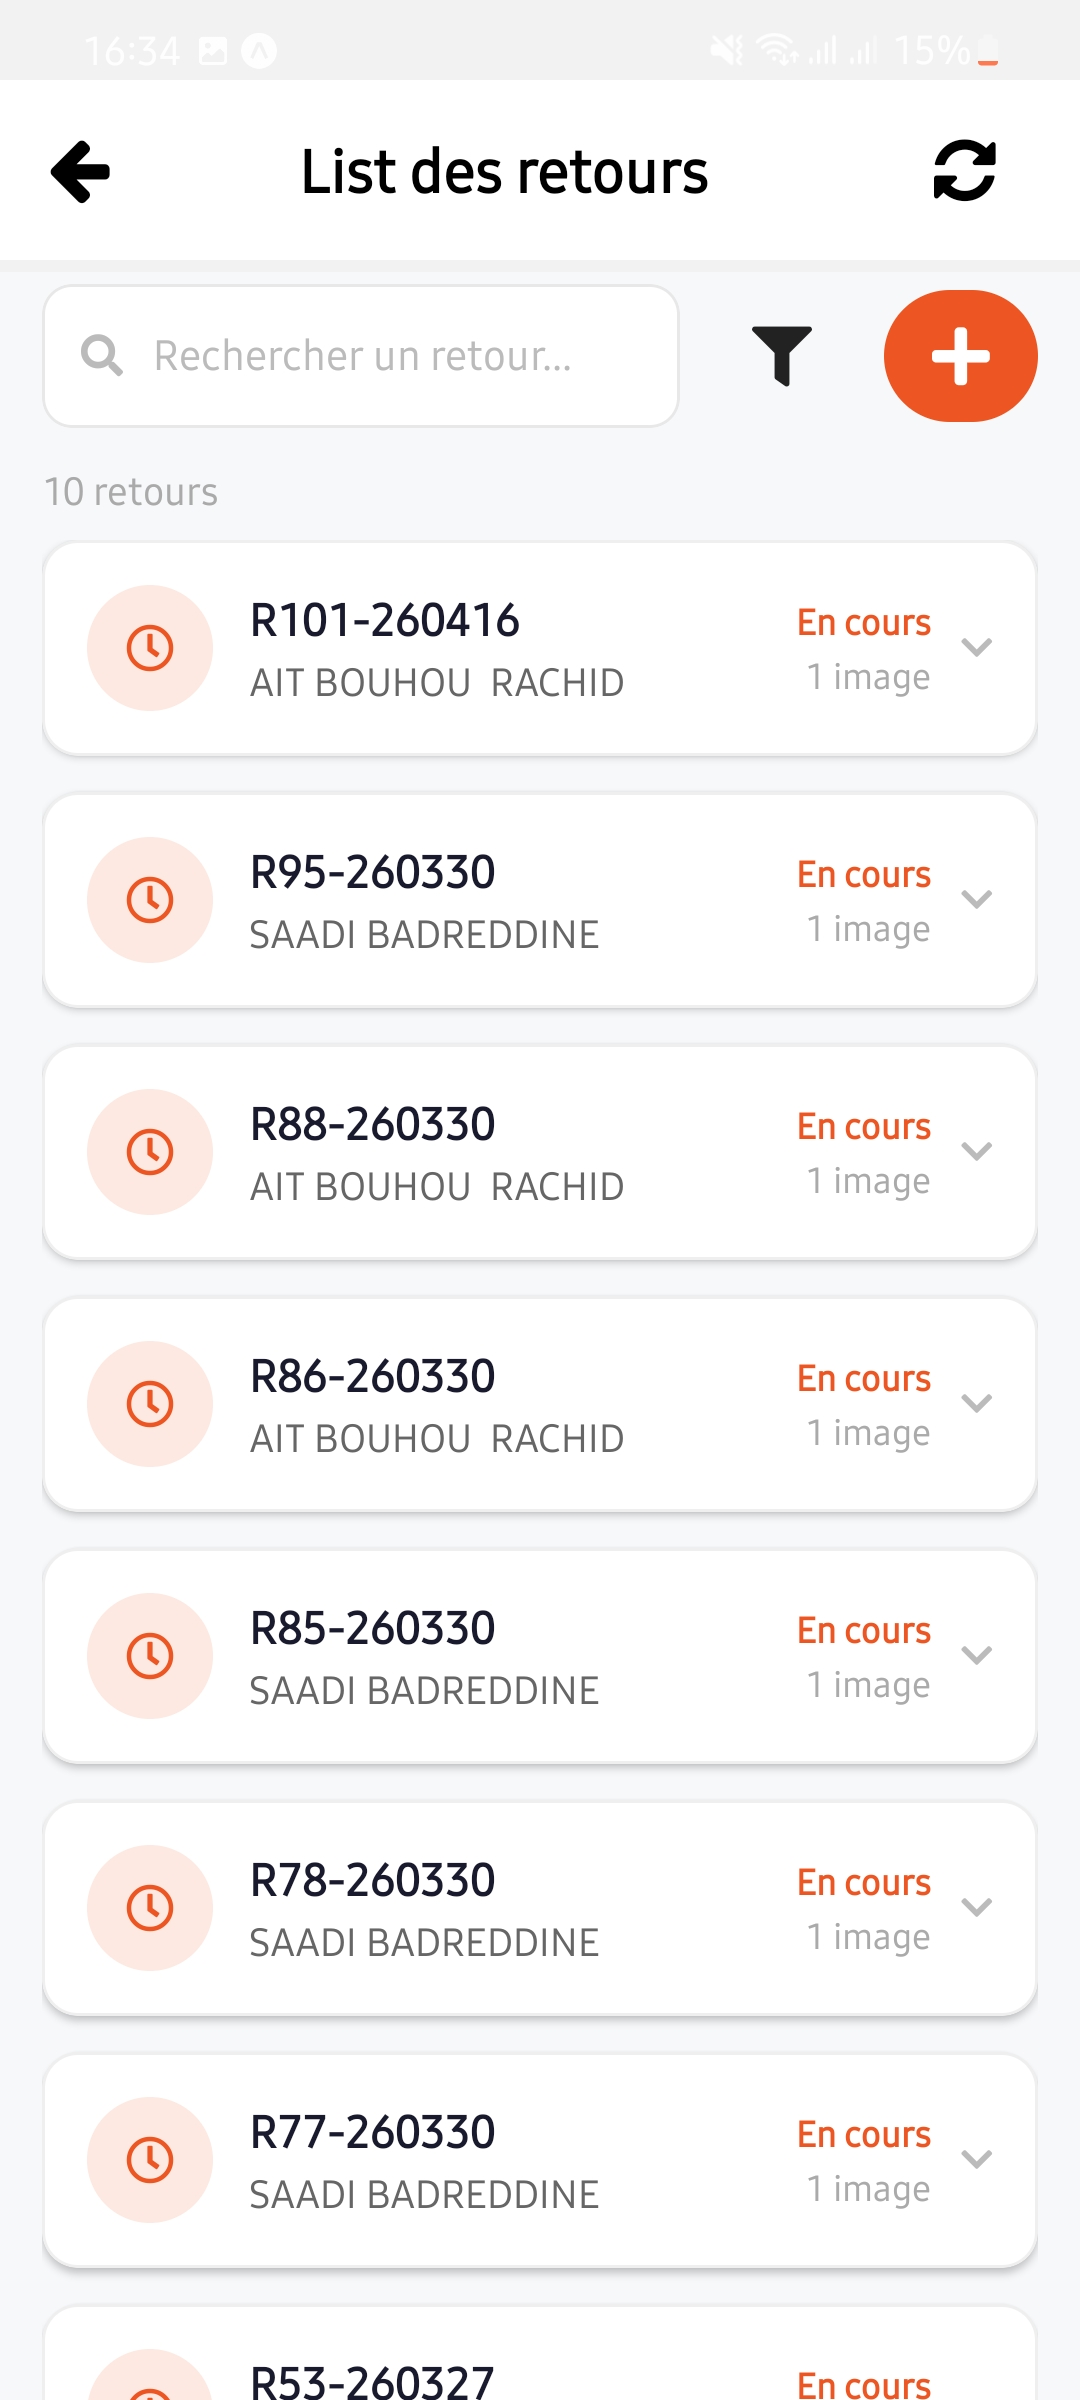
\includegraphics[width=0.35\textwidth]{assets/voyage-list.jpg}
    }{
    \textit{Liste des voyages : fichier assets/voyage-list.jpg non trouvé.}
    }
    \caption{Liste des voyages — cartes avec BL et statuts}
    \label{fig:voyage-list}
    \end{figure}

    \begin{figure}[H]
    \centering
    \begin{minipage}[b]{0.45\textwidth}
    \centering
    \IfFileExists{assets/voyage-card-expanded.jpg}{
    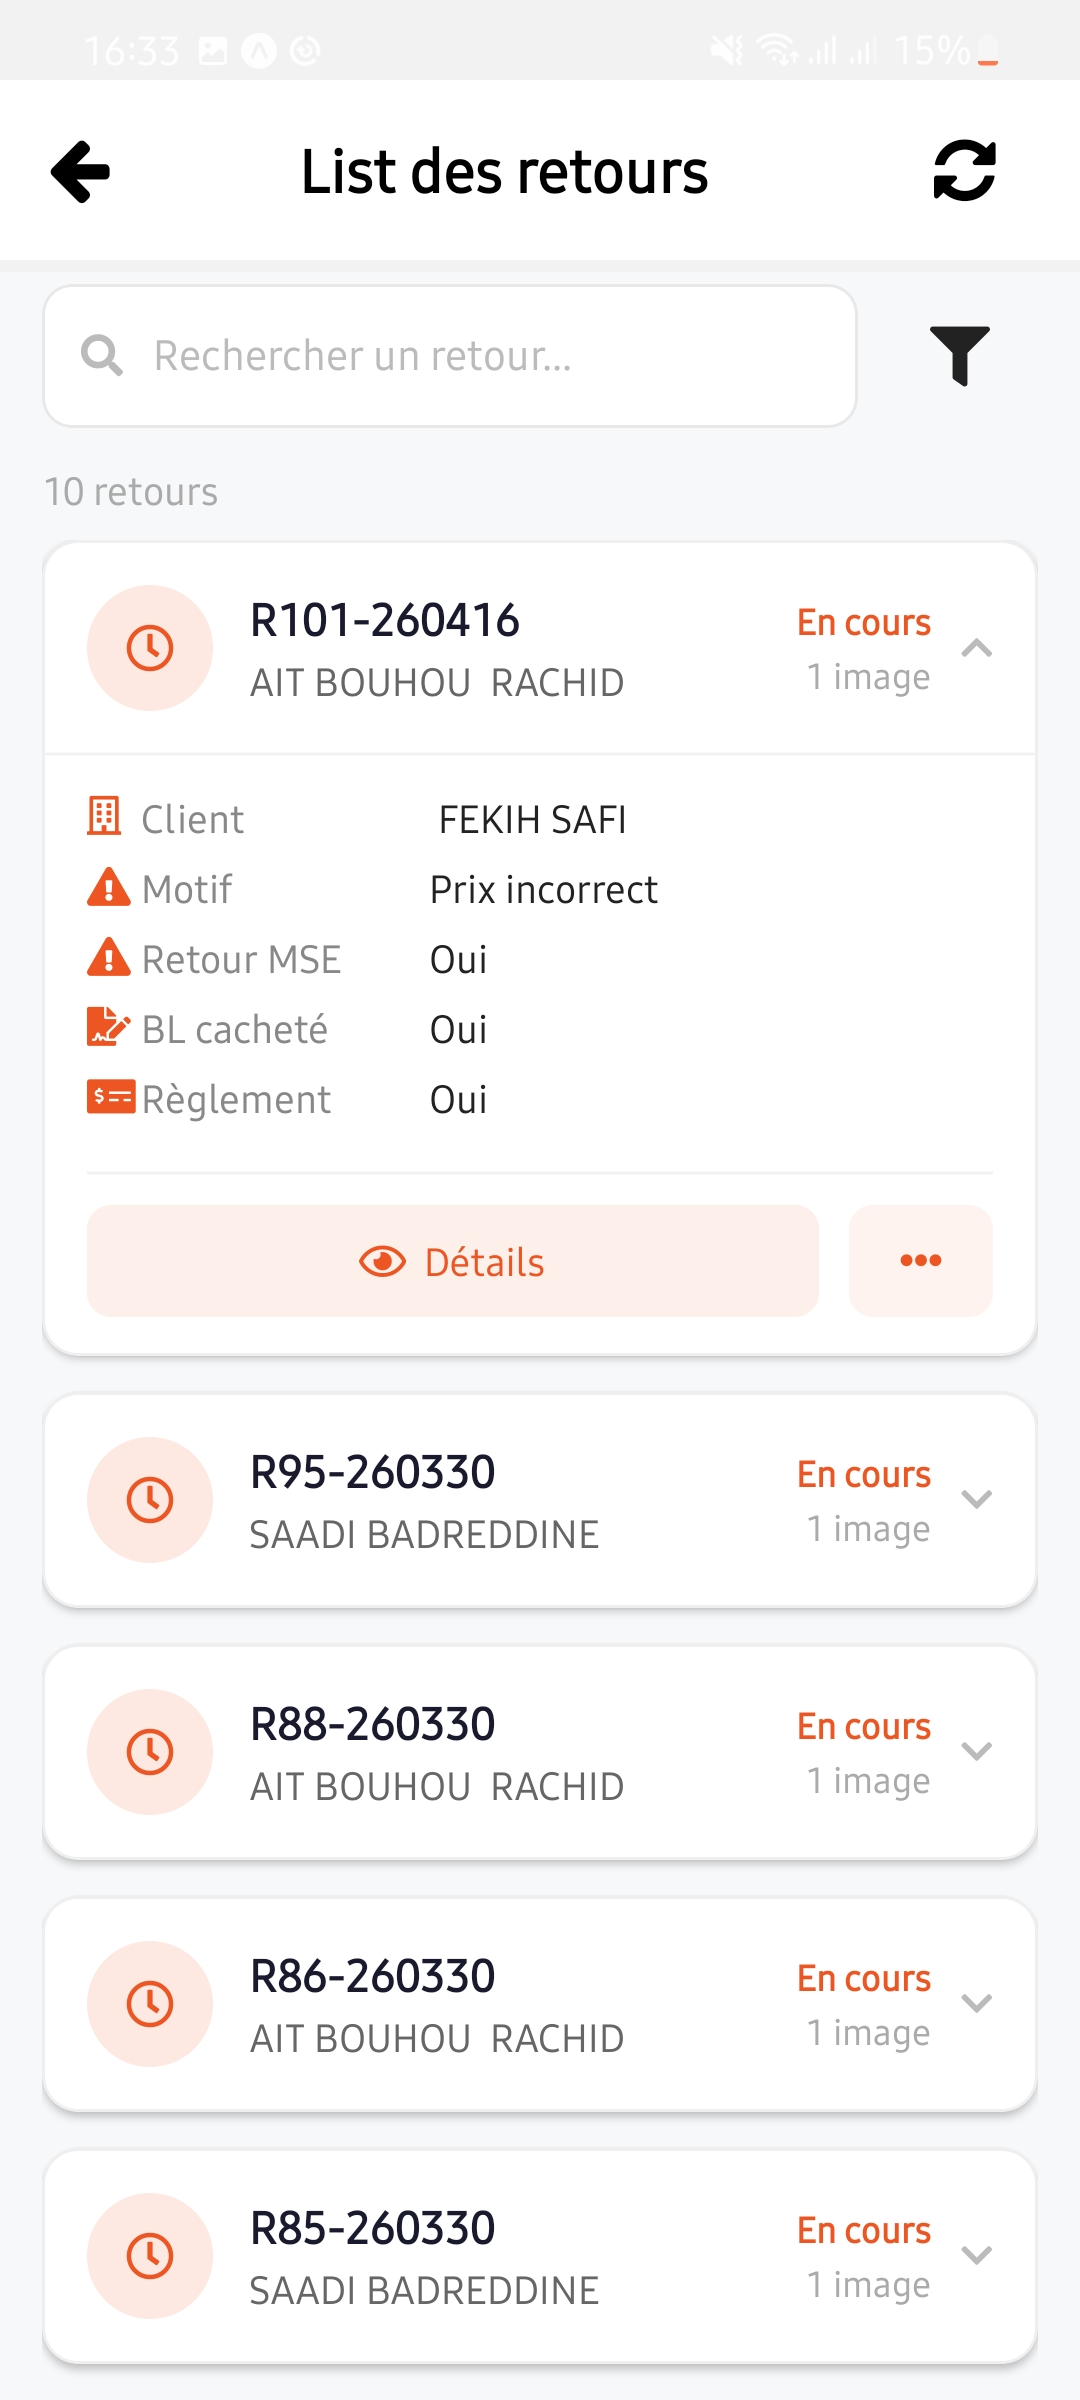
\includegraphics[width=0.9\textwidth]{assets/voyage-card-expanded.jpg}
    }{
    \textit{Carte expansée : fichier assets/voyage-card-expanded.jpg non trouvé.}
    }
    \caption{Carte de voyage expansée}
    \label{fig:voyage-expanded}
    \end{minipage}\hfill
    \begin{minipage}[b]{0.45\textwidth}
    \centering
    \IfFileExists{assets/voyage-bottom-sheet.jpg}{
    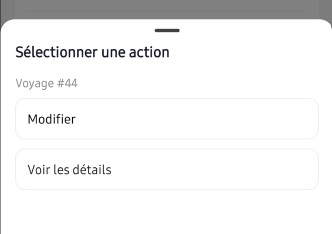
\includegraphics[width=0.9\textwidth]{assets/voyage-bottom-sheet.jpg}
    }{
    \textit{Feuille d'actions : fichier assets/voyage-bottom-sheet.jpg non trouvé.}
    }
    \caption{Feuille d'actions — Modifier / Voir les détails}
    \label{fig:voyage-sheet}
    \end{minipage}
    \end{figure}

    \begin{figure}[H]
    \centering
    \begin{minipage}[b]{0.32\textwidth}
    \centering
    \IfFileExists{assets/voyage-create-step1.jpg}{
    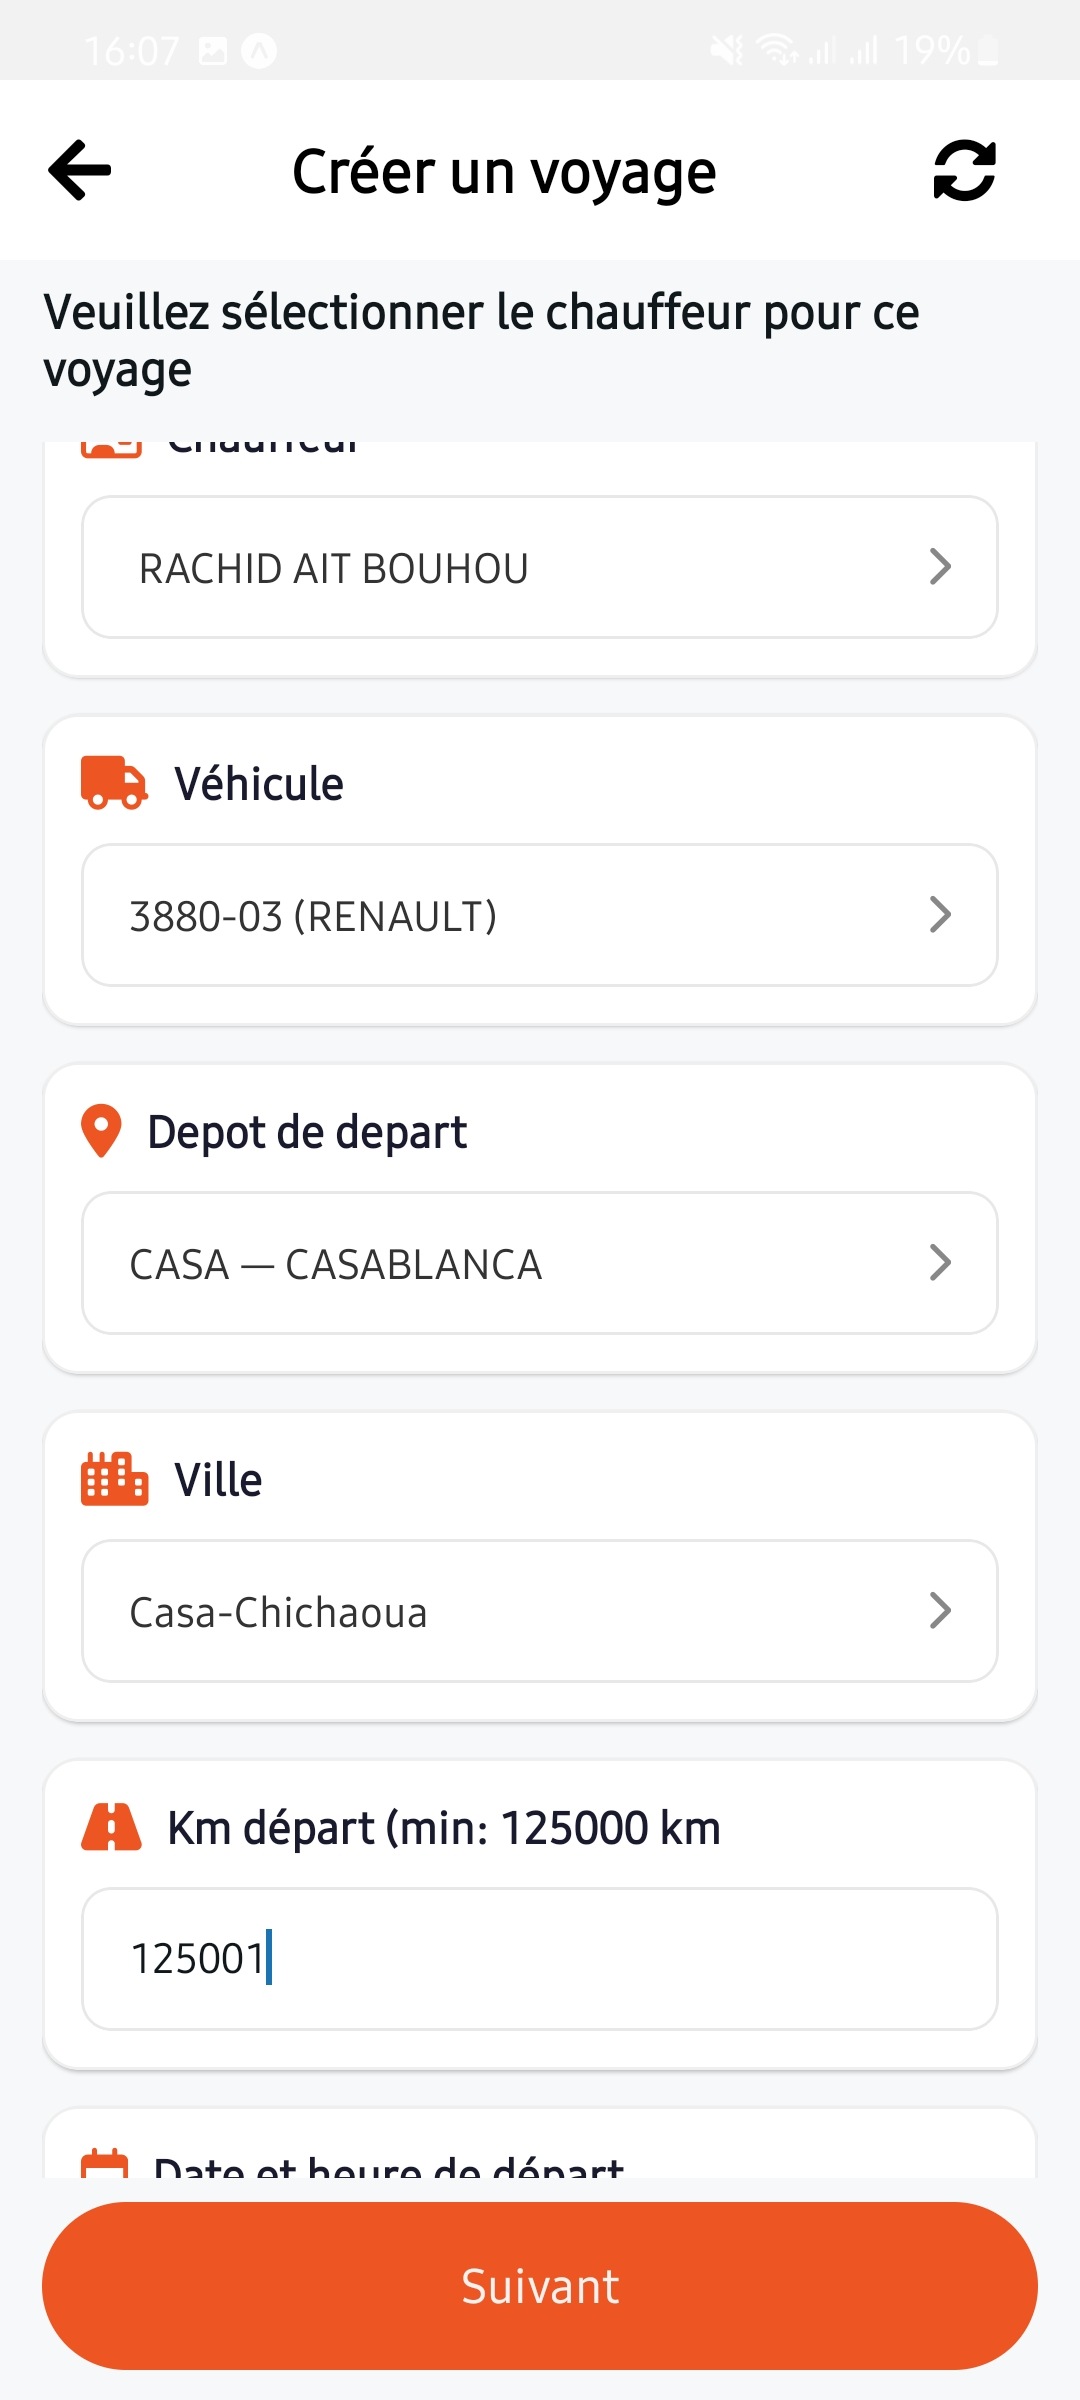
\includegraphics[width=\textwidth]{assets/voyage-create-step1.jpg}
    }{
    \textit{Étape 1 : fichier assets/voyage-create-step1.jpg non trouvé.}
    }
    \caption{Étape 1 — Saisie des informations}
    \label{fig:voyage-create-step1}
    \end{minipage}\hfill
    \begin{minipage}[b]{0.32\textwidth}
    \centering
    \IfFileExists{assets/voyage-create-step2.jpg}{
    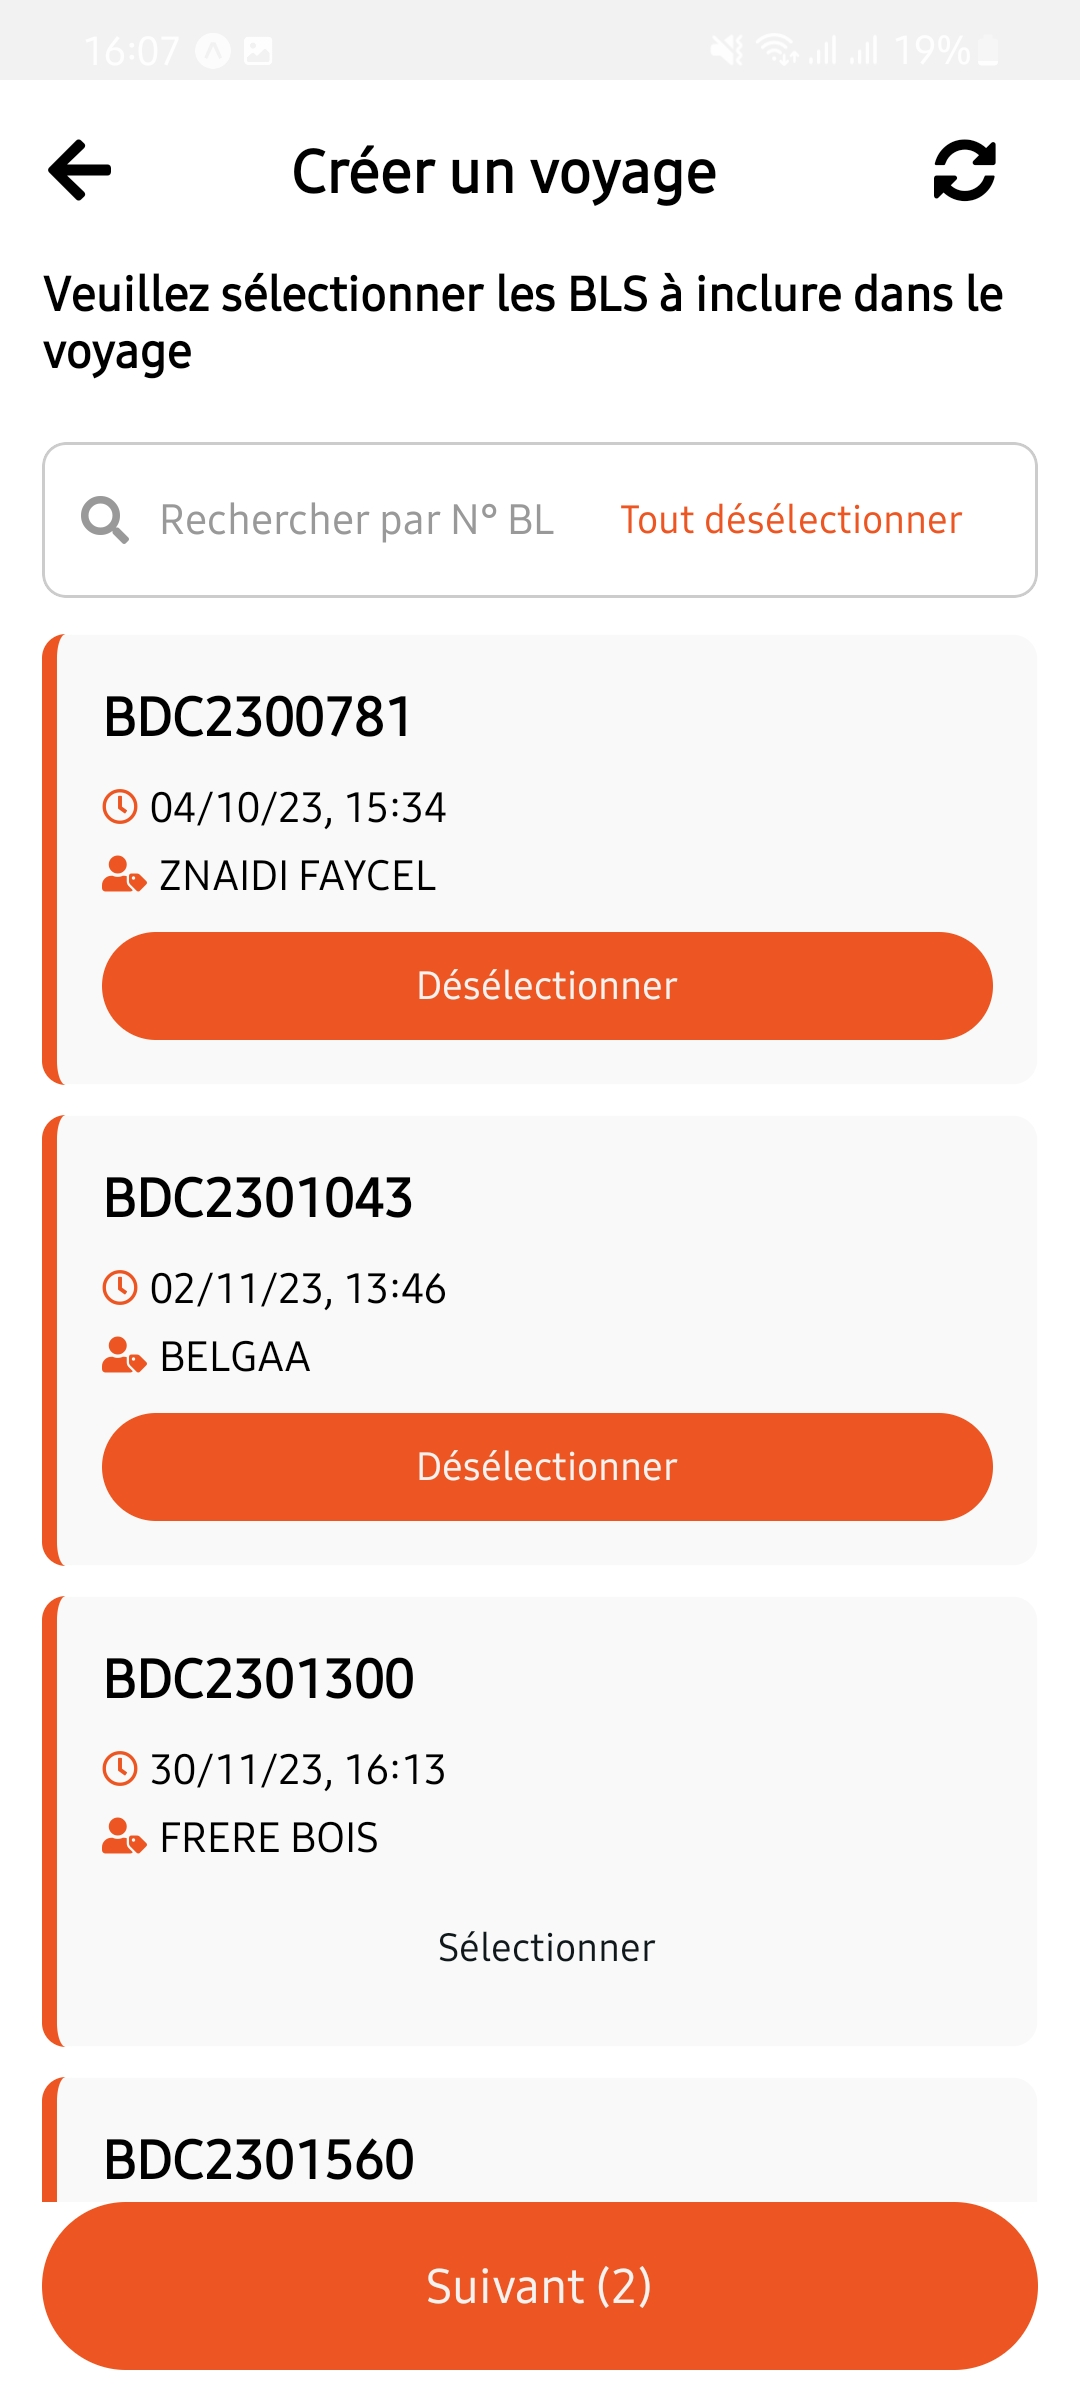
\includegraphics[width=\textwidth]{assets/voyage-create-step2.jpg}
    }{
    \textit{Étape 2 : fichier assets/voyage-create-step2.jpg non trouvé.}
    }
    \caption{Étape 2 — Sélection des BL}
    \label{fig:voyage-create-step2}
    \end{minipage}\hfill
    \begin{minipage}[b]{0.32\textwidth}
    \centering
    \IfFileExists{assets/voyage-create-step3.jpg}{
    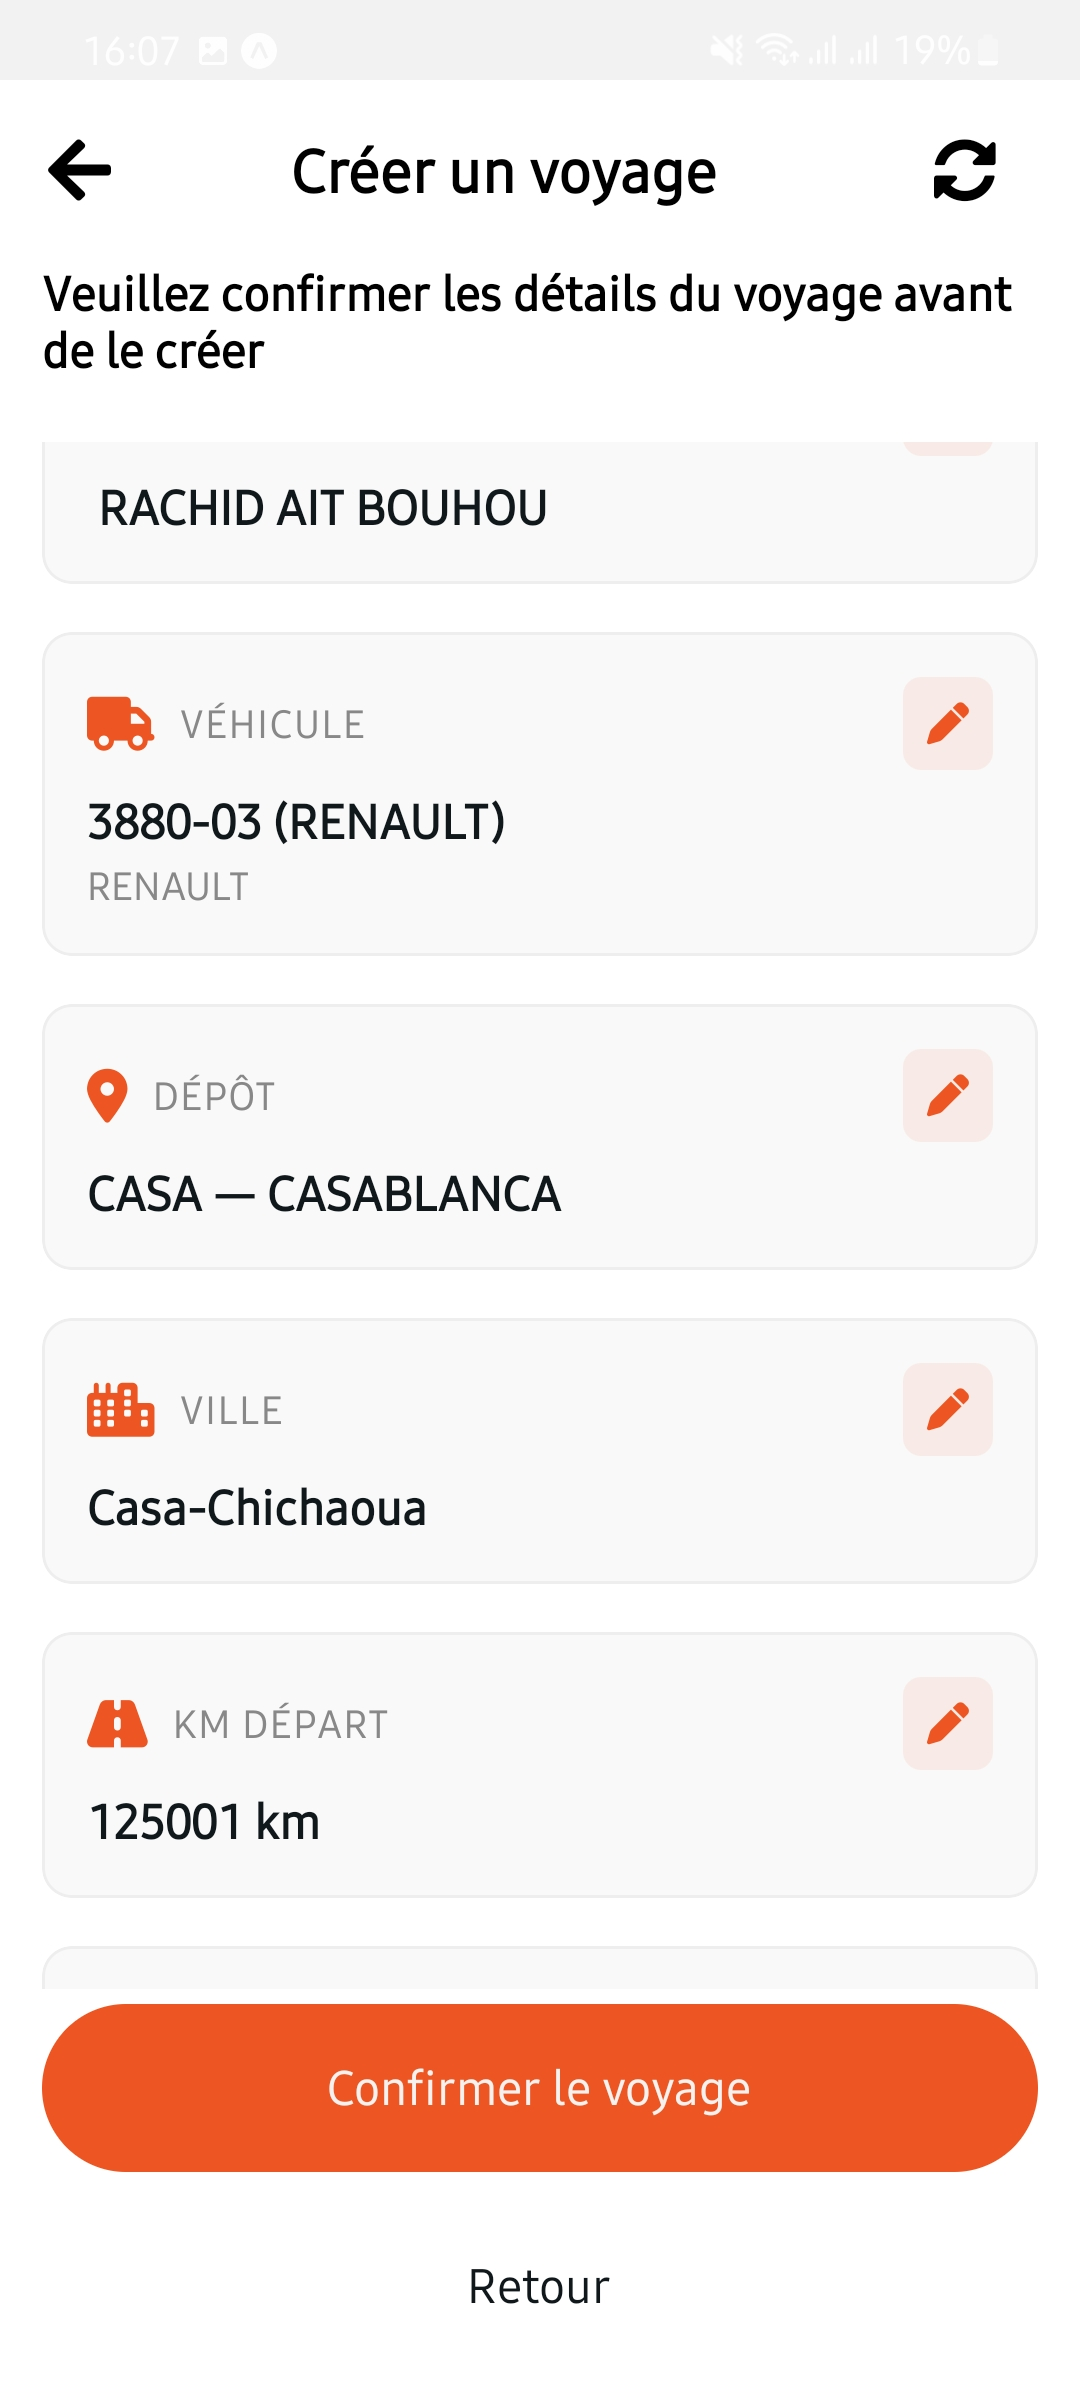
\includegraphics[width=\textwidth]{assets/voyage-create-step3.jpg}
    }{
    \textit{Étape 3 : fichier assets/voyage-create-step3.jpg non trouvé.}
    }
    \caption{Étape 3 — Récapitulatif et confirmation}
    \label{fig:voyage-create-step3}
    \end{minipage}
    \end{figure}

    \begin{figure}[H]
    \centering
    \begin{minipage}[b]{0.45\textwidth}
    \centering
    \IfFileExists{assets/voyage-cloturer-sheet.jpg}{
    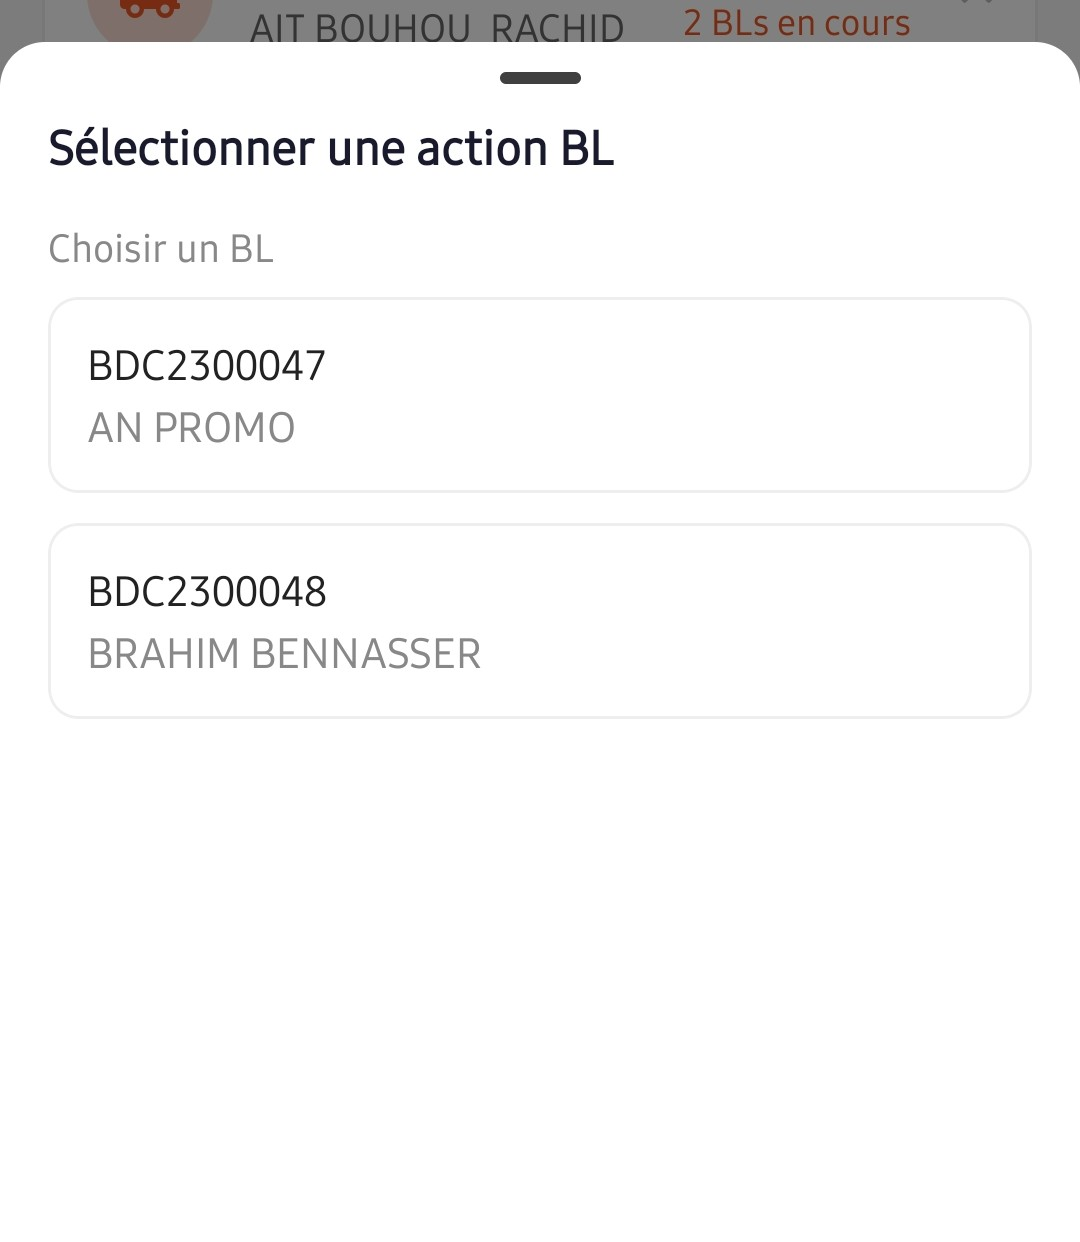
\includegraphics[width=0.9\textwidth]{assets/voyage-cloturer-sheet.jpg}
    }{
    \textit{Clôturer BL — sélection : fichier assets/voyage-cloturer-sheet.jpg non trouvé.}
    }
    \caption{Feuille de sélection des BL à clôturer}
    \label{fig:voyage-cloturer-sheet}
    \end{minipage}\hfill
    \begin{minipage}[b]{0.45\textwidth}
    \centering
    \IfFileExists{assets/voyage-cloturer-photo.jpg}{
    
\includegraphics[width=0.9\textwidth]{assets/voyage-cloturer-photo.jpg}
    }{
    \textit{Clôturer BL — photo : fichier assets/voyage-cloturer-photo.jpg non trouvé.}
    }
    \caption{Prise de photo de preuve du BL}
    \label{fig:voyage-cloturer-photo}
    \end{minipage}
    \end{figure}

    La Figure~\ref{fig:voyage-achever} présente la feuille d'achèvement d'un voyage, la Figure~\ref{fig:voyage-details} montre l'écran de détail avec les BL et leurs images, et la Figure~\ref{fig:voyage-delete-confirm} illustre la confirmation de suppression.

    \begin{figure}[H]
    \centering
    \begin{minipage}[b]{0.45\textwidth}
    \centering
    \IfFileExists{assets/voyage-achever.jpg}{
    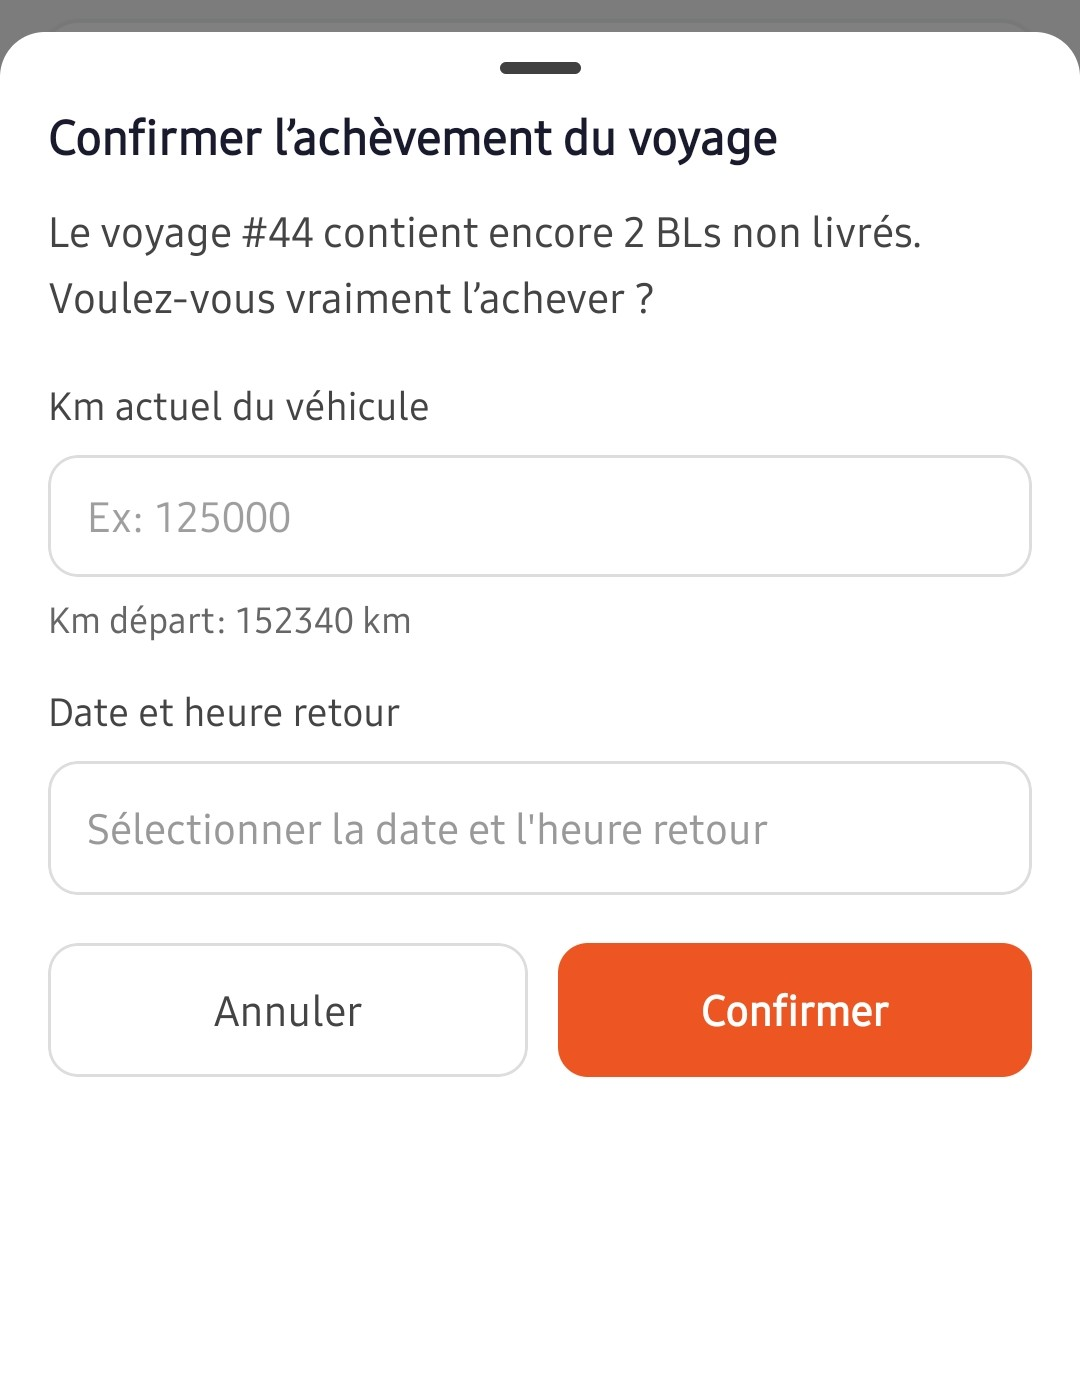
\includegraphics[width=0.9\textwidth]{assets/voyage-achever.jpg}
    }{
    \textit{Achever un voyage : fichier assets/voyage-achever.jpg non trouvé.}
    }
    \caption{Feuille d'achèvement — kilométrage, date et heure retour}
    \label{fig:voyage-achever}
    \end{minipage}\hfill
    \begin{minipage}[b]{0.45\textwidth}
    \centering
    \IfFileExists{assets/voyage-details.jpg}{
    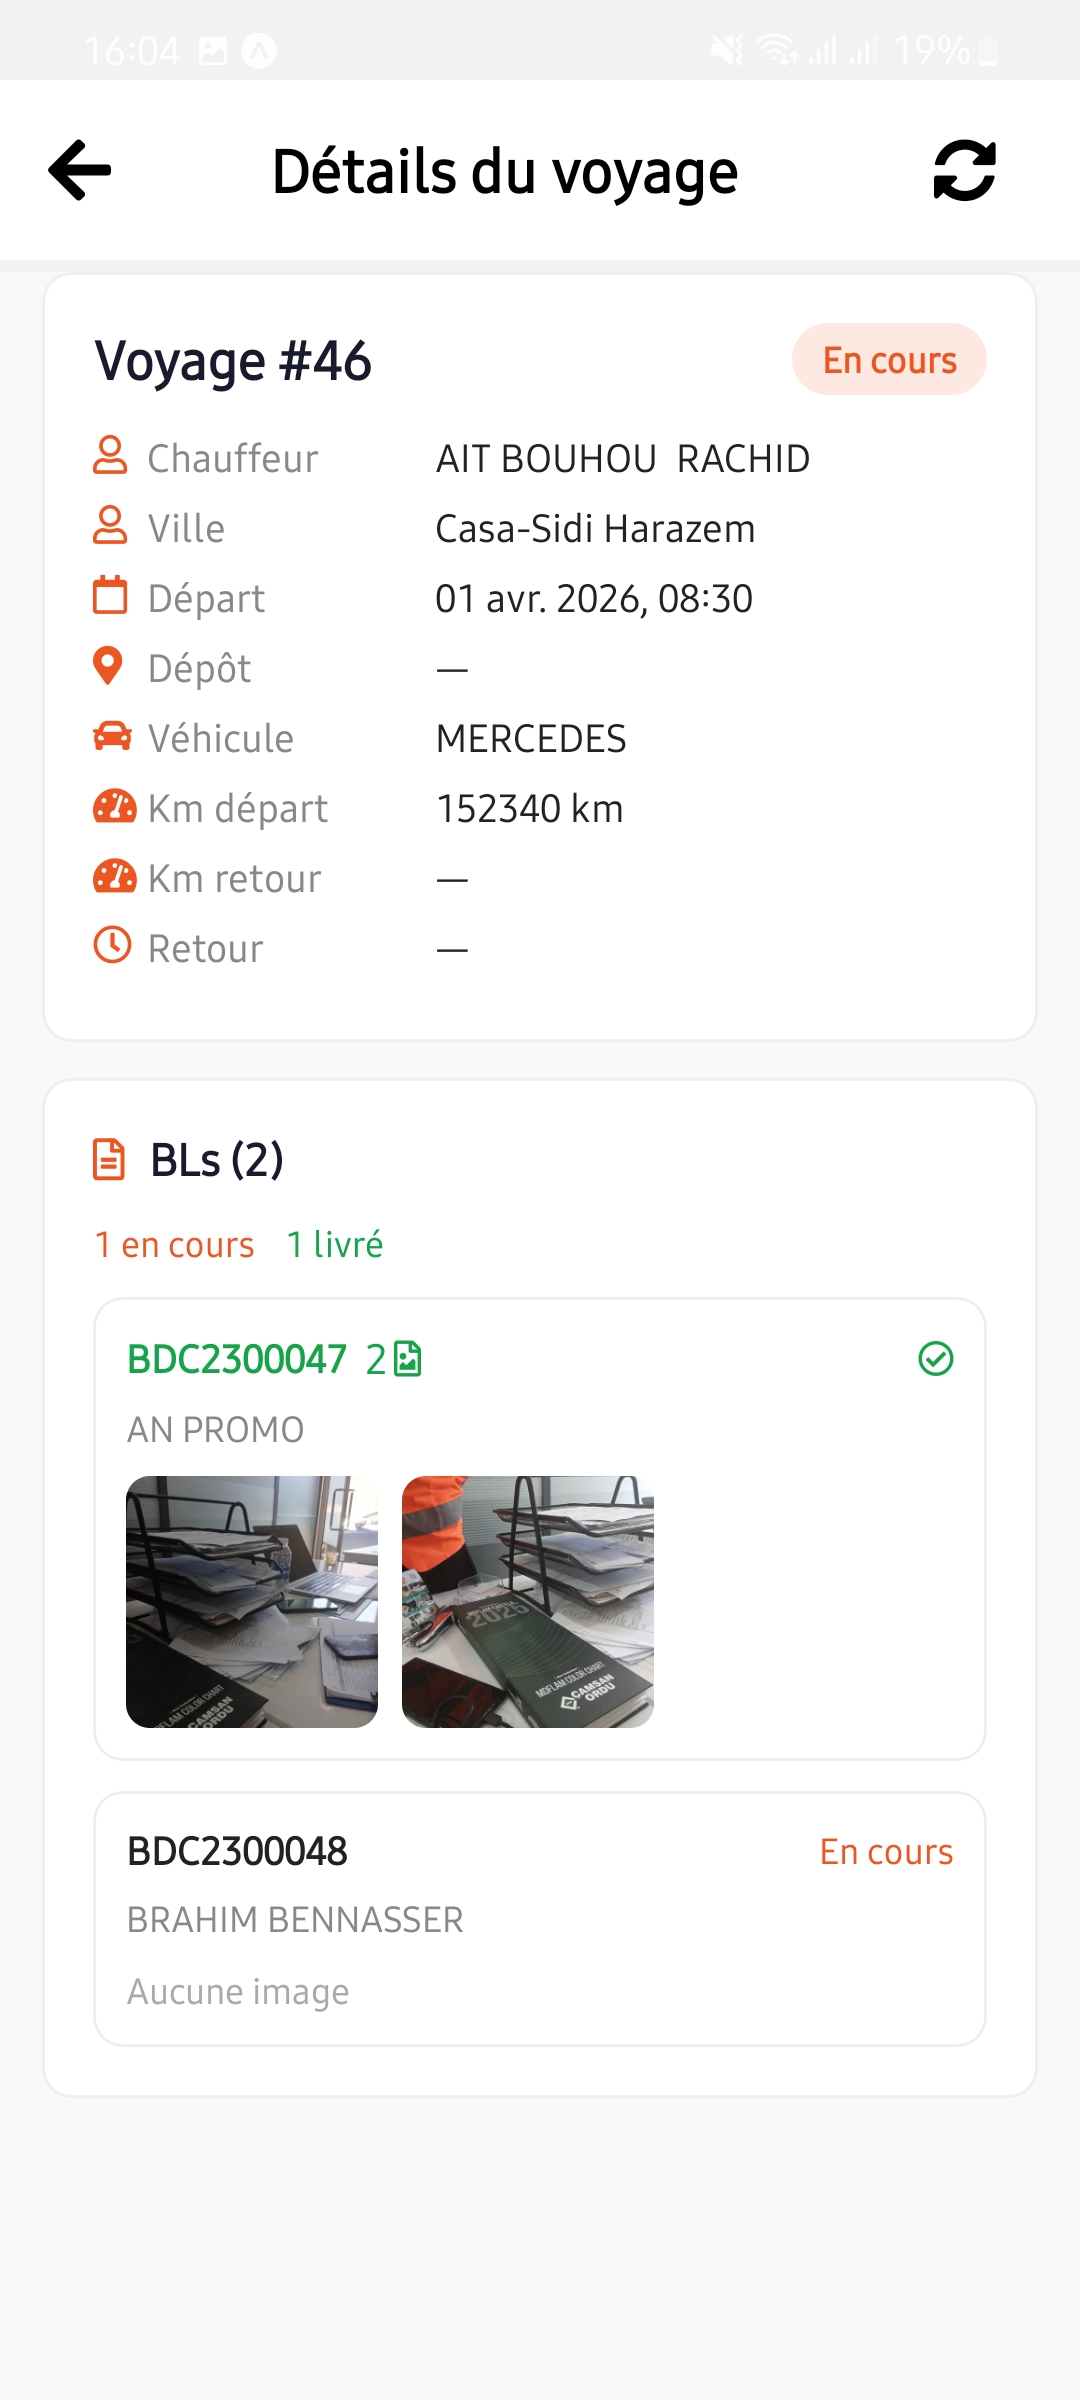
\includegraphics[width=0.9\textwidth]{assets/voyage-details.jpg}
    }{
    \textit{Détail d'un voyage : fichier assets/voyage-details.jpg non trouvé.}
    }
    \caption{Écran de détail — BL, statuts et images}
    \label{fig:voyage-details}
    \end{minipage}
    \end{figure}

    \begin{figure}[H]
    \centering
    \IfFileExists{assets/voyage-delete-confirm.jpg}{
    
\includegraphics[width=0.35\textwidth]{assets/voyage-delete-confirm.jpg}
    }{
    \textit{Confirmation de suppression : fichier assets/voyage-delete-confirm.jpg non trouvé.}
    }
    \caption{Feuille de confirmation de suppression d'un voyage}
    \label{fig:voyage-delete-confirm}
    \end{figure}

    \subsection{Sprint 3 : Module Retours chauffeur et Rapports qualité}

    Le module Retours chauffeur permet aux chauffeurs de soumettre des retours de marchandise et aux administrateurs de les valider ou de les refuser. Chaque retour est rattaché à un client et à un chauffeur, et peut inclure des photos prises en direct depuis l'appareil photo du terminal ou des fichiers joints sélectionnés depuis le stockage. Le cycle de vie d'un retour passe par quatre statuts : \og En cours \fg{} lors de la création, \og Envoyé \fg{} après soumission, puis \og Terminé \fg{} si le retour est accepté ou \og Refusé \fg{} si l'administrateur le rejette.

    L'accès au module est contrôlé par cinq permissions : \texttt{LIST} (consultation de la liste), \texttt{CREATE} (création d'un retour), \texttt{UPDATE} (gestion des retours), \texttt{DELETE} (suppression) et \texttt{ACHEVER\_BL} (validation ou refus d'un retour). Seules les personnes autorisées voient les boutons d'action correspondants.

    \subsubsection{Liste des retours et filtrage}

    L'écran principal affiche la liste paginée des retours sous forme de cartes. Chaque carte présente l'identifiant du retour, le nom du chauffeur, le statut coloré et le nombre de fichiers joints. En appuyant sur une carte, des détails supplémentaires apparaissent (client, motif de réclamation, retour MSE, BL cacheté, règlement) ainsi que deux boutons d'action : \og Voir les détails \fg{} et \og Plus \fg{} (traitement ou suppression).

    Une barre de recherche locale permet de filtrer la liste. Un bouton de filtre ouvre une feuille modale proposant deux critères serveur : le chauffeur et le client (avec recherche intégrée). Un badge indique le nombre de filtres actifs.

    La Figure~\ref{fig:retour-list} présente la liste des retours avec la barre de recherche et le bouton de création.

    \begin{figure}[ht]
    \centering
    \IfFileExists{assets/retour-list.jpg}{
    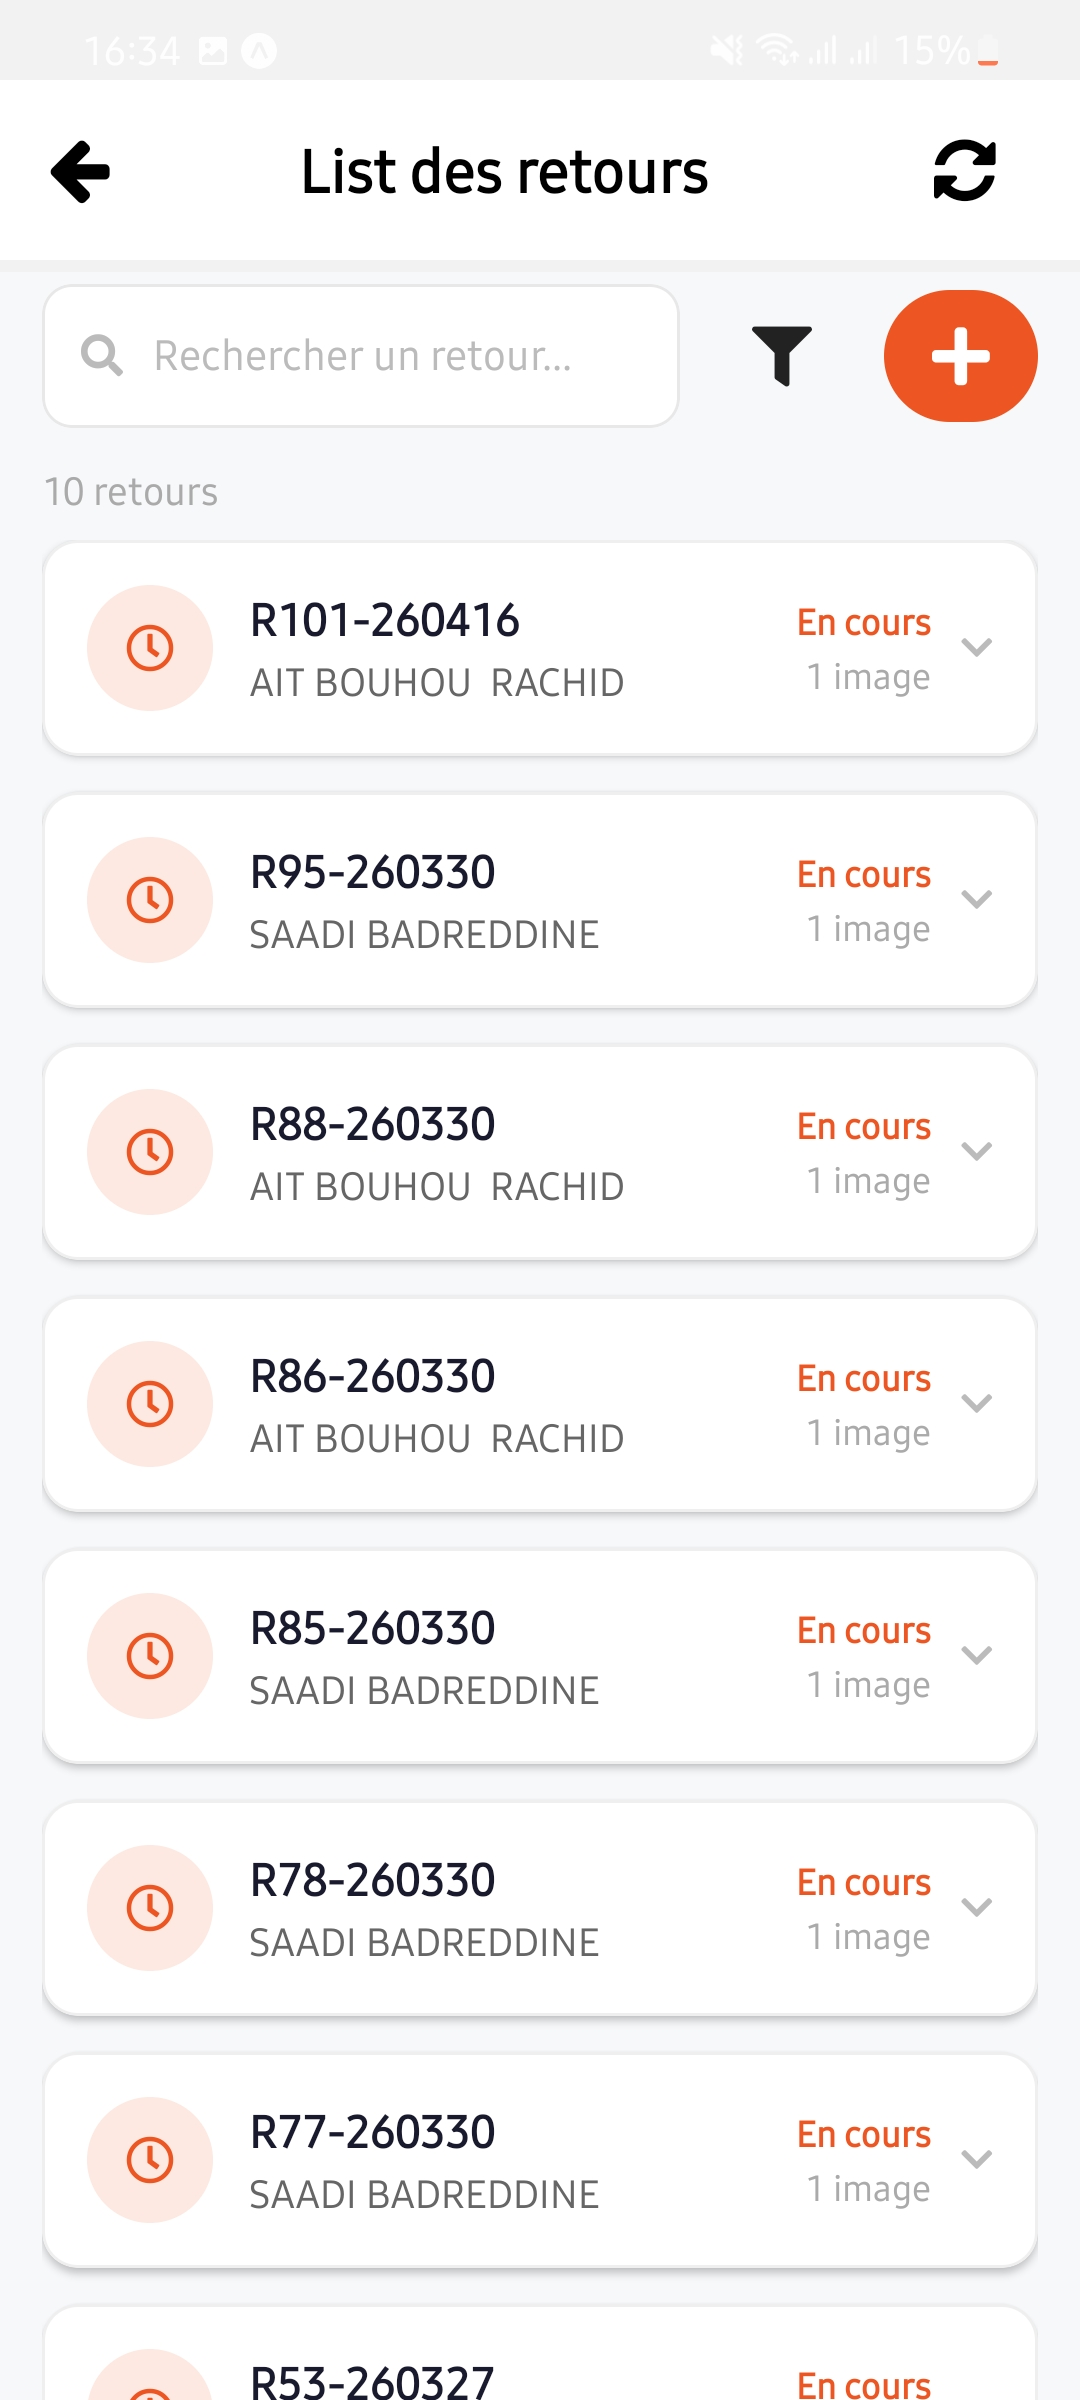
\includegraphics[width=0.35\textwidth]{assets/retour-list.jpg}
    }{
    \textit{Liste des retours : fichier assets/retour-list.jpg non trouvé.}
    }
    \caption{Liste des retours — cartes avec identifiant, chauffeur et statut}
    \label{fig:retour-list}
    \end{figure}

    \subsubsection{Carte expansive, filtrage et détail}

    La carte expansive dévoile les détails du retour (client, motif de réclamation, indicateurs booléens) et propose les boutons Voir les détails et Plus (traitement, suppression). L'écran de détail affiche toutes les informations du retour, le commentaire éventuel de validation dans un encadré coloré, ainsi que la liste des fichiers joints avec les actions Aperçu, Télécharger et Partager. L'écran de filtrage permet de filtrer la liste par chauffeur et par client.

    La Figure~\ref{fig:retour-filter} illustre la feuille de filtrage, la Figure~\ref{fig:retour-card-expanded} présente la carte expansive, et la Figure~\ref{fig:retour-details} montre l'écran de détail.

    \begin{figure}[ht]
    \centering
    \begin{minipage}[b]{0.32\textwidth}
    \centering
    \IfFileExists{assets/retour-filter.jpg}{
    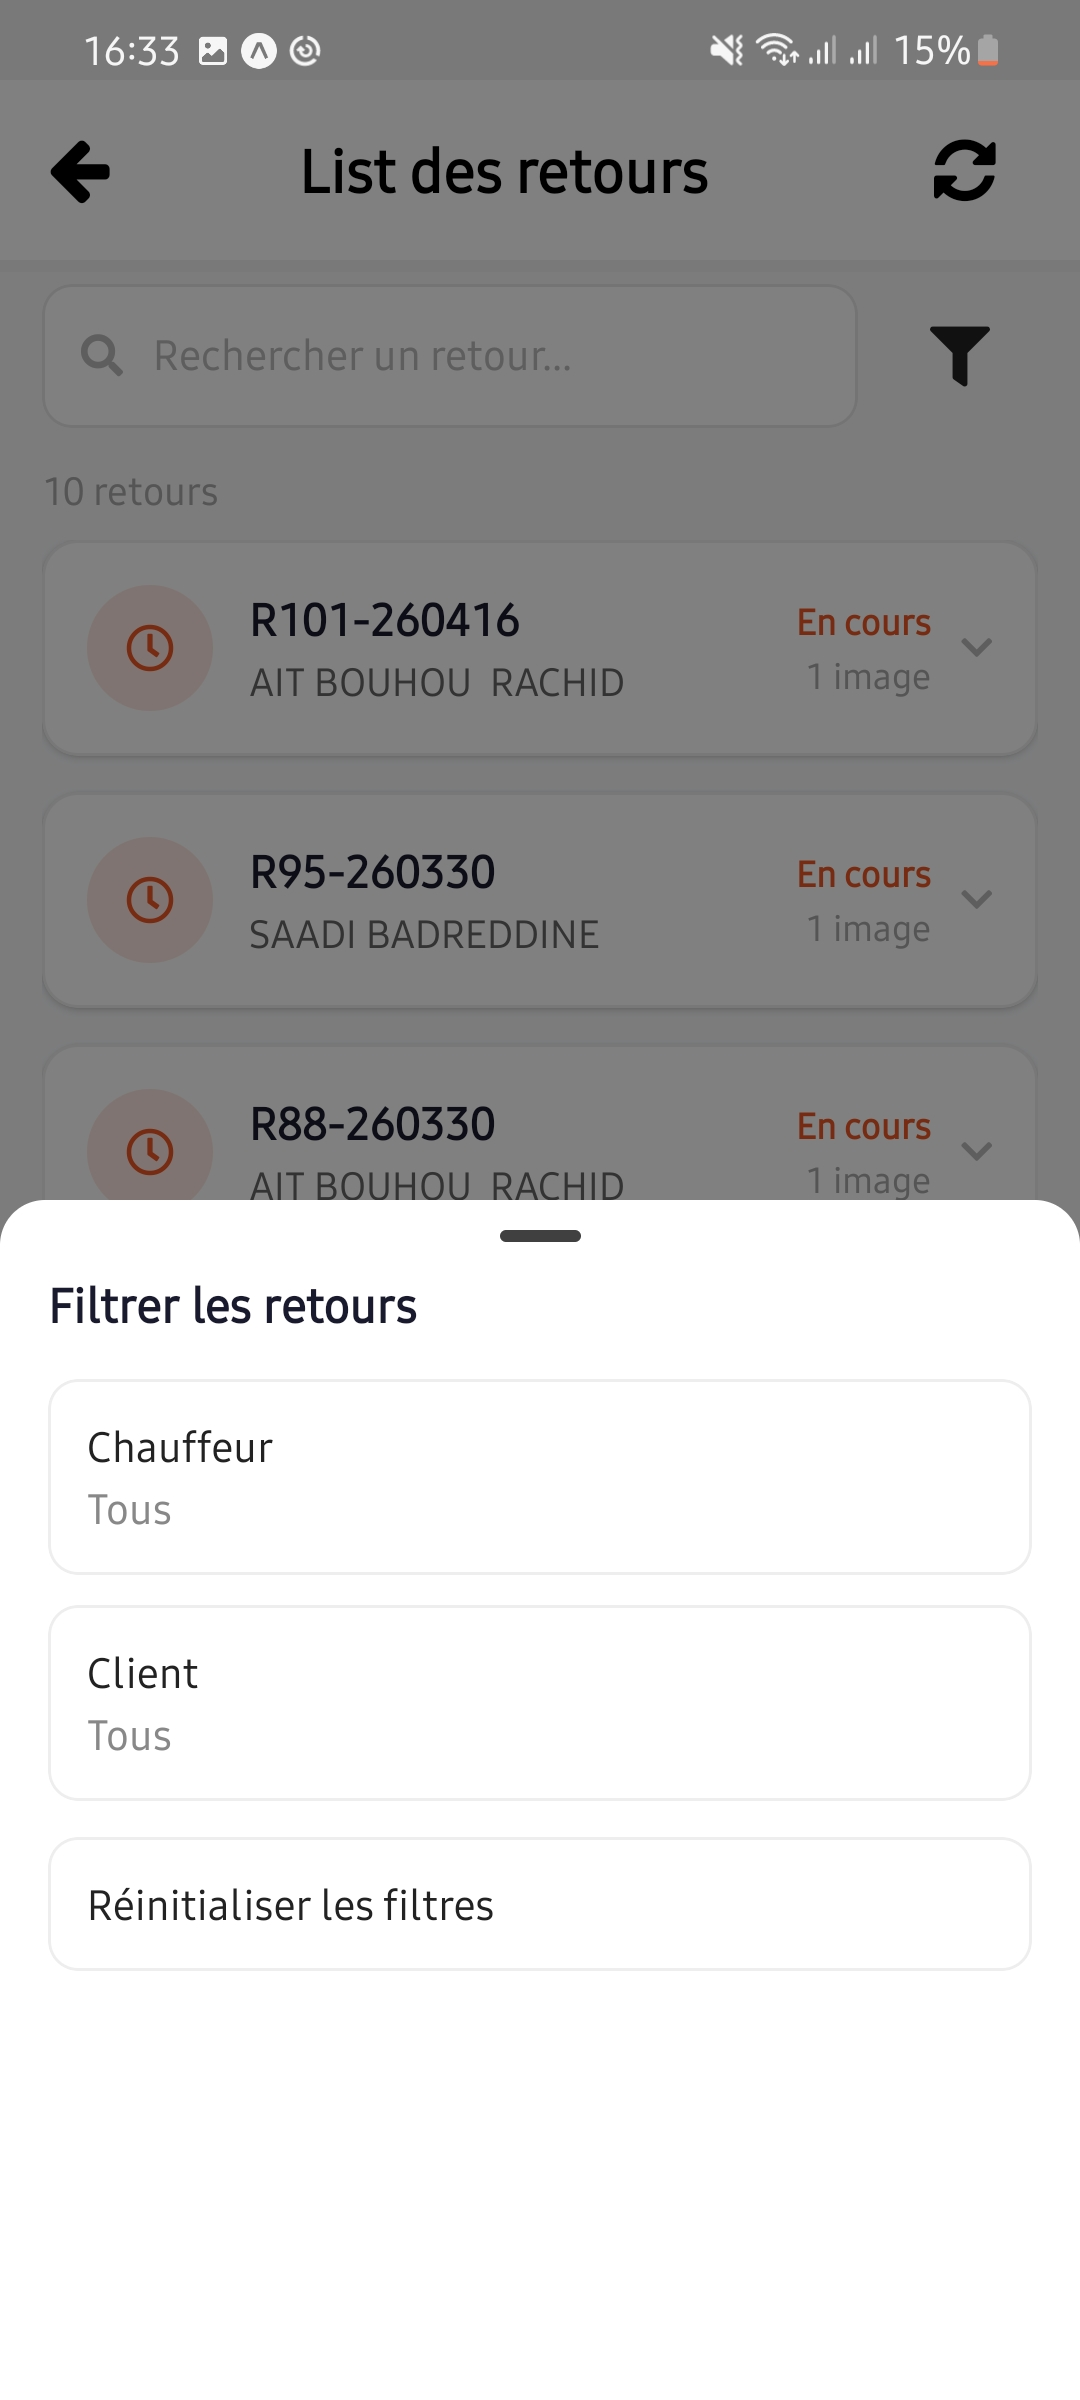
\includegraphics[width=\textwidth]{assets/retour-filter.jpg}
    }{
    \textit{Filtre : fichier assets/retour-filter.jpg non trouvé.}
    }
    \caption{Feuille de filtrage par chauffeur et client}
    \label{fig:retour-filter}
    \end{minipage}\hfill
    \begin{minipage}[b]{0.32\textwidth}
    \centering
    \IfFileExists{assets/retour-card-expanded.jpg}{
    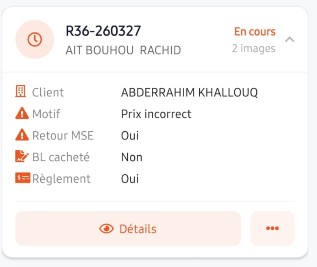
\includegraphics[width=\textwidth]{assets/retour-card-expanded.jpg}
    }{
    \textit{Carte expansive : fichier assets/retour-card-expanded.jpg non trouvé.}
    }
    \caption{Carte de retour expansée — détails et actions}
    \label{fig:retour-card-expanded}
    \end{minipage}\hfill
    \begin{minipage}[b]{0.32\textwidth}
    \centering
    \IfFileExists{assets/retour-details.jpg}{
    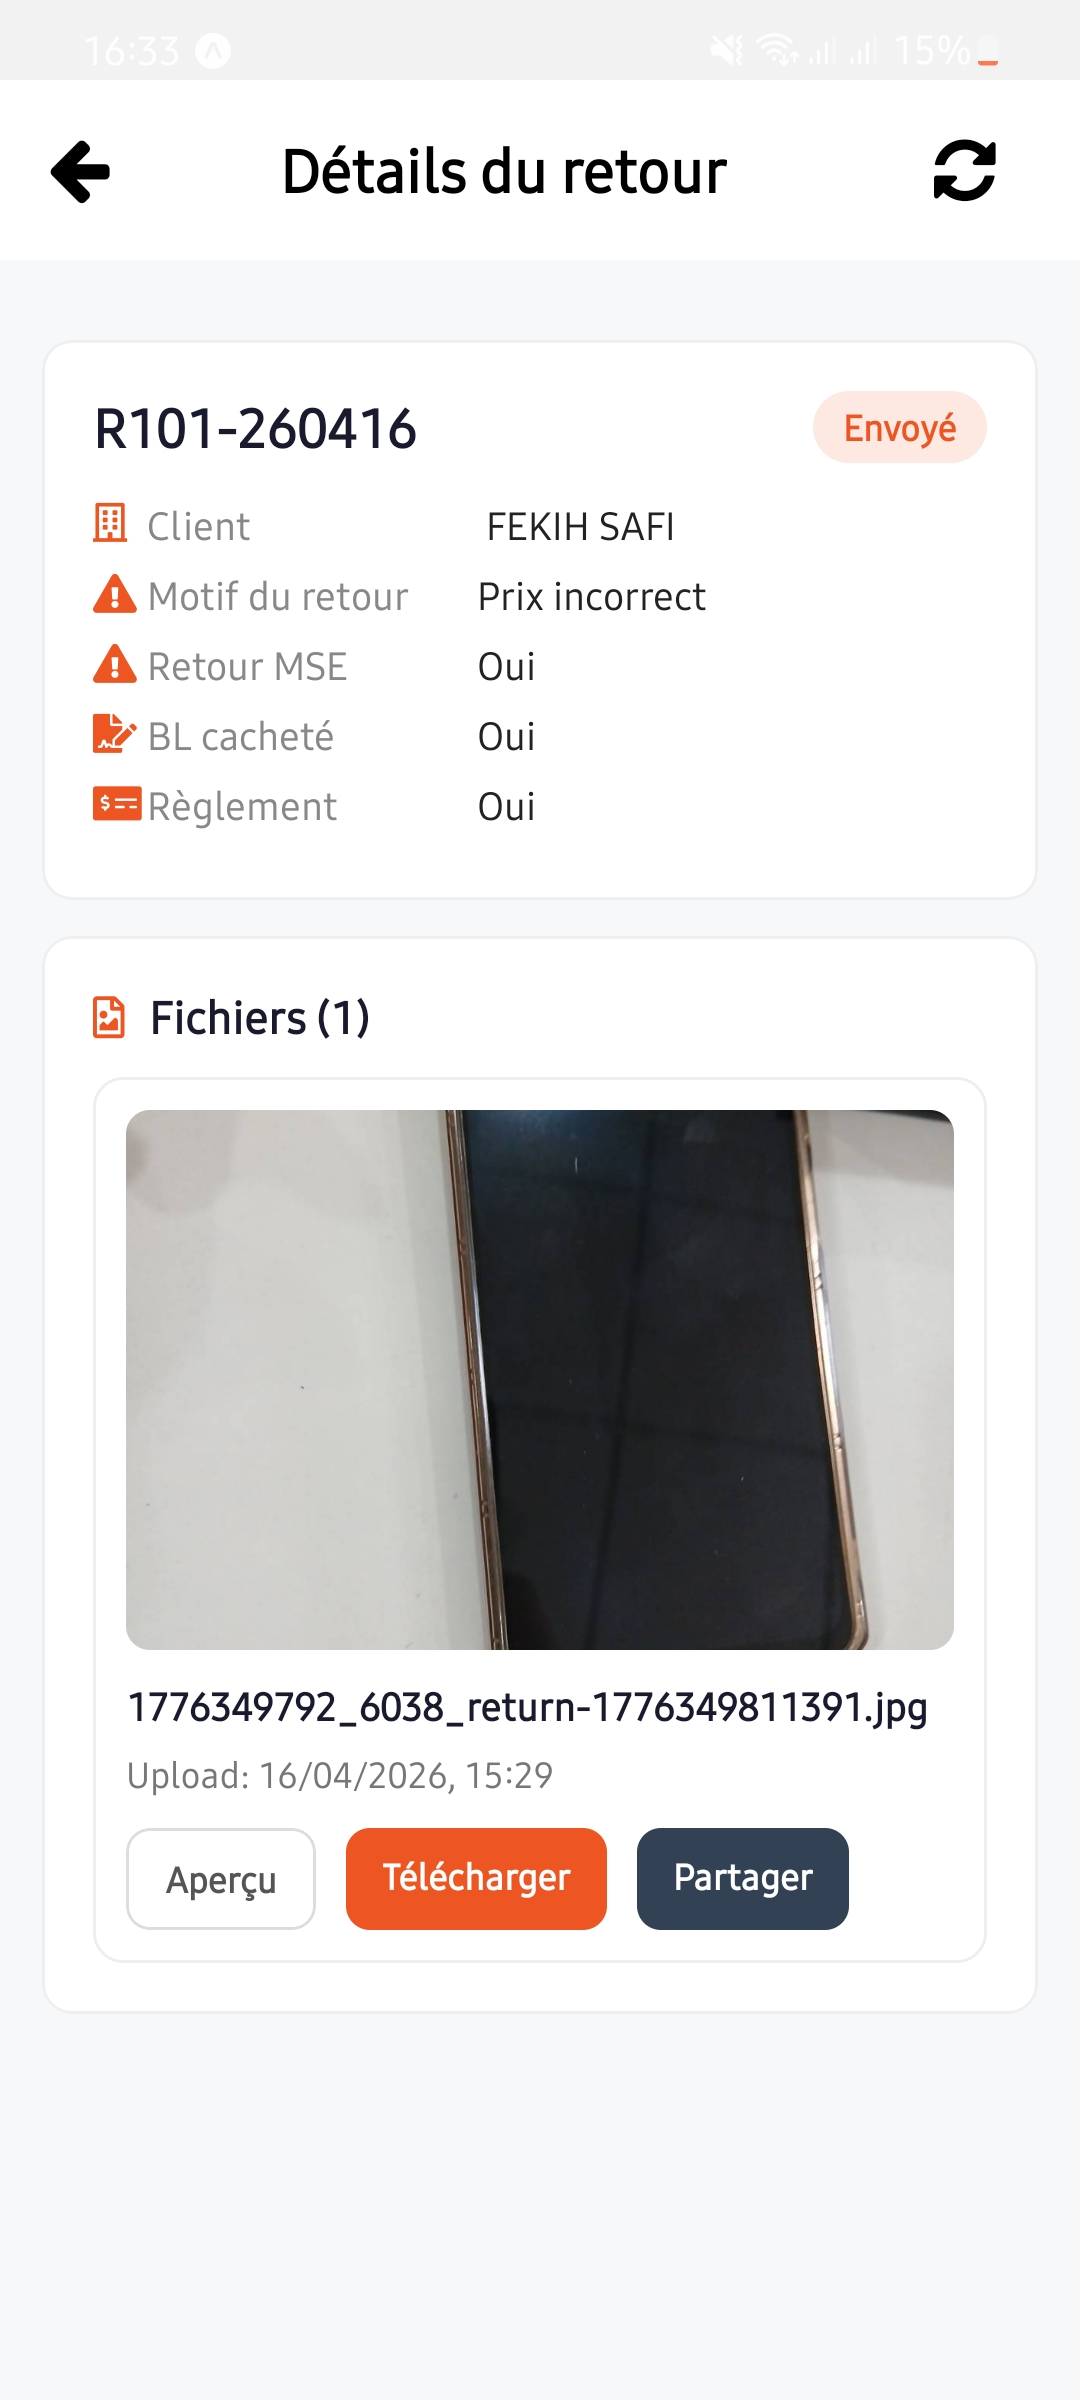
\includegraphics[width=\textwidth]{assets/retour-details.jpg}
    }{
    \textit{Écran de détail : fichier assets/retour-details.jpg non trouvé.}
    }
    \caption{Écran de détail — informations et fichiers joints}
    \label{fig:retour-details}
    \end{minipage}
    \end{figure}

    \subsubsection{Validation, création et suppression}

    La validation d'un retour s'effectue en deux étapes : l'administrateur choisit entre Accepter et Refuser, saisit un commentaire facultatif, puis confirme son choix sur un écran récapitulatif avec un bouton coloré selon l'action (vert pour acceptation, rouge pour refus).

    La création d'un retour comporte un formulaire (client, BL cacheté, règlement, retour MSE, réclamation) et une zone de fichiers permettant de prendre une photo via l'appareil photo du terminal ou de sélectionner des fichiers depuis le stockage, avec un aperçu en liste horizontale.

    La suppression affiche une feuille de confirmation avec le message \og Le retour \#\{id\} sera supprimé définitivement. Voulez-vous continuer ? \fg{} et deux boutons : Annuler ou Supprimer.

    La Figure~\ref{fig:retour-validation} présente l'écran de validation, la Figure~\ref{fig:retour-create} montre l'écran de création, et la Figure~\ref{fig:retour-delete-confirm} illustre la confirmation de suppression.

    \begin{figure}[ht]
    \centering
    \begin{minipage}[b]{0.32\textwidth}
    \centering
    \IfFileExists{assets/retour-validation.jpg}{
    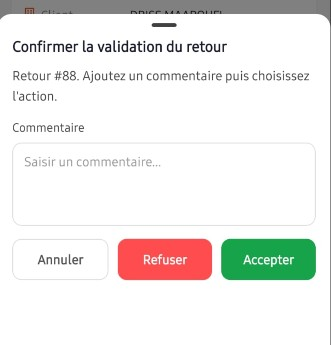
\includegraphics[width=\textwidth]{assets/retour-validation.jpg}
    }{
    \textit{Validation : fichier assets/retour-validation.jpg non trouvé.}
    }
    \caption{Validation — Choix, commentaire et confirmation}
    \label{fig:retour-validation}
    \end{minipage}\hfill
    \begin{minipage}[b]{0.32\textwidth}
    \centering
    \IfFileExists{assets/retour-create.jpg}{
    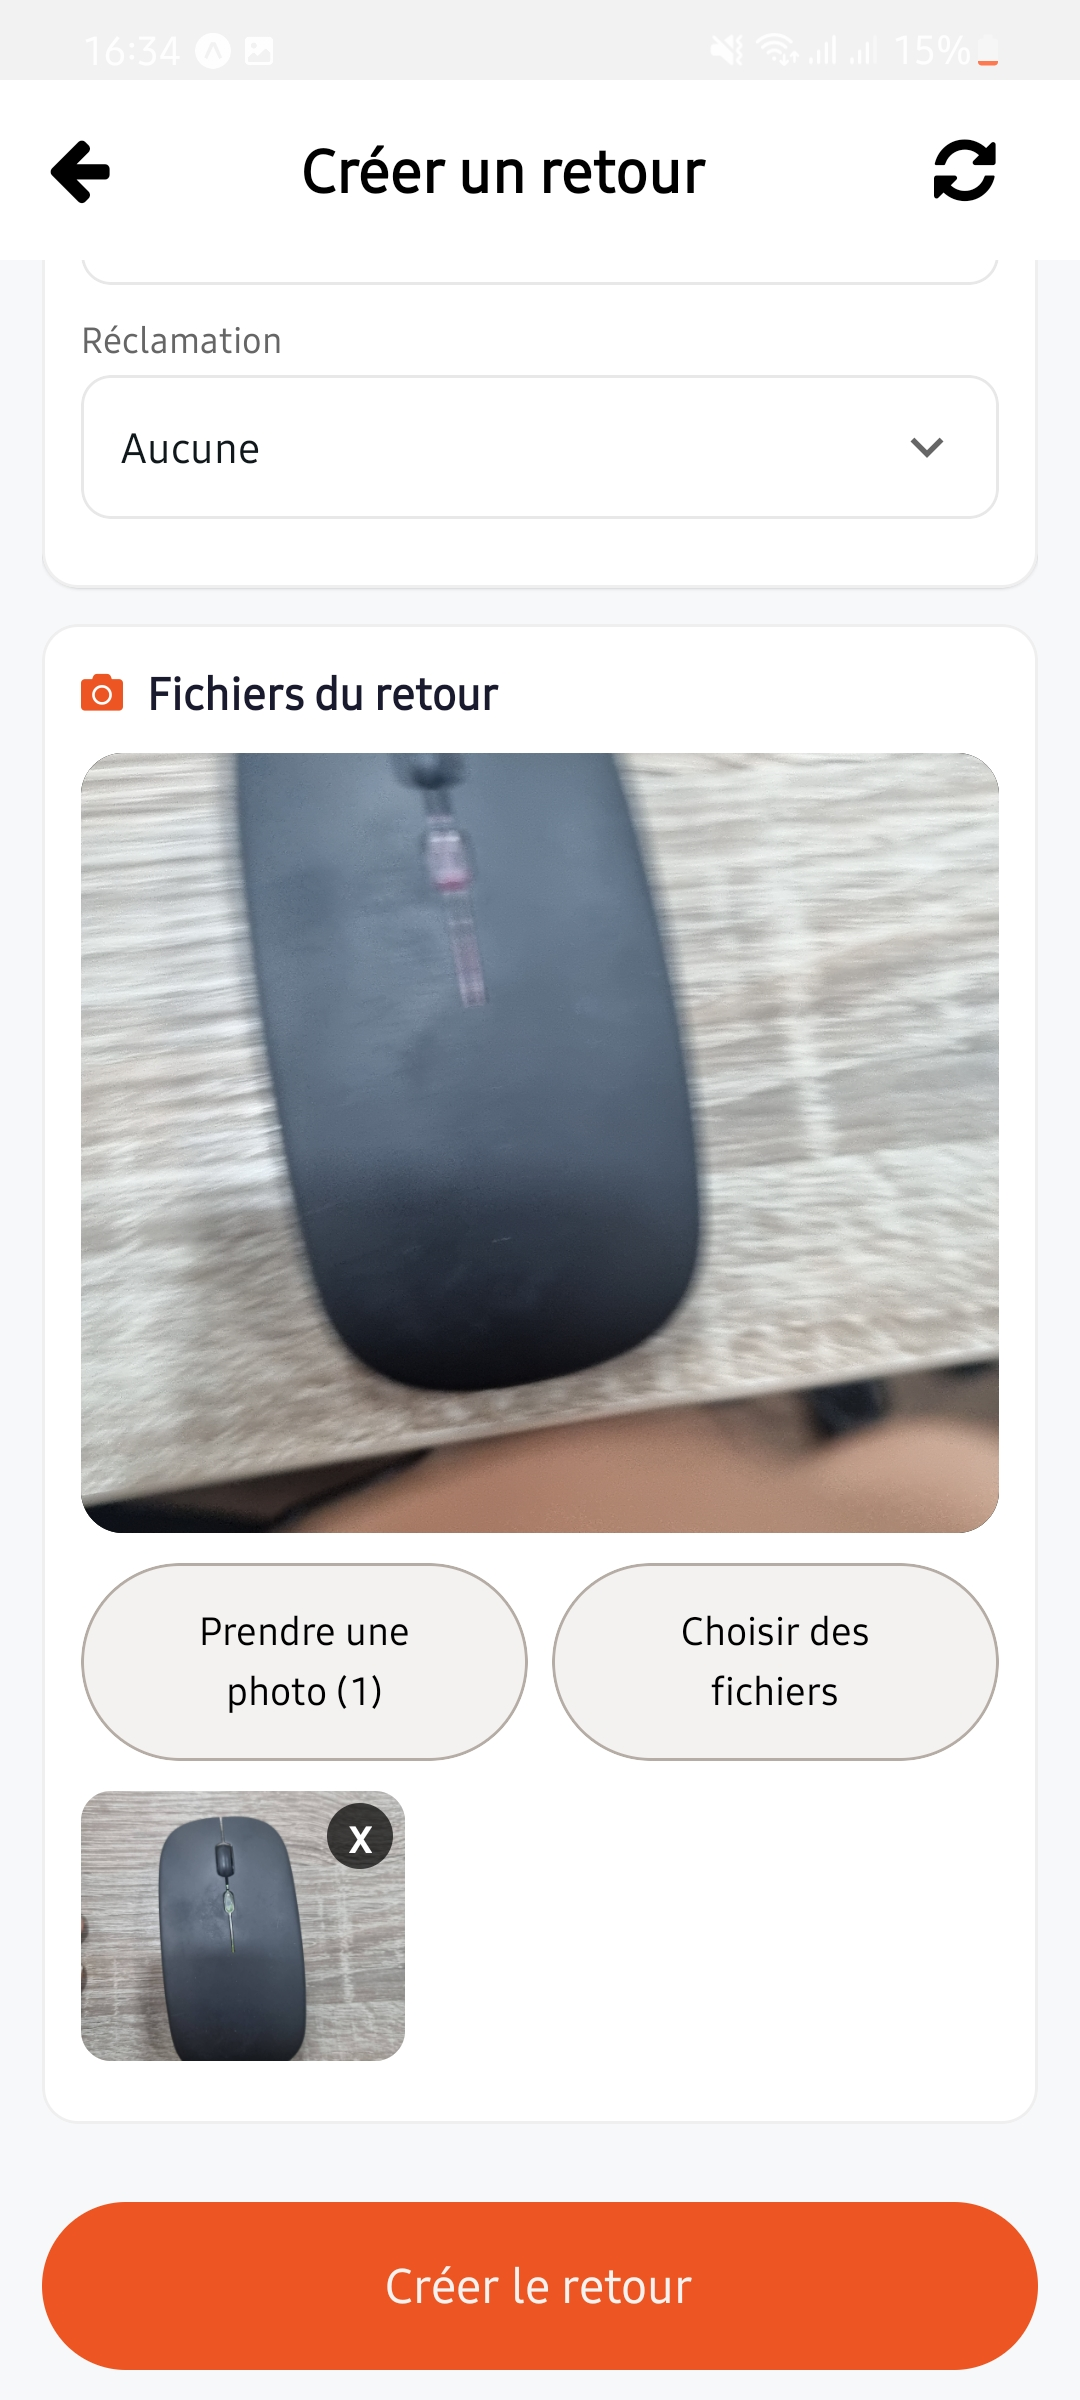
\includegraphics[width=\textwidth]{assets/retour-create.jpg}
    }{
    \textit{Création : fichier assets/retour-create.jpg non trouvé.}
    }
    \caption{Création d'un retour — formulaire et prise de photos}
    \label{fig:retour-create}
    \end{minipage}\hfill
    \begin{minipage}[b]{0.32\textwidth}
    \centering
    \IfFileExists{assets/retour-delete-confirm.jpg}{
    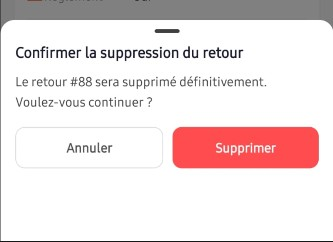
\includegraphics[width=\textwidth]{assets/retour-delete-confirm.jpg}
    }{
    \textit{Suppression : fichier assets/retour-delete-confirm.jpg non trouvé.}
    }
    \caption{Feuille de confirmation de suppression d'un retour}
    \label{fig:retour-delete-confirm}
    \end{minipage}
    \end{figure}

    \subsubsection{Module Rapports qualité}

    Le module Rapports qualité permet de consigner des rapports sur la qualité des produits livrés. Chaque rapport est identifié par un numéro, contient les champs DUM, Dossier et Commentaire, et peut être accompagné de fichiers joints (photos ou documents). L'accès est contrôlé par quatre permissions : \texttt{LIST} (consultation), \texttt{CREATE} (création), \texttt{UPDATE} (modification) et \texttt{DELETE} (suppression).

    \subsubsection{Liste des rapports et carte expansive}

    L'écran principal affiche la liste paginée des rapports sous forme de cartes. Chaque carte présente l'identifiant du rapport (\texttt{RQ-\{id\}}), le dossier ou DUM, la date de création et le nombre de fichiers joints. En appuyant sur une carte, des détails supplémentaires apparaissent : les champs DUM, Dossier, Commentaire et Date, accompagnés d'une galerie de miniatures des fichiers joints et de deux boutons d'action conditionnels — \og Détails \fg{} et \og Supprimer \fg.

    Une barre de recherche locale avec débounce permet de filtrer les rapports par DUM, Dossier ou Commentaire.

    La Figure~\ref{fig:rapport-qualite-list} présente la liste des rapports, et les Figures~\ref{fig:rapport-qualite-card-expanded} et~\ref{fig:rapport-qualite-details} illustrent respectivement la carte expansive et l'écran de détail.

    \begin{figure}[ht]
    \centering
    \IfFileExists{assets/rapport-qualite-list.jpg}{
    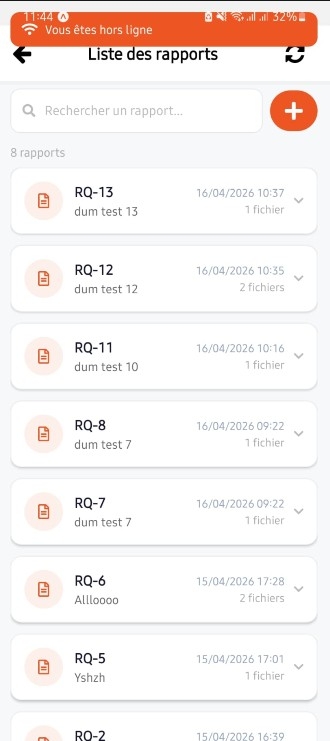
\includegraphics[width=0.35\textwidth]{assets/rapport-qualite-list.jpg}
    }{
    \textit{Liste des rapports : fichier assets/rapport-qualite-list.jpg non trouvé.}
    }
    \caption{Liste des rapports qualité — cartes avec DUM et Dossier}
    \label{fig:rapport-qualite-list}
    \end{figure}

    \begin{figure}[ht]
    \centering
    \begin{minipage}[b]{0.45\textwidth}
    \centering
    \IfFileExists{assets/rapport-qualite-card-expanded.jpg}{
    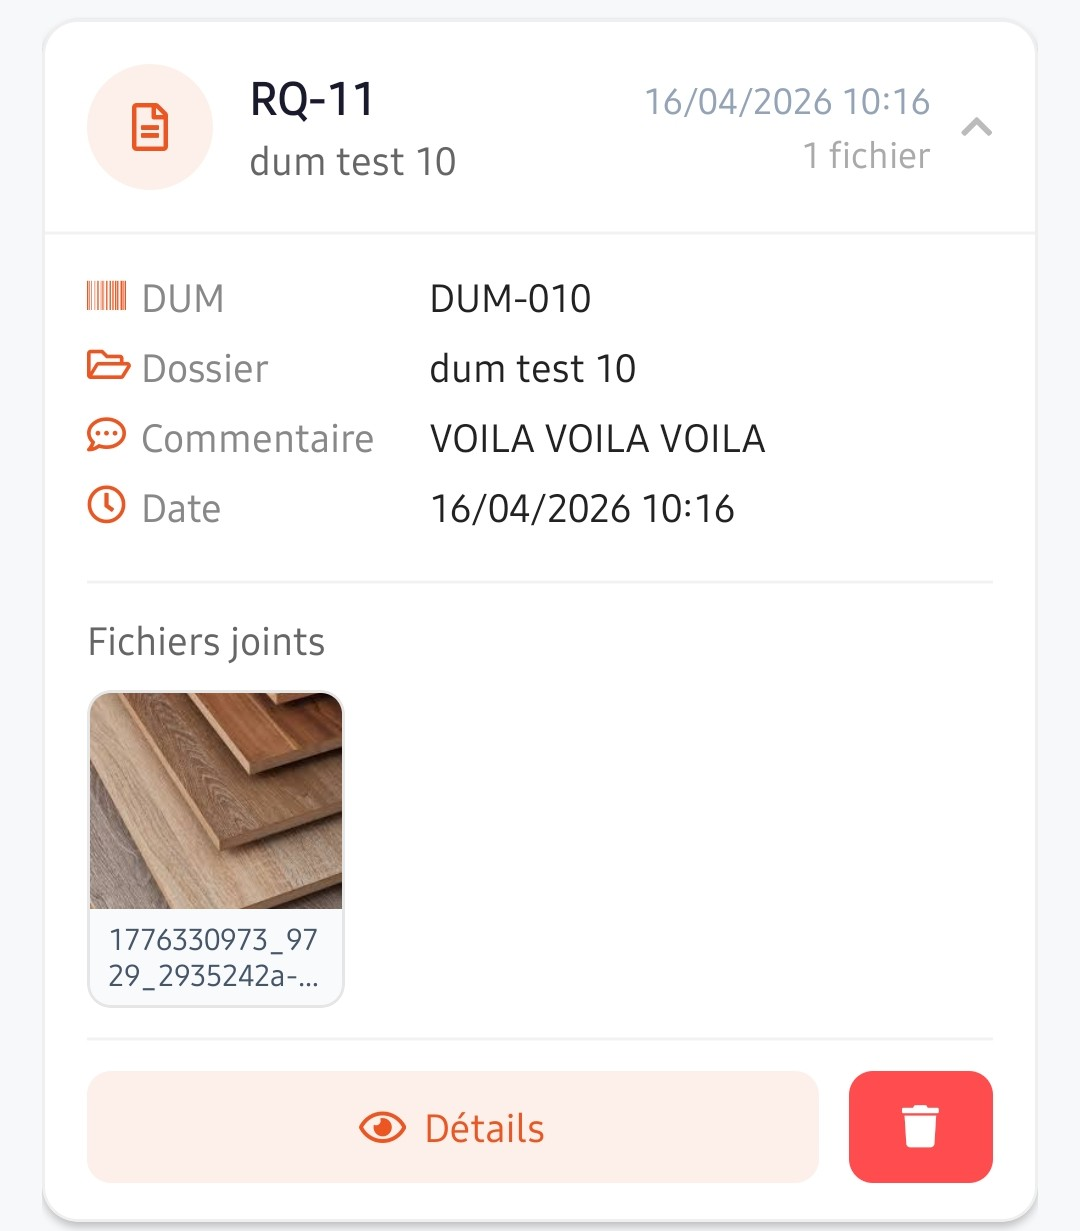
\includegraphics[width=0.85\textwidth]{assets/rapport-qualite-card-expanded.jpg}
    }{
    \textit{Carte expansive : fichier assets/rapport-qualite-card-expanded.jpg non trouvé.}
    }
    \caption{Carte de rapport expansive — détails et actions}
    \label{fig:rapport-qualite-card-expanded}
    \end{minipage}\hfill
    \begin{minipage}[b]{0.45\textwidth}
    \centering
    \IfFileExists{assets/rapport-qualite-details.jpg}{
    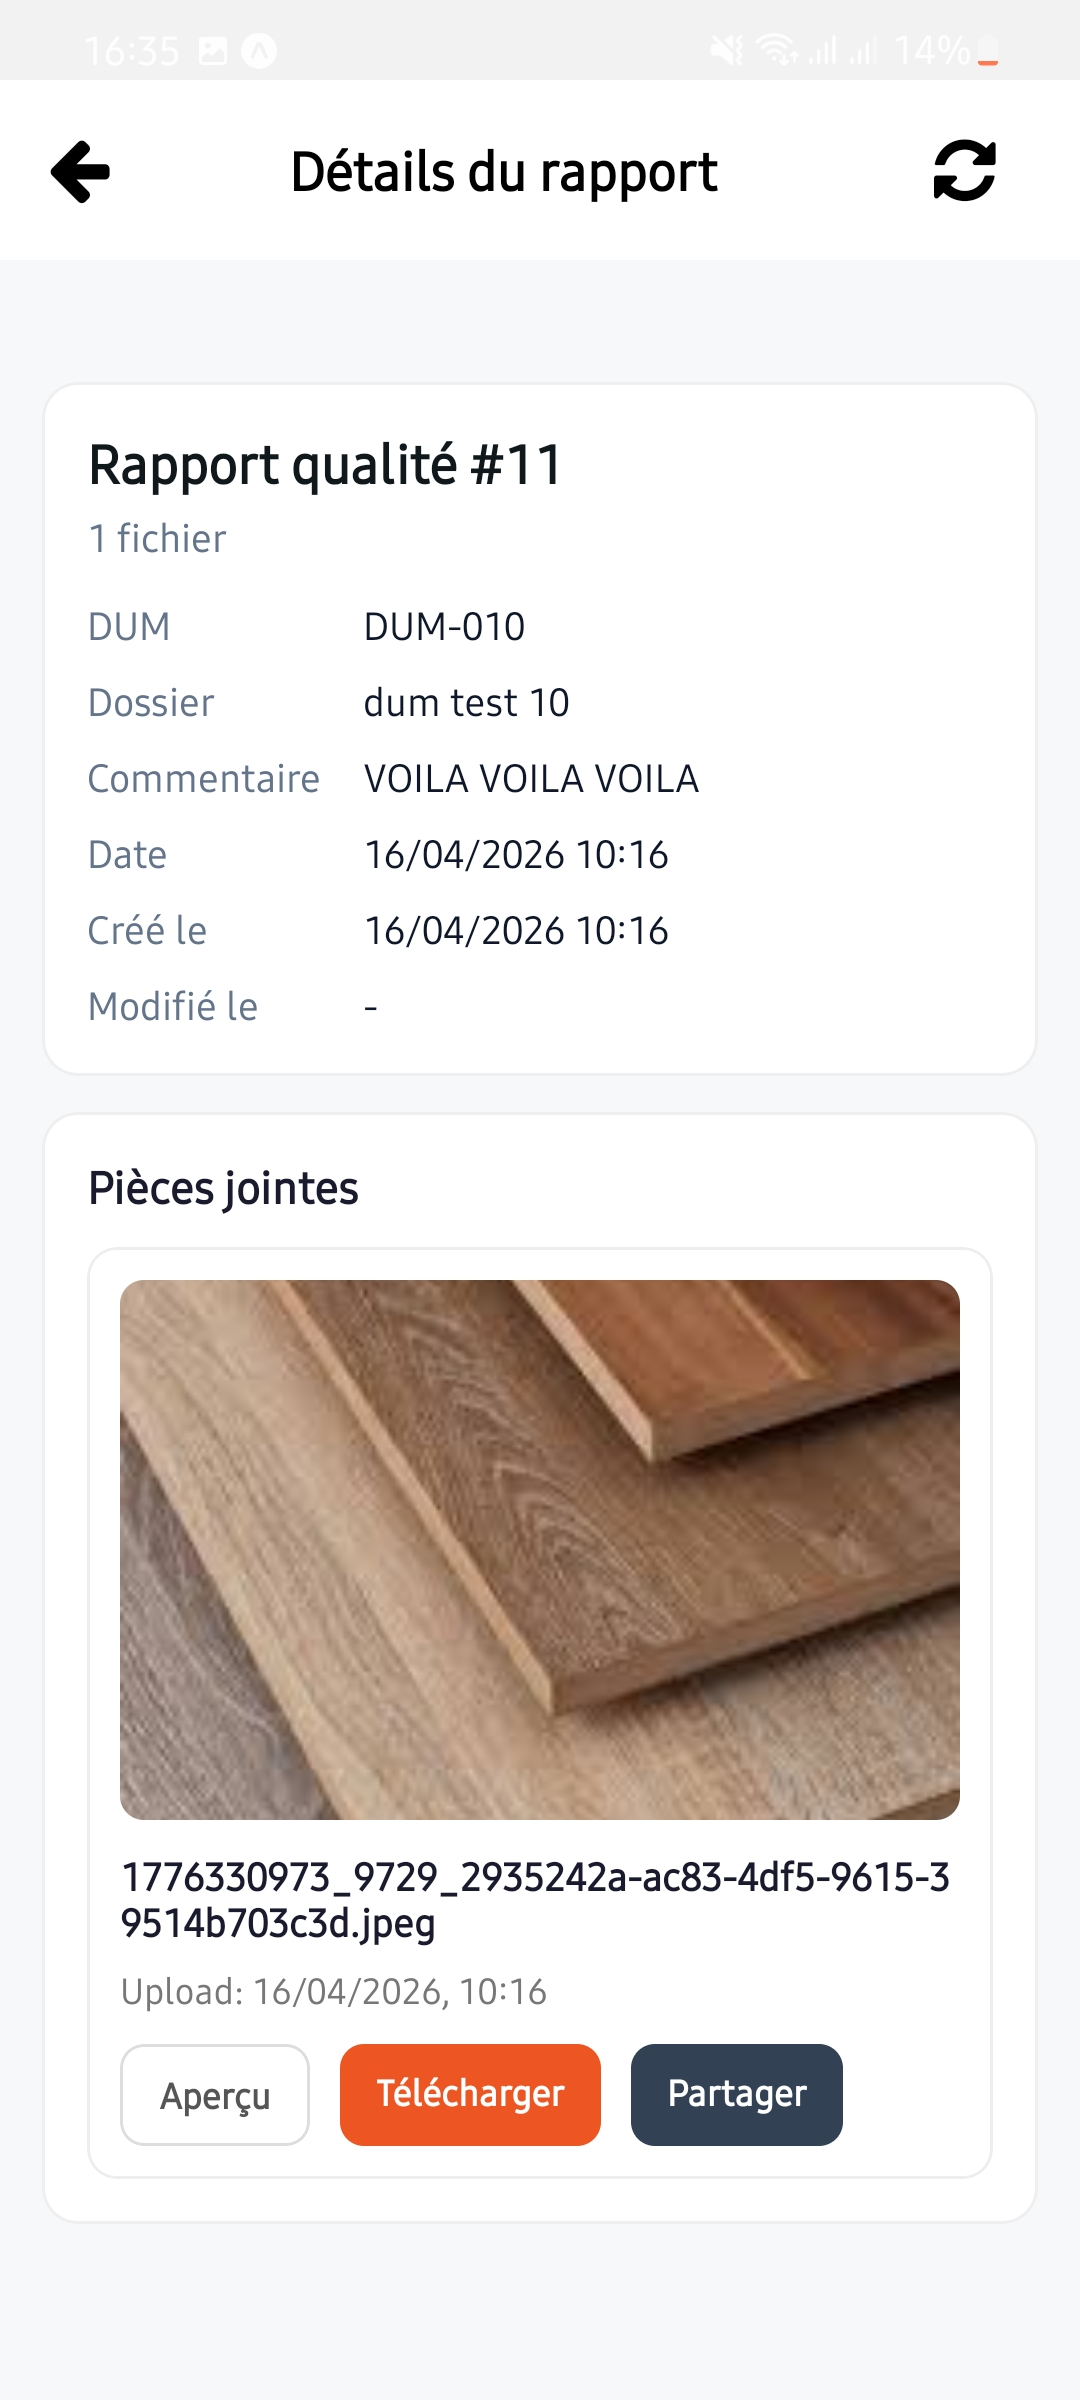
\includegraphics[width=0.85\textwidth]{assets/rapport-qualite-details.jpg}
    }{
    \textit{Écran de détail : fichier assets/rapport-qualite-details.jpg non trouvé.}
    }
    \caption{Écran de détail — informations et fichiers joints}
    \label{fig:rapport-qualite-details}
    \end{minipage}
    \end{figure}

    \subsubsection{Création et suppression}

    L'écran de création comporte un formulaire (DUM, Dossier, Commentaire) et une zone de fichiers permettant de prendre une photo depuis l'appareil photo ou de sélectionner des fichiers existants, avec un aperçu en liste horizontale. La validation exige qu'au moins un des champs DUM ou Dossier soit renseigné et qu'au moins un fichier soit joint.

    La suppression affiche une feuille de confirmation avec le message \og Le rapport \#\{id\} sera supprimé définitivement. Voulez-vous continuer ? \fg{} et deux boutons : Annuler ou Supprimer.

    La Figure~\ref{fig:rapport-qualite-create} présente l'écran de création, et la Figure~\ref{fig:rapport-qualite-delete-confirm} illustre la confirmation de suppression.

    \begin{figure}[ht]
    \centering
    \begin{minipage}[b]{0.45\textwidth}
    \centering
    \IfFileExists{assets/rapport-qualite-create.jpg}{
    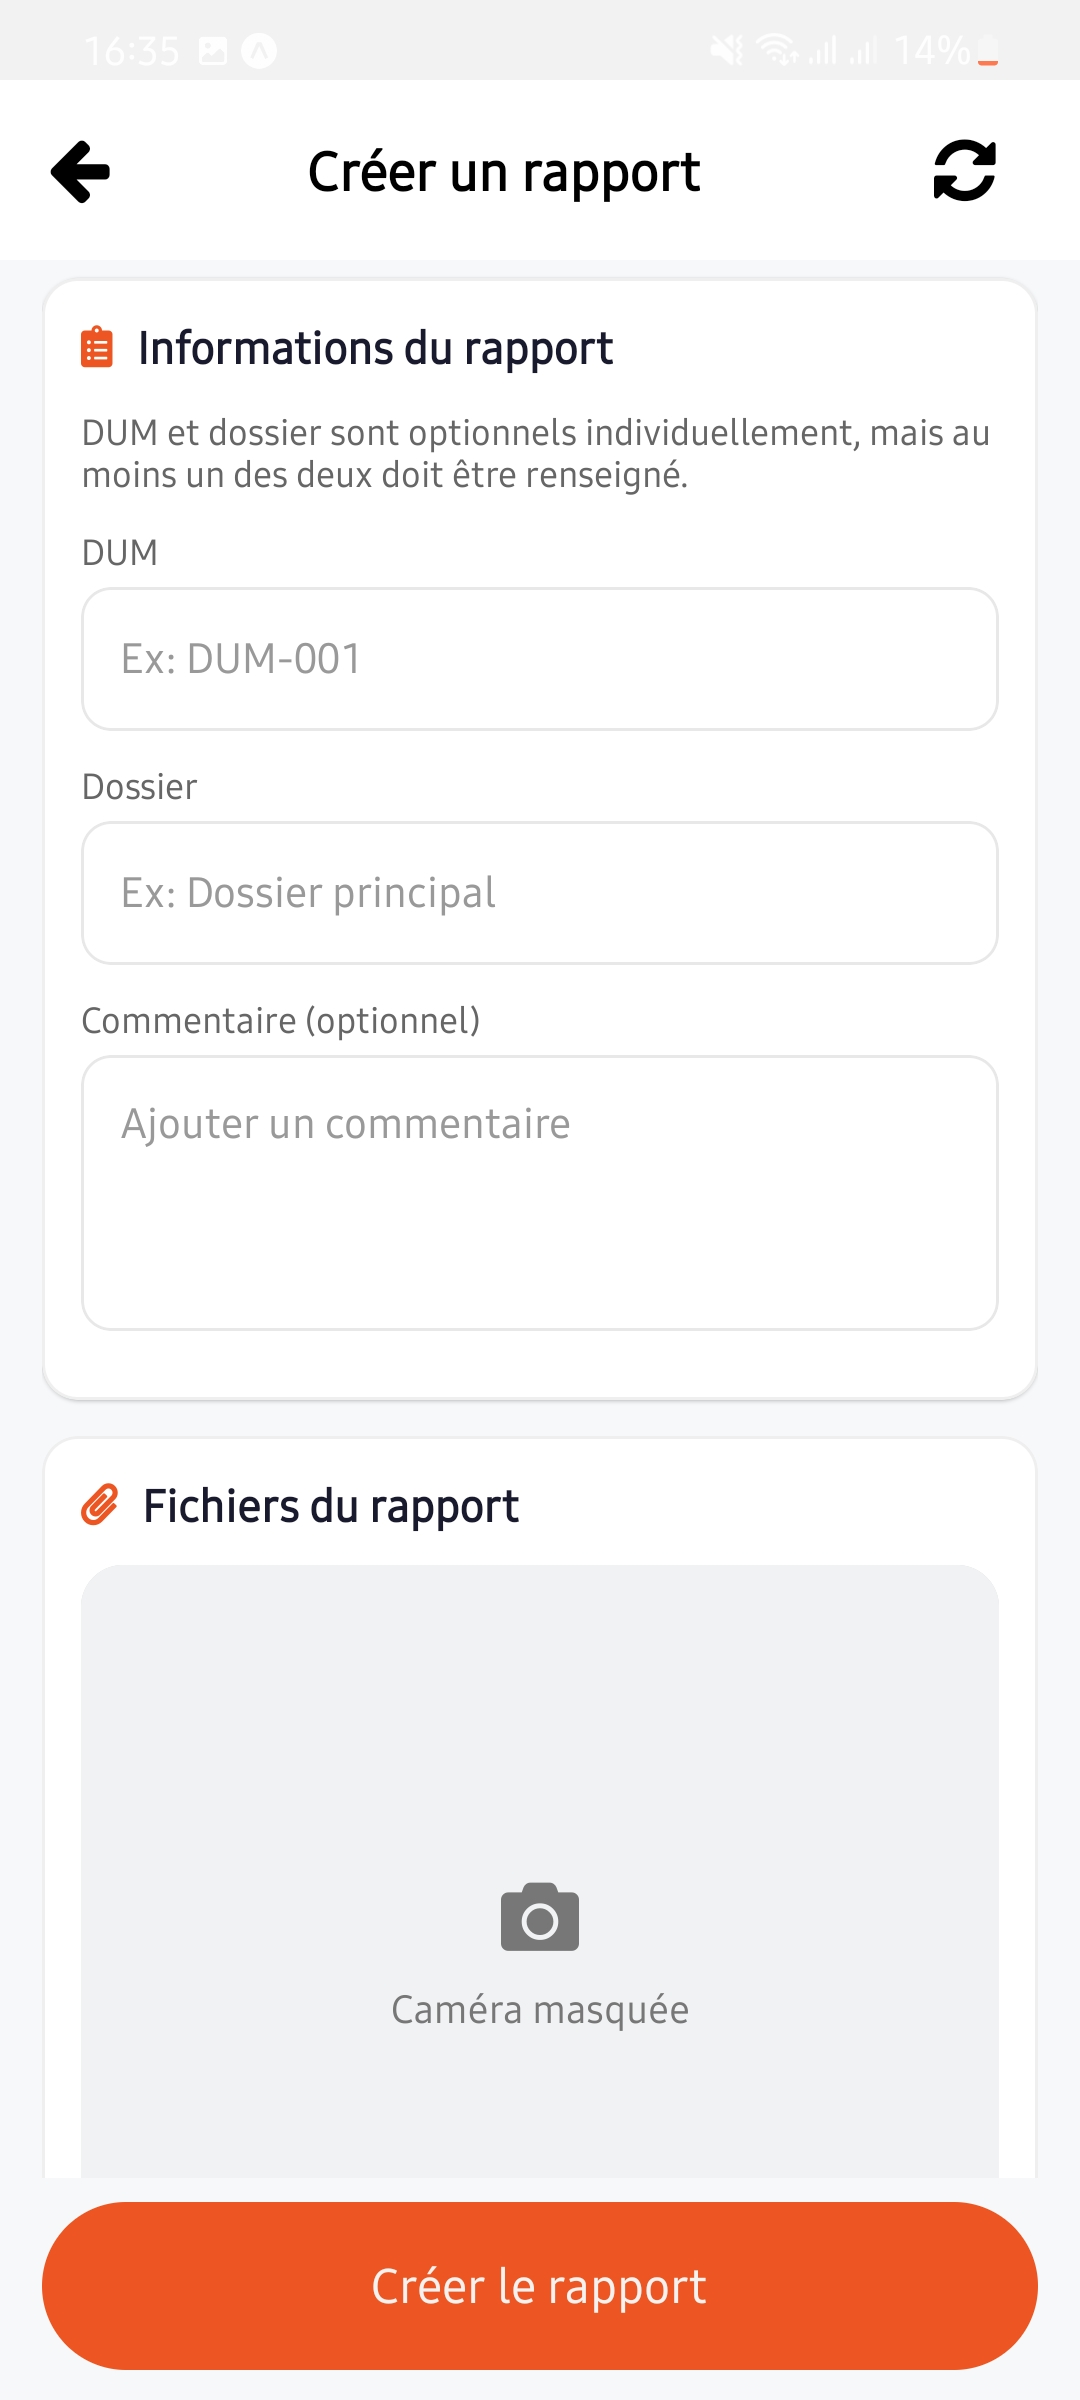
\includegraphics[width=0.85\textwidth]{assets/rapport-qualite-create.jpg}
    }{
    \textit{Création : fichier assets/rapport-qualite-create.jpg non trouvé.}
    }
    \caption{Création d'un rapport qualité}
    \label{fig:rapport-qualite-create}
    \end{minipage}\hfill
    \begin{minipage}[b]{0.45\textwidth}
    \centering
    \IfFileExists{assets/rapport-qualite-delete-confirm.jpg}{
    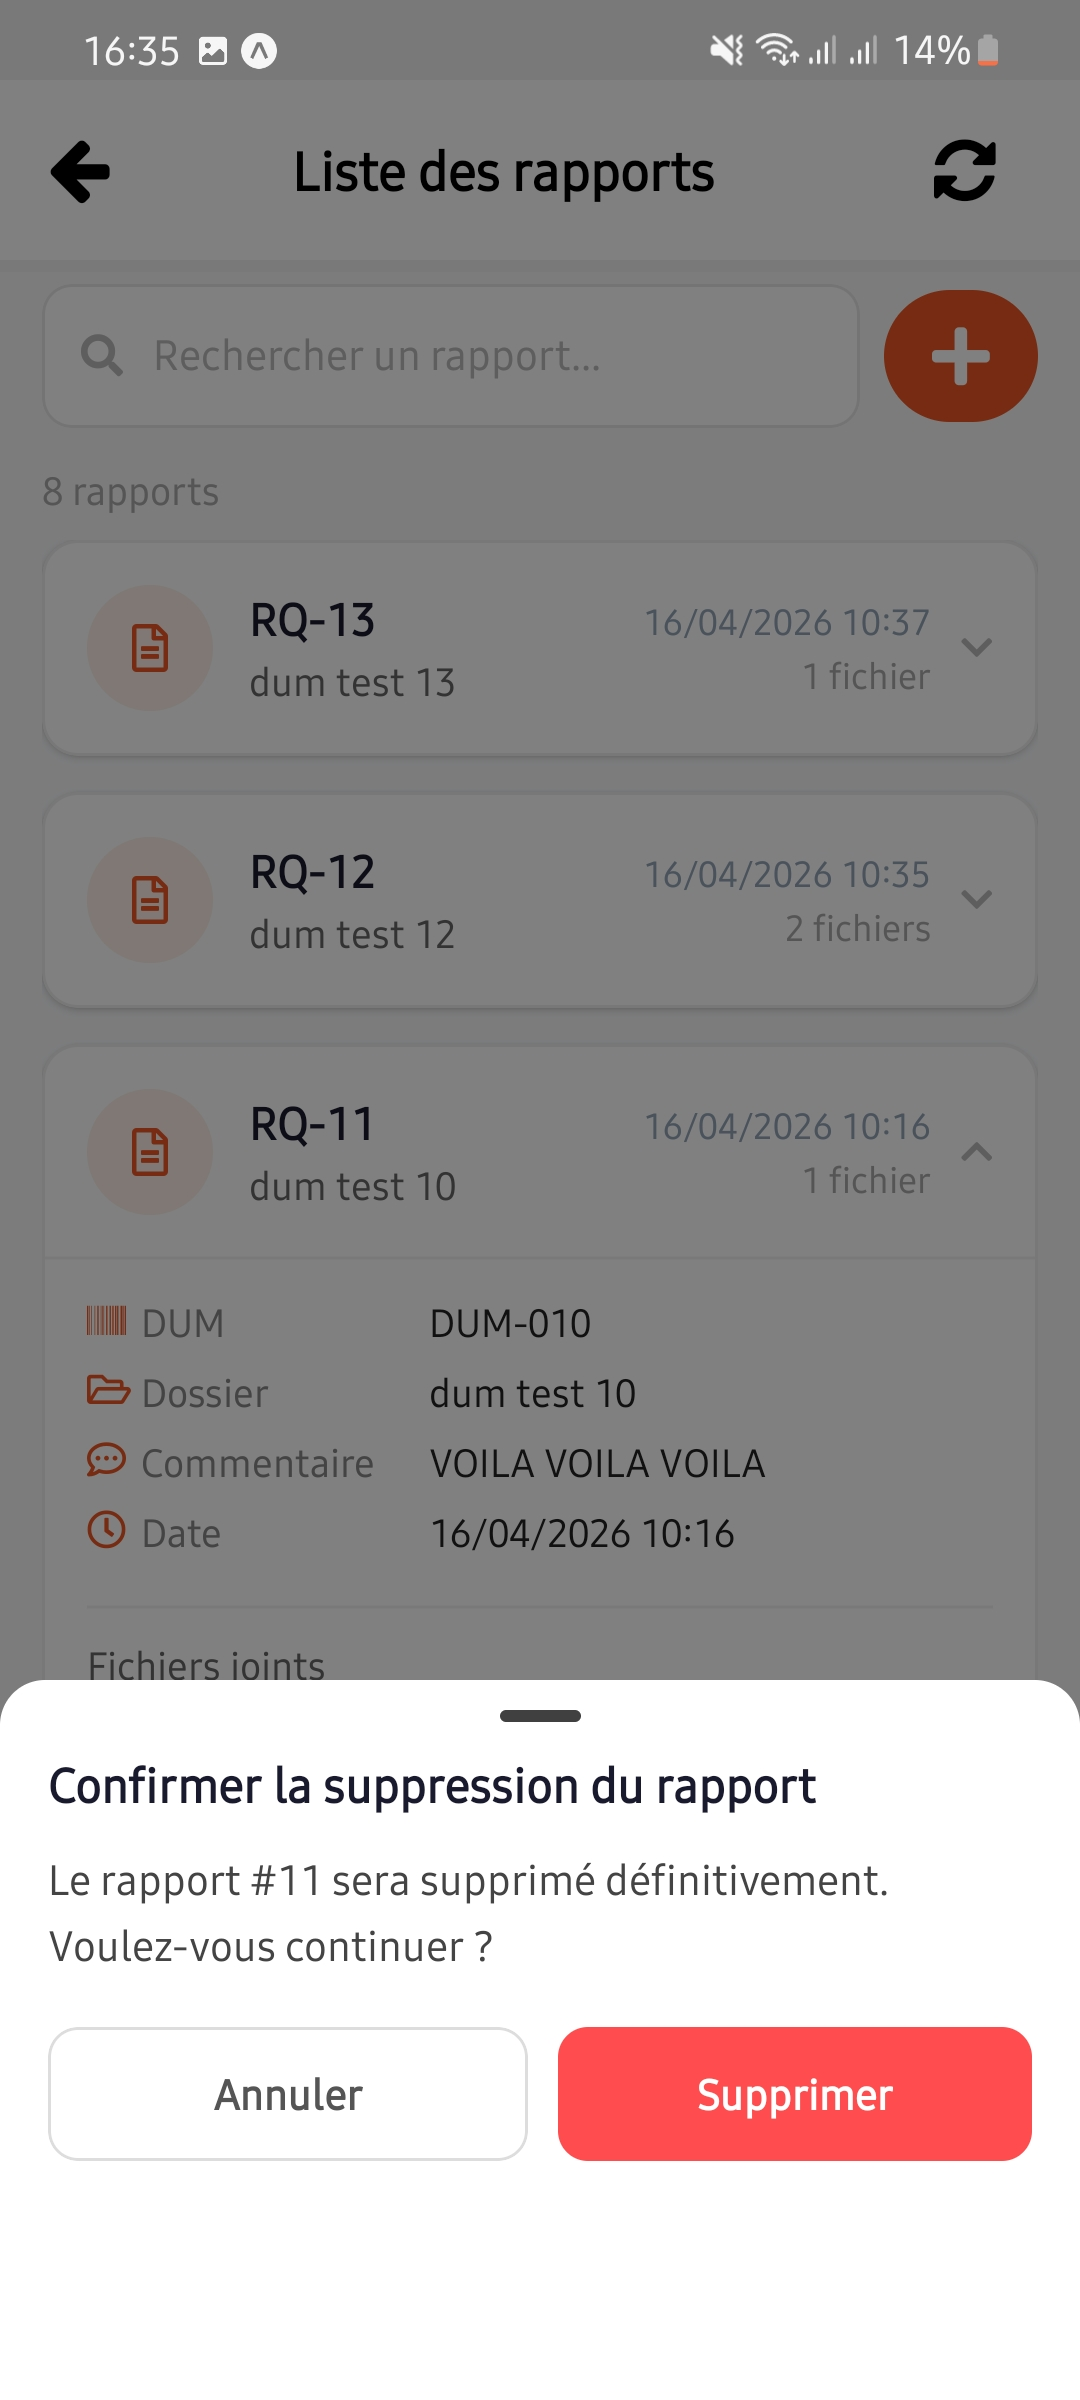
\includegraphics[width=0.85\textwidth]{assets/rapport-qualite-delete-confirm.jpg}
    }{
    \textit{Suppression : fichier assets/rapport-qualite-delete-confirm.jpg non trouvé.}
    }
    \caption{Confirmation de suppression d'un rapport}
    \label{fig:rapport-qualite-delete-confirm}
    \end{minipage}
    \end{figure}

    \subsection{Sprint 4 : Module Rotation et Module Lieux}

    \subsubsection{Module Rotation}

    Le module Rotation est un module en lecture seule qui affiche la liste paginée des rotations de véhicules. Chaque carte présente le véhicule, le chauffeur assigné, le kilométrage parcouru, la ville d'arrivée et un badge de disponibilité (Disponible en vert ou Réservé en rouge). Un bouton de filtre ouvre une feuille modale proposant quatre critères : chauffeur, véhicule, disponibilité et intervalle de dates.

    La Figure~\ref{fig:rotation-list} présente la liste des rotations, et la Figure~\ref{fig:rotation-filter} illustre la feuille de filtrage.

    \begin{figure}[ht]
    \centering
    \begin{minipage}[b]{0.45\textwidth}
    \centering
    \IfFileExists{assets/rotation-list.jpg}{
    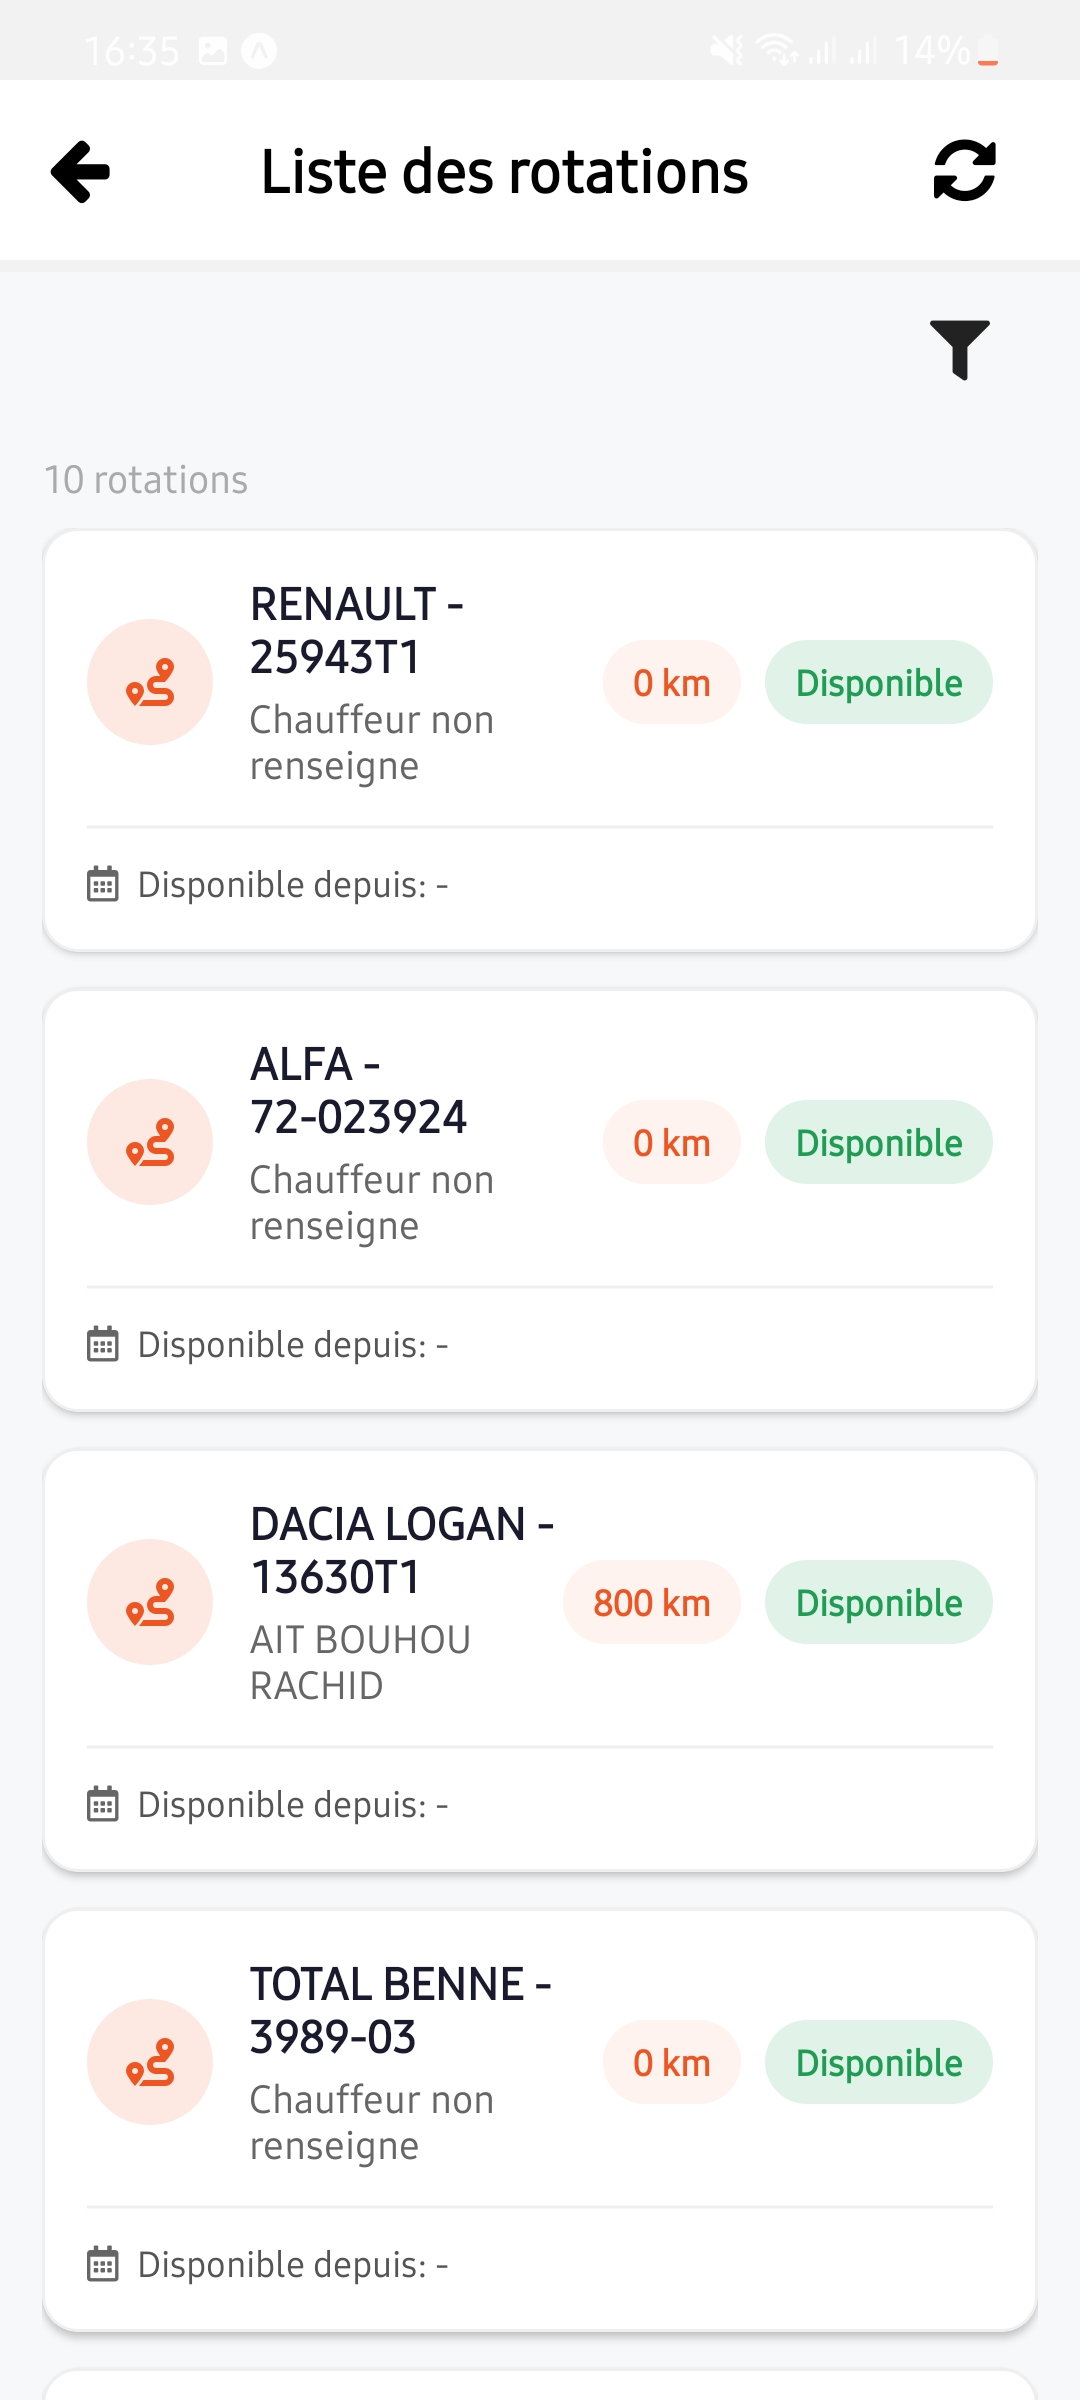
\includegraphics[width=0.85\textwidth]{assets/rotation-list.jpg}
    }{
    \textit{Liste des rotations : fichier assets/rotation-list.jpg non trouvé.}
    }
    \caption{Liste des rotations — véhicules et disponibilité}
    \label{fig:rotation-list}
    \end{minipage}\hfill
    \begin{minipage}[b]{0.45\textwidth}
    \centering
    \IfFileExists{assets/rotation-filter.jpg}{
    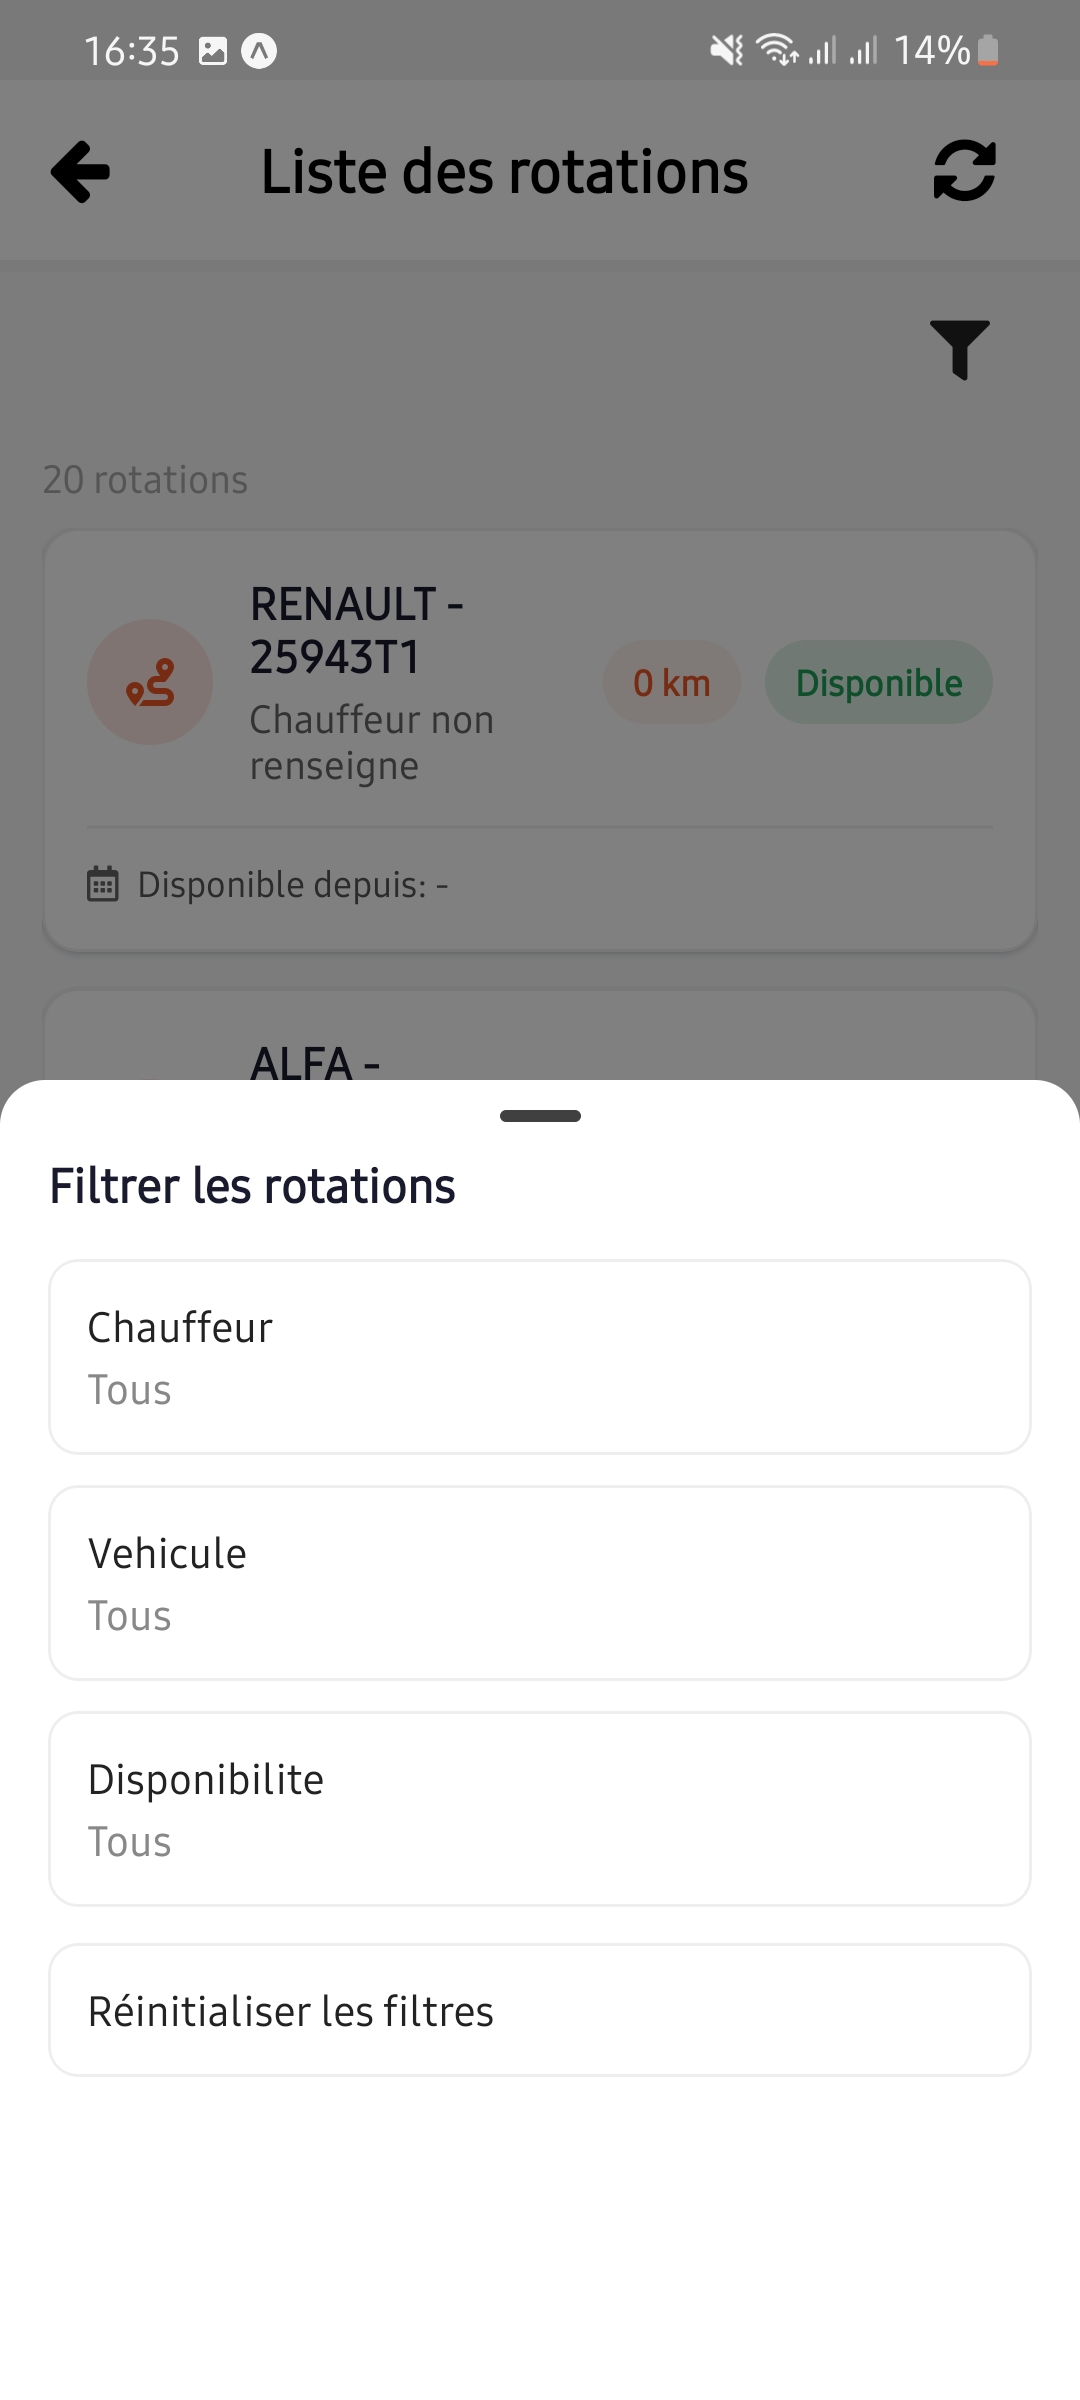
\includegraphics[width=0.85\textwidth]{assets/rotation-filter.jpg}
    }{
    \textit{Filtre : fichier assets/rotation-filter.jpg non trouvé.}
    }
    \caption{Feuille de filtrage — chauffeur, véhicule, disponibilité}
    \label{fig:rotation-filter}
    \end{minipage}
    \end{figure}

    \subsubsection{Module Lieux de projets}

    Le module Lieux de projets gère les chantiers et dépôts avec leurs coordonnées GPS, contacts et photos. L'écran principal affiche une liste filtrable par type (Chantier ou Dépôt). Chaque carte est expansive et dévoile les détails du lieu (contact, téléphone, coordonnées GPS, commentaire), une galerie de photos et des boutons d'action : ouvrir la localisation dans Google Maps, appeler le contact, ou modifier/supprimer le lieu.

    L'écran de création capture automatiquement les coordonnées GPS du terminal, propose un formulaire (type de projet, contact, téléphone, commentaire) et une zone de prise de photos ou sélection de fichiers.

    La Figure~\ref{fig:lieux-list} montre la liste des lieux, la Figure~\ref{fig:lieux-card-expanded} illustre la carte expansive, et la Figure~\ref{fig:lieux-create} présente l'écran de création.

    \begin{figure}[ht]
    \centering
    \begin{minipage}[b]{0.32\textwidth}
    \centering
    \IfFileExists{assets/lieux-list.jpg}{
    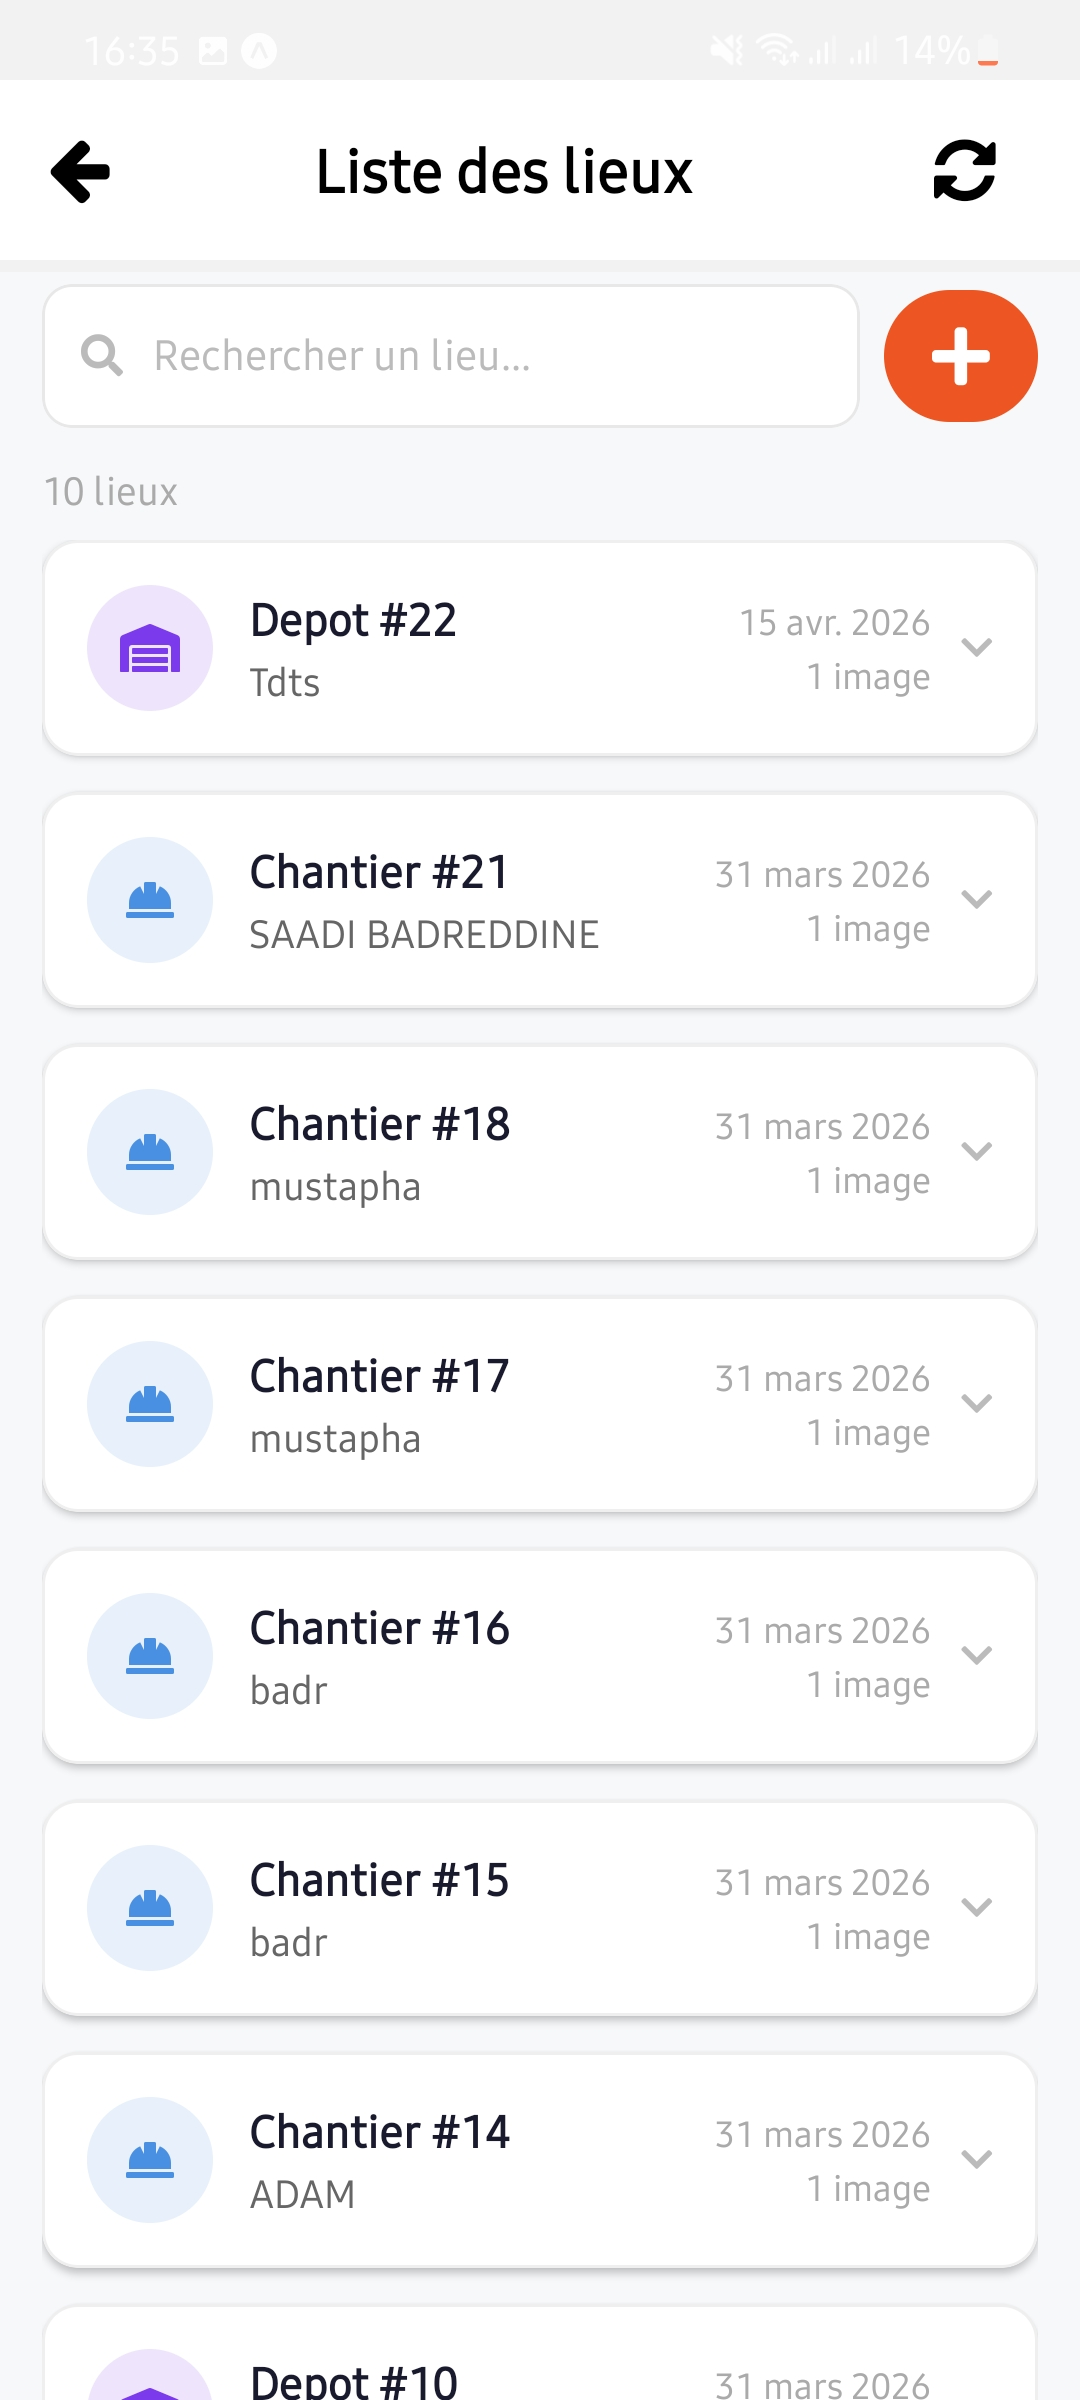
\includegraphics[width=\textwidth]{assets/lieux-list.jpg}
    }{
    \textit{Liste des lieux : fichier assets/lieux-list.jpg non trouvé.}
    }
    \caption{Liste des lieux — chantiers et dépôts}
    \label{fig:lieux-list}
    \end{minipage}\hfill
    \begin{minipage}[b]{0.32\textwidth}
    \centering
    \IfFileExists{assets/lieux-card-expanded.jpg}{
    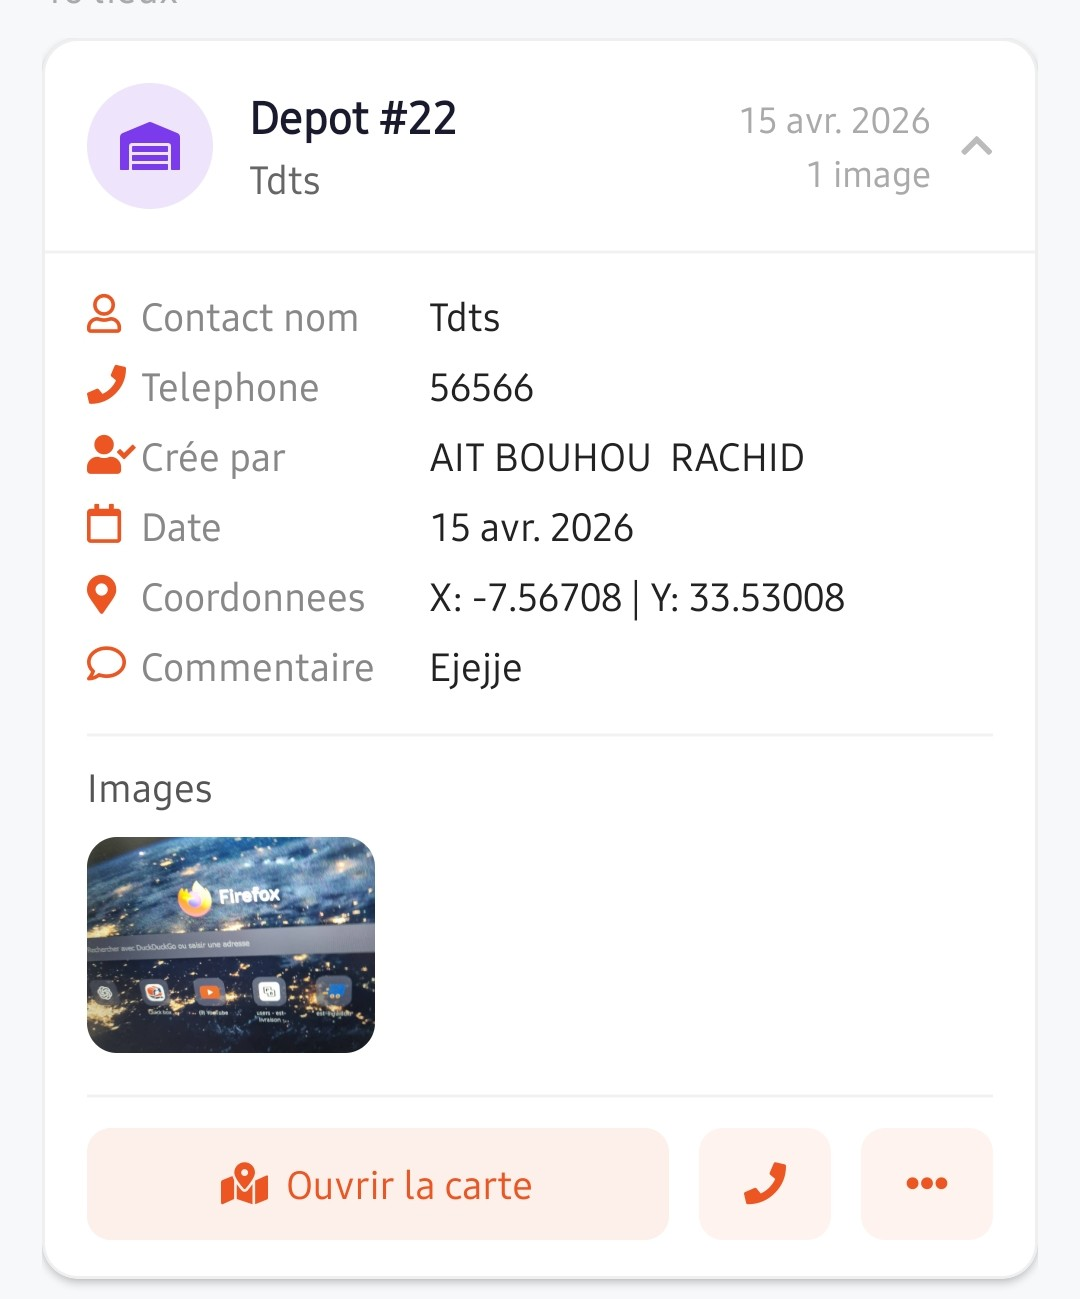
\includegraphics[width=\textwidth]{assets/lieux-card-expanded.jpg}
    }{
    \textit{Carte expansive : fichier assets/lieux-card-expanded.jpg non trouvé.}
    }
    \caption{Carte expansive — détails et galerie}
    \label{fig:lieux-card-expanded}
    \end{minipage}\hfill
    \begin{minipage}[b]{0.32\textwidth}
    \centering
    \IfFileExists{assets/lieux-create.jpg}{
    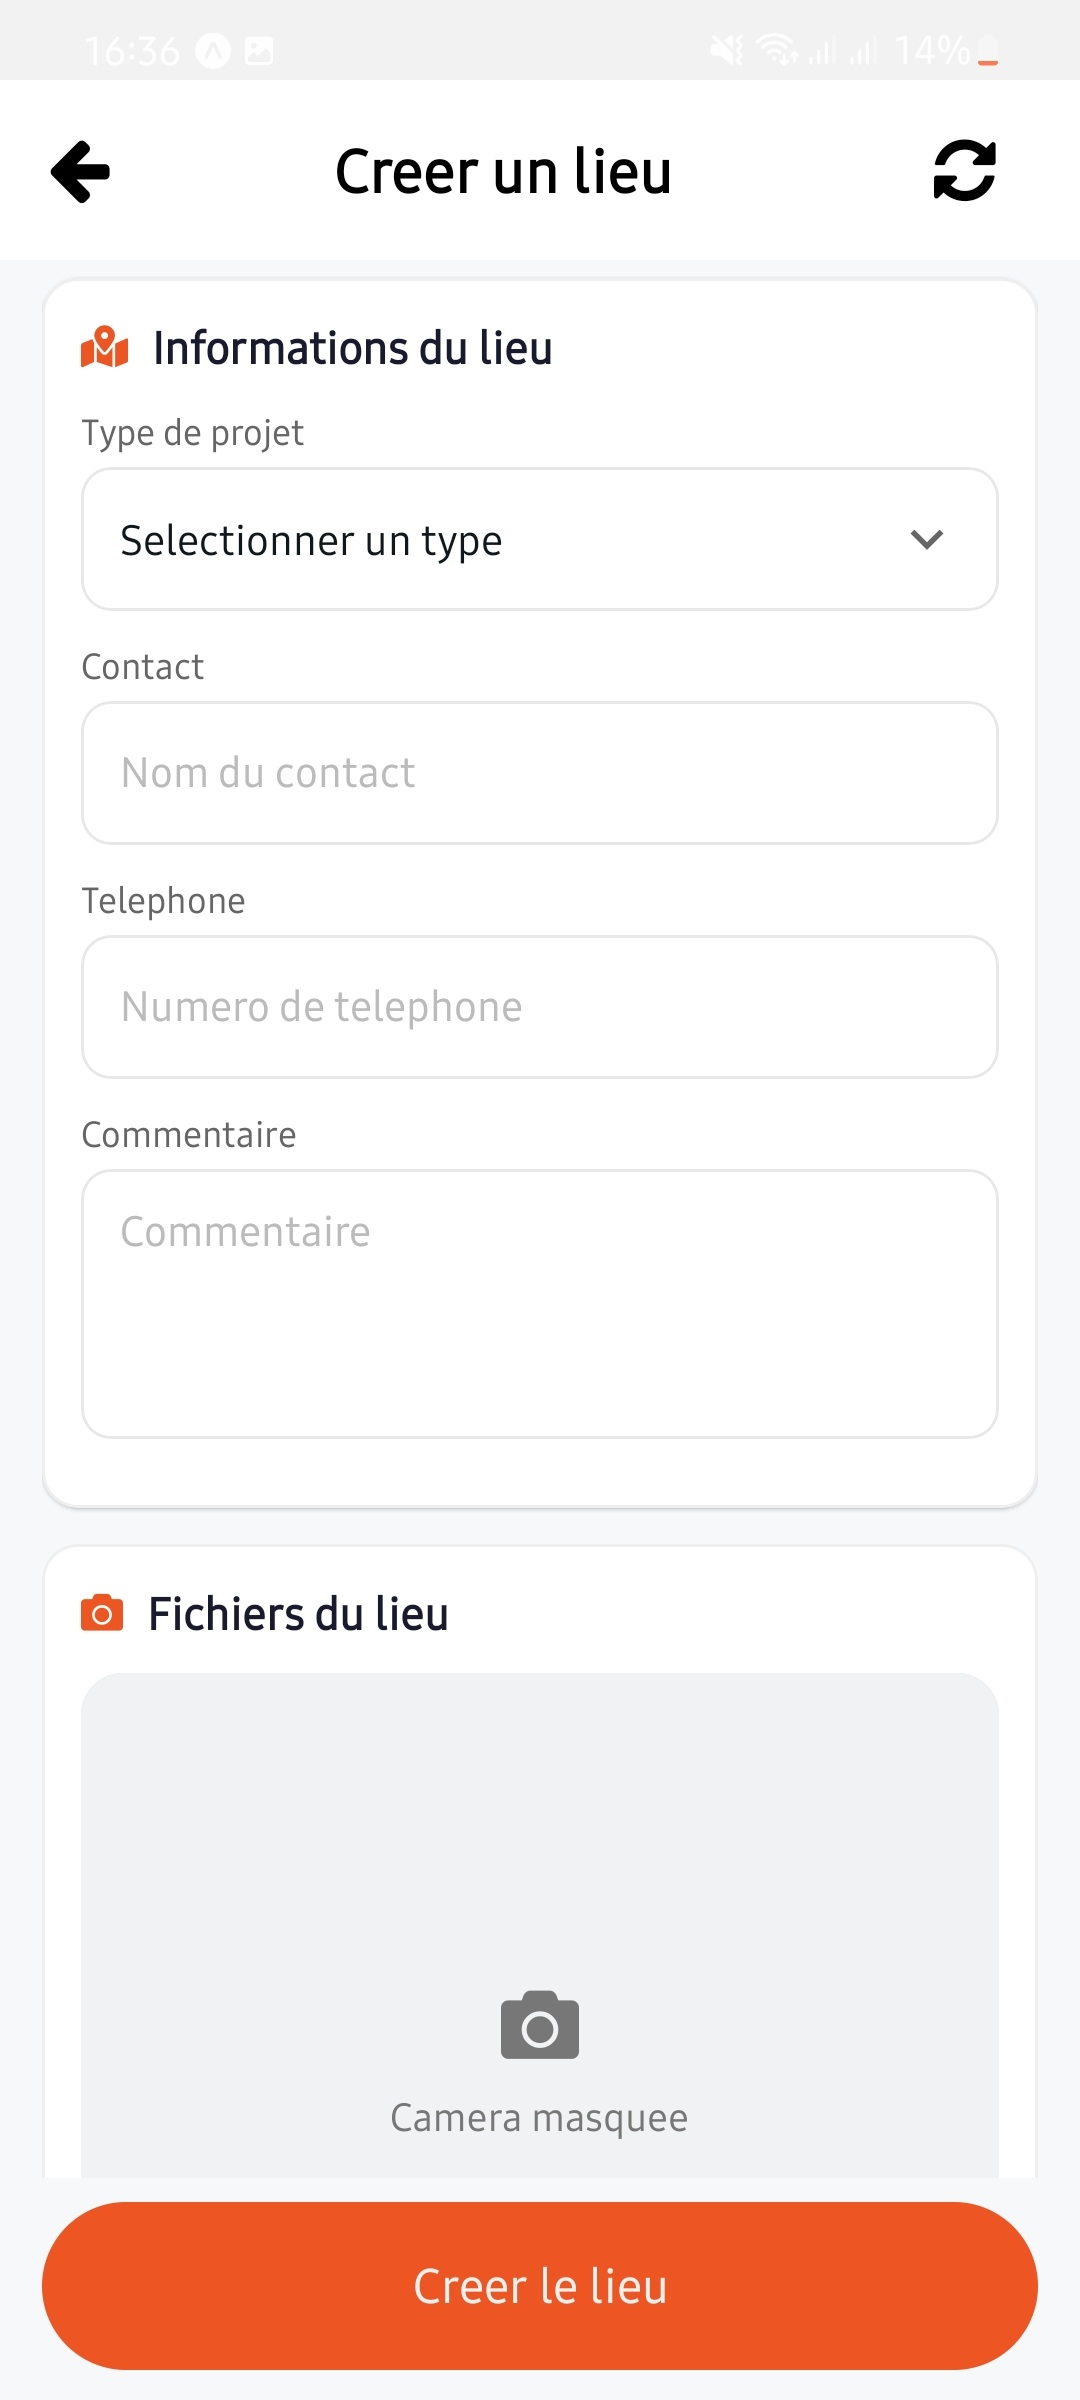
\includegraphics[width=\textwidth]{assets/lieux-create.jpg}
    }{
    \textit{Création : fichier assets/lieux-create.jpg non trouvé.}
    }
    \caption{Création d'un lieu — formulaire et GPS}
    \label{fig:lieux-create}
    \end{minipage}
    \end{figure}

    \subsection{Sprint 5 : Module Demande de transfert}

    Le module Demande de transfert gère les demandes de transfert de produits entre dépôts. Chaque demande comporte une référence, un dépôt source, un dépôt destination, un transporteur, une matricule, un numéro DUM, un statut et une observation. Les produits et lots associés à la demande suivent un cycle de préparation : un produit ou un lot peut être marqué comme préparé une fois vérifié. L'accès est contrôlé par quatre permissions : \texttt{LIST}, \texttt{CREATE}, \texttt{UPDATE} et \texttt{DELETE}.

    \subsubsection{Liste des demandes et carte expansive}

    L'écran principal affiche la liste paginée des demandes de transfert sous forme de cartes. Chaque carte présente la référence, le transporteur, un badge de statut coloré (vert pour Validé/Terminé, ambre pour Brouillon/En cours, rouge pour Refusé/Annulé) et la date. En appuyant sur une carte, des détails supplémentaires apparaissent : transporteur, matricule, DUM, dépôt source, dépôt destination, observation et créateur. Un bouton \og Détails \fg{} permet de naviguer vers l'écran de détail complet.

    La Figure~\ref{fig:dt-list} présente la liste des demandes, et la Figure~\ref{fig:dt-card-expanded} illustre la carte expansive avec les informations détaillées.

    \begin{figure}[ht]
    \centering
    \begin{minipage}[b]{0.45\textwidth}
    \centering
    \IfFileExists{assets/dt-list.jpg}{
    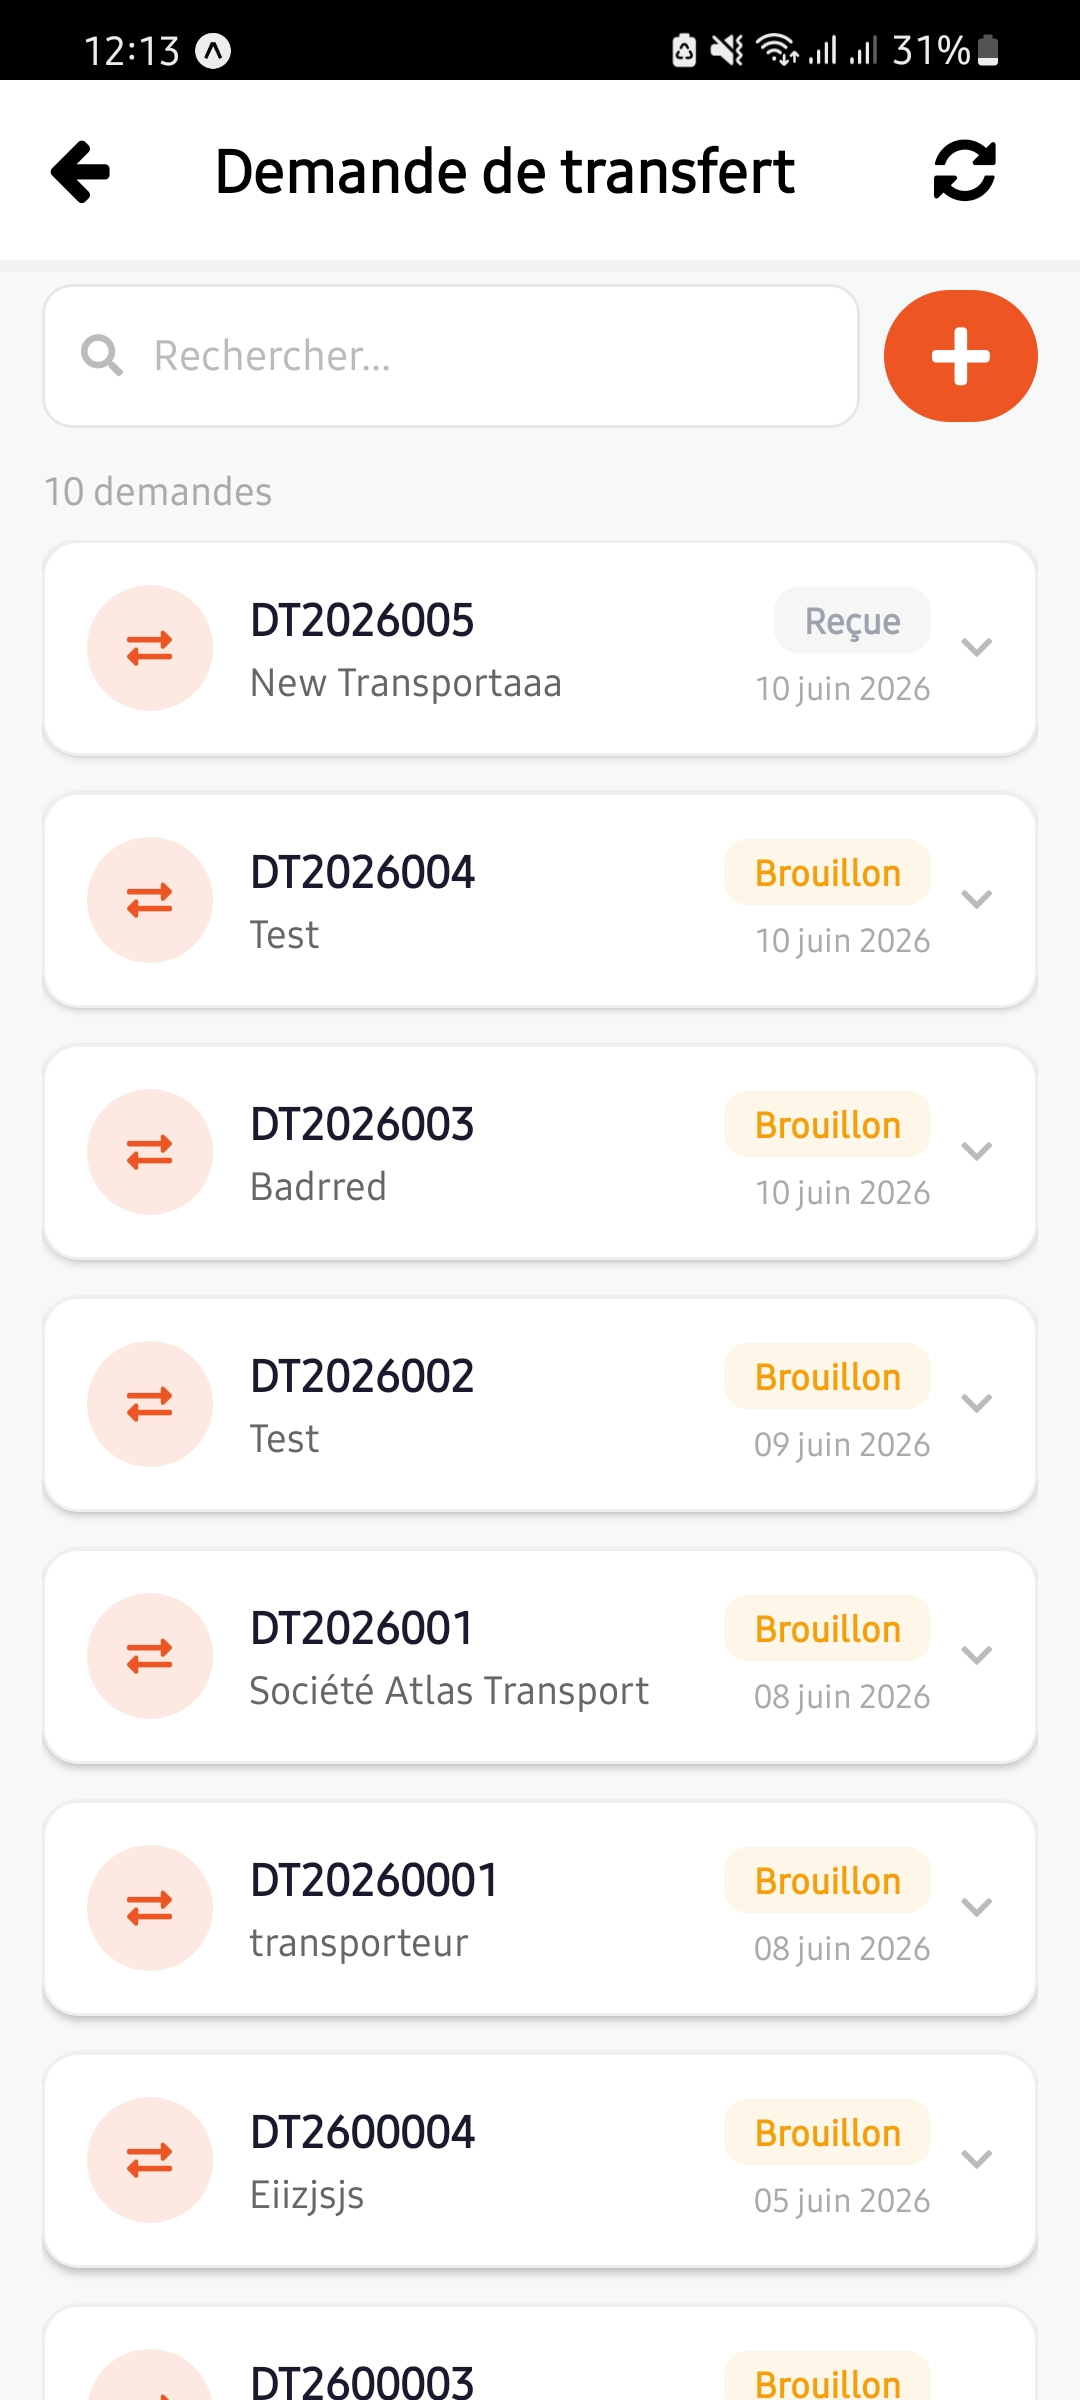
\includegraphics[width=0.85\textwidth]{assets/dt-list.jpg}
    }{
    \textit{Liste des demandes : fichier assets/dt-list.jpg non trouvé.}
    }
    \caption{Liste des demandes de transfert}
    \label{fig:dt-list}
    \end{minipage}\hfill
    \begin{minipage}[b]{0.45\textwidth}
    \centering
    \IfFileExists{assets/dt-card-expanded.jpg}{
    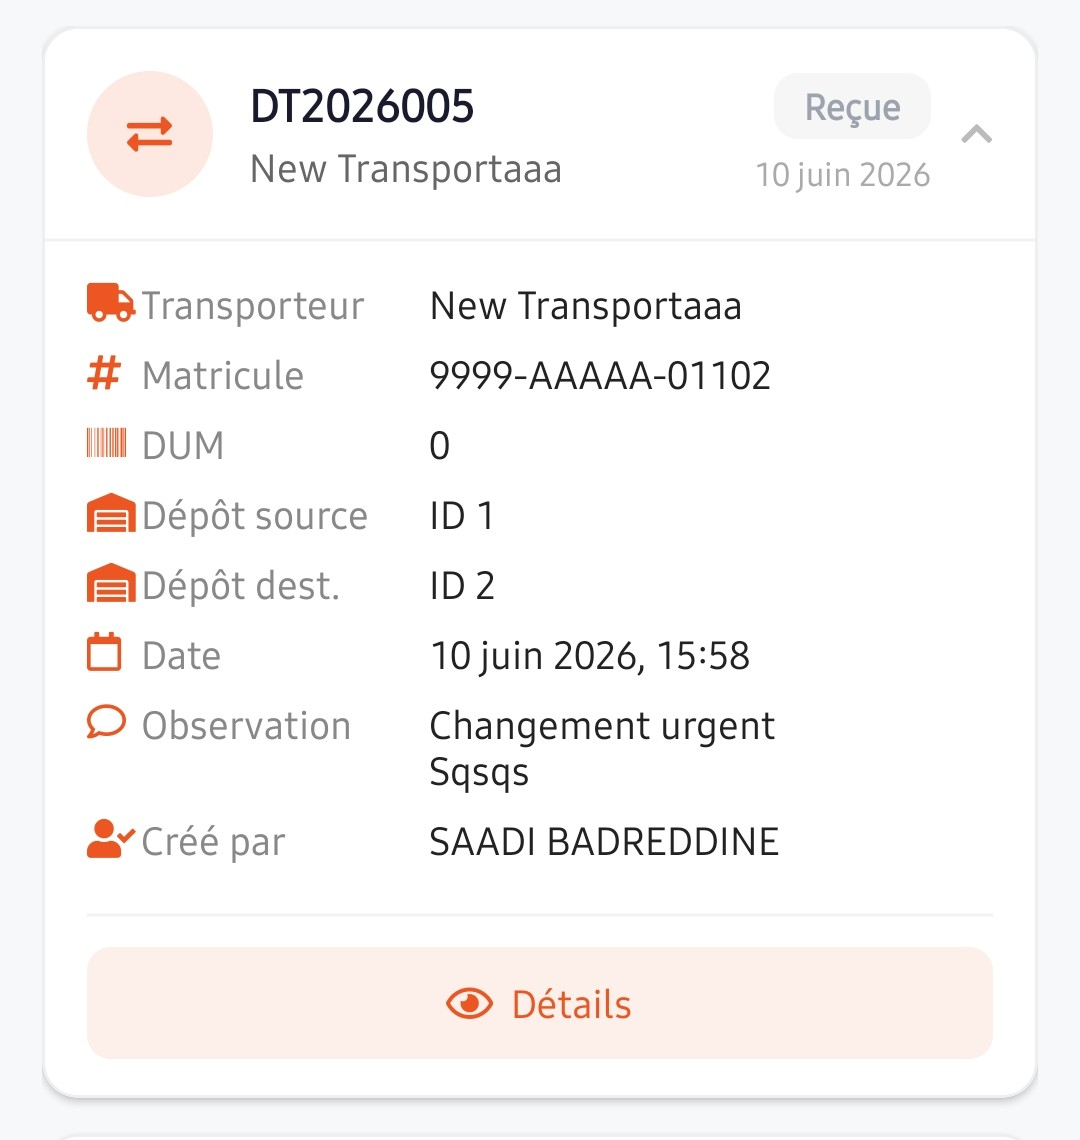
\includegraphics[width=0.85\textwidth]{assets/dt-card-expanded.jpg}
    }{
    \textit{Carte expansive : fichier assets/dt-card-expanded.jpg non trouvé.}
    }
    \caption{Carte de demande expansive — détails}
    \label{fig:dt-card-expanded}
    \end{minipage}
    \end{figure}

    \subsubsection{Écran de détail}

    L'écran de détail affiche trois sections principales. La première est une carte d'en-tête avec la référence de la demande, un badge de statut modifiable par un appui (ouvrant un sélecteur de statut à quatre choix : Brouillon, En cours, Envoyé, Reçue), puis les champs Dépôt source, Dépôt destination, Transporteur, Matricule, DUM, Date, Observation et Créé par. Deux boutons d'action conditionnels apparaissent sous l'en-tête : Modifier (si permission \texttt{UPDATE}) et Supprimer (si permission \texttt{DELETE}).

    La deuxième section liste les produits associés à la demande. Chaque produit affiche son nom, le nombre de FDX, la quantité, l'unité et un badge de préparation (Préparé / Non préparé). Si le produit n'est pas encore préparé et que l'utilisateur dispose de la permission \texttt{UPDATE}, deux boutons d'action apparaissent : Gérer les lots (ouvrant la feuille de sélection des lots) et Supprimer le produit. Si des lots sont associés au produit, ils sont listés avec leur numéro de lot, leur propre badge de préparation, et des détails expansibles (code lot, lot ancien, quantité, nombre de pièces, longueur, date d'entrée, dépôt).

    La Figure~\ref{fig:dt-details} présente l'écran de détail complet avec la carte d'en-tête, le sélecteur de statut et la liste des produits.

    \begin{figure}[ht]
    \centering
    \IfFileExists{assets/dt-details.jpg}{
    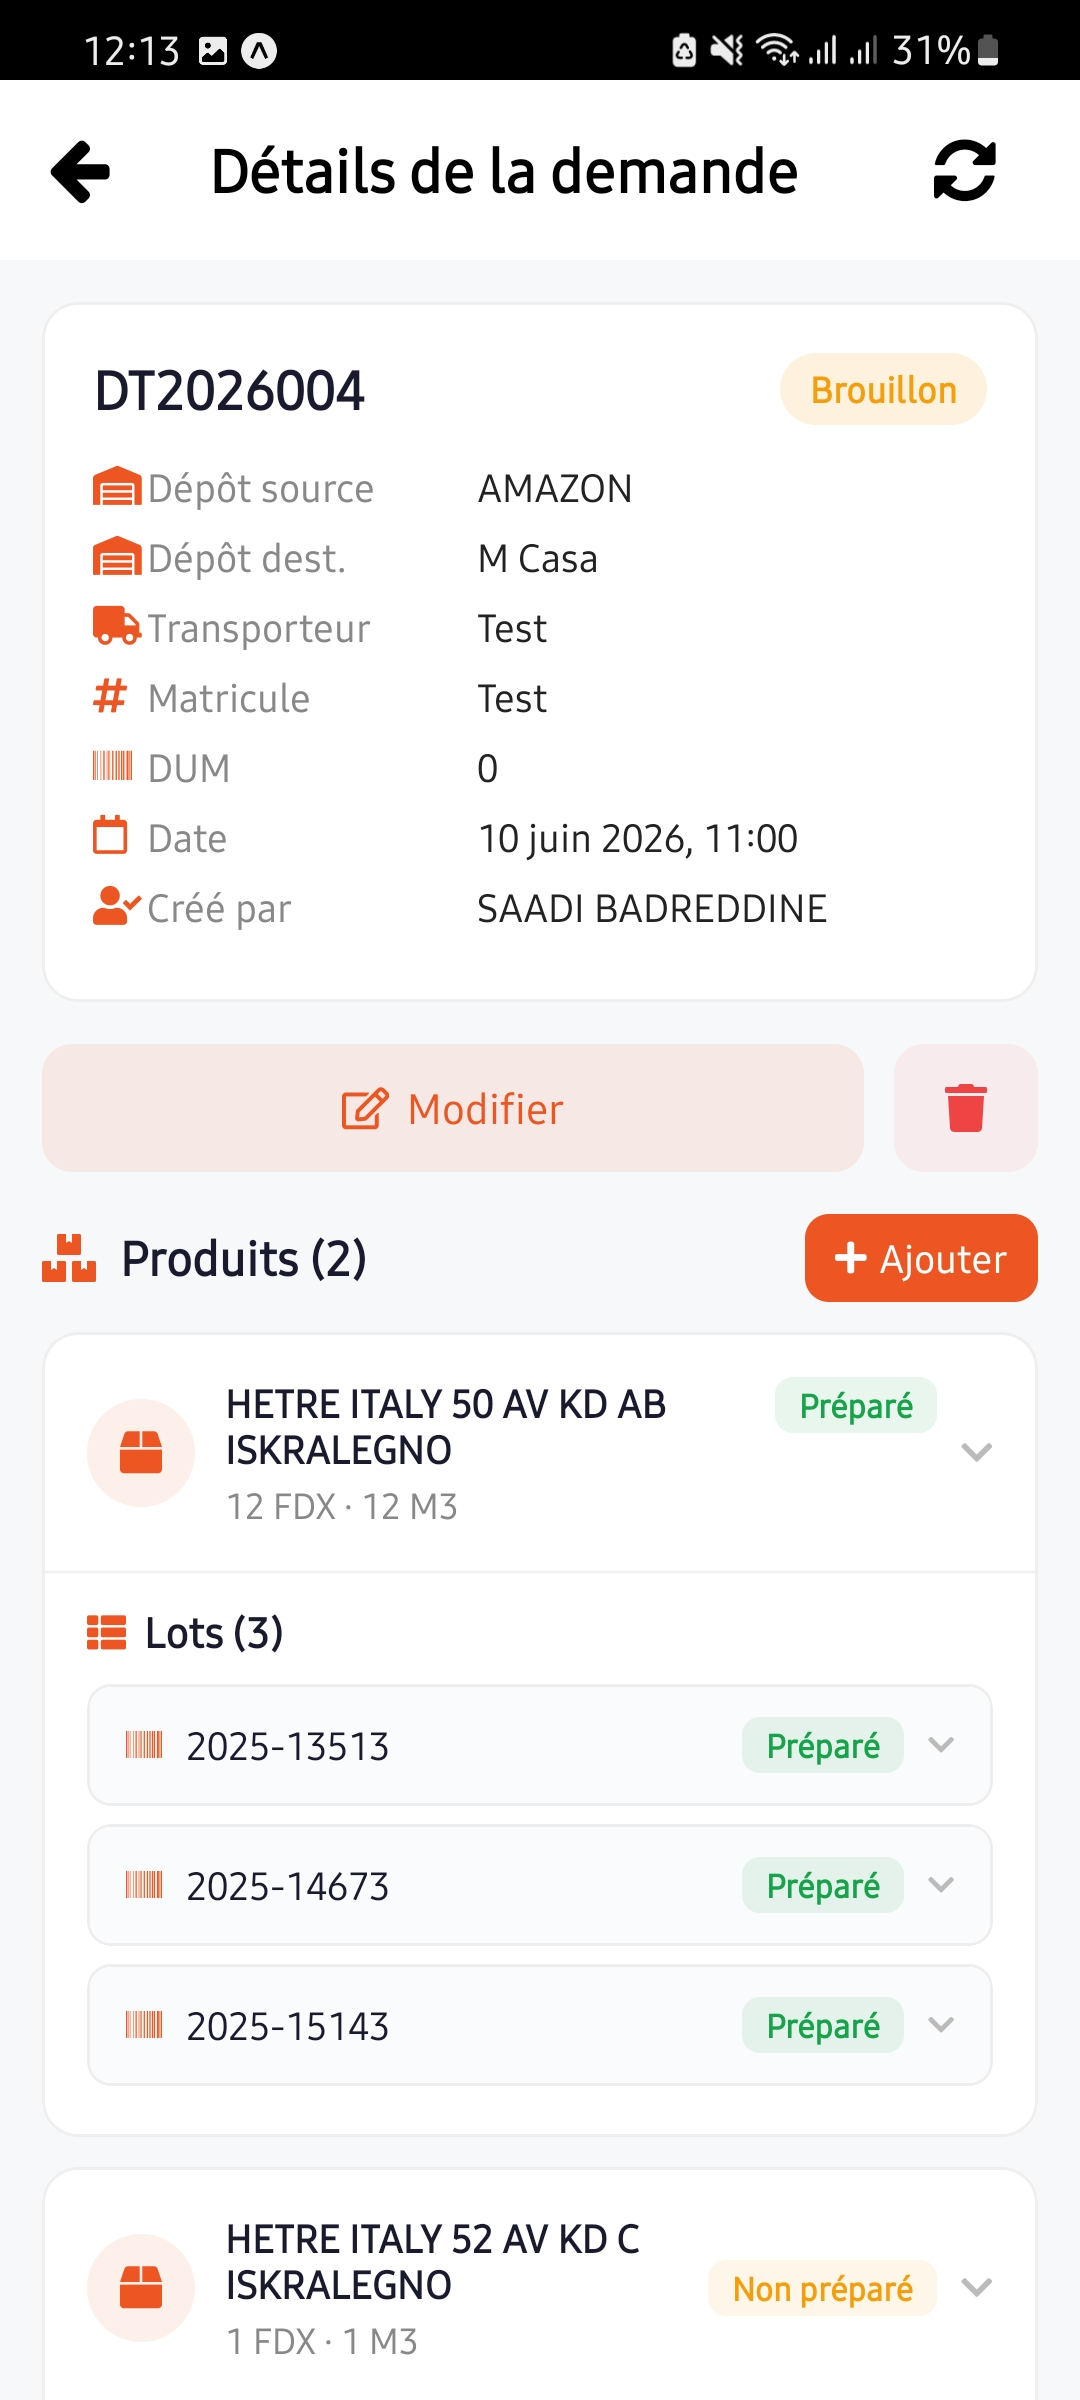
\includegraphics[width=0.35\textwidth]{assets/dt-details.jpg}
    }{
    \textit{Écran de détail : fichier assets/dt-details.jpg non trouvé.}
    }
    \caption{Écran de détail — en-tête, statut et produits}
    \label{fig:dt-details}
    \end{figure}

    \subsubsection{Suppression, gestion des lots et préparation}

    La suppression d'une demande de transfert affiche une feuille de confirmation : \og La demande de transfert "\{référence\}" sera supprimée définitivement. Voulez-vous continuer ? \fg{}, avec les boutons Annuler et Supprimer.

    La gestion des lots (\og Gérer les lots \fg{}) permet de sélectionner ou désélectionner les lots à associer à un produit. La feuille affiche la liste de tous les lots disponibles pour le produit, chacun avec une case à cocher, son numéro de lot, des badges (Préparé en vert, Actuel en bleu) et les informations de détail (quantité, pièces, dépôt, date). Les lots déjà préparés ne sont pas modifiables. Un compteur en bas indique le nombre de lots sélectionnés et un bouton Enregistrer enregistre les modifications.

    La préparation d'un produit ou d'un lot affiche une feuille de confirmation demandant de valider le passage au statut Préparé. Le bouton de confirmation est vert pour l'acceptation.

    La Figure~\ref{fig:dt-delete} présente la confirmation de suppression, la Figure~\ref{fig:dt-manage-lots} illustre la feuille de gestion des lots, la Figure~\ref{fig:dt-preparer-produit} montre la confirmation de préparation d'un produit, et la Figure~\ref{fig:dt-preparer-lot} celle d'un lot.

    \begin{figure}[H]
    \centering
    \begin{minipage}[b]{0.38\textwidth}
    \centering
    \IfFileExists{assets/dt-delete.jpg}{
    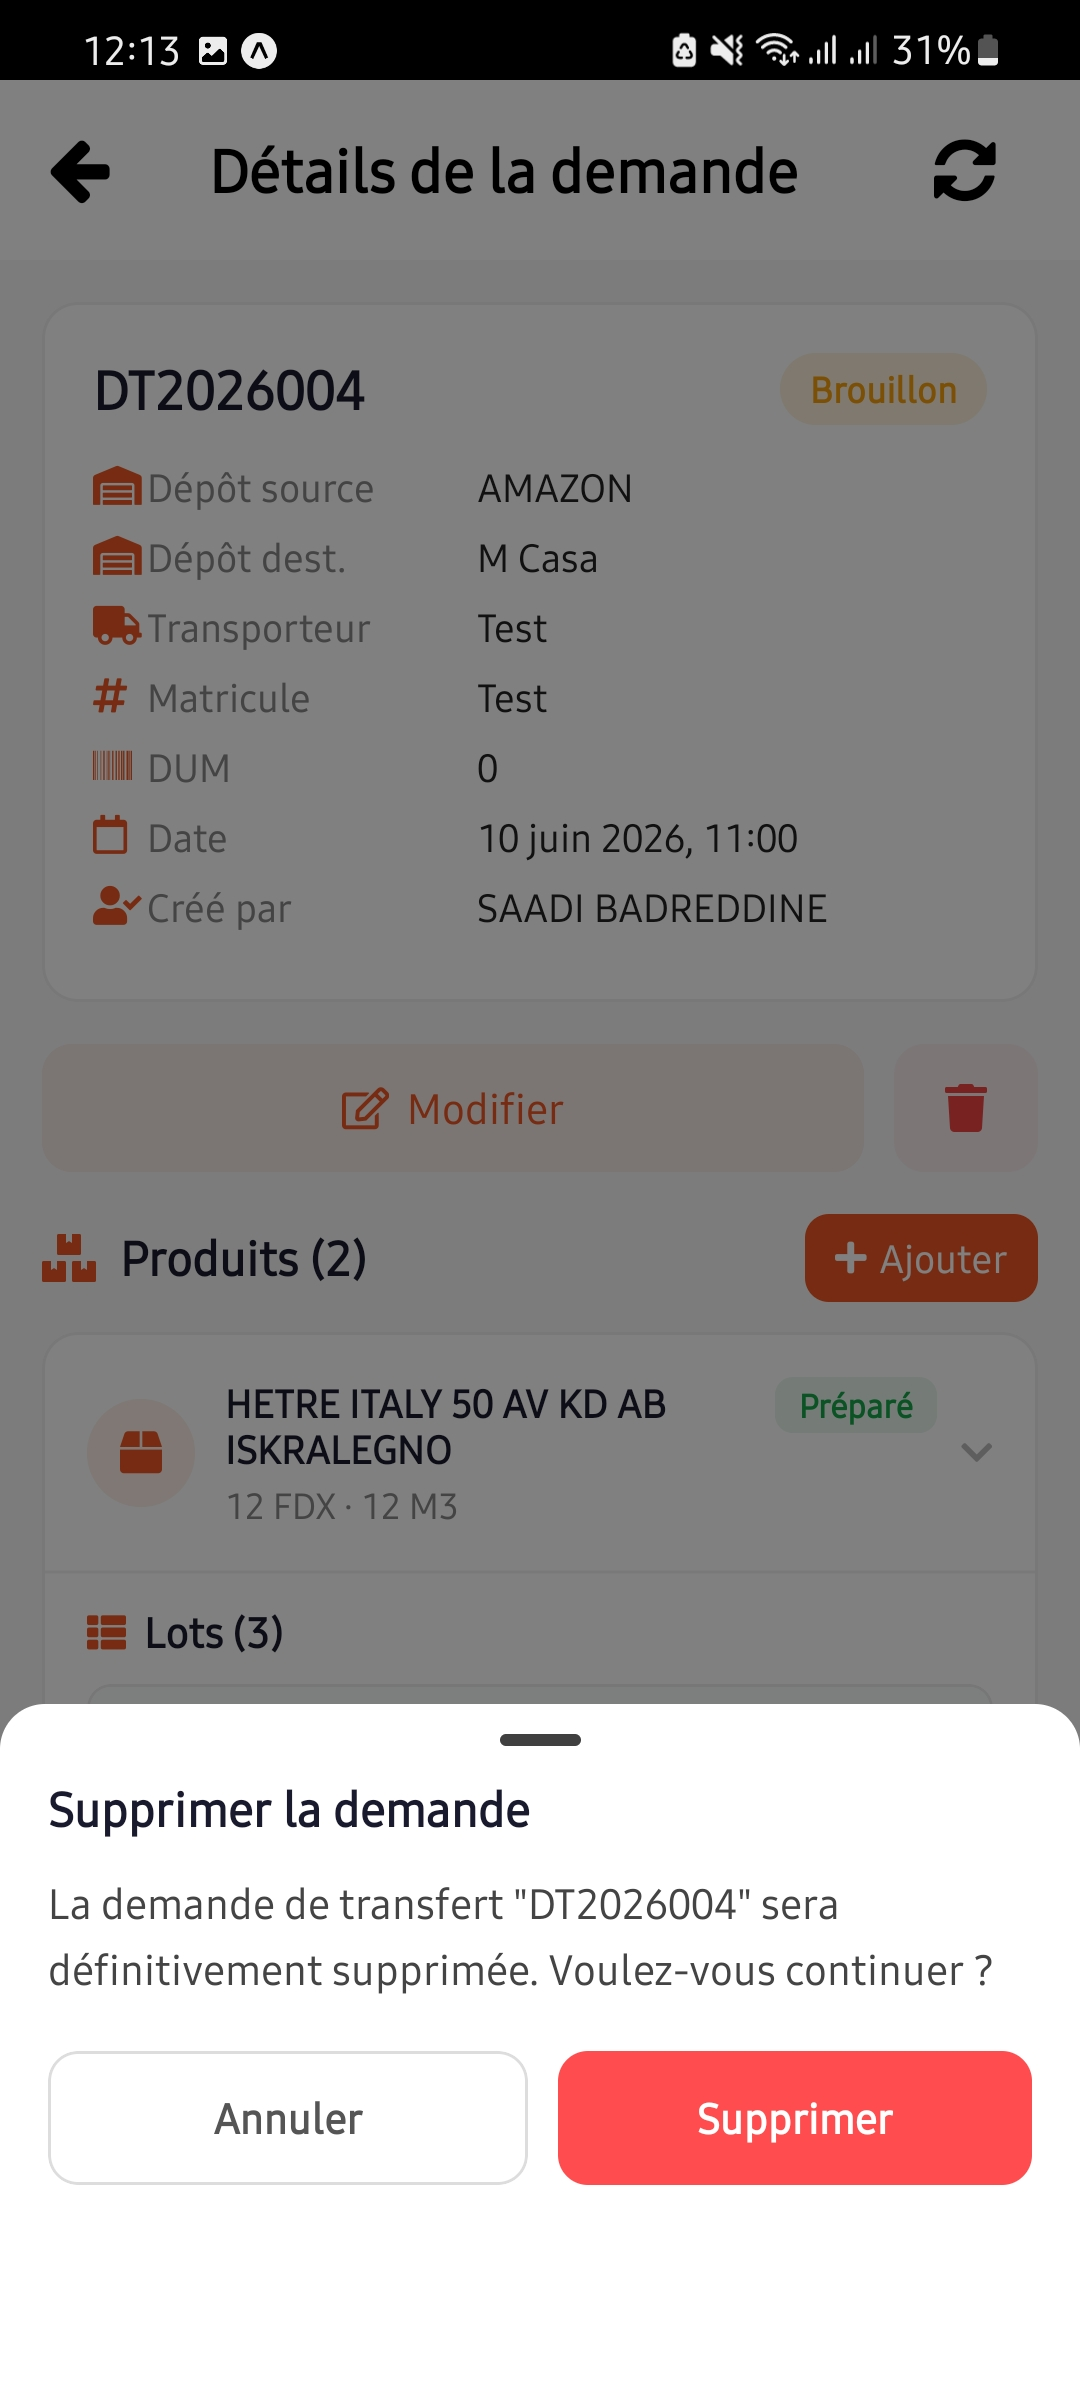
\includegraphics[width=0.75\textwidth]{assets/dt-delete.jpg}
    }{
    \textit{Suppression : fichier assets/dt-delete.jpg non trouvé.}
    }
    \caption{Confirmation de suppression}
    \label{fig:dt-delete}
    \end{minipage}\hfill
    \begin{minipage}[b]{0.38\textwidth}
    \centering
    \IfFileExists{assets/dt-manage-lots.jpg}{
    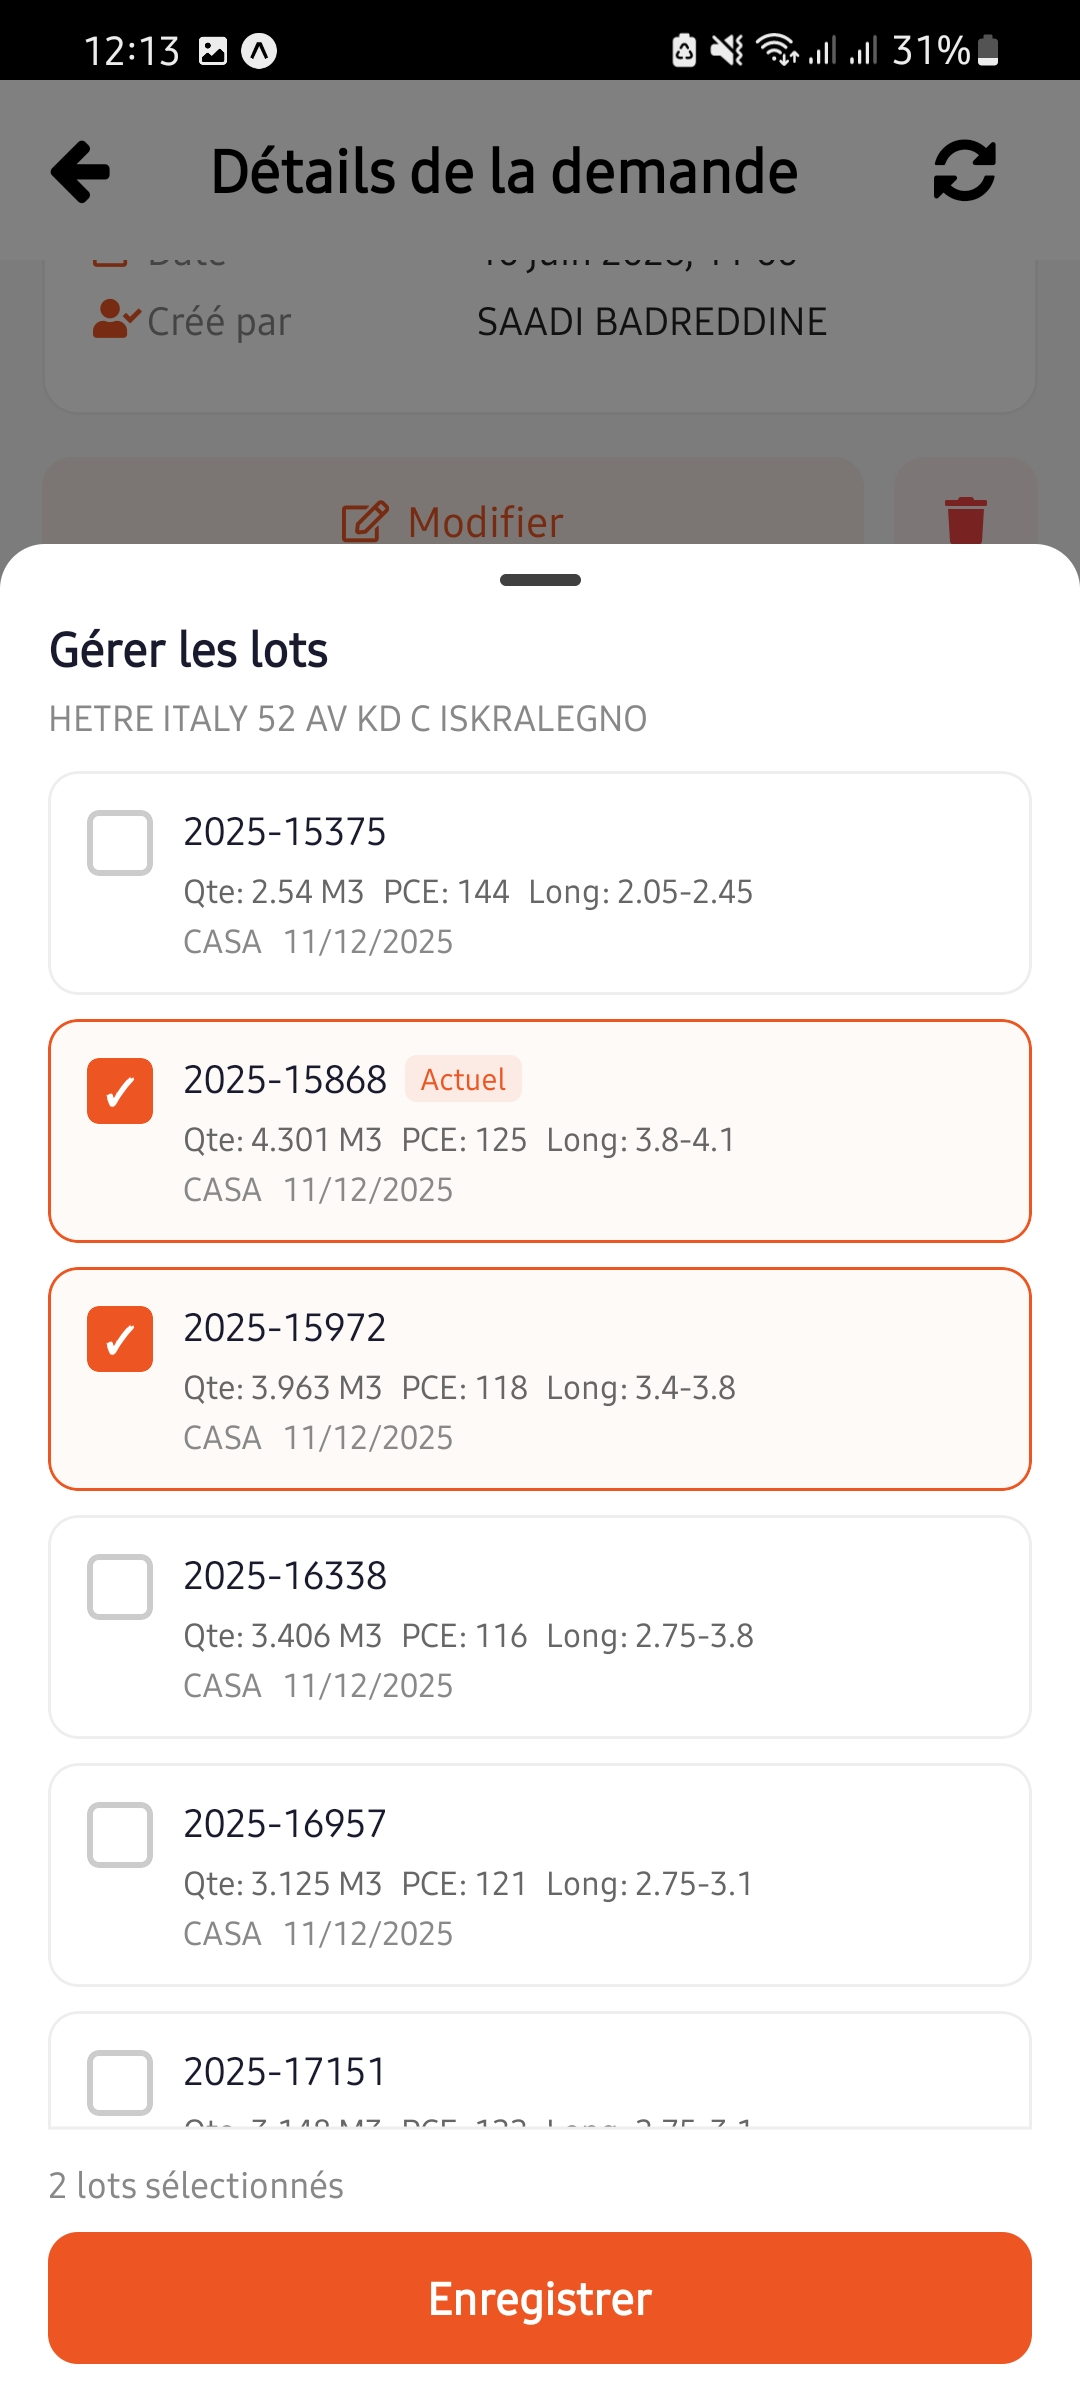
\includegraphics[width=0.75\textwidth]{assets/dt-manage-lots.jpg}
    }{
    \textit{Gestion des lots : fichier assets/dt-manage-lots.jpg non trouvé.}
    }
    \caption{Gérer les lots — sélection et badges}
    \label{fig:dt-manage-lots}
    \end{minipage}
    \end{figure}

    \begin{figure}[H]
    \centering
    \begin{minipage}[b]{0.38\textwidth}
    \centering
    \IfFileExists{assets/dt-preparer-produit.jpg}{
    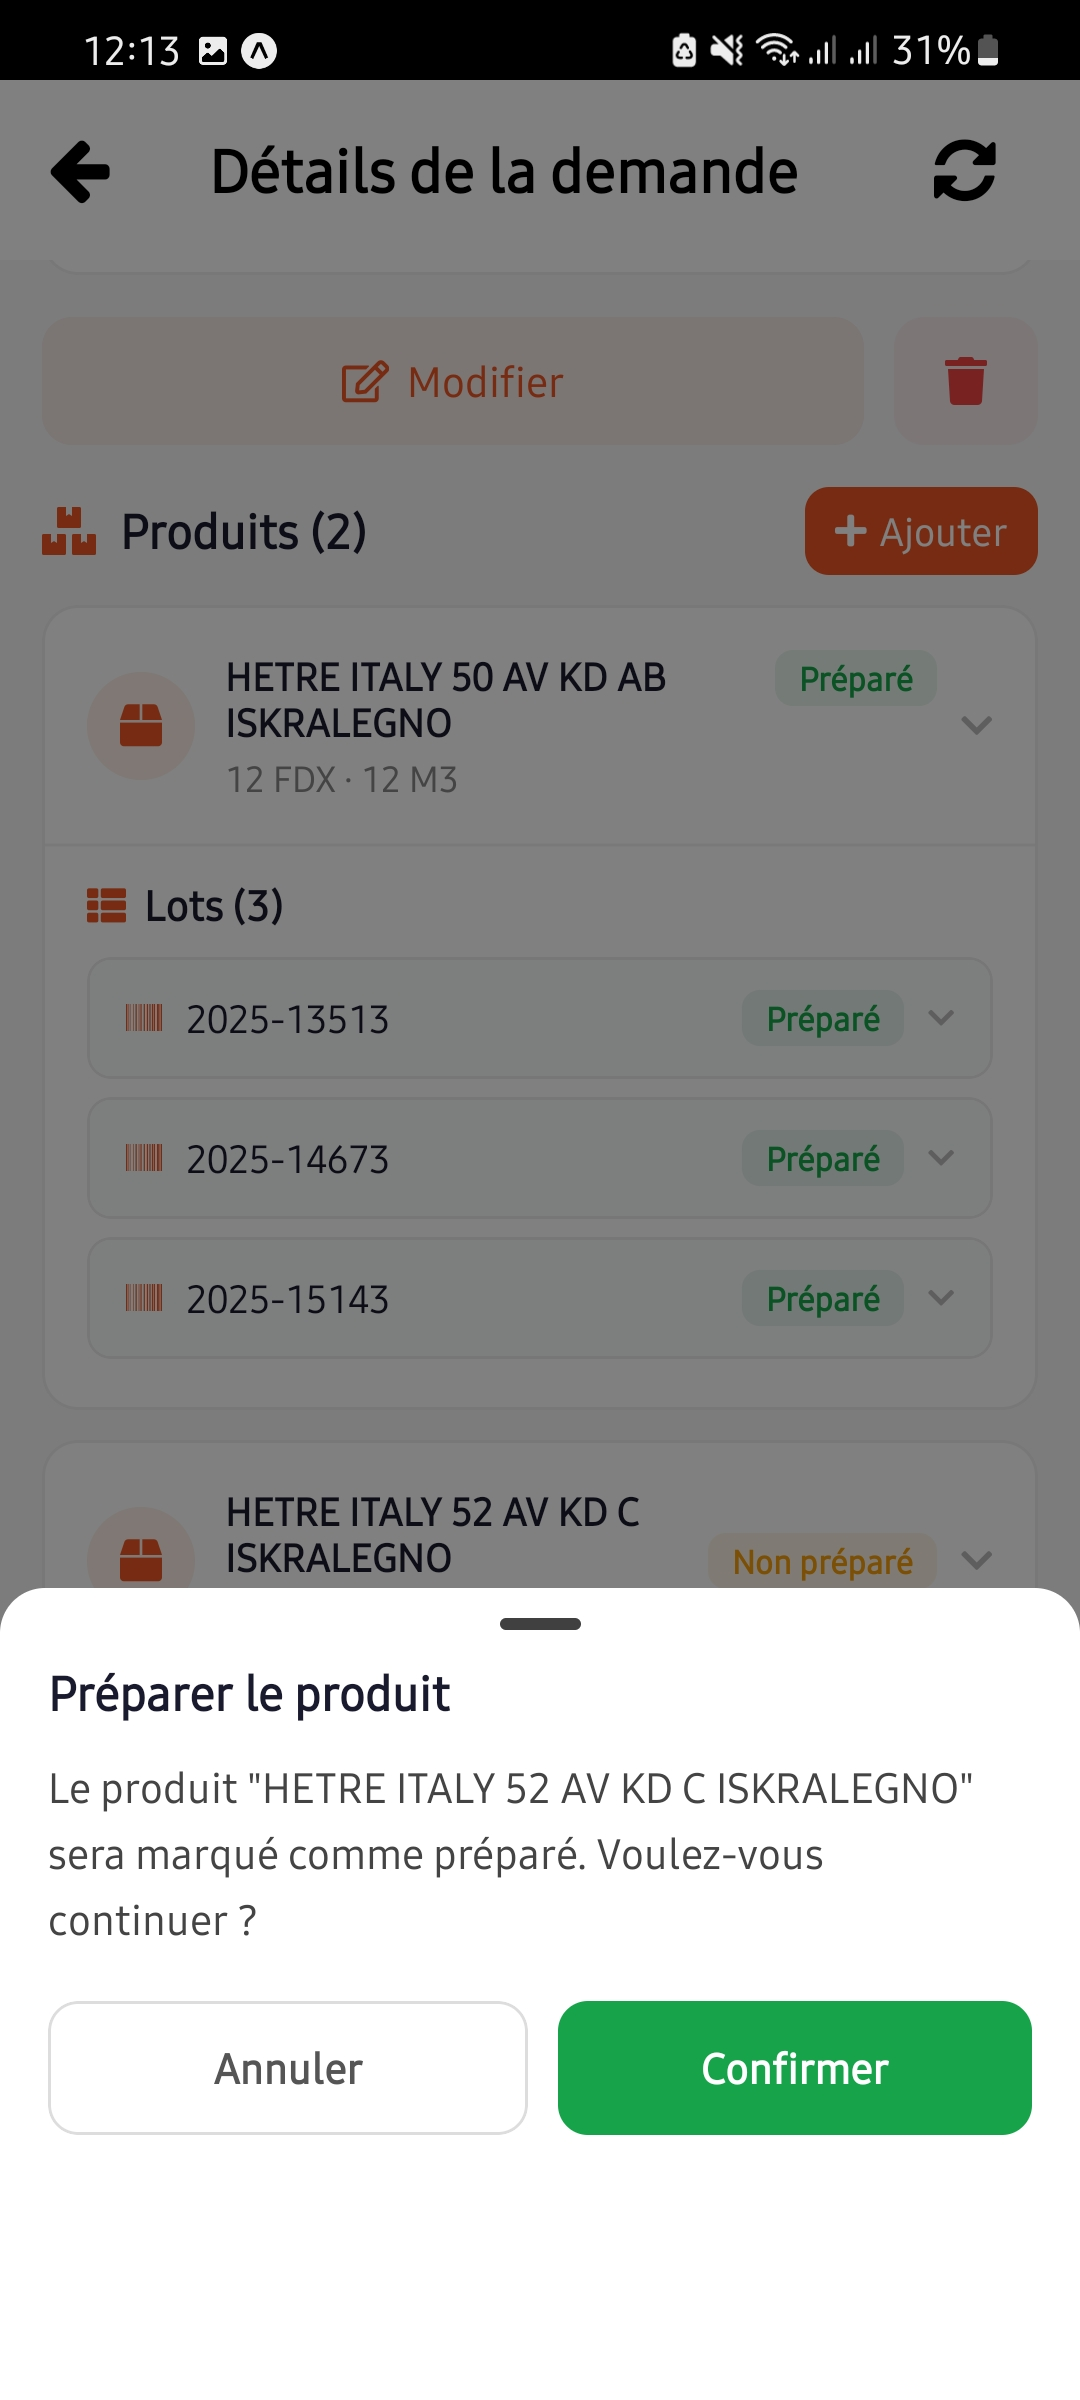
\includegraphics[width=0.75\textwidth]{assets/dt-preparer-produit.jpg}
    }{
    \textit{Préparation produit : fichier assets/dt-preparer-produit.jpg non trouvé.}
    }
    \caption{Préparer un produit}
    \label{fig:dt-preparer-produit}
    \end{minipage}\hfill
    \begin{minipage}[b]{0.38\textwidth}
    \centering
    \IfFileExists{assets/dt-preparer-lot.jpg}{
    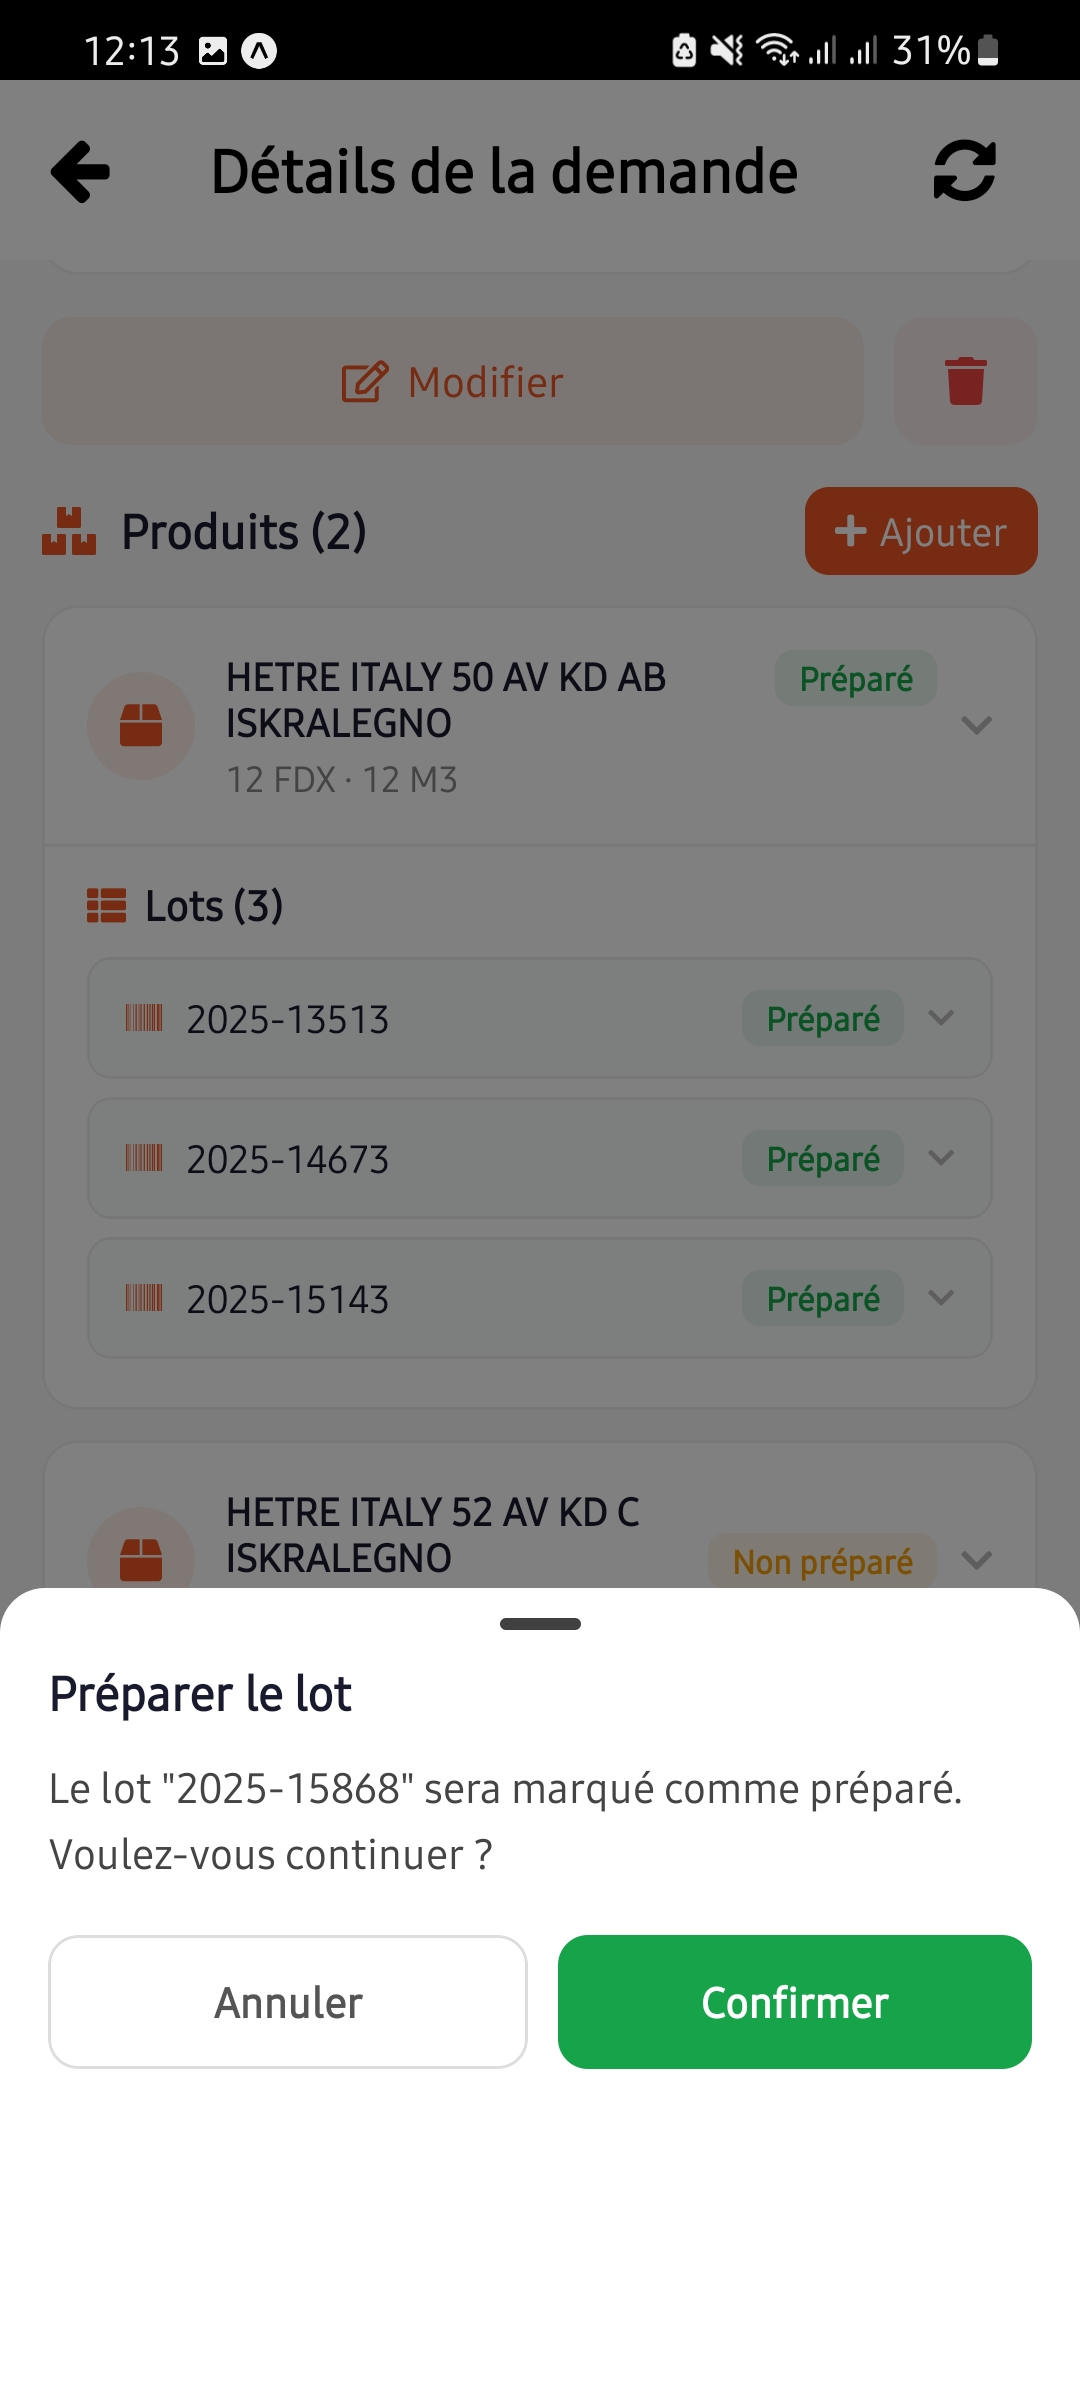
\includegraphics[width=0.75\textwidth]{assets/dt-preparer-lot.jpg}
    }{
    \textit{Préparation lot : fichier assets/dt-preparer-lot.jpg non trouvé.}
    }
    \caption{Préparer un lot}
    \label{fig:dt-preparer-lot}
    \end{minipage}
    \end{figure}

    \subsubsection{Création d'une demande de transfert}

    L'écran de création comporte un formulaire avec six champs : Dépôt source et Dépôt destination (sélectionnés via une feuille modale de liste de dépôts), DUM, Transporteur, Matricule et Observation (facultatif). La validation exige que les deux dépôts soient sélectionnés et que les champs DUM, Transporteur et Matricule soient renseignés.

    La Figure~\ref{fig:dt-create} présente l'écran de création avec le formulaire et les sélecteurs de dépôts.

    \begin{figure}[H]
    \centering
    \IfFileExists{assets/dt-create.jpg}{
    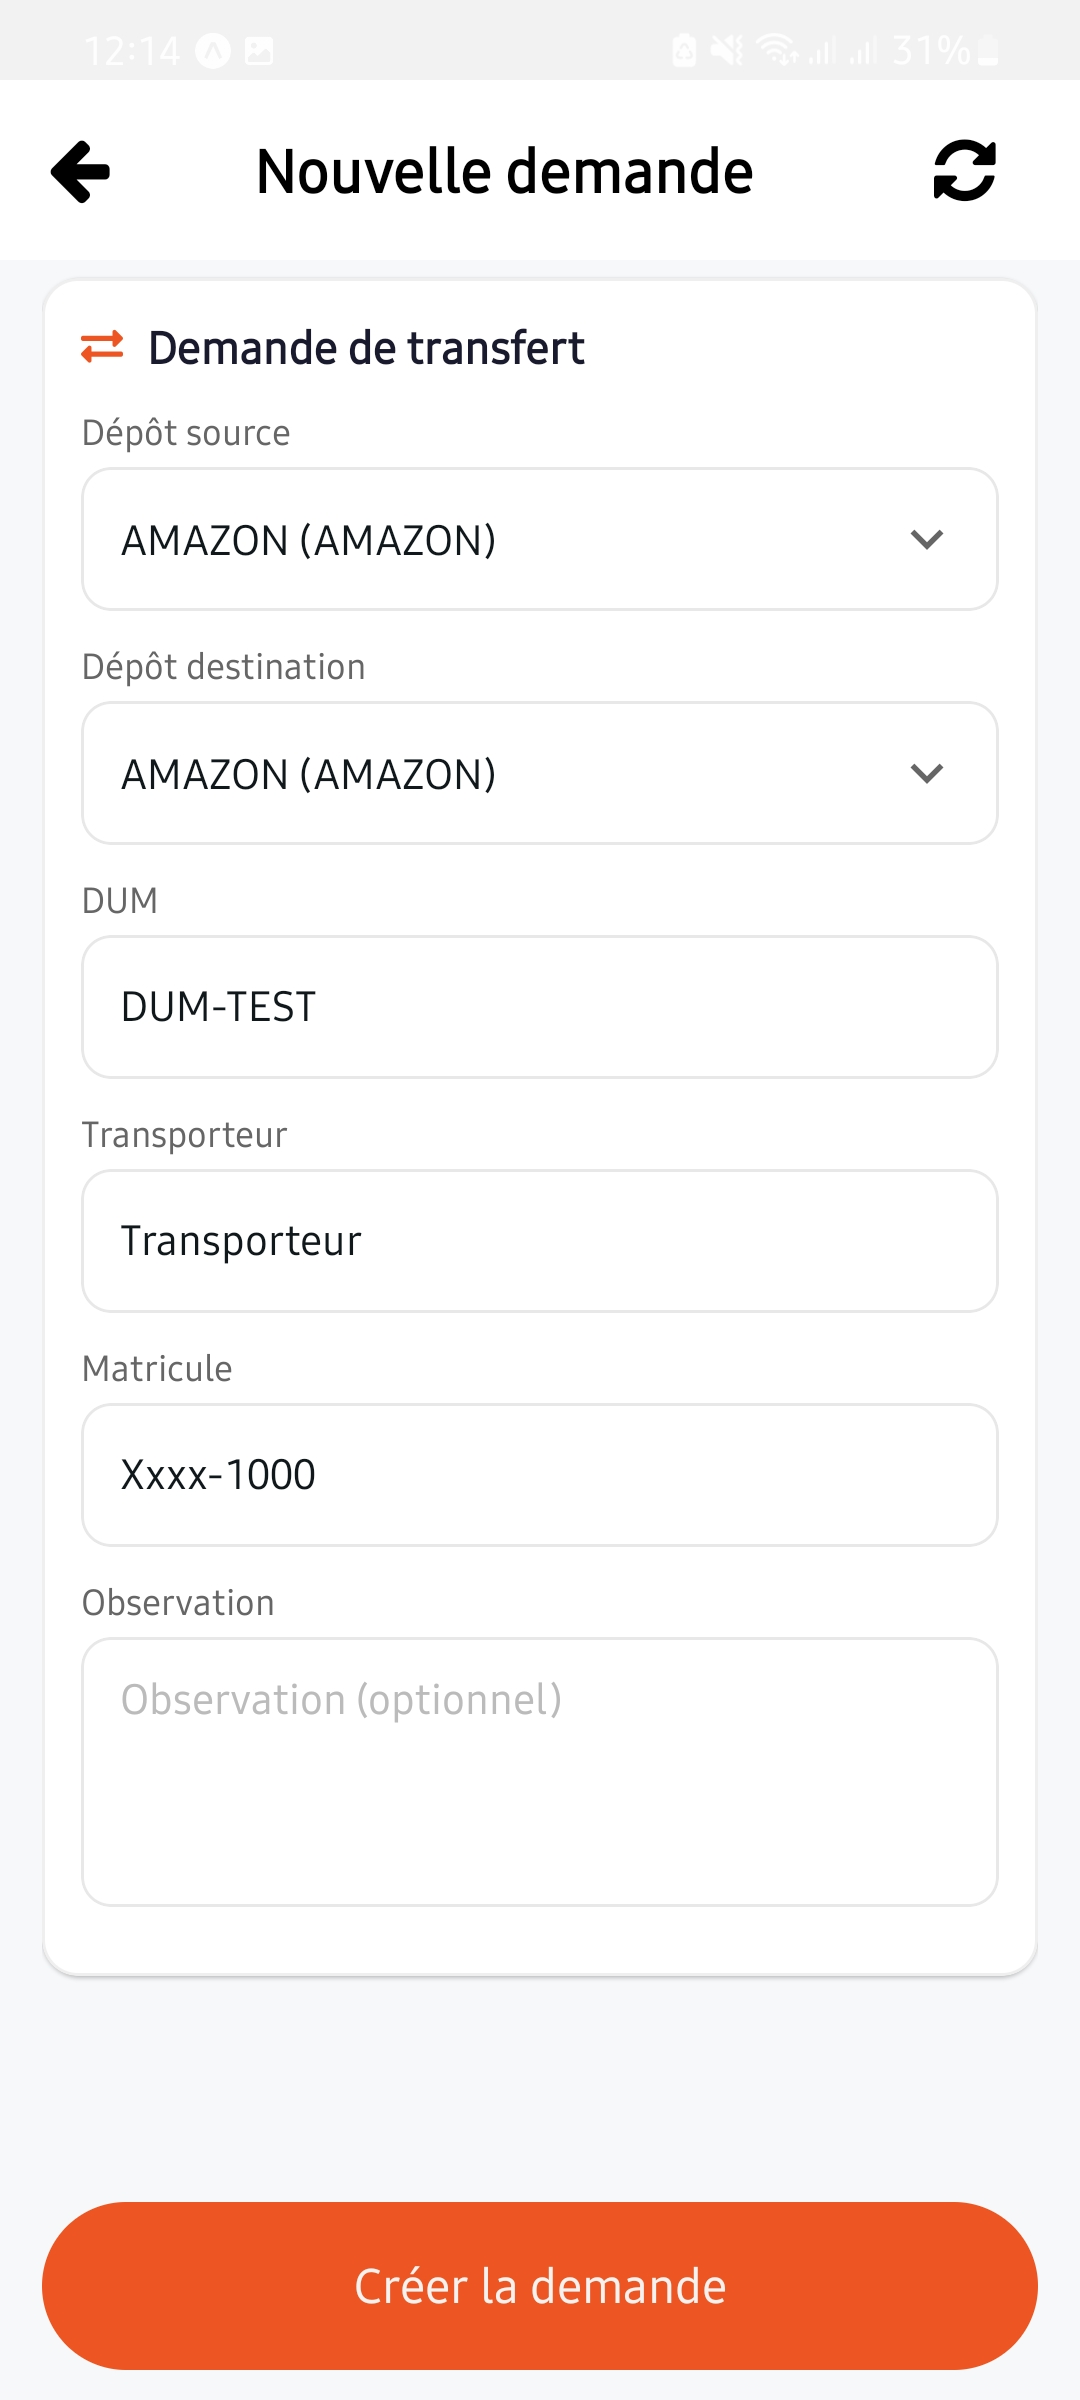
\includegraphics[width=0.25\textwidth]{assets/dt-create.jpg}
    }{
    \textit{Écran de création : fichier assets/dt-create.jpg non trouvé.}
    }
    \caption{Création d'une demande de transfert}
    \label{fig:dt-create}
    \end{figure}

    \section{Tests et validation}

    La stratégie de test adoptée pour ce projet repose sur une approche de tests manuels, couvrant à la fois le backend et le frontend. Cette approche, bien que plus légère qu'une suite de tests automatisés, s'est avérée adaptée au contexte du projet : une petite équipe Scrum avec des sprints de trois semaines et une application métier dont les flux sont bien définis.

    \subsection{Tests backend : API REST avec Postman}

    Chaque endpoint de l'API REST a été testé manuellement via Postman. L'outil a permis de vérifier le bon fonctionnement des opérations CRUD pour chaque module métier, de contrôler les codes de statut HTTP retournés (200, 201, 400, 404, 500), de valider la structure des réponses JSON et de s'assurer de la persistance correcte des données dans la base MySQL. Les scénarios de test incluent notamment : l'authentification avec jeton valide et invalide, la création d'entités avec champs obligatoires et facultatifs, la mise à jour partielle et complète, la suppression avec vérification de l'intégrité référentielle, et la pagination des listes.

    La Figure~\ref{fig:postman-test} illustre un test d'API réalisé avec Postman.

    \begin{figure}[H]
    \centering
    \IfFileExists{assets/postman-test.jpg}{
    \includegraphics[width=0.75\textwidth]{assets/postman-test.jpg}
    }{
    \textit{Test Postman : fichier assets/postman-test.jpg non trouvé.}
    }
    \caption{Test d'un endpoint API avec Postman}
    \label{fig:postman-test}
    \end{figure}

    \subsection{Tests frontend : Android Emulator et Expo Go}

    Le frontend a été testé de deux manières complémentaires. D'une part, l'émulateur Android (via Android Studio) a permis de simuler l'application sur différentes configurations d'écran et versions d'Android, garantissant une compatibilité large. D'autre part, Expo Go a été utilisé pour tester l'application en conditions réelles : rechargement instantané du code modifié, interaction tactile réelle et test sur périphérique physique.

    Les tests frontend ont couvert : le rendu de chaque écran avec données réelles, la navigation entre les écrans et le drawer, les interactions utilisateur (appuis, défilement, saisie, sélection), l'affichage des états de chargement et d'erreur, la validation des formulaires (champs requis, limites de fichiers) et la vérification du contrôle d'accès par permissions (affichage conditionnel des boutons et modules).

    La Figure~\ref{fig:expo-go-test} présente l'application en cours de test avec Expo Go sur un périphérique Android.

    \begin{figure}[H]
    \centering
    \IfFileExists{assets/expo-go-test.jpg}{
    \includegraphics[width=0.5\textwidth]{assets/expo-go-test.jpg}
    }{
    \textit{Test Expo Go : fichier assets/expo-go-test.jpg non trouvé.}
    }
    \caption{Interface développeur Expo Go — application en test}
    \label{fig:expo-go-test}
    \end{figure}

    \section{Conclusion}

    Ce chapitre a détaillé la mise en œuvre de la solution : outils (VS Code, Git, GitHub, Postman, phpMyAdmin, Android Studio), technologies (MySQL, PHP, TypeScript, React Native, Expo), architecture (backend Transaction Script, frontend en couches avec React Query et Zustand) et versionnement GitHub.

    La réalisation s'est articulée autour de quatre sprints : Sprint~2 (authentification et Voyages), Sprint~3 (Retours chauffeur et Rapports qualité), Sprint~4 (Rotation et Lieux de projets), Sprint~5 (Demande de transfert). Les tests manuels via Postman et l'émulateur Android/Expo Go ont validé l'ensemble des fonctionnalités, livrant une application mobile complète répondant aux besoins métiers de SDK WOOD.

    \newpage

\addcontentsline{toc}{section}{{\bfseries Conclusion générale}}

    \section*{Conclusion générale}

    Ce projet de fin d'année a permis de concevoir et de développer une application mobile complète répondant aux besoins métiers de SDK WOOD dans le domaine de la gestion logistique. L'application digitalise six modules fonctionnels — Voyages, Retours chauffeur, Rapports qualité, Rotation, Lieux de projets et Demande de transfert — couvrant l'ensemble du flux opérationnel des chauffeurs et agents sur le terrain.

    La réalisation de ce projet s'est appuyée sur une méthodologie agile Scrum, structurée en cinq sprints itératifs de trois semaines. Cette approche a permis une livraison incrémentale des fonctionnalités, une adaptation continue aux besoins métier et une validation régulière des incréments produits. Les rôles Scrum (Product Owner, équipe de développement, Scrum Master) et les rituels (Daily Scrum, Sprint Review, Sprint Retrospective) ont assuré une coordination efficace et une qualité continue.

    Sur le plan technique, le projet a mobilisé un éventail de technologies modernes : React Native et Expo pour le frontend mobile multiplateforme, TypeScript pour le typage statique et la maintenabilité, PHP et MySQL pour le backend s'intégrant à l'infrastructure existante, et une architecture en Transaction Script privilégiant la simplicité et la maîtrise du code. La gestion d'état a été confiée à React Query pour le cache serveur et Zustand pour l'état client, tandis que GitHub a assuré le versionnement et la traçabilité du code.

    La stratégie de tests manuels, combinant Postman pour les API REST et l'émulateur Android couplé à Expo Go pour le frontend, a permis de valider l'ensemble des fonctionnalités avec des données réelles avant la livraison.

    \subsection*{Perspectives}

    Bien que l'application réponde aux besoins actuels de SDK WOOD, plusieurs perspectives d'évolution peuvent être envisagées pour enrichir et étendre la solution :

    \begin{itemize}[leftmargin=1.2em]
    \item \textbf{Géolocalisation en temps réel} : intégration d'un suivi GPS en direct des véhicules de livraison, permettant une visualisation cartographique des tournées et une optimisation des itinéraires.

    \item \textbf{Notifications push} : mise en place de notifications instantanées pour informer les chauffeurs des nouvelles missions, des changements d'affectation ou des validations de retours.

    \item \textbf{Mode hors ligne} : implémentation d'un cache local persistant permettant aux chauffeurs de poursuivre leur travail en zones de faible connectivité, avec synchronisation automatique au retour du réseau.

    \item \textbf{Tableau de bord analytique} : développement d'une interface web d'administration avec statistiques et indicateurs de performance (KPI) — taux de livraison à temps, volume de retours, temps moyen par tournée — pour le pilotage opérationnel de la direction.

    \item \textbf{Signature électronique} : ajout d'une fonctionnalité de signature digitale des bons de livraison directement sur l'application, renforçant la traçabilité et la valeur probante des livraisons.

    \item \textbf{Tests automatisés} : mise en place d'une suite de tests unitaires et d'intégration (Jest, React Native Testing Library) ainsi que de tests end-to-end (Detox) pour garantir la non-régression lors des futures évolutions.

    \item \textbf{Déploiement iOS} : extension du déploiement vers l'App Store via EAS Build et certification Apple, afin de couvrir l'écosystème iOS en complément d'Android.

    \item \textbf{Intégration avec un système ERP} : connexion de l'application à un système de gestion d'entreprise (ERP) pour synchroniser automatiquement les stocks, les commandes et les factures, évitant ainsi la double saisie.
    \end{itemize}

    Ces perspectives ouvrent des voies d'amélioration concrètes qui permettront à SDK WOOD de poursuivre la digitalisation de son activité logistique et de renforcer sa compétitivité sur le marché.

    \newpage
    \addcontentsline{toc}{section}{\bfseries Bibliographie}
    \section*{Bibliographie}

    \begin{thebibliography}{99}

    \bibitem{scrum}
    K. Schwaber et J. Sutherland, \textit{The Scrum Guide -- The Definitive Guide to Scrum: The Rules of the Game}, Scrum.org, 2020. \url{https://www.scrumguides.org/scrum-guide.html}

    \bibitem{reactnative}
    Meta Open Source, \textit{React Native -- Official Documentation}, 2024. \url{https://reactnative.dev/docs/getting-started}

    \bibitem{expo}
    Expo, \textit{Expo Documentation -- SDK, EAS Build et Expo Go}, 2024. \url{https://docs.expo.dev/}

    \bibitem{typescript}
    Microsoft, \textit{TypeScript Handbook}, 2024. \url{https://www.typescriptlang.org/docs/handbook/intro.html}

    \bibitem{php}
    The PHP Group, \textit{PHP Manual -- Server-side scripting language}, 2024. \url{https://www.php.net/manual/en/}

    \bibitem{mysql}
    Oracle Corporation, \textit{MySQL Reference Manual}, 2024. \url{https://dev.mysql.com/doc/refman/8.0/en/}

    \bibitem{fowler}
    M. Fowler, \textit{Patterns of Enterprise Application Architecture}, Addison-Wesley Professional, 2002, chap. « Transaction Script ».

    \bibitem{uml}
    OMG (Object Management Group), \textit{Unified Modeling Language (UML) Specification}, version 2.5.1, 2017. \url{https://www.omg.org/spec/UML/2.5.1/}

    \bibitem{apache}
    Apache Software Foundation, \textit{Apache HTTP Server Documentation}, 2024. \url{https://httpd.apache.org/docs/2.4/}

    \bibitem{reactquery}
    TanStack, \textit{React Query -- Data-fetching library for React}, 2024. \url{https://tanstack.com/query/latest}

    \bibitem{zustand}
    Poimandres, \textit{Zustand -- Bear necessities for state management in React}, 2024. \url{https://github.com/pmndrs/zustand}

    \bibitem{androidstudio}
    Google, \textit{Android Studio -- Official IDE for Android development}, 2024. \url{https://developer.android.com/studio}

    \bibitem{postman}
    Postman Inc., \textit{Postman Documentation -- API development and testing platform}, 2024. \url{https://learning.postman.com/}

    \bibitem{git}
    Software Freedom Conservancy, \textit{Git -- Distributed Version Control System}, 2024. \url{https://git-scm.com/doc}

    \bibitem{github}
    GitHub Inc., \textit{GitHub Documentation -- Code hosting and collaboration}, 2024. \url{https://docs.github.com/}

    \bibitem{phpmyadmin}
    phpMyAdmin Team, \textit{phpMyAdmin Documentation -- MySQL web administration}, 2024. \url{https://docs.phpmyadmin.net/}

    \bibitem{rest}
    R. T. Fielding, \textit{Architectural Styles and the Design of Network-based Software Architectures}, Ph.D. dissertation, University of California, Irvine, 2000, chap. 5 « Representational State Transfer (REST) ».

    \bibitem{onfleet}
    Onfleet Inc., \textit{Onfleet -- Last Mile Delivery Management Software}, 2024. \url{https://onfleet.com/}

    \bibitem{samsara}
    Samsara Inc., \textit{Samsara -- Connected Operations Cloud}, 2024. \url{https://www.samsara.com/}

    \bibitem{vscode}
    Microsoft, \textit{Visual Studio Code Documentation}, 2024. \url{https://code.visualstudio.com/docs}

    \bibitem{expo-router}
    Expo, \textit{Expo Router -- File-based routing for React Native}, 2024. \url{https://docs.expo.dev/router/installation/}

    \end{thebibliography}

    \end{document}
